% \iffalse meta-comment
%<*internal>
\iffalse
%</internal>
%<*readme>
----------------------------------------------------------------
phd --- a package to shorten preambles
E-mail: yannislaz@gmail.com
Released under the LaTeX Project Public License v1.3c or later
See http://www.latex-project.org/lppl.txt
----------------------------------------------------------------
This file provides a phd for defining a class.
%</readme>
%<*readmemd>
###The `phd` LaTeX2e package

This latex package and the class with the same name provide
convenient methods to create new styles for books, reports
and articles. It also preloads the most commonly used packages 
and resolves conflicts.

This work consists of the file  `phd.dtx`,
and the derived files   `phd.ins`,  `phd.pdf`, and `phd.sty`.

###Installation

run
          
           pdflatex phd.dtx
           makeindex -s gind.ist phd.idx

If you have any difficulties with the package come and join us at
http://tex.stackexchange.com and post a new question or
add a comment at http://tex.stackexchange.com/a/45023/963.
or send me a message at  yannislaz at gmail.com

%</readmemd>
%
%<*TODO>
add tcolorbox support c
%</TODO>
%<*internal>
\fi
\def\nameofplainTeX{plain}
\ifx\fmtname\nameofplainTeX\else
  \expandafter\begingroup
\fi
%</internal>
%<*install>
\input docstrip.tex

\askforoverwritefalse
\preamble
----------------------------------------------------------------
phd --- short description.
E-mail: yannislaz@gmail.com
Released under the LaTeX Project Public License v1.3c or later
See http://www.latex-project.org/lppl.txt
----------------------------------------------------------------

\endpreamble

\usedir{tex/latex/phd}
\generate{\file{\jobname.sty}{\from{\jobname.dtx}{package}}}
\generate{
  \file{MWE-02.tex}{\from{\jobname.dtx}{MWE-02}}
  \file{MWE-03.tex}{\from{\jobname.dtx}{MWE-03}}
}
\generate{
  \file{test-tufte.tex}{\from{\jobname.dtx}{test-tufte}}
  \file{test-memoir.tex}{\from{\jobname.dtx}{test-memoir}}
  \file{test-scrartcl.tex}{\from{\jobname.dtx}{test-scrartcl}}
  \file{test-algorithms.tex}{\from{\jobname.dtx}{test-algorithms}}
  \file{test-hyphenation.tex}{\from{\jobname.dtx}{test-hyphenation}}
  \file{settings.tex}{\from{\jobname.dtx}{settings}}
  \file{test-spacing.tex}{\from{\jobname.dtx}{test-spacing}}
 }
%</install>
%<install>\endbatchfile
%<*internal>
\usedir{tex/latex/phd}
\generate{
  \file{\jobname.ins}{\from{\jobname.dtx}{install}}
}
\nopreamble\nopostamble
\usedir{source/phd}
\generate{
  \file{README.txt}{\from{\jobname.dtx}{readme}}
}
\generate{
  \file{README.md}{\from{\jobname.dtx}{readmemd}}
}
\generate{
  \file{TODO.tex}{\from{\jobname.dtx}{TODO}}
}
\generate{
  \file{MWE-01.tex}{\from{\jobname.dtx}{MWE-01}}
}
\ifx\fmtname\nameofplainTeX
  \expandafter\endbatchfile
\else
  \expandafter\endgroup
\fi
%</internal>
%<*driver>
\listfiles
\documentclass[reqno,oneside,11pt,letter,a4paper]{ltxdoc}
\usepackage[pass]{geometry}

\newgeometry{left=3.5cm,right=3.5cm,top=2.0cm,bottom=1.5cm,
    marginparsep=5mm,marginparwidth=10mm,
    %headheight=0mm,headsep=0cm,
    footskip=1.5cm,includeheadfoot}
\setcounter{secnumdepth}{6}
\usepackage[T1]{fontenc}
%\usepackage{libertine}
%\renewcommand{\ttfamily}{\fontencoding{OT1}\fontfamily{cmtt}\selectfont}
\usepackage{lmodern,algorithm2e} %lmodern,
\usepackage[toc,lof,lot]{multitoc}
\usepackage{fancyhdr,picture}
%\usepackage{dateiliste}
\usepackage{\jobname}
%\usepackage[listings,theorems]{tcolorbox}
\tcbset{before={\par\medskip\pagebreak[0]\noindent},after={\par\medskip}}%
%\usepackage{multicol}
\def\AmSmath{AmSmath}
%
% The hypdoc loads the {hyperref}[2002/05/09] package with
% certain options.
%

\usepackage{hyperref}[2012/02/06]
% hyperdoc has a problem with tcolorboc documentation
% macros.
%\usepackage{hypdoc}
\hypersetup{pdftex,
  bookmarks,
  raiselinks,
  pageanchor,
  hyperindex,
  colorlinks,
  allcolors=theblue, 
  %anchorcolor= blue,
  %filecolor=blue,
  urlcolor= teal,
  linkcolor= teal,
  pdftitle={My Title},
  pdfauthor={Yiannis Lazarides},
  pdfsubject={The phd LaTeX package},
  pdfkeywords={LaTeX package management, document design}
 }


% add pdfinfo  
% 
% 
%\newcommand*{\file}[1]{\texttt{#1}}
\newcommand*{\pkg}[1]{\texttt{#1}}
%\usepackage[numbered]{hypdoc}
\definecolor{lstbgcolor}{rgb}{0.9,0.9,0.9}
\newcommand*{\Lpack}[1]{\textsf {#1}}  
\let\package\Lpack
\makeatletter
% mock chapters where necessary
\@ifundefined{c@chapter}{%  
      \newcounter{chapter}
      \def\thechapter{}
}{}

\cxset{plain sections/.style={
 chapter name = CHAPTER,
 chapter toc = true,
 chapter color= thegray,
 chapter opening = right, 
 chapter numbering = arabic,
 chapter font-family= sffamily,
 chapter font-weight= bold,
 chapter font-size= LARGE,
 chapter before={\thinrule\vspace*{20pt}\par\hfill\hfill},
 chapter after={\vskip0pt\par},
 chapter spaceout = soul,
 number font-size= Large,
 number font-family= rmfamily,
 number font-weight= bfseries,
 number color=thegray,
 number before=\vspace*{5pt}\hfill\hfill,
 number dot=.,
 number after={\hspace*{7pt}\par},
 title beforeskip={\vspace*{10pt}},
 title afterskip={\vspace*{50pt}\par},
 title before={\hfill\hfill\raggedleft},
 title after={\par\thinrule},
 title font-family=\sffamily,
 title font-color= teal,
 title font-weight=\bfseries,
 title font-family=\sffamily,
 title font-size= Large,
 title font-shape=\upshape,
 title spaceout= none,
  title beforeskip={\vspace*{10pt}},
 title afterskip={\vspace*{50pt}\par},
 title before={\hfill\hfill\raggedleft},
%
% numbers
% number font-family=\sffamily,
% number font-weight=\bfseries,
 number color=thelightgray,
 number before=\par\vspace*{5pt}\hfill\hfill,
 number dot=,
 number after={\hspace*{7pt}\par},
 number position=rightname,
 section color= thered,     
 section beforeskip=15pt,
 section afterskip=15pt,
 section indent=0pt,
 section font-family= sffamily,
 section font-size= LARGE,
       section font-weight= bfseries,
       section font-shape=,
       section align= centering,
       section numbering prefix =,%use \thechapter. for books or add as option
       section numbering= arabic,
       section spaceout=none,
       section number after=ooo,
       subsection color= thered,
       subsection beforeskip=10pt,
       subsection afterskip=10pt,
       subsection indent=0pt,
       subsection font-family= rmfamily,
       subsection font-size= large,
       subsection font-weight= bold,
       subsection font-shape=,
       subsection align= centering,
       subsection numbering prefix=\thesection.,%\S\hairsp,%add . 
       subsection numbering custom = \two@digits{\@arabic\c@subsection},%
       subsubsection color= thered,
       subsubsection beforeskip=5pt plus3pt minus 2pt,
       subsubsection afterskip=5pt,
       subsubsection indent=0pt,
       subsubsection font-family= rmfamily,
       subsubsection font-size= normalfont,
       subsubsection font-weight= bold,
       subsubsection font-shape= itshape,
       subsubsection align= centering,
       subsubsection numbering prefix = \thesubsection.,
       subsubsection numbering custom = \two@digits{\@arabic\c@subsubsection},
       subsubsection number after =, 
%
       paragraph color= thegrey,
       paragraph beforeskip=0pt,
       paragraph afterskip=-0.5em,
       paragraph indent=0pt,
       paragraph font-family= rmfamily,
       paragraph font-size= large,
       paragraph font-weight= bfseries,
       paragraph font-shape=,
       paragraph align= centering,
       paragraph number after =,
       paragraph numbering=numeric,
       subparagraph color= thered,
       subparagraph beforeskip=0pt,
       subparagraph afterskip=-.5em,
       subparagraph indent=0pt,
       subparagraph font-family= sffamily,
       subparagraph font-size= large,
       subparagraph font-weight= normalfont,
       subparagraph font-shape= slshape,
       subparagraph align= RaggedRight,
       subparagraph number after =, % can affect all needs checking
       %subsubsection numbering prefix=\S\hairsp\thesection,%add . here if need be
       subparagraph numbering=none,
}
}

\cxset{plain sections}
\cxset{style13/.style={
 name=CHAPTER,
 numbering=arabic,
 number font-size= HUGE,
 number font-family= sffamily,
 number font-weight= bfseries,
 number color= gray!50,
 number before=\par\vspace*{5pt}\hfill\hfill,
 number dot=,
 number after={\hspace*{7pt}\par},
 number position=rightname,
 chapter font-family= sffamily,
 chapter font-weight= normalfont,
 chapter font-size= LARGE,
 chapter before={\thinrule\vspace*{20pt}\par\hfill\hfill},
 chapter color= black!50,
 title beforeskip={\vspace*{10pt}},
 title afterskip={\vspace*{50pt}\par},
 title before={\hfill\hfill\raggedleft},
 title after=\par\thinrule,
 title font-family= sffamily,
 title font-color= teal,
 title font-weight= bfseries,
 title font-size= huge,
 section indent=-1em,
 section align= left,
 section numbering=arabic,
 section indent=0pt,
 section beforeskip=0pt,
 section afterskip= 10pt,
 section color=teal,
 subsection align= ,
 subsection font-family= sffamily,
 subsection font-weight= bfseries,
 subsection color = teal,
 subsection font-size= large,
 subsection font-shape= itshape,
 subparagraph number after=,
 subsubsection align=,
}
}

\def\oarg#1{%
  \colOpt{{\ttfamily[}\meta{#1}{\ttfamily]}}}

\cxset{style13}
\makeatletter
\renewparagraph
\renewsection
\renewsubparagraph
\renewsubsubsection

 \makeatother
%%http://tex.stackexchange.com/questions/75055/print-filelist-to-pdf/75064#75064
%\printFileList
%
% COMMENT THE NEXT LINE TO INCLUDE THE CODE
% \AtBeginDocument{\OnlyDescription}
\EnableCrossrefs
\CodelineIndex
\RecordChanges
\begin{document}
    \DocInput{\jobname.dtx}
\end{document}
%</driver>
% \fi
%
%  \CheckSum{3167}
%  \CharacterTable
%  {Upper-case    \A\B\C\D\E\F\G\H\I\J\K\L\M\N\O\P\Q\R\S\T\U\V\W\X\Y\Z
%   Lower-case    \a\b\c\d\e\f\g\h\i\j\k\l\m\n\o\p\q\r\s\t\u\v\w\x\y\z
%   Digits        \0\1\2\3\4\5\6\7\8\9
%   Exclamation   \!     Double quote  \"     Hash (number) \#
%   Dollar        \$     Percent       \%     Ampersand     \&
%   Acute accent  \'     Left paren    \(     Right paren   \)
%   Asterisk      \*     Plus          \+     Comma         \,
%   Minus         \-     Point         \.     Solidus       \/
%   Colon         \:     Semicolon     \;     Less than     \<
%   Equals        \=     Greater than  \>     Question mark \?
%   Commercial at \@     Left bracket  \[     Backslash     \\
%   Right bracket \]     Circumflex    \^     Underscore    \_
%   Grave accent  \`     Left brace    \{     Vertical bar  \|
%   Right brace   \}     Tilde         \~}
%
%
% \changes{1.0}{2013/01/26}{Converted to DTX file}
% \changes{1.01}{2013/01/27}{Added multicol}
% \DoNotIndex{\newcommand,\newenvironment}
% \GetFileInfo{phd.dtx}
% \providecommand*{\url}{\texttt}
%  \def\fileversion{v1.0}          
%  \def\filedate{2012/03/06}
% \title{The \textsf{phd} package.
% \thanks{This
%        file (\texttt{phd.dtx}) has version number \fileversion, last revised
%        \filedate.}
% }
% \author{Dr. Yiannis Lazarides \\ \url{yannislaz@gmail.com}}
% \date{\filedate}
%
%
% 
% ^^A\maketitle
% \pagestyle{empty}
% \frontmatter
% \coverpage{hine02}{Yiannis Lazarides}{Published by Camel Press}
% \secondpage
% \pagestyle{empty}
%
%
% ^^A Table of contents in two columns --- borrowed from the standard 
% ^^A package of ``doc.dtx''
% 
% \newif\ifmulticols
% \IfFileExists{multicol.sty}{\multicolstrue}{}
%
% ^^A\ifmulticols
% ^^A\addtocontents{toc}{\protect\begin{multicols}{2}}
% ^^A\fi
%
% {\parskip 0pt                ^^A We have to reset \parskip
% \gdef\dotsep{10000}          ^^A (bug in \LaTeX)
% \tableofcontents
% \listoftables
% \listoffigures
% }
% 
% \mainmatter
%
% \makeatletter\@specialfalse\makeatother
\parindent1em
\cxset{section align=left}
\cxset{toc image= ted_turner_2001,
          subsection color=black,
          section color=black,
          subsubsection numbering=arabic,
          subsubsection color=black,
          subsubsection font-shape=upshape}
\chapter{TOC Styling}
\label{ch:toc}

\precis{In this chapter we outline a number of settings that have been defined to handle Table of Contents (ToC) formatting. We also review the technical issues facing the construction of Table of Contents and their variants. The relationship of the hyperref package to the ToC and the many issues arising out of it are also discussed.}
\addtocimage{-12pt}{-20pt}{../images/tocblock-rooster.jpg}



\section{Introduction}

The setting of parameters for the |ToC|, is a bit more complex than those for sectioning commands. It also requires that one has a good understanding of \latexe terminology. However, t set they are easy to change afterwards.
The \pkgname{phd} also provides a number of predefined ones.

An entry line to the |ToC| can be though of consisting of four components. The entry type (chapter, section etc.), number, title and page number. This presents a similar problem to that of styling sectioning commands to parametrize it in such a way as to provide a fully flexible system. The code provided by \latexe is complicated and difficult to parameterize it. Ideally we would like a fully flexible system that can be moulded into  


\oldcontentsline{section}{heading title}{\thepage}

\contentsline{section}{heading title}{\thepage}{chapter.1}

\contentsline {section}{\numberline {}Introduction}{5}{section.2.1}


\section{Key values for Chapters}


\begin{key}{/phd/toc levels = \meta{number}}
 Equivalent parameterized key to |\toclevel|. It sets  the \texttt{tocdepth} counter. If empty no toc is defined. LaTeX uses this to determine how many levels of toc are included.
\end{key}

\begin{key}{/phd/toc number width = marg{dimension}\cs{@pnumwidth}}
The key sets the width of the numbers in the ToC. 
\end{key}

\subsection{Spacing Keys}
\begin{key}{/phd/toc chapter number color=\meta{color name}}
This key will set the color of the chapter number.
\end{key}

\begin{key}{/phd/toc chapter beforeskip=\meta{length}}
The amount of glue to insert before the toc chapter line.
\end{key}

\begin{key}{/phd/toc chapter afterskip=\meta{length}}
The amount of glue to insert before the toc chapter line.
\end{key}

\begin{key}{/phd/toc chapter indent=\meta{length}}
The amount of glue to indent the line.
\end{key}
\subsection{Hooks}


\makeatletter
\def\options#1{
\@for\next:=#1\do{%
\textbar\next%
}%
\textbar%
}%
\options{test1,test2,test3}
\makeatother
\begin{key}{/phd/toc dots = \textbar none\textbar false\textbar true}
\end{key}

\begin{marglist}
 \item[none] this sets the value of \cs{@dotsep} to 1000 thus eliminating the dots.
\item [false] alias for the above key.
\item [true] dot leaders are used, uses a default value for \cs{@dotsep} of 4.5,
\end{marglist}
\keyval{toc dotsep}{\marg{number}}{renewcommand  @dotsep}
\keyval{toc chapter name}{}{chaptername}
\keyval{toc chapter name color}{}{tocchapternamecolor@cx}
\keyval{toc title color}{}{toctitlecolor@cx}
\keyval{toc title font-weight}{}{toctitlefontweight@cx}
\keyval{toc title before}{}{toctitlebefore@cx}
\keyval{toc title after}{}{toctitleafter@cx}
\keyval{toc after pagenumber}{}{tocafterpagenumber@cx}
\keyval{toc right margin}{}{@tocrmarg}
\keyval{toc number after}{}{tocnumberafter@cx}
\keyval{toc image}{\marg{filename}}{If the TOC has images associated with chapters these are used in the typesetting. Used with custom templates.}
\keyval{toc custom}{\marg{cmd}}{Triggers the loading of alternative templates than those structured by LaTeX.}
\keyval{hypersetup linkcolor}{\marg{color}}{Changes the color of a hyperlink. This is experimental and better used at document level.}
\keyval{toc chapter precis}{\marg{true|false}}{This is experimental. If a chapter precis is specified in a chapter, then the precis is typeset in the ToC also\footnote{Such a command is provided by the \pkg{tocloft} package and in the memoir class}.}

\section{Styling the sections in the ToC}

\begin{key}{/phd/toc section beforeskip = \meta{length}}
\end{key}
\begin{key}{/phd/toc section afterskip = \meta{length}}
\end{key}
\begin{key}{/phd/toc section indent = \meta{length}}
\end{key}

\begin{verbatim}
\cxset{toc section beforeskip/.store in=\tocsectionbeforeskip@cx,
       toc section indent/.store in=\tocsectionindent@cx,
%      fonts for title &num
       toc section font-size/.store in=\tocsectionfontsize@cx, 
       toc section font-family/.store in=\tocsectionfontfamily@cx, 
       toc section font-shape/.store in=\tocsectionfontshape@cx, 
       toc section font-weight/.store in=\tocsectionfontweight@cx, 
       toc section color/.store in=\tocsectioncolor@cx,
       toc section numwidth/.store in=\tocsectionnumwidth@cx,
%	  fonts etc for page number
       toc section page font-size/.store in=\tocsectionpagefontsize@cx,
       toc section page font-family/.store in=\tocsectionpagefontfamily@cx,
       toc section page font-shape/.store in=\tocsectionpagefontshape@cx,
       toc section page font-weight/.store in=\tocsectionpagefonteight@cx,
       toc section page color/.store in=\tocsectionpagecolor@cx,
%      leaders
	 toc section dotsep/.store in = \tocsecdotsep@cx,
%      before and after page number
       toc section page before/.store in=\tocsectionpagebefore@cx,
       toc section page after/.store in=\tocsectionpageafter@cx,
}
\end{verbatim}

Firstly we define the width of the box that the page number is set. Use ems so that it does not need to be redefined for every change in font size.
ToC entries are treated as rectangular areas where the text
and probably a filler will be written. Let's draw such an
area (of course, the lines themselves are not printed):



\section{Other Packages and Classes}
The package \pkg{tocloft} provides  provides handles for an author to change the design to meet the needs of the particular document, by providing a number of settings commands.


%\addtocontents{toc}{\colorbox{cyan}{\thesection this is some long command \thepage}}

\section{Technical Details}

In the standard classes the design of the Table of Contents (ToC) the List of Figures (LoF) and list of tables (LoT) is fixed and buried within the class definitions.

\begin{macro}{\addcontentsline}
\begin{macro}{\addcontents}
To understand the way \LaTeX\ formats the ToC, one has to understand that the ToC entries are generated and typeset in different operations. Firstly when the document is processed, every time a sectioning command such as \cs{chapter} or \cs{section} is activated it calls on either the macro \cs{addcontentsline} or \cs{addcontents}, which in turn will initiate the process of writing the entry onto a file.
\end{macro}
\end{macro}


\subsection{Reading from the ToC file}

\begin{macro}{\tableofcontents}
The second operation happens when \latexe sees a \cs{tableofcontents} command. This initiates the read operation, where the information that has been stored in the ToC file is read and typeset.
\end{macro}


\subsubsection{Initiating reading of the ToC, the \texttt{\textbackslash tableofcontents} command}

We should start dissecting the algorithm by first viewing the \cs{tableofcontents}. This command is provided in
the standard classes (see \pageref{tableofcontents}) and it does not take any parameters.

\begin{teX}
\setcounter{tocdepth}{2}
\newcommand\tableofcontents{%
    \if@twocolumn
      \@restonecoltrue\onecolumn
    \else
      \@restonecolfalse
    \fi
    \chapter*{\contentsname
        \@mkboth{%
           \MakeUppercase\contentsname}{\MakeUppercase\contentsname}}%
          \@starttoc{toc} (*@\label{starttoc}@*)
    \if@restonecol\twocolumn\fi
    }
\end{teX}


The important thing to notice here is that the words contents are typeset by calling the star version and hence the contents name is not added to the toc. If we needed to add it we need to explicitly add to the toc as well as format it, if necessary. The other notable item is the \cs{@starttoc}\marg{toc} macro. This command opens the |toc| file to read or write.

\subsubsection{The Contents heading}
 
 The \pkgname{phd}  package redefines the \cmd{\tableofcontents}  to call a specific macro to typeset
 the contents name and provides hooks to provide flexible styling. 
              
\begin{texexample}{Contents heading and hooks}{}
\sampletoctitle
\cxset{toc name=Inhalt,
          toc name color=black,
          toc name align=left,
          toc name indent=,
          toc name before=\topline\par,
          toc name after=\par\bottomline\par}
\sampletoctitle
\cxset{toc name=Contents,
          toc name case=none,
          toc name color=black,
          toc name align=none,
          toc name indent=\hspace*{4.2cm},
          toc name before=\hspace*{4.2cm}\rule{\textwidth-4.2cm}{1pt}\vskip1.5pt,
          toc name after=\par\vskip30pt\bottomline\par,
          toc name font-size=Huge,
          toc name font-family=rmfamily}
          
\sampletoctitle
\end{texexample}

The last example is from an Oxford University Press publication \textit{Portraiture}. It would never pass my mind to design such a Contents page style, but it does look and is a good test for our code  (Figure~\ref{tocsample}). Our spacing looks odd, as the geometry of the page is different as well as the selection of font. This design is found in the full Oxford History of Art series.

\begin{figure}[htbp]
\centering
\includegraphics[width=0.8\textwidth]{oxford-toc}
\caption{Spread with ToC starting page from \textit{Portraiture}.}
\label{tocsample}
\end{figure}

While we at it, let us go over one more example. This time the template is shown in Figure~\ref{fig:reinvent}. This is a ruled example. The top rule will be at the beginning of the ToC and the bottom will be at the beginning of the Part. We will come back for the latter later.

\begin{figure}[htbp]
\centering
\includegraphics[width=0.5\textwidth]{reinvent}
\caption{Spread with ToC starting page from \textit{Reinvent Yourself}.}
\label{fig:reinvent}
\end{figure}

\begin{texexample}{Contents heading and hooks}{}
\def\doublerule{\hrule width\textwidth height1pt depth0pt\vskip1pt
     \hrule width\textwidth height3.5pt depth0pt\vskip24pt\relax}
\cxset{toc name=Contents,
          toc name case=none,
          toc name color=black,
          toc name align=center,
          toc name indent=, 
          toc name before=\doublerule,
          toc name font-size=Huge,
          toc name font-family=rmfamily}
 \sampletoctitle
\end{texexample}

What we have just done we defined a double rule macro and just inserted it as the argument before the name hook. The ``contents'' was typeset as is and centered align. 



\subsubsection{The \textbackslash @starttoc macro}

Remember when the \cmd{\tableofcontents} was intitiated it called the \cmd{\@starttoc} command in line \ref{starttoc}. This is defined in the LaTeX kernel and not in the class files. The \cmd{@starttoc}\meta{ext} command is used with the commands:
\cs{tableofcontents}, \cs{listoffigures}, etc. \footnote{See a more detailed explanation on ltsect.dtx, page 288.}

For example: \cs{@starttoc}{lof} is used in listoffigures. This command
reads the |.ext| and typesets it if avialable and sets up to write the new file. The reading operation always takes place (Line \ref{readtoc}). The |\@nobreakfalse| is globally set to allow breaks. 

\begin{teX}
\def\@starttoc#1{%
\begingroup
  \makeatletter
  \@input{\jobname.#1}% (*@\label{readtoc}@*)
  \if@filesw
    \expandafter\newwrite\csname tf@#1\endcsname
    \immediate\openout \csname tf@#1\endcsname \jobname.#1\relax
   \fi
   \@nobreakfalse
\endgroup}
\end{teX}

We can modify the command slightly in a group and load |phd.tst| a file I have created to see how it is working. For the time being let us ignore how we wrote to the file.

\begin{texexample}{Test ToC}{}
\makeatletter
\cxset{toc section color=black} 
\begingroup
\def\@starttoc#1{
    \@input{\jobname.#1}
    \@nobreakfalse}
\@starttoc{tst}  
\endgroup
\makeatother
\end{texexample}

The reason we have defined the command in a group---as well as called it---was to avoid redefining it and breaking this document and also not to waste another file as they are limited in TeX. This command it breaks with good programming practice, where functions should be defined to do one thing at a time it would have been preferable to have had |\@readtoc| and  |\@writetoc| commands. More about this later.

The file we have just read is as follows:

\begin{verbatim}
\select@language {english}
\contentsline {chapter}{\chapternumberline {1}{Introduction}{}}{1}{section*.2}
\addtocimage@cx {-12pt}{-20pt}{../images/tocblock-fish.jpg}
\contentsline {section}{\numberline {1}The key value concept}{2}{section.1.1}
\contentsline {subsection}{\numberline {1.1}Settings}{3}{subsection.1.1.1}
\contentsline {subsection}{\numberline {1.2}Cascading}{3}{subsection.1.1.2}
\end{verbatim}

The \cs{contentsline} definition triggers the calling of macros that start with \verb+l@+ and for the sectioning commands have typical formats such as \lstinline{\l@chapter, \l@section etc.} So in reality when we read the
file the comand:
\begin{teX}
\def\contentsline#1{\csname l@#1\endcsname}
\end{teX}
was expanded and absorbed the first parameter, for example |{section}| which then continued expanding to |\l@section| to absorb the balance parameters.

\begin{texexample}{Expansion of l@section}{}
\makeatletter
\l@section{\numberline {1}The key value concept}{2}{section.1.1}
\l@section{\numberline {1}The key value concept}{2}{}
\makeatother
\end{texexample}

\subsubsection{Hyperref}

The example did not work as advertized for the simple reason that hyperref interferes to pick the last parameter for its own purpose. As Peter Wilson says the \pkg{hyperref} package dislikes authors using
\cs{addcontentsline}. To get it to work properly with \pkg{hyperref}  you normally have to put \cs{phantomsection} (a macro defined within  the \pkg{hyperref} package) immediately  before \cs{addcontentsline}. This gave me considerable headaches when redefining these commands for special |ToC|s.
When we use hyperef we get an additional parameter |chapter.1| on line one and if we combine the example above, we will get errors of run away arguments.

\begin{texexample}{ToC example with hyperref}{ex:toc2}
\contentsline {chapter}{\numberline {1}First Chapter}{3}{chapter.1}
\contentsline {section}{\numberline {1.1}Introduction}{3}{section.1.1}
\contentsline {subsection}{\numberline {1.1.1}The difficulties}{3}{subsection.1.1.1}
\contentsline {chapter}{\numberline {2}Second Chapter}{5}{chapter.2}%
\end{texexample}

Predictably |hyperref| redefines the |\contentsline| command. We see from the documentation that 
the \cmd{\contentsline} now takes four parameters and uses a case statement to handle the options.
\startlineat{7901}
\begin{teX}
\def\contentsline#1#2#3#4{%
  \ifx\\#4\\%
    	\csname l@#1\endcsname{#2}{#3}%
  \else
 	\ifcase\Hy@linktoc % none
 		\csname l@#1\endcsname{#2}{#3}%
 	\or % section
 		\csname l@#1\endcsname{%
  	   \hyper@linkstart{link}{#4}{#2}\hyper@linkend
    	}{#3}%
  	 \or % page
		\csname l@#1\endcsname{{#2}}{%
    	\hyper@linkstart{link}{#4}{#3}\hyper@linkend
    	}%
 	\else % all
 		\csname l@#1\endcsname{%
 	\hyper@linkstart{link}{#4}{#2}\hyper@linkend
 	}{%
 	\hyper@linkstart{link}{#4}{#3}\hyper@linkend
 	}%
 	\fi
 \fi
}
\end{teX}

\begin{texexample}{Hyperref Test}{ex:testhyper}
\bgroup
\makeatletter
\edef\one{section}
\edef\two{ {\numberline {2}Second Chapter}}
\edef\three{5}
\edef\four{chapter.2}

\l@section{\numberline {2}Second Chapter}{%
    	\hyper@linkstart{link}{chapter.2}{5}\hyper@linkend}{}
\makeatother
\egroup
\end{texexample}

Moral of a long story beware of redefinitions by other packages. But at least hyperref did not redefine |l@section|,
which was left for us to use as a hook for typesetting? 

As we get many variations as to how the links are styled by hyperref
Here is a minimal how to set it.

\emphasis{linktocpage}
\begin{teX}
\documentclass{book}
\usepackage{xcolor}
\usepackage{hyperref}
\hypersetup{pdftex,
  bookmarks,
  raiselinks,
  pageanchor,
  hyperindex=true,
  colorlinks,
  allcolors=theblue, 
  hyperfootnotes=true,
  breaklinks=true,
  anchorcolor= blue,
  filecolor=blue,
  urlcolor= blue,
  linkcolor= blue,
  pdftitle={My Title},
  pdfauthor={Yiannis Lazarides},
  pdfsubject={The phd LaTeX package},
  pdfkeywords={LaTeX package management, document design}
 }
\hypersetup{linktocpage}
\begin{document}
\tableofcontents
\chapter{First Chapter}
\section{Introduction}
\subsection{The difficulties}
\chapter{Second Chapter}
test
\end{document}
\end{teX}


\begin{verbatim}
\hypersetup{linktocpage=true}
\end{verbatim}

\subsection{Taking a look at the \textbackslash l@ commands}

\begin{teX}
\renewcommand*\l@chapter[2]{%
  %#1 number and title  #2 page number
  \ifnum \c@tocdepth >\m@ne
    \addpenalty{-\@highpenalty}%
    \vskip 1.0em \@plus\p@
    \setlength\@tempdima{1.5em}%
    \begingroup
      \parindent \z@ \rightskip \@pnumwidth
      \parfillskip -\@pnumwidth
      \leavevmode \bfseries \color{thegray}
      \advance\leftskip\@tempdima
      \hskip -\leftskip
      (#1)\nobreak\hfil \nobreak\hb@xt@\@pnumwidth{\hss#2\hspace*{3cm}}\par
      \penalty\@highpenalty
    \endgroup
  \fi}

\renewcommand*\l@chapter[2]{%
  %#1 number and title  #2 page number
  \ifnum \c@tocdepth >\m@ne
    \addpenalty{-\@highpenalty}%
    \vskip 1.0em \@plus\p@
    \setlength\@tempdima{1.5em}%
    \begingroup
      \parindent \z@ \rightskip \@pnumwidth
      \parfillskip -\@pnumwidth
      \leavevmode \bfseries \color{thegray}
      \advance\leftskip\@tempdima
      \hskip -\leftskip
      \colorbox{red}{\hbox to 10cm{\color{white}#1\hss #2}}\par
      \penalty\@highpenalty
    \endgroup
  \fi}
\l@chapter{1 test}{12}
\end{teX}


So far we have simplistically examined the formatting. Life can gets more complex if we want to have a layout as shown in Figure \ref{fig:toc}. The |TOC| has different color formatting for sections and chapters, there are no leaders and and the layout is set in a two column format as compared to the one column format of the standard classes |TOC|.

\begin{figure}[tp]
\centering
\fbox{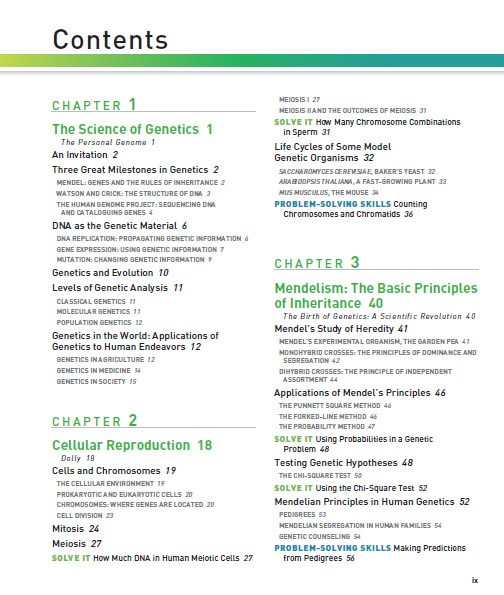
\includegraphics[width=0.5\textwidth]{contents01.png}}
\caption{Complex table of contents layout.}
\label{fig:toc}
\end{figure}


\begin{lstlisting}
\renewcommand\l@chapter[3]{%
  %#1 number and title  #2 page number
  \ifnum \c@tocdepth >\m@ne
    \addpenalty{-\@highpenalty}%
    \vskip 1.0em \@plus\p@
    \setlength\@tempdima{1.5em}%
    \begingroup
      \parindent \z@ \rightskip \@pnumwidth
      \parfillskip -\@pnumwidth
      \leavevmode
      \advance\leftskip\@tempdima
      \hskip -\leftskip
      \vbox{\raggedright#1\vskip1pt%
      \hrule width3cm height0.4pt}\par
      #2
      \penalty\@highpenalty
    \endgroup
  \fi}
\end{lstlisting}

\begin{lstlisting}
% define three parameters the chapter number, title separate
\renewcommand\l@chapter[3]{%
  %#1 number and title  #2 page number
  \ifnum \c@tocdepth >\m@ne
    \addpenalty{-\@highpenalty}%
    \vskip 1.0em \@plus\p@
    \setlength\@tempdima{1.5em}%
    \begingroup
      \parindent \z@ \rightskip \@pnumwidth
      \parfillskip -\@pnumwidth
      \leavevmode
      \advance\leftskip\@tempdima
      \hskip -\leftskip
      \vbox{\raggedright#1\vskip1pt%
      \hrule width3cm height0.4pt}\par
      #2
      \penalty\@highpenalty
    \endgroup
  \fi}
\cxset{chapter color=thegreen}
\l@chapter{\color{\chaptercolor@cx}\bfseries\chaptername\hskip1em\thechapter}{A Chapter Title}{12}
\end{lstlisting}


\subsection{Images in the TOC}
Figure \ref{fig:tocsteward} shows another |TOC| this time from a mathematics textbook. This is a much more complicated layout and includes images.

If we take a similarly flexible approach of redefining l@chapter we can try and format the toc shown in Figure \ref{fig:tocsteward}.

\begin{figure}[tp]
\centering

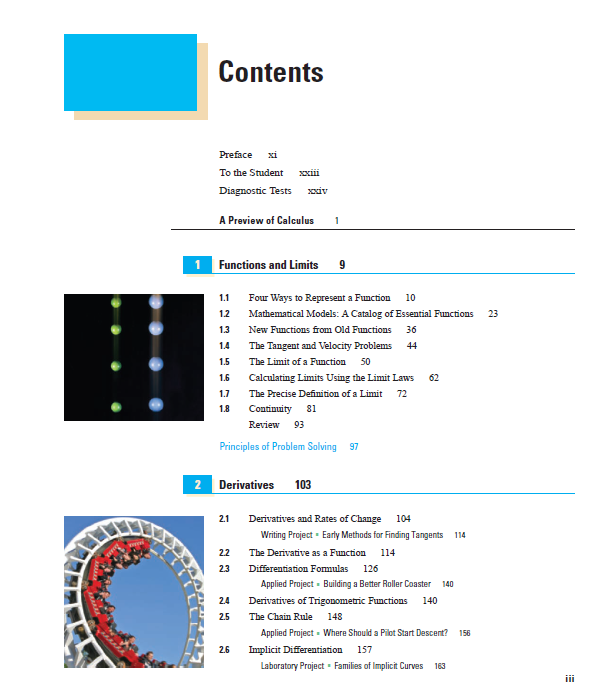
\includegraphics[width=0.8\textwidth]{contents02.png}
\caption{Complex table of contents layout.}
\label{fig:tocsteward}
\end{figure}



\begin{lstlisting}
\renewcommand\l@chapter[3]{%
  %#1 number and title  #2 page number
  \ifnum \c@tocdepth >\m@ne
    \addpenalty{-\@highpenalty}%
    \vskip 1.0em \@plus\p@
    \begingroup
      \parindent \z@
      \leavevmode
      \vbox{\raggedright\colorbox{blue}{\color{white}\bfseries\sffamily#1} #2\qquad  #3\vskip0pt%
      \color{blue}\hrule width0.7\textwidth height0.4pt}\par
      \penalty\@highpenalty
    \endgroup
  \fi}
\end{lstlisting}

\begin{lstlisting}
% define three parameters the chapter number, title separate
\cxset{
  toc chapter name/.store in=\chaptername,
  toc chapter name color/.code=\gdef\tocchapternamecolor@cx{#1},
  toc title color/.store in=\toctitlecolor@cx,
  toc title font-weight/.store in=\toctitlefontweight@cx,
  toc title before/.store in=\toctitlebefore@cx,
  toc title after/.store in=\toctitleafter@cx,
  toc after pagenumber/.store in=\tocafterpagenumber@cx,
}
\cxset{toc title color=theblue,  %interfers with links
       toc title font-weight=\fontfamily{ptm}\selectfont\bfseries ,
       toc title before=\hspace*{0.5em},
       toc title after=\hspace*{1.5em},
       toc after pagenumber=,
}

\renewcommand\l@chapter[3]{%
% #1 number #2
%  title  #2 page number
  \ifnum \c@tocdepth >\m@ne
    \addpenalty{-\@highpenalty}%
    \vskip 1.0em \@plus\p@
    \begingroup
      \parindent \z@
      \leavevmode
      \vbox{\raggedright\colorbox{blue}{\color{white}%
             \sffamily#1 }%
%% title formatting
        {\toctitlebefore@cx\color\toctitlecolor@cx\toctitlefontweight@cx%
          #2%
          \toctitleafter@cx}% font info
          #3\tocafterpagenumber@cx\vskip0pt%
              \color{blue}
              \hrule width0.7\textwidth height0.4pt}\par
      \penalty\@highpenalty
    \endgroup
  \fi}

\cxset{chapter color=thegreen}
\l@chapter{12}{A Chapter Title}{\thepage}%where is page number coming?numberline

\l@chapter{12}{A Chapter Title}{\thepage}
\end{lstlisting}


The above method of redefinition is a bit more flexible and can be extended to cover all cases that do not fall broadly with the standard class provisions. Any layout is possible.


\section{Writing the Table of Contents Entries}

So far we have examined the reading of the ToC file and next we need to understand the writing operation
to the ToC. If we have to ensure that information survives we need to write it to the file. This is done via two macros.




\begin{macro}{\addcontentsline}
The \cs{addcontentsline}\marg{table}\marg{type}\marg{entry} command allows the user to add an entry to a table of contents. The command adds the entry
\cs{contentsline}\marg{type}\marg{entry}\marg{page} to the \marg{.lot} file.
\end{macro}

\begin{teX}
 \addcontentsline{toc}{chapter}%
       {\protect\numberline{\thechapter}#1}
\end{teX}

\startlineat{144}
\begin{teX}       
 \long\def\addtocontents#1#2{%
 \protected@write\@auxout
 {\let\label\@gobble \let\index\@gobble \let\glossary\@gobble}%
 {\string\@writefile{#1}{#2}}}
\end{teX}

\begin{teX}
\def\addcontentsline#1#2#3{%
  \addtocontents{#1}{\protect\contentsline{#2}{#3}{\thepage}}}

\def\contentsline#1{\csname l@#1\endcsname}
\end{teX}

Of course the above are widely modified by the hyperref package and we should not touch them!


% \makeatletter\@specialfalse\@debugfalse\makeatother
\cxset{style13}
\cxset{title margin bottom=10pt}
\chapter{Introduction}
\addtocimage{-12pt}{-20pt}{../images/tocblock-fish.jpg}


\epigraph{``Begin at the beginning,'' the king said
"and then go on till you come to the end, then stop."}{
---Lewis Carroll, Alice in Wonderland}

\large

\noindent This package and its documentation attempts to eliminate some common 
problems encountered when using \LaTeX2e. The first one is the loading of 
recommended packages for a large and perhaps complicated document and 
the second is the re-designing of styles for a document.

 \LaTeX2e, does not provide a standard library, but comes equipped with
 a package mechanism that allows code extensions to be loaded as required.
 This has created a strong vibrant community, hundreds of packages and a 
 headache to both new and seasoned users. What packages are available, when
 to use them and in which order is a common theme for many questions on
 lists and |TX.SE|.

 It is quite common during the writing of a thesis or book
 for the author to keep on adding macros and packages
 at the preamble of the document. In most cases this can
 be satisfactory but in many others it leads to
 incompatibilities and errors. This package aims at
 minimizing one's preamble, by prefetching a number of
 commonly used packages. It also aims at loading them
 in the right order and providing patches for conflicts.
 
 I am hoping that using this package, will lead to less
 frustrations with the intricacies of \LaTeX2e\ packages.

The package code is complicated, but its usage is simple. You first load the package and then
you use one of the available templates:

 \begin{commands}[]{}
 \begin{verbatim}
 \usepackage{phd}
 \usetemplate{style13}
 \end{verbatim}
 \end{commands}

This is what you need to typeset a good looking book or thesis. The rest of this book is a footnote and you can skip them if you want. 

It will be better for the longer projects to just fork the
 package and adapt it to your needs. In this respect, I have
 uploaded the package to |github|.\footnote{\url{https://github.com/yannisl/phd}}

 My goal in selecting the packages and adding a number of 
 commands for the authors was to be able to typeset a 
 document for most common use cases, without the need of
 additional packages. The packages I selected are biased
 towards academic publications, although they can find use
 in almost any fields. The package provides a mechanism via
 PGF keys to provide a settings file. 
 
 Most of the documentation can be found in the implementation part.

Browse any books in a library or bookshop and the striking thing is that their design is very individualistic. They might have similarities but their main features vary. In many respects they resemble people's faces where minor differences have striking effects.

This package arose out of a question at stackexchange. How to redefine chapter heads. Having seen the popularity of the |pgf| package \cite{pkg-pgf} I realized that \latex users prefer this method of styling rather the traditional \latex method.

The user interface can be extended to basically all major packages. The principle is to keep to a minimum changes that can affect the LaTeX core commands. If there are any additions a key setting is provided to be able to revert back to normal LaTeX.

The workflow can be simplified. In addition I want to believe that the interface can provide a useful addition to the open source community and that other people will contribute style libraries, which will be simpler to write. It is also possible
to device an easy and uncomplicated web interface to handle
such a great number of variables.


Most people when they get started with \LaTeX\ will either use one of the standard classes such as the \docfile{book.cls} or one of the generic classes notably koma-script or memoir. Most students will be forced to use on of the many thesis classes available.

\section{The key value concept}

The key-value concept that originated with \LaTeX\ has been extended many times, the last and most serious implementation of it by Tantau in the PGF package. What essentially Tantau developed is a scripting language to script TeX code. The \tikzname and pgfplots packages are two major packaged that use keys effectively. Their popularity is growing and what this package does is to offer a user interface that has been modelled to be similar to that of \texttt{css} (cascade style sheets). 
\smallskip

\begin{scriptexample}{}{}
\textit{number} font-size = Large,\\
\textit{chapter} color = theblue
\end{scriptexample}
\smallskip

The main idea behind the package, is that you are configuring a document style by means of \emph{settings} rather than writing macros. In the example above the \emph{number, chapter} can be thought of as class or id names in css style sheets and the |font-size, color| as property settings that apply to the particular element. 


\subsection{Settings}

Settings are activated either by using the command |\cxset|  or by loading a full style sheet. In most cases you will probably import a style sheet and then modify some of the properties using |cxset|.  For example this heading has a dot after the subsection number. This was accomplished by setting,

We can de-activate it for the next and subsequent subsection headings with the setting:

\begin{scriptexample}{}{}
\begin{verbatim}
\cxset{subsection number after=\quad}
\end{verbatim}
\end{scriptexample}


\cxset{subsection number after=\quad,
          section number after=\quad,
          title margin bottom=10pt}
\renewsubsection

\subsection{Cascading}

Most values once set for a higher section will be seen in a cascade by all subsectioning commands in a similar fashion similar to CSS. These include properties such as color, font families and alignment. Best though to specify all of them for maximum flexibility to your users.

\section{On typography}

This package hopefully will assist in improving the typography of books set with \latexe. Any typographical comments on the various styles are just my own ramblingss and not necessarily absolute truths. Like fashion and art typography has opinions rather than absolute truths. In many styles the design is slightly adapted to blend a bit better with this manual. Also I did not select fonts as per the samples but this is left on you the user to decide.



\section{Packages and Fonts}

This manual has been typeset with numerous fonts in order to enable the typsetting of almost all the scripts provided by the Unicode standard. In order to process it from the |.dtx| file, these fonts must be available in your system, otherwise \XeLaTeX\ will have a problem finding the fonts and it will take an awful long time to process. This is especially true for the scripts section, where virtually all the Unicode defined scripts are discussed. You will need a fast computer and a fast hard disk to process the document within a reasonable time. When using \pkgname{fontspec} always define your fonts with the \cmd{\newfontfamily} this will speed up processing by an order of magnitude. Compiling from the command prompt will speed up compilation. Average speed 2-3 pages per second.

Many of \tex's parameters are stretched to the limit with a complicated document such as this manual. You will require a full distribution otherwise expect some errors. Important packages is \pkgname{morefloats} and \pkgname{morewrites}. The package will also expect that you have |e-tex| installed. Ubuntu users are normally one year behind in updates, so you might wish to update manually. It will take upwards of 5 minutes to compile fully on an old laptop and a couple of minutes on a state of the art computer.

The |dtx| should be processed best with its own make file provided for Windows only |phd.bat|. The make file will process the documentation using \lualatex. You can also process the document with \xelatex but is prone to produce errors. Using \latexe the sections on scripts etc will not be printed and a much shorter version of the manual is provided. 

\section{Scripts and Languages}

The package and the documentation offer a full repertoire of font selection keys for different scripts and languages. It hasn't been possible, however hard I tried to compile this section of the documentation with \xelatex, as it kept giving errors of too many files open. This was also not possible even with the \pkgname{morewrites} package loaded. With \lualatex the document compiled with no major problems other than the font rendering being of a lower quality to that of XeLaTeX om windows, other than disabling incompatible packages and a number of commands that were redefined. 

Some good news for multi-script typesetting is the Noto fonts from Google. These fonts named Noto from "No Tofu" meaning you do not see any little square blocks for undefined glyphs, are fast to load. Disantvantage you need to switch between font commands fairly often.

\section{This manual}

When developing the templates, I started using \emph{lorem ipsum} text as samples. Half-way through this
became a jumble mass of uninteresting pages interspersed with code. Headings and the contents of the book
determine both the structure and the selection of fonts, so I went back and wrote narratives  to accompany
the headings. Many of the narratives are semi-autobiographical in nature; others are clustered around books I read and my own interests. Some I stumbled on them accidentally and are mostly there to demonstrate some code.

Besides the templates and the code there is another narrative which is based on notes I kept on \tex and its friends over the years and are offered as a more advanced introduction to coding \latexe and \tex. The whole manual was typeset in a |ltxdoc| class, slightly modified to turn into a book class.

The implementation code is also available and it was mostly for my own benefit. The whole manual with the exception of the |\cxset| introduction, is just a test document. The notes and the “dissection” of the standard \latexe and the standard classes are there to explain the background to the many coding decisions that I took while I was developing the package.

PhD students are notorious for going in all directions and exploring many adjacent fields before they sit down and write their theses. Some become life-time students. To all these new men and women of the Renaissance that slave away to inch knowledge one thesis at a time, I dedicate this book and the name of the package.

 \section{Version control with Git and Github}
 
 If you are involved with code or a publication that will have frequent changes, you should consider
 some type of version control system. My own recommendation is to use |git| and an online repository such
 as |github|. The latter is currently very fashionable and makes sharing code easier. Note that the |github|
 offers both public as well as private repositories. The general recommendation is that for unpublished work
 such as a thesis or code under development, it is preferable to go for a private repository. 
 

 \section{Ordering of Packages}
 
One package that normally leads to errors is the 
\pkgname{hyperref}. The package which is an outstanding example of software engineering and supported single handledy by Heiko Oberdiek \citeyearpar{hyperref} redefines a a lot of internal commands of the kernel. As a lot of other packages do the same it has to be loaded at the end of the preable with the exception of some packages! 
 
 This manual is typeset according to the conventions of the
 \LaTeX \textsc{docstrip} utility which enables the automatic
 extraction of the \LaTeX{} macro source files~\cite{GOOSSENS94}.

 
 \href{http://tex.stackexchange.com/questions/96350/problem-with-algorithmic-and-hyperref}{problem with algorithmic and hyperref}

 \begin{verbatim}
\usepackage{float}  % load float package first!

\usepackage{hyperref} % let hyperref patch the float package stuff
.
 \usepackage{algorithm} % let algorithm use the patched version of the float package
 \end{verbatim}
 

\section{Known problems}

Perhaps the biggest issue with the package is the speed of
compilation with \XeLaTeX\ or \LuaTeX. This is to be expected, as both engines spend a lot of resources in font management. On demand loading of packages is something I have in the back of my mind. This should be done via document styles i.e., if a book is for the humanities, perhaps only a rudimentary amount of maths packages should be loaded.

\section{Future Directions}

\latexe and \tex usage appears to be increasing. This is mostly by programs that export results with \latexe code rather than authors writing books.  The method adopted here is easier to automate all sorts of reports and automated texts. I would like too develop a web interface for processing such templates and at the same time export into html instead of just producing pdfs. I have already a prototype.   

%\ClockFramefalse\ClockStyle=0\clock{13}{10}
%\ClockFramefalse\ClockStyle=1\clock{14}{22}
%\ClockFramefalse\ClockStyle=2\clock{15}{48}
%\ClockFramefalse\ClockStyle=3\clock{7}{50}
%
%\ClockFrametrue\ClockStyle=0\clock{11}{32}
%\ClockFrametrue\ClockStyle=1\clock{12}{0}
%\ClockFrametrue\ClockStyle=2\clock{8}{9}
%\ClockFrametrue\ClockStyle=3\clock{1}{15}

{\HHHUGE\showclock{0}{45}}











% \section{Introduction}
% 
% \LaTeX2e, does not provide a standard library, but comes equipped with
% a packagee mechanism that allows code extensions to be loaded as required.
% This has created a strong vibrant community, hundreds of packages and a 
% headache to both new and seasoned users. What packages are available, when
% to use them and in which order is a common theme for many questions on
% lists and |TX.SE|.
%
% It is quite common during the writing of a thesis or book
% for the author to keep on adding macros and packages
% at the preamble of the document. In most cases this can
% be satisfactory but in many others it leads to
% incompatibilities and errors. This package aims at
% minimizing one's preamble, by prefetching a number of
% commonly used packages. It also aims at loading them
% in the right order and providing patches for conflicts.
% 
% I am hoping that using this package, will lead to less
% frustrations with the intricacies of \LaTeX2e\ packages.
%
% Although I expect most users to just load the package, using
% the standard command:
%
% \begin{teX}
%  \usepackage{phd}
% \end{teX}
%
% it will be better for the longer projects to just fork the
% package and adapt it to your needs. In this respect, I have
% uploaded the package to |github|.
%
% My goal in selecting the packages and adding a number of 
% commands for the authors was to be able to typeset a 
% document for most common use cases, without the need of
% additional packages. The packages I selected are biased
% towards academic publications, although they can find use
% in almost any fields. The package provides a mechanism via
% PGF keys to provide a settings file. This in combination
% with the Athena package when it is made available will
% enable the creation of almost any publication, just by
% the use of a simple configuration file.
% 
% Most of the documentation can be found in the implementation part.
%
% 
% \section{Ordering of Packages}
% 
% One package that normally leads to errors is the 
% |hyperref|. As a lot of internal commands of the kernel
% and of some packages it has to be loaded at the end
% of the preable with the exception of some packages! 
% 
% This manual is typeset according to the conventions of the
% \LaTeX \textsc{docstrip} utility which enables the automatic
% extraction of the \LaTeX{} macro source files~\cite{GOOSSENS94}.
%
% 
% \href{http://tex.stackexchange.com/questions/96350/problem-with-algorithmic-and-hyperref}{problem with algorithmic and hyperref}
% \begin{verbatim}
%\usepackage{float}  % load float package first!
%
%\usepackage{hyperref} % let hyperref patch the float package stuff
%.
% \usepackage{algorithm} % let algorithm use the patched version of the float package
% \end{verbatim}
% \section{Conventions}
% \subsection{Defining Colors}
% All color definitions are of the form |the<color>|. So the setting for |theblue| is called
% |theblue|. This provides easy to remember commands.
% 
% \section{Document Structure}
% We do not load too many packages for document structure, a these are expected to be
% treated at class level.
% \begin{table}[ht]
% \centering
% \caption{Packages used for structure.}
% \begin{tabular}{ll}
%   \toprule
%   Package  & Default\\
%   \midrule
%   |multicol| & called by author  \\
%   \bottomrule
% \end{tabular}
% \end{table}
%
%
% \section{Version control with Git and Github}
% If you are involved with code or a publication that will have frequent changes, you should consider
% some type of version control system. My own recommendation is to use |git| and an online repository such
% as |github|. The latter is currently very fashionable and makes sharing code easier. Note that the |github|
% offers both public as well as private repositories. The general recommendation is that for unpublished work
% such as a thesis or code under development, it is preferable to go for a private repository. 
% 
% \subsection*{What is the difference between Git and GitHub?}
%git is a version control, system think of it as a series of snapshots (commits) of your code. You see 
%a path of this snapshots, in which order they where created. You can make branches to experiment and come back to snapshots you took.
%GitHub, is a web-page on which you can publish your git repositories and collaborate with other people.
%
% \subsection*{Is git saving every repository locally (in the user's machine) and in GitHub?}
%
% No, it's only local. You can decide to push (publish) some branches on GitHub.
%
% \subsection*{Can you use Git without GitHub? If yes, what would be the benefit for using GitHub?}
%
% Yes, it runs local. You could back it up with dropbox. See also \href{http://dotmonster.co/backup-and-sync-folders-with-dropbox-and-symbolic-links/}{how to sync your git folders to dropbox}.
%
%\subsection*{How does Git compare to a backup system such as Time Machine?}
%
%It's a different thing, git lets you track changes and your development process. If you use git with GitHub, it becomes effectively a backup. However usually you would not push all the time to GitHub, at which point you do not have a full backup if things go wrong. I use git in a folder that is synchronized with dropbox.
%
% To synchronize the two, you create a symlink in your Git folder, i.e., in your repository. This can even be done in windows although it is normally called a \textit{short-cut}. Write click in the folder and create a short-cut to the drop-box folder. For example if you create a folder \texttt{pic} to hold your pictures, this folder will be automatically uploaded at \texttt{dropbox}. You don't want your pictures tracked at Github, as they do not really need version control. Do not forget to exclude them by typing in the \texttt{.gitignore} file the directive  \verb|*.lnk|.
%
%\subsection*{Is this a manual process, in other words if you don't commit you wont have a new version of the changes made?}
%
%Yes, commiting and pushing are both manual.
%
%\subsection*{If are not collaborating and you are already using a backup system why would you use Git?}
%
% You program worked. You developed more, your program does not work. git diff, shows you the difference between the current code and the last working commit.
%
% Or you just go back to the last working. You want to try a change, but are not sure it really will work. 
% You create a branch, test you code change. If it works fine, you merge it to the main branch. If it does not you throw the branch away and go back to the main branch.
% You did some debugging. Before you commit you always look at the changes from the last commit. You see your debug print statement that you forgot to delete.
%
%Make sure you check gitimmersion.com.
% 
% \StopEventually{}
%
%
%<*package>
%
% \cxset{style13}
% \cxset{section align=left,
%        section color=teal,
%         section font-weight=bold,
%         title font-family=sfamily,
%         title font-shape=upshape,
%         subsection indent=0pt,
%          subsection font-shape=upshape}
% \renewsubsection
%
% \thispagestyle{headings}
%
% \chapter{Implementation}
%
% \section{Preliminaries}
%
%    Standard file identification. We first announce the package and require that 
%    it be used with LaTeX2e. 
%    \begin{macrocode}
\NeedsTeXFormat{LaTeX2e}
[1994/12/01]%
\ProvidesPackage{phd}[2013/2/26 v1.0 less preamble (YL)]%
%    \end{macrocode}
% 
%
% \section{Package Management} 
%  
% In order to keep track of all the packages and keys we require a
% number of macros will be defined first.
% 
% Each of the packages used by this document is loaded conditionally.
% However, it might be nice to know if we have a complete set.  So we
% define |\ifcomplete| which starts true, but gets set to false if any
% package is missing. Some code is necessary in order to manage 
% the complexity.
% I am idebted to the source of |symbols.tex| for some of the macros.
% There are a number of symbols (e.g., \cmd{\Square}) that are defined by      
% multiple packages.  In order to typeset all the variants in this       
% document, we have to give glyph a unique name.  To do that, we define  
% \cs{savesymbol{XXX}}, which renames a symbol from \cs{XXX} to \cmd{origXXX}, and    
% \cmd{restoresymbols{yyy}{XXX}}, which renames \cmd{origXXX} back to \cmd{XXX} and     
% defines a new command, |\yyyXXX|, which corresponds to the most recently 
% loaded version of |\XXX|.                                                
%                                                                        
% This implementation of \savesymbol and \restoresymbol was copied from  
% the |savesym| package, which started with symbol.tex's old definitions   
% of those macros and improved upon them.  However, \renamerobustsymbol  
% and |\ifnotsavedsym| are new to this set.                                
%                                                                        
% Save a symbol that we know is going to get redefined.
%
% \begin{macro}{\savesymbol}
%    \begin{macrocode}
\newcommand*{\savesymbol}[1]{%
  \expandafter\let\csname orig#1\expandafter\endcsname\csname#1\endcsname
  \expandafter\let\csname #1\endcsname\relax
}
%    \end{macrocode}
% \end{macro}
%    
% Restore a previously saved symbol, and rename the current one.
%    \begin{macrocode}
\newcommand*{\restoresymbol}[2]{%
  \expandafter\global\expandafter\let\csname#1#2\expandafter\endcsname%
    \csname#2\endcsname
  \expandafter\global\expandafter\let\csname#2\expandafter\endcsname%
    \csname orig#2\endcsname
}
%    \end{macrocode}   
% Rename a robust command.
%    \begin{macrocode}
\newcommand*{\renamerobustsymbol}[2]{%
  \expandafter\let\expandafter\origrealcommand
    \csname #2\space\endcsname
  \expandafter\global\expandafter\let\csname#1#2\endcsname=\origrealcommand
}
%    \end{macrocode}
% Test if a symbol is not saved.
%    \begin{macrocode}
\def\ifnotsavedsym@helper#1#2!{\expandafter\ifx\csname orig#2\endcsname\relax}
\newcommand*{\ifnotsavedsym}[1]{%
  \expandafter\ifnotsavedsym@helper\string#1!%
}
%    \end{macrocode}
% \begin{macro}{\ifcomplete}
%    \begin{macrocode}
\newif\ifcomplete
%    \end{macrocode}
% \end{macro}    
%    
% For debugging purposes we define a switch that enables us to toggle
% on and off the loading of packages.
% 
%    \begin{macrocode}
\newif\ifloadpackages
\loadpackagestrue
%    \end{macrocode}
%    
% |\IfStyFileExists*| is just like |\IfFileExists|, except that it appends
% ".sty" to its first argument.  |\IfStyFileExists| is the same as
% |\IfStyFileExists*|, but it additionally adds its first argument to a list
% (|\missingpkgs|) and marks the document as incomplete (with
% |\completefalse|) if the |.sty| file doesn't exist.
% 
% \begin{macro}{\missingpkgs}
% \begin{macro}{\foundpkgs}
%   \begin{macrocode}
\newcommand{\missingpkgs}{}
\newcommand{\foundpkgs}{}
\newcommand{\if@sty@file@exists@star}[3]{%
  \ifloadpackages
    \IfFileExists{#1.sty}{#2}{#3}%
  \else
    #3%
  \fi
}
\newcommand{\if@sty@file@exists}[3]{%
  \ifloadpackages
    \IfFileExists{#1.sty}%
                 {#2\@cons\foundpkgs{{#1}}}%
                 {#3\completefalse\@cons\missingpkgs{{#1}}}%
  \else
    #3\completefalse\@cons\missingpkgs{{#1}}%
  \fi
}
\newcommand{\IfStyFileExists}{%
  \@ifstar{\if@sty@file@exists@star}{\if@sty@file@exists}%
}
%    \end{macrocode}
% \end{macro}
% \end{macro}
% \subsection{Utility macros for displaying symbols and fonts}
% \subsubsection{Other}
% \subsubsection{More}
%
% In the sections that follow, we use a number of utilities for
% displaying fonts and utilities in tables and figures, we collect
% them here and make them available to the user for document
% use.
%
%    \begin{macrocode}
% From stmarysrd symbols package
% A very convenient command to typeset symbols.
% Much preferable than tables. Slight modifications to
% make it a bit more clear
\def\symbols{\flushleft}
\def\endsymbols{\endflushleft}
\def\dosymbol#1{%
   \leavevmode\hbox to .33\textwidth{%
    \hbox to 1.2em%
    {\hss$#1$\hfil}%
   \footnotesize\texttt{\string#1}\hss}%
   \penalty10}
%    \end{macrocode}
%
% \symbols
% \dosymbol{\Square} \dosymbol{\square} \dosymbol{\Diamond} \dosymbol{\diamond} \(\dosymbol{\symbol{60}}\)
% \endsymbols
%   
% \section{Best practices} 
% 
% We load a few packages for fixes and errors and |nag| if outdated packages are used.
% Modify to suit your requirements.  
% Package management is a bit complex to avoid errors
% with options.
%To find out if a package has already been loaded, use
%|\@ifpackageloaded|\meta{package}\meta{true}\meta{false}.
%|\@ifpackagelater| To find out if a package has already been loaded with a version more recent
%|\@ifclasslater| than version, use |\@ifpackagelater|\meta{hpackagei}\meta{hversioni}\meta{true}\meta{hfalsei}.
%|\@ifpackagewith| To find out if a package has already been loaded with at least the options
%hoptionsi, use |\@ifpackagewith|\meta{hpackagei}\meta{hoptionsi}\meta{htruei}\meta{hfalsei}. 
%There exists one package that can't be tested with the above commands: the
%fontenc package pretends that it was never loaded to allow for repeated reloading
%with different options (see ltoutenc.dtx for details).
%
% \subsection{Best Practices}
% 
% We include the following two packages to provide the standard fixes
% for \LaTeX2e\ and the |nag| package to provide some guidance as to good
% practices. We set the |nag| keys to |orthodox| and |l2tabu.|
% \url{http://tex.stackexchange.com/questions/19264/techniques-and-packages-to-keep-up-with-good-practices?rq=1}
% and \href{http://stackoverflow.com/questions/193298/best-practices-in-latex}{best practices in LaTeX.}
%    \begin{macrocode}
\RequirePackage{fixltx2e}                % LaTeX2e fixes
%    \end{macrocode}
%
% We load pgfkeys for key management.
% 
%    \begin{macrocode}
\RequirePackage{etex}
\RequirePackage{pgf,pgfkeys}               % before onlyasmath
\def\cx@optionlist{}
\def\cxuselibrary#1{\cxset{library/.cd,#1}}
%
% The library is added by inputting the file and setting the path accordingly.
\def\cx@add@library#1#2{%
  \cxset{library/#1/.code={\@ifundefined{cxlibrary@#1@loaded}{\input #2}{}}}%
  \DeclareOption{#1}{\edef\cx@optionlist{\cx@optionlist,#1}}%
}
\pgfkeys{/chapter/.is family}
\newcommand\cxset{\pgfqkeys{/chapter }} %Notice this is pgf q keys
%
%

\cxset{nag keys/.store in =\nagkeys@cx,
       onlyamsmath keys/.store in=\onlyamsmathkeys@cx,
       xcolor keys/.store in=\xcolorkeys@cx}
%        
%
%%
%% This is file `settings.tex',
%% generated with the docstrip utility.
%%
%% The original source files were:
%%
%% phd.dtx  (with options: `settings')
%% ----------------------------------------------------------------
%% phd --- A package to beautify documents.
%% E-mail: yannislaz@gmail.com
%% Released under the LaTeX Project Public License v1.3c or later
%% See http://www.latex-project.org/lppl.txt
%% ----------------------------------------------------------------
%% 








%% Some settings
\cxset{nag keys = {l2tabu,%
                   orthodox}}
\cxset{onlyamsmath keys = {warning}}

\endinput
%%
%% End of file `settings.tex'.
 % experimental
%\cxset{nag keys = {l2tabu,%
%                   orthodox,%
%                   %
%                  }}
%    \end{macrocode}
%
% \begin{macro}{xcolor}
% 	For |xcolor| we try and load as many pre-defined colornames as
% 	possible.
%    \begin{macrocode}
\cxset{xcolor keys={fixpdftex,xtable,usenames,dvipsnames,
                    svgnames,x11names}}                     
% Set amsmath keys
%
%    \end{macrocode}
% \end{macro}
%
%    \begin{macrocode}
\PassOptionsToPackage{\nagkeys@cx}{nag}
\RequirePackage{nag}   
%    \end{macrocode}
%
%
% \begin{macro}{onlyasmath}
% The package |onlyasmath| also provides errors for deprecated math
% commands like using |$$|\ldots|$$| which can result in unwanted spaces
% being introduced in the typsetting of the document. The recommended 
% way is to use |\[|\ldots|\]|. The package was developed by Harold Harders
% and although targetted for class writers one might as well use it directly.
% 
%    \begin{macrocode}

\PassOptionsToPackage{\onlyamsmathkeys@cx}{onlyamsmath}
\RequirePackage{onlyamsmath} 
\RequirePackage{microtype}
%    \end{macrocode}
% \end{macro}
%
% I prefer to issue an error rather than a warning to instill good
% practices early during document processing.
% 
% 
% \subsection{Graphics}
% 
% We load the package |graphicx| with no options. We let |graphicx|, to 
% handle any draft options via the class itself. We load the package |caption|
% for any captions outside floats. (Needs checking where to place).
% \href{http://tex.stackexchange.com/questions/3131/graphicspath-for-miktex}{graphicspath for MikTeX} check
% adds figures etc to paths. We add some common paths. If you call your image
% folders |image| or |graphics| you don't need to do anything else.
% 
%    \begin{macrocode}
\RequirePackage{graphicx}
\setkeys{Gin}{width=\linewidth,totalheight=\textheight,keepaspectratio}
\graphicspath{{graphics/}{graphics//}{images//}{./graphics/}{../graphics/}{./pic/}{../pic}}
\RequirePackage{wrapfig}
%    \end{macrocode} 
%
% \begin{macro}{rotating}
% The package performs
% most sorts of rotation one might like, including rotation of complete floating
% figures and tables. The package was developed by Robin Fairbairns
% Sebastian Rahtz and Leonor Barroca. We use the option |quiet| as the 
% package is rather verbose.
%
%    \begin{macrocode}
\RequirePackage[quiet]{rotating}
%    \end{macrocode} 
% \end{macro}
% 
% \section{Color Management}
%
% Most classes load the |xcolor| package. Including
% it here, should either be able to check if it was 
% loaded by the class or to pass the options before
% the class itself. This package is a common source
% of errors, as classes load it with mostly different options.
% Because of this is also a good example to test our code
% in a number of minimal working examples.
%
%    \begin{macrocode}
\@ifpackageloaded{xcolor}{}%
 {\PassOptionsToPackage{\xcolorkeys@cx}{xcolor}
  \RequirePackage{xcolor}}
%    \end{macrocode}
%
%	We adopt the convention that colour names used in code should be
%	prefixed by a |the|. For simplicity we also adopt the convention
%    that all colours defined in colour schemes should be in lowercase
%	(less keystrokes and matches the styles of |pgf| keys). 
%
%    \begin{macrocode}
\definecolor{theblue} {rgb}{0.02,0.04,0.48}
\definecolor{thered}  {rgb}{0.65,0.04,0.07}
\definecolor{thegreen}{rgb}{0.06,0.44,0.08}
\definecolor{thelightgreen}{rgb}{0.06,0.44,0.06}
\definecolor{thegrey} {gray}{0.5}
\definecolor{thegray} {gray}{0.5}
\definecolor{thedarkgray} {gray}{0.95}
\definecolor{lightgray}{gray}{0.6}
\definecolor{thelightgray}{gray}{0.6}
\definecolor{theshade}{gray}{0.94}
\definecolor{theframe}{gray}{0.75}
\definecolor{thecream}{rgb}{1,0.95,0.4}
\definecolor{spot}{rgb}{0,0.2,0.6}
\definecolor{boxframe}{gray}{0.8}
\definecolor{boxfill}{rgb}{0.95,0.95,0.99}
\definecolor{theoption}{rgb}{0.118,0.546,0.222}
\definecolor{themacro}{rgb}{0.784,0.06,0.176}
\definecolor{ExampleFrame}{rgb}{0.628,0.705,0.942}
\definecolor{ExampleBack}{rgb}{0.963,0.971,0.994}
\definecolor{Hyperlink}{rgb}{0.281,0.275,0.485}
\colorlet{thehyperlink}{theblue}
\newcommand*{\defaultcolor}{\color{black}}
\newcommand*{\spotcolor}{\color{spot}}
%    \end{macrocode}
% 
%    \begin{macrocode}
\newcommand{\done}{\cellcolor{teal}done}  
\newcommand{\partialdone}{\cellcolor{yellow}done}
\newcommand{\hcyan}[1]{{\color{teal} #1}}
%    \end{macrocode}
%
% \section{Rules}
%
% \begin{macro}{\thickrule}
% \begin{macro}{\thinrule}
% \begin{macro}{\mediumrule}
%	We will use later on different styles of rules to decorate chapter headings.
%	We define a few here to simplify code later on.
%
%    \begin{macrocode}
\DeclareRobustCommand\thickrule{\leavevmode \leaders \hrule height 3pt \hfill \kern \z@}
\DeclareRobustCommand\thinrule{\rule{\textwidth}{0.4pt}}
\DeclareRobustCommand\mediumrule{\rule{\textwidth}{0.8pt}}
%    Adjusted to get toc parameters in
\DeclareRobustCommand\Rule{{\color{\tocchapternumberfill@cx}\rule[-4.1pt]{13cm}{0.4pt}}}
\DeclareRobustCommand\bottomline{\medskip
   \noindent\rule{\linewidth}{0.4pt}\medskip}
\DeclareRobustCommand\topline{\par\medskip
 \noindent\rule{\linewidth}{0.4pt}\medskip} 
%    \end{macrocode}
% \end{macro}
% \end{macro}
% \end{macro}

%
% \section{Filler Text}
%
%
% \begin{macro}{lipsum}
% 	publishing and graphic design, lorem ipsum is placeholder text (filler text) 
% 	commonly used to demonstrate the graphics elements of a document or visual 
% 	presentation, such as font, typography, and layout, by removing the distraction 
% 	of meaningful content. The lorem ipsum text is typically a section of a Latin text 
% 	by Cicero with words altered, added and removed that make it nonsensical in meaning 
% 	and not proper Latin. Other packages exist such as |kantlipsum| and |blindtext|, 
% 	however, both result in somewhat legible texts, which defeats the purpose of 
% 	providing texts that the reader is not going to read. the extensions |lipsumx| 
% 	aim at providing a gap between the three packages. It provides extensions
% 	for full document testing.
%    \begin{macrocode}
\newif\ifLIPSUM
\RequirePackage{lipsum}
\RequirePackage{kantlipsum}
\RequirePackage{blindtext}
%    \end{macrocode}
% \end{macro}
%
% 
% \begin{macro}{\lorem} 
%	We declare a short macro \cs{lorem} to be used for testing, as well as 
%	testing captions and the like.
%    \begin{macrocode}
\DeclareRobustCommand\lorem{Fusce adipiscing justo nec ante. Nullam in enim.
 Pellentesque felis orci, sagittis ac, malesuada et, facilisis in,
 ligula. Nunc non magna sit amet mi aliquam dictum. In mi. Curabitur
 sollicitudin justo sed quam et quadd. \par}
%    \end{macrocode}
% \end{macro}
%
%
% \section{Tables}
% 
% \begin{macro}{\booktabs}
% \begin{macro}{\inc}
% \begin{macro}{\resetinc}
% 	It is unlikely that a publication, would not have a table
% 	somewhere, to make life easier we load Simon Fear's |booktabs|. The manual is a must
% read if you want to typeset typographically attractive tables.\footnote{Notice I haven't said
% typographically correct, there is no such thing.} We don't need to set any keys for the
% package.
%
%    \begin{macrocode}
\RequirePackage{booktabs}
\newcounter{step}
\def\resetinc{\setcounter{step}{0}}
\def\inc{\stepcounter{step}\thestep}
%    \end{macrocode}
% \end{macro}
% \end{macro}
% \end{macro}
%
%
% \begin{macro}{tabularx}
% This package by David Carlisle's enables the typesetting of fixed width 
% tables and can stretch
% specific columns. The package loads the |array| package, but we save it from some
% trouble by pre-loading it first, so we can capture its loading. The package has two keys
% |infoshow| and |debugshow| which we don't bother at this stage to load.
% 
%    \begin{macrocode}
\RequirePackage{tabularx}
%    \end{macrocode}
% \end{macro}
%
% \begin{macro}{array}
% \begin{macro}{delarray}
% The addition to array.sty added in delarray.sty is a system of implicit |\left|
%|\right| pairs. If you want an array surrounded by parentheses, you can enter:
%|\begin{array}({cc}) . .|
% 
%    \begin{macrocode}
% \RequirePackage{delarray} gives problems
\RequirePackage{array}
%    \end{macrocode}
% \end{macro}
% \end{macro}
%
% \begin{macro}{dcolumn}
% The |dcolumn| package also by David Carlisle is loaded next. This package 
% defines a system for defining columns of entries in an |array|
% or tabular which are to be aligned on a `decimal point'. It also loads the |array|
% package, which we have already loaded.
% 
%    \begin{macrocode}
\RequirePackage{dcolumn}
%    \end{macrocode}
% \end{macro}
%
% \begin{macro}{longtable}
% 
% Perhaps the |longtable| package, needs no introduction. It has some
% peculiar settings and sometimes a couple of runs before it settles
% down. The package has four keys |errorshow|, |pausing|, |set| and |final| looks 
% as if they deprecated, at this stage we make onlty a mental note of it.
% The package cannot be used within |multicolumn| environments and will
% emit an error. 
% 
%    \begin{macrocode}
\RequirePackage{longtable}
%    \end{macrocode}
% \end{macro}   
%
% \begin{macro}{multirow}
% 
% The |multirow| by Piet van Oostrum and its two companion packages
% |bigdelim| and |bigstrut| can be used to define multirow cells. They are difficult
% to get right and in most instances one can redesign the tables better without
% resorting to multi-rows. It has a strange interaction with the |colortbl|
% and a hack around its usage which we will load next.
% 
%    \begin{macrocode}
\RequirePackage{colortbl}
\RequirePackage{multirow}
%    \end{macrocode}
% \end{macro}
% 
% \begin{macro}{threeparttable}
% This package by Donal Arsenau facilitates tables with titles (captions) and notes. The
% package comes with a number of options |para|, |flushleft|, online and normal.
%    \begin{macrocode}
\RequirePackage{threeparttable}
%    \end{macrocode}
% \end{macro}
%
%  {\begin{center}
%
%  \begin{threeparttable}[b]
%    \caption{...}
%  \begin{tabular}{ll} 
%   \toprule
%    one cell 42\tnote{1}&\\
%    another cell \tnote[2]&\\
%  \bottomrule
%  \end{tabular}
%  \begin{tablenotes}
%    \item [1] the first note ...
%    \item [2] the second note
%  \end{tablenotes}
%  \end{threeparttable}
%  \end{center}}
%  
% \section{Landscape Pages}
%
% A common request from authors is to rotate text, tables and or
% figures and to typeset the content using a landscape page.
%
% \begin{macro}{pdflscape}
% \begin{macro}{lscape}
% This package by Heiko Oberdiek Package |pdflscape| adds PDF support 
% to the environment landscape 
% of  package |lscape| by setting the PDF page attribute /Rotate. 
% It has to be loaded after |lscape| so we let it load it itself.
%
%    \begin{macrocode}
\RequirePackage{pdflscape}
%    \end{macrocode}
% \end{macro}
% \end{macro}
%  
% \section{Maths}
%
% 	Although we cognisant that there are documents that do not use math
% 	and perhaps others that our selection of packages is inadequate, we
% 	offer a bundle of what we think will cover most of the cases. One
% 	issue with maths is that we are limited with TeX's built-in math
% 	alphabet limitations.
% 
% \begin{macro}{empheq}
% \begin{macro}{mathtools} 
%	We start with |mathtools|\ctan{mathtools}, as it loads the
% 	|amsmath| package and can also pass options to it. The package was developed 
% 	by LarsMadsen and is maintained by Will Robertson and Joseph Wright. It
% 	appears to be very popular with a lot of scholars in the sciences and
% 	mathematical fields and hence I decided to  include it here.
% 
%    \begin{macrocode}
\RequirePackage[allowspaces]{empheq} %defines harpoon macros
\PassOptionsToPackage{leqno}{mathtools}
\RequirePackage{mathtools}
\RequirePackage{nicefrac}
%    \end{macrocode}
% \end{macro}
% \end{macro}
%
% Many of the tools shown in this manual can be turned on and off by 
% setting a switch to
% either true or false. In all cases it is done with the command 
% |\mathtoolsset|. A typical
%  use could be something like
% \begin{equation}
%  a=c+d
% \end{equation}
%
% This provides a useful way to hook into the package options
% using our setting interface.
%
%    \begin{macrocode}
\cxset{tag left bracket/.store in = \leftbracket@cx,
       tag right bracket/.store in = \rightbracket@cx,
       tag font-weight/.store in = \tagfontweight@cx,
       mathtool center colon/.store in=\centeredcolon@cx}
%
\cxset{tag left bracket =[,
       tag right bracket =],
       tag font-weight=\textbf,
       mathtool center colon=false} 

\newtagform{brackets}[\tagfontweight@cx]{\leftbracket@cx}%
           {\rightbracket@cx}
\mathtoolsset{centercolon=true,mathic}%italic correction in math
\numberwithin{equation}{section}
%    \end{macrocode}
%
% \[ a:= z+i\]
% \mathtoolsset{centercolon=false}
% \[ a:= z+i\]
%  \usetagform{brackets}
%  \begin{equation}
%   a = b +c
%  \end{equation}
% 
% Test \mbox{{\Huge\WomanFace  \Checkedbox \Square}}
%  $\Delta$ 
%
%    \begin{macrocode}
\RequirePackage{amssymb}[2002/01/22]
\RequirePackage{amsthm}[2002/01/22]
\RequirePackage{amsopn}
\RequirePackage{amscd}
\RequirePackage{accents}
\RequirePackage{dsfont}
%    \end{macrocode}
% The package |stmaryrd| can be used for additional symbols. 
%    \begin{macrocode}
%\RequirePackage{stmaryrd}
%    \end{macrocode}
% 
% The \package{amscd} is probably not useful at all as people are
% moving to graphical programs such as TikZ for their commutative
% diagrams.
%  
% \begin{macro}{empheq} 
%    \begin{macrocode}
\RequirePackage{empheq}
%    \end{macrocode}
% \end{macro}
%
%This package\footnote{The package is part of the \texttt{mh}-bundle 
%of Morten H\o gholm (\href{http://www.ctan.org/tex-archive/macros/latex/contrib/mh/}{CTAN://macros/latex/contrib/mh/}).} 
%supports different frames for math environments of the AmSmath
%package. It doesn't support  all the environments from standard \LaTeX{} which 
%are not modified by \AmSmath.
%
%With the optional argument of the empheq
%the preferred box type
%can be specified. A simple one is |fbox|.
%
%\begin{empheq}[box=\fbox]{align}
%	f(x)=\int_1^{\infty}\frac{1}{x^2}\,\mathrm{d}x=1
%\end{empheq}

% \subsection{xpfeil}
% The package |extpfeil| loads |stmaryd| with limited options
% we temporarily make |RequirePckage| a no-op to prevent
% LaTeX from complaining.
% 
%    \begin{macrocode}   
\newif\ifXPFEIL
\newcommand\XPFEIL{\pkgname{extpfeil}}
\IfStyFileExists{extpfeil}
  {\XPFEILtrue
   % extpfeil tries to do a \RequirePackage of stmaryrd with
   % conflicting options from what we used to load stmaryd.  We
   % therefore temporarily make \RequirePackage a no-op to prevent LaTeX
   % from complaining.
   \let\origRequirePackage=\RequirePackage
   \renewcommand*{\RequirePackage}[2][]{}
   \savesymbol{xlongequal}
   \savesymbol{xmapsto}
   \RequirePackage{extpfeil}
   \restoresymbol{XPFEIL}{xlongequal}
   \restoresymbol{XPFEIL}{xmapsto}
   \let\RequirePackage=\origRequirePackage
  }
  {}
%    \end{macrocode}
%      
% For calligraphic fonts we load the package |eucal|. The package 
% is not actually needed, if 
% amsfonts are loaded? Consider removing.
%    \begin{macrocode}
\newif\ifEU
\IfStyFileExists{euscript}
  {\EUtrue\RequirePackage[mathcal]{euscript}
   \renewcommand{\mathcal}[1]{\mbox{\usefont{U}{eus}{m}{n}##1}}
  }
  {\let\CMcal\mathcal}
\RequirePackage{bm}
\RequirePackage{bbm}

%    \end{macrocode}
%
%
% \begin{macro}{upgreek} This package by Walter Schmidt provides fonts
% and commands for an upright Greek alphabet. It makes the upright
% Greek characters from the `Euler'  or `Adobe Symbol' typefaces avaialable as 
% math symbols. It defaults to the Euler option. The package offers three
% options |Euler|, |Symbol| and |Symbolsmallscale|.
% 
%    \begin{macrocode}
\newif\ifUPGR
\RequirePackage[Symbol]{upgreek}
%    \end{macrocode}
% \end{macro}
%
% \[
%  \begin{array}{lll}
%   \upalpha  &\upbeta    &\upgamma\\ 
%   \updelta  &\upepsilon &\upzeta\\
%   \upeta    &\uptheta   &\upiota \\
%   \upkappa &\uplambda   &\upmu\\
%   \upnu    &\upxi      &\uppi\\
%   \uprho    &\upsigma  &\uptau\\
%   \upupsilon &\upphi   &\upchi\\
%   \uppsi     &\upomega  &\upvarepsilon\\
%   \upvartheta &\upvarpi  &\\
%  \end{array}
% \]
%
% 
% 
% \section{Special Symbols}
%
% The next section of the package, deals exclusively for packages that
% handle symbols. The best guide to such symbols is 
% \textit{The Comprehensive LaTeX Symbols Guide}. One needs to distinguish
% a number of different types of symbols required for a manual and it is
% a difficult exercise to make a selection. Another issue with symbols
% is that there is a bit of overlap between the various fonts and commands
% as to be expected.
%\subsection{Symbols in textcomp}
%, has numerous symbols \ldots
% We use the \pkg{texcomp} package for special symbols, such as |\checkmark|
%  \( \mho \Diamond \leadsto \rhd \diamond \Diamond \). The sort of the standard package
% latexsym is not loaded as it duplicates functionality of the if one makes use of the packages |amsfonts| or |amssymb|.
%
% \begin{macro}{textcomp} 
% \begin{macro}{mathcomp} The package |textcomp| is part of the \LaTeX2e
% distribution. The description of the package
% on ctan can give the erroneous idea that it is obsolotet, on the contracry % is part of the original distribution.textcomp is not obsolete, it's just not distributed as extra package any more since it's distributed with the basic LaTeX. The mathcomp package defines macros for using some of these text... symbols with math and the abbreviation tc...
%
%  The symbols are used by calling them by their name. E.g. \textleaf:
%  \verb|\textleaf|.
%  
%  In mathematics the package \verb|mathcomp| works. Then the prefix
%  \verb|text| is replaced by \verb|tc|, for \emph{t}ext\emph{c}omp:
%  |tcohm|  \( \tcohm \)
% 
% The |mathcomp| package takes one option to describe the
% font to be used. We use |rmdfault| as teh option to default to
% the \cs{rmdefault} font.
% 
%    \begin{macrocode}
\RequirePackage{textcomp}
\PassOptionsToPackage{mathcomp}{rmdefault}
\RequirePackage{mathcomp}
%    \end{macrocode}
% \end{macro}
% \end{macro}
%
% \begin{macro}{exscale}
%
%
%This package implements scaling of the math extension font |cmex|. If this package is used the site needs scaled versions of the font |cmex10| in the sizes 10.95pt, 12pt, 14.4pt, 17.28pt, 20.74pt, and 24.88pt (corresponding to standard magsteps using |\magstephalf|, and |\magstep1| through |\magstep5|). Additionally |cmex| variants for the sizes |7pt| to 9pt are necessary. These fonts are part of the AMS font pack­age.
%
% 
%
%    \begin{macrocode}
\RequirePackage{exscale}
\RequirePackage{relsize}
%    \end{macrocode}
% \end{macro}
%
% An example to scale math using the exscale package. Perhaps for
% using slides etc.
%
%\begin{minipage}[c]{1.0\textwidth}%
%\centering\large\[
%\int_{-1}^{+1}\frac{f(x)}{\sqrt{1-x^{2}}}\,\mathrm{d}x\approx\frac{\pi}{n}%
%\sum_{i=1}^{n}f\left(\cos\left(\frac{2i-1}{2n}\right)\right)\]
%\end{minipage}%
%
% \begin{macro}{\tabitem} The \package{textcomp} 
% provides a nice helper macro for typesetting symbols in normal, bold
% and italics. I must think of a more semantic name than |tabitem|.
%
%    \begin{macrocode}
\newcommand{\tabitem}[2]{%
  \texttt{\symbol{`\\}#1} & \@nameuse{#1} 
   & \bfseries\@nameuse{#1}& \itshape\@nameuse{#1}
   \ifthenelse{\equal{#2}{}}
    {}
    {& \texttt{\symbol{`\\}#2} & \@nameuse{#2} 
     & \bfseries\@nameuse{#2}
     & \itshape\@nameuse{#2} \\}
}
%    \end{macrocode}
% \end{macro}
%

%\setlength{\LTleft}{0pt}%
%\setlength{\LTright}{0pt}
%\noindent
%\begin{longtable}{%
%    @{}ll@{}l@{}l@{\extracolsep{\fill}}l!{\extracolsep{0pt}}l@{}l@{}l@{}}
%  \multicolumn{4}{c}{\textbf{Symbol}} & 
%  \multicolumn{4}{c}{\textbf{Symbol}} \\ 
%  \midrule
%\endhead
%
%%  \tabitem{textcapitalcompwordmark}{textascendercompwordmark}
%  \tabitem{textquotestraightbase}{textquotestraightdblbase}
%  \tabitem{texttwelveudash}{textthreequartersemdash}
%  \tabitem{textleftarrow}{textrightarrow}
%  \tabitem{textblank}{textdollar}
%  \tabitem{textquotesingle}{textasteriskcentered}
%  \tabitem{textdblhyphen}{textfractionsolidus}
%  \tabitem{textzerooldstyle}{textoneoldstyle}
%  \tabitem{texttwooldstyle}{textthreeoldstyle}
%  \tabitem{textfouroldstyle}{textfiveoldstyle}
%  \tabitem{textsixoldstyle}{textsevenoldstyle}
%  \tabitem{texteightoldstyle}{textnineoldstyle}
%  \tabitem{textlangle}{textminus}
%  \tabitem{textrangle}{textmho}
%  \tabitem{textbigcircle}{textohm}
%  \tabitem{textlbrackdbl}{textrbrackdbl}
%  \tabitem{textuparrow}{textdownarrow}
%  \tabitem{textasciigrave}{textborn}
%  \tabitem{textdivorced}{textdied}
%  \tabitem{textleaf}{textmarried}
%  \tabitem{textmusicalnote}{texttildelow}
%  \tabitem{textdblhyphenchar}{textasciibreve}
%  \tabitem{textasciicaron}{textgravedbl}
%  \tabitem{textacutedbl}{textdagger}
%  \tabitem{textdaggerdbl}{textbardbl}
%  \tabitem{textperthousand}{textbullet}
%  \tabitem{textcelsius}{textdollaroldstyle}
%  \tabitem{textcentoldstyle}{textflorin}
%  \tabitem{textcolonmonetary}{textwon}
%  \tabitem{textnaira}{textguarani}
%  \tabitem{textpeso}{textlira}
%  \tabitem{textrecipe}{textinterrobang}
%  \tabitem{textinterrobangdown}{textdong}
%  \tabitem{texttrademark}{textpertenthousand}
%  \tabitem{textpilcrow}{textbaht}
%  \tabitem{textnumero}{textdiscount}
%  \tabitem{textestimated}{textopenbullet}
%  \tabitem{textservicemark}{textlquill}
%  \tabitem{textrquill}{textcent}
%  \tabitem{textsterling}{textcurrency}
%  \tabitem{textyen}{textbrokenbar}
%  \tabitem{textsection}{textasciidieresis}
%  \tabitem{textcopyright}{textordfeminine}
%  \tabitem{textcopyleft}{textlnot}
%  \tabitem{textcircledP}{textregistered}
%  \tabitem{textasciimacron}{textdegree}
%  \tabitem{textpm}{texttwosuperior}
%  \tabitem{textthreesuperior}{textasciiacute}
%  \tabitem{textmu}{textparagraph}
%  \tabitem{textperiodcentered}{textreferencemark}
%  \tabitem{textonesuperior}{textordmasculine}
%  \tabitem{textsurd}{textonequarter}
%  \tabitem{textonehalf}{textthreequarters}
%  \tabitem{texteuro}{texttimes}
%  \tabitem{textdiv}{}
%
%\end{longtable}
%
% \begin{macro}{wasysym} \url{http://tex.stackexchange.com/questions/80053/wasysym-symbols-render-to-something-different}
%    \begin{macrocode}
\newif\ifWASY
\newcommand\WASY{\pkgname{wasysym}}
\IfStyFileExists{wasysym}
  {\WASYtrue
   \savesymbol{lightning}
   \savesymbol{Box}
   \savesymbol{Diamond}
   \savesymbol{clock}
   \RequirePackage[nointegrals]{wasysym}
   \restoresymbol{WASY}{lightning}
   \restoresymbol{WASY}{Box}
   \restoresymbol{WASY}{Diamond}
   \restoresymbol{WASY}{clock}
  }
  {}
%    \end{macrocode}
% \end{macro}
%
% \begin{macro}{pifont}
% Using symbol fonts is supported by means of the 
% \Lpack{pifont} package, providing commands for using the Zapf Dingbats font,
% as well as an interface to other families.\footnote{%
% This section was adopted, with minor changes, 
% from \cite{companion}, 1st ed.}
%
%    \begin{macrocode}
\newif\ifPI
\newcommand\PI{\pkgname{pifont}}
\IfStyFileExists{pifont}
  {\PItrue\RequirePackage{pifont}}
  {}  
%    \end{macrocode}
% \end{macro}
% 
%\begin{table}[bt!]
%  \caption{The characters in the postscript font Zapf Dingbats {\color{red}\ding{190}}}
%  \label{tab:dingbats}
%  \medskip
%  
%{\footnotesize
%\begin{tabular}{|rr|rr|rr|rr|rr|rr|rr|rr|}
%\hline
%32 &  \ding{32} & 33 &  \ding{33} & 34 &  \ding{34} & 35 &  \ding{35} & 36 &  \ding{36} & 37 &  \ding{37} & 38 &  \ding{38} & 39 &  \ding{39}  \\ \hline
%40 &  \ding{40} & 41 &  \ding{41} & 42 &  \ding{42} & 43 &  \ding{43} & 44 &  \ding{44} & 45 &  \ding{45} & 46 &  \ding{46} & 47 &  \ding{47}  \\ \hline
%48 &  \ding{48} & 49 &  \ding{49} & 50 &  \ding{50} & 51 &  \ding{51} & 52 &  \ding{52} & 53 &  \ding{53} & 54 &  \ding{54} & 55 &  \ding{55}  \\ \hline
%56 &  \ding{56} & 57 &  \ding{57} & 58 &  \ding{58} & 59 &  \ding{59} & 60 &  \ding{60} & 61 &  \ding{61} & 62 &  \ding{62} & 63 &  \ding{63}  \\ \hline
%64 &  \ding{64} & 65 &  \ding{65} & 66 &  \ding{66} & 67 &  \ding{67} & 68 &  \ding{68} & 69 &  \ding{69} & 70 &  \ding{70} & 71 &  \ding{71}  \\ \hline
%72 &  \ding{72} & 73 &  \ding{73} & 74 &  \ding{74} & 75 &  \ding{75} & 76 &  \ding{76} & 77 &  \ding{77} & 78 &  \ding{78} & 79 &  \ding{79}  \\ \hline
%80 &  \ding{80} & 81 &  \ding{81} & 82 &  \ding{82} & 83 &  \ding{83} & 84 &  \ding{84} & 85 &  \ding{85} & 86 &  \ding{86} & 87 &  \ding{87}  \\ \hline
%88 &  \ding{88} & 89 &  \ding{89} & 90 &  \ding{90} & 91 &  \ding{91} & 92 &  \ding{92} & 93 &  \ding{93} & 94 &  \ding{94} & 95 &  \ding{95}  \\ \hline
%96 &  \ding{96} & 97 &  \ding{97} & 98 &  \ding{98} & 99 &  \ding{99} & 100 &  \ding{100} & 101 &  \ding{101} & 102 &  \ding{102} & 103 &  \ding{103}  \\ \hline
%104 &  \ding{104} & 105 &  \ding{105} & 106 &  \ding{106} & 107 &  \ding{107} & 108 &  \ding{108} & 109 &  \ding{109} & 110 &  \ding{110} & 111 &  \ding{111}  \\ \hline
%112 &  \ding{112} & 113 &  \ding{113} & 114 &  \ding{114} & 115 &  \ding{115} & 116 &  \ding{116} & 117 &  \ding{117} & 118 &  \ding{118} & 119 &  \ding{119}  \\ \hline
%120 &  \ding{120} & 121 &  \ding{121} & 122 &  \ding{122} & 123 &  \ding{123} & 124 &  \ding{124} & 125 &  \ding{125} & 126 &  \ding{126} &     &              \\ \hline
%    &             & 161 &  \ding{161} & 162 &  \ding{162} & 163 &  \ding{163} & 164 &  \ding{164} & 165 &  \ding{165} & 166 &  \ding{166} & 167 &  \ding{167}  \\ \hline
%168 &  \ding{168} & 169 &  \ding{169} & 170 &  \ding{170} & 171 &  \ding{171} & 172 &  \ding{172} & 173 &  \ding{173} & 174 &  \ding{174} & 175 &  \ding{175}  \\ \hline
%176 &  \ding{176} & 177 &  \ding{177} & 178 &  \ding{178} & 179 &  \ding{179} & 180 &  \ding{180} & 181 &  \ding{181} & 182 &  \ding{182} & 183 &  \ding{183}  \\ \hline
%184 &  \ding{184} & 185 &  \ding{185} & 186 &  \ding{186} & 187 &  \ding{187} & 188 &  \ding{188} & 189 &  \ding{189} & 190 &  \ding{190} & 191 &  \ding{191}  \\ \hline
%192 &  \ding{192} & 193 &  \ding{193} & 194 &  \ding{194} & 195 &  \ding{195} & 196 &  \ding{196} & 197 &  \ding{197} & 198 &  \ding{198} & 199 &  \ding{199}  \\ \hline
%200 &  \ding{200} & 201 &  \ding{201} & 202 &  \ding{202} & 203 &  \ding{203} & 204 &  \ding{204} & 205 &  \ding{205} & 206 &  \ding{206} & 207 &  \ding{207}  \\ \hline
%208 &  \ding{208} & 209 &  \ding{209} & 210 &  \ding{210} & 211 &  \ding{211} & 212 &  \ding{212} & 213 &  \ding{213} & 214 &  \ding{214} & 215 &  \ding{215}  \\ \hline
%216 &  \ding{216} & 217 &  \ding{217} & 218 &  \ding{218} & 219 &  \ding{219} & 220 &  \ding{220} & 221 &  \ding{221} & 222 &  \ding{222} & 223 &  \ding{223}  \\ \hline
%224 &  \ding{224} & 225 &  \ding{225} & 226 &  \ding{226} & 227 &  \ding{227} & 228 &  \ding{228} & 229 &  \ding{229} & 230 &  \ding{230} & 231 &  \ding{231}  \\ \hline
%232 &  \ding{232} & 233 &  \ding{233} & 234 &  \ding{234} & 235 &  \ding{235} & 236 &  \ding{236} & 237 &  \ding{237} & 238 &  \ding{238} & 239 &  \ding{239}  \\ \hline
%    &             & 241 &  \ding{241} & 242 &  \ding{242} & 243 &  \ding{243} & 244 &  \ding{244} & 245 &  \ding{245} & 246 &  \ding{246} & 247 &  \ding{247}  \\ \hline
%248 &  \ding{248} & 249 &  \ding{249} & 250 &  \ding{250} & 251 &  \ding{251} & 252 &  \ding{252} & 253 &  \ding{253} & 254 &  \ding{254} &     &              \\ \hline
%\end{tabular}
%\par}
%
%\end{table}
%
%    
% \begin{macro}{marvosym}
% marvosym underwent a major rewrite for the 2000/05/01 version, adding
% a large number of new symbols.  If it looks like we have only the
% older version, pretend we don't have it at all. The tables illustrating the available symbols have been extracted from \cite{marvosym}
%
%    \begin{macrocode}  
\newif\ifMARV
\newcommand\MARV{\pkgname{marvosym}}
\IfStyFileExists*{marvosym}
  {\savesymbol{CheckedBox}
   \RequirePackage{marvosym}[2000/05/01]  % Major rewrite at this version.
   \global\MARVtrue
   \@ifundefined{Denarius}            % \Denarius is a newer symbol.
     {\global\MARVfalse}
     {}
   \@ifundefined{MVRightarrow}        % \Mvrightarrow is an even newer symbol.
     {\global\MARVfalse}
     {}
  }
  {}

%    \end{macrocode}
% \end{macro}
% 
%
%\bgroup
%\renewcommand\arraystretch{1.4}
%\newcommand\leg[1]{{\tiny\tt\char92#1}}
%\newcommand\sho[1]{{\large #1}}
%\begin{tabular}{|*{10}{c}|} \hline
%\leg{Pickup} &
%\leg{Letter} & 
%\leg{Mobilefone} &
%\leg{Telefon} &
%\leg{fax} &
%\leg{FAX} &
%\leg{Faxmachine} &
%\leg{Email} &
%\leg{Lightning} &
%\leg{EmailCT} \\
%\sho{\Pickup} &
%\sho{\Letter} &
%\sho{\Mobilefone} &
%\sho{\Telefon} &
%\sho{\fax} &
%\sho{\FAX} &
%\sho{\Faxmachine} &
%\sho{\Email} &
%\sho{\Lightning} &
%\sho{\EmailCT} \\
%\hline
%\end{tabular}
%
%\begin{tabular}{|*{8}{c}|} \hline
%\leg{Beam} &
%\leg{Bearing} &
%\leg{LooseBearing} &
%\leg{FixedBearing} &
%\leg{LeftTorque} &
%\leg{RightTorque} &
%\leg{Lineload} &
%\leg{MVArrowDown} \\
%\sho{\Beam} &
%\sho{\Bearing} &
%\sho{\LooseBearing} &
%\sho{\FixedBearing} &
%\sho{\LeftTorque} &
%\sho{\RightTorque} &
%\sho{\Lineload} &
%\sho{\MVArrowDown} \\
%\hline
%\leg{OktoSteel} &
%\leg{HexaSteel} &
%\leg{SquareSteel} & 
%\leg{RectSteel} &
%\leg{CircSteel} &
%\leg{SquarePipe} &
%\leg{RectPipe} &
%\leg{CircPipe}
%\\
%\sho{\OktoSteel} &
%\sho{\HexaSteel} &
%\sho{\SquareSteel} &
%\sho{\RectSteel} &
%\sho{\CircSteel} &
%\sho{\SquarePipe} &
%\sho{\RectPipe} &
%\sho{\CircPipe}
%\\ \hline
%\leg{LSteel} &
%\leg{RoundedLSteel} &
%\leg{TSteel} &
%\leg{RoundedTSteel} &
%\leg{TTsteel} &
%\leg{RoundedTTSteel} &
%\leg{FlatSteel} &
%\leg{Valve}
%\\
%\sho{\LSteel} &
%\sho{\RoundedLSteel} &
%\sho{\TSteel} &
%\sho{\RoundedTSteel} &
%\sho{\TTSteel} &
%\sho{\RoundedTTSteel} &
%\sho{\FlatSteel} &
%\sho{\Valve}
%\\ \hline
%\end{tabular}
%
%\subsection{Information}
%
%\begin{tabular}{|*{8}{c}|} \hline
%\leg{Industry} &
%\leg{Coffeecup} &
%\leg{LeftScissors} &
%\leg{CuttingLine} &
%\leg{RightScissors} &
%\leg{Football} &
%\leg{Bicycle} & \\
%\sho{\Industry} &
%\sho{\Coffeecup} &
%\sho{\LeftScissors} &
%\sho{\CuttingLine} &
%\sho{\RightScissors} &
%\sho{\Football} &
%\sho{\Bicycle} & \\
%\hline
%\leg{Info} &
%\leg{ClockLogo} &
%\leg{CutRight} &
%\leg{CutLineine} &
%\leg{CutLeft} &
%\leg{Wheelchair} &
%\leg{Gentsroom} &
%\leg{Ladiesroom} \\
%\sho{\Info} &
%\sho{\ClockLogo} &
%\sho{\CutRight} &
%\sho{\CutLine} &
%\sho{\CutLeft} &
%\sho{\Wheelchair} &
%\sho{\Gentsroom} &
%\sho{\Ladiesroom} \\
%\hline
%\leg{Checkedbox} &
%\leg{CrossedBox} &
%\leg{HollowBox} &
%\leg{PointingHand} &
%\leg{WritingHand} &
%\leg{MineSign} &
%\leg{Recycling} &
%\leg{PackingWaste} \\
%\sho{\Checkedbox} &
%\sho{\CrossedBox} &
%\sho{\HollowBox} &
%\sho{\PointingHand} &
%\sho{\WritingHand} &
%\sho{\MineSign} &
%\sho{\Recycling} &
%\sho{\PackingWaste} \\
%\hline
%\end{tabular}
%
%\subsection{Laundry}
%
%\begin{tabular}{|*{8}{c}|} \hline
%\leg{WashCotton} &
%\leg{WashSynthetics} &
%\leg{WashWool} &
%\leg{HandWash} &
%\leg{NoWash} &
%\leg{Tumbler} &
%\leg{NoTumbler} &
%\leg{NoChemicalCleaning} \\
%\sho{\WashCotton} &
%\sho{\WashSynthetics} &
%\sho{\WashWool} &
%\sho{\HandWash} &
%\sho{\NoWash} &
%\sho{\Tumbler} &
%\sho{\NoTumbler} &
%\sho{\NoChemicalCleaning} \\
%\hline
%\leg{Bleech} &
%\leg{NoBleech} &
%\leg{CleaningA} &
%\leg{CleaningP} &
%\leg{CleaningPP} &
%\leg{CleaningF} &
%\leg{CleaningFF} & \\
%\sho{\Bleech} &
%\sho{\NoBleech} &
%\sho{\CleaningA} &
%\sho{\CleaningP} &
%\sho{\CleaningPP} &
%\sho{\CleaningF} &
%\sho{\CleaningFF} & \\
%\hline
%\leg{IroningI} &
%\leg{IroningII} &
%\leg{IroningIII} &
%\leg{NoIroning} &
%\leg{AtNinetyFive} &
%\leg{ShortNinetyFive} &
%\leg{AtSixty} &
%\leg{ShortSixty} \\
%\sho{\IroningI} &
%\sho{\IroningII} &
%\sho{\IroningIII} &
%\sho{\NoIroning} &
%\sho{\AtNinetyFive} &
%\sho{\ShortNinetyFive} &
%\sho{\AtSixty} &
%\sho{\ShortSixty} \\
%\hline
%\leg{ShortFifty} &
%\leg{AtForty} &
%\leg{ShortForty} &
%\leg{SpecialForty} &
%\leg{ShortThirty} &&& \\
%\sho{\ShortFifty} &
%\sho{\AtForty} &
%\sho{\ShortForty} &
%\sho{\SpecialForty} &
%\sho{\ShortThirty} &&& \\
%\hline
%\end{tabular}
%
%\subsection{Currency}
%
%\begin{tabular}{|*{11}{c}|} \hline
%\leg{EUR} &
%\leg{EURdig} &
%\leg{EURhv} &
%\leg{EURcr} &
%\leg{EURtm} &
%\leg{Ecommerce} &
%\leg{Shilling} &
%\leg{Denarius} &
%\leg{Pfund} &
%\leg{EyesDollar} &
%\leg{Florin} \\
% &
%\leg{EurDig} &
%\leg{EurHv} &
%\leg{EurCr} &
%\leg{EurTm} &
%\leg{EstimatedSign} &
% &
%\leg{Deleatur} &
% &
% &
% \\
%\sho{\EUR} &
%\sho{\EurDig} &
%\sho{\EurHv} &
%\sho{\EurCr} &
%\sho{\EurTm} &
%\sho{\EstimatedSign} &
%\sho{\Shilling} &
%\sho{\Deleatur} &
%\sho{\Pfund} &
%\sho{\EyesDollar} &
%\sho{\Florin} \\
%\hline
%\end{tabular}
%\subsection{Safety}
%
%\begin{tabular}{|*{8}{c}|} \hline
%\leg{Stopsign} &
%\leg{CESign} &
%\leg{Estatically} &
%\leg{Explosionsafe} &
%\leg{Laserbeam} &
%\leg{Biohazard} &
%\leg{Radioactivity} &
%\leg{BSEFree} \\
%\sho{\Stopsign} &
%\sho{\CESign} &
%\sho{\Estatically} &
%\sho{\Explosionsafe} &
%\sho{\Laserbeam} &
%\sho{\Biohazard} &
%\sho{\Radioactivity} &
%\sho{\BSEFree} \\
%\hline
%\end{tabular}
%
%\subsection{Navigation}
%
%\begin{tabular}{|*{10}{c}|} \hline
%\leg{RewindToIndex} &
%\leg{RewindToStart} &
%\leg{Rewind} &
%\leg{Forward} &
%\leg{ForwardToEnd} &
%\leg{ForwardToIndex} &
%\leg{MoveUp} &
%\leg{MoveDown} &
%\leg{ToTop} &
%\leg{ToBottom} \\
%\sho{\RewindToIndex} &
%\sho{\RewindToStart} &
%\sho{\Rewind} &
%\sho{\Forward} &
%\sho{\ForwardToEnd} &
%\sho{\ForwardToIndex} &
%\sho{\MoveUp} &
%\sho{\MoveDown} &
%\sho{\ToTop} &
%\sho{\ToBottom} \\
%\hline
%\end{tabular}
%
%\subsection{Computers}
%
%\begin{tabular}{|*{6}{c}|} \hline
%\leg{ComputerMouse} &
%\leg{SerialInterface} &
%\leg{Keyboard} &
%\leg{SerialPort} &
%\leg{ParallelPort} &
%\leg{Printer} \\
%\sho{\ComputerMouse} &
%\sho{\SerialInterface} &
%\sho{\Keyboard} &
%\sho{\SerialPort} &
%\sho{\ParallelPort} &
%\sho{\Printer} \\
%\hline
%\end{tabular}
%
%\subsection{Numbers}
%
%\begin{tabular}{|*{10}{c}|} \hline
%\leg{MVZero} &
%\leg{MVOne} &
%\leg{MVTwo} &
%\leg{MVThree} &
%\leg{MVFour} &
%\leg{MVFive} &
%\leg{MVSix} &
%\leg{MVSeven} &
%\leg{MVEight} &
%\leg{MVNine} \\
%\sho{\MVZero} &
%\sho{\MVOne} &
%\sho{\MVTwo} &
%\sho{\MVThree} &
%\sho{\MVFour} &
%\sho{\MVFive} &
%\sho{\MVSix} &
%\sho{\MVSeven} &
%\sho{\MVEight} &
%\sho{\MVNine} \\
%\hline
%\end{tabular}
%
%\subsection{Maths}
%
%\begin{tabular}{|*{8}{c}|} \hline
%\leg{MVLeftBracket} &
%\leg{MVRightBracket} &
%\leg{MVComma} &
%\leg{MVPeriod} &
%\leg{MVMinus} &
%\leg{MVPlus} &
%\leg{MVDivision} &
%\leg{MVMultiplication} \\
%\sho{\MVLeftBracket} &
%\sho{\MVRightBracket} &
%\sho{\MVComma} &
%\sho{\MVPeriod} &
%\sho{\MVMinus} &
%\sho{\MVPlus} &
%\sho{\MVDivision} &
%\sho{\MVMultiplication} \\
%\hline
%% \end{tabular}
%% 
%% \begin{tabular}{|*{10}{c}|} \hline
%\leg{Conclusion} &
%\leg{Equivalence} &
%\leg{barOver} &
%\leg{BarOver} &
%\leg{arrowOver} &
%\leg{ArrowOver} &
%\leg{StrikingThrough} &
%\leg{MultiplicationDot} \\
%\sho{\Conclusion} &
%\sho{\Equivalence} &
%\sho{\barOver} &
%\sho{\BarOver} &
%\sho{\arrowOver} &
%\sho{\ArrowOver} &
%\sho{\StrikingThrough} &
%\sho{\MultiplicationDot} \\
%\hline
%% \end{tabular}
% 
%% \begin{tabular}{|*{10}{c}|} \hline
%\leg{LessOrEqual} &
%\leg{LargerOrEqual} &
%\leg{AngleSign} &
%\leg{Corresponds} &
%\leg{Congruent} &
%\leg{NotCongruent} &
%\leg{Divides} &
%\leg{DividesNot} \\
%\sho{\LessOrEqual} &
%\sho{\LargerOrEqual} &
%\sho{\AngleSign} &
%\sho{\Corresponds} &
%\sho{\Congruent} &
%\sho{\NotCongruent} &
%\sho{\Divides} &
%\sho{\DividesNot} \\
%\hline
%\end{tabular}
%
% \subsection{Biology}
% 
% \begin{tabular}{|*{10}{c}|} \hline
% \leg{Neutral} &
% \leg{Male} &
% \leg{Hermaphrodite} &
% \leg{Female} &
% \leg{MALE} &
% \leg{HERMAPHRODITE} &
% \leg{FEMALE} &
% \leg{MaleMale} &
% \leg{FemaleFemale} &
% \leg{FemaleMale} \\
% \sho{\Neutral} &
% \sho{\Male} &
% \sho{\Hermaphrodite} &
% \sho{\Female} &
% \sho{\MALE} &
% \sho{\HERMAPHRODITE} &
% \sho{\FEMALE} &
% \sho{\MaleMale} &
% \sho{\FemaleFemale} &
% \sho{\FemaleMale} \\
% \hline
% \end{tabular}

%\subsection{Biology}
%
%\begin{tabular}{|*{4}{c}|} \hline
%\leg{Female} &
%\leg{Male} &
%\leg{Hermaphrodite} &
%\leg{Neutral} \\
%\sho{\Female} &
%\sho{\Male} &
%\sho{\Hermaphrodite} &
%\sho{\Neutral} \\
%\hline
%\leg{FEMALE} &
%\leg{MALE} &
%\leg{HERMAPHRODITE} & \\
%\sho{\FEMALE} &
%\sho{\MALE} &
%\sho{\HERMAPHRODITE} & \\
%\hline
%\leg{FemaleFemale} &
%\leg{MaleMale} &
%\leg{FemaleMale} & \\
%\sho{\FemaleFemale} &
%\sho{\MaleMale} &
%\sho{\FemaleMale} & \\
%\hline
%\end{tabular}
%
%\subsection{Astronomy}
%
%\begin{tabular}{|*{11}{c}|} \hline
%\leg{Sun} &
%\leg{Moon} &
%\leg{Mercury} &
%\leg{Venus} &
%\leg{Mars} &
%\leg{Jupiter} &
%\leg{Saturn} &
%\leg{Uranus} &
%\leg{Neptune} &
%\leg{Pluto} &
%\leg{Earth} \\
%\sho{\Sun} &
%\sho{\Moon} &
%\sho{\Mercury} &
%\sho{\Venus} &
%\sho{\Mars} &
%\sho{\Jupiter} &
%\sho{\Saturn} &
%\sho{\Uranus} &
%\sho{\Neptune} &
%\sho{\Pluto} &
%\sho{\Earth} \\
%\hline
%\end{tabular}
%
%\subsection{Astrology}
%
%
%
%\begin{tabular}{|*{12}{c}|} \hline
%\leg{Aries} &
%\leg{Taurus} &
%\leg{Gemini} &
%\leg{Cancer} &
%\leg{Leo} &
%\leg{Virgo} &
%\leg{Libra} &
%\leg{Scorpio} &
%\leg{Sagittarius} &
%\leg{Capricorn} &
%\leg{Aquarius} &
%\leg{Pisces} \\
%\sho{\Aries} &
%\sho{\Taurus} &
%\sho{\Gemini} &
%\sho{\Cancer} &
%\sho{\Leo} &
%\sho{\Virgo} &
%\sho{\Libra} &
%\sho{\Scorpio} &
%\sho{\Sagittarius} &
%\sho{\Capricorn} &
%\sho{\Aquarius} &
%\sho{\Pisces} \\
%\hline
%\end{tabular}
%
%\subsection{Others}
%
%\begin{tabular}{|*{10}{c}|} \hline
%\leg{YinYang} &
%\leg{MVRightArrow} &
%\leg{MVAt} &
%\leg{BOLogo} &
%\leg{BOLogoL} &
%\leg{BALogoP} &
%\leg{Mundus} &
%\leg{Cross} &
%\leg{CeltCross} &
%\leg{Ankh} \\
%\sho{\YinYang} &
%\sho{\MVRightArrow} &
%\sho{\MVAt} &
%\sho{\BOLogo} &
%\sho{\BOLogoL} &
%\sho{\BOLogoP} &
%\sho{\Mundus} &
%\sho{\Cross} &
%\sho{\CeltCross} &
%\sho{\Ankh} \\
%\hline
%\leg{Heart} &
%\leg{CircledA} &
%\leg{Bouquet} &
%\leg{Frowny} &
%\leg{Smiley} &
%\leg{PeaceDove} &
%\leg{Bat} &
%\leg{WomanFace} &
%\leg{ManFace} & \\
%\sho{\Heart} &
%\sho{\CircledA} &
%\sho{\Bouquet} &
%\sho{\Frowny} &
%\sho{\Smiley} &
%\sho{\PeaceDove} &
%\sho{\Bat} &
%\sho{\WomanFace} &
%\sho{\ManFace} & \\
%\hline
%\end{tabular}
%
%
%\egroup
%
% \subsection{The bbding package}
% \begin{macro}{bbding} Thepackage provides an easy-to-use interface to the \texttt{bbding} symbol
%   set developed by \emph{Karel Horak}.  The naming conventions is made
%   close to \emph{Zapf-Dingbat} as it can be found in \texttt{Wordperfect
%   6.0}, however, sometimes shortening the names.
%
%    \begin{macrocode}  
\newif\ifDING
\newcommand\DING{\pkgname{bbding}}
\IfStyFileExists{bbding}
  {\DINGtrue
   \savesymbol{Cross} \savesymbol{Square}
   \RequirePackage{bbding}
   \restoresymbol{ding}{Cross} \restoresymbol{ding}{Square}
  }
  {}     

\newcount\c@lumnsleft
\newcount\t@talcolumns
\newdimen\c@lumnwidth
\newenvironment{commandsInColumns}[1]{%
  \t@talcolumns=#1\advance\t@talcolumns-1\c@lumnsleft=\t@talcolumns%
  \c@lumnwidth=-2em\multiply\c@lumnwidth by \t@talcolumns%
  \advance\c@lumnwidth by\hsize \divide\c@lumnwidth by #1%
  \vskip\z@     % Ensures vertical mode
  \catcode`\^^M=12%
  \hbox\bgroup%
  \st@rtenv%
}
{\ifnum\c@lumnsleft=\t@talcolumns \egroup
 \else \egroup \fi}

{\catcode`\^^M=12%
 \gdef\st@rtenv{\@ifnextchar^^M{\dr@pnext\doNextComm@nd}{\doNextComm@nd}}%
 \gdef\setComm@nd#1#2^^M{%
   \hbox to \c@lumnwidth%
     {\hbox to .5cm{#1\hss}\hbox{\expandafter\setn@me\string#1.}\hss}%
   \advance\c@lumnsleft-1%
   \ifnum\c@lumnsleft>0%
     \hskip2em%
   \else%
     \egroup%
     \hbox\bgroup%
     \c@lumnsleft\t@talcolumns%
   \fi%
   \doNextComm@nd%
  }}
\def\dr@pnext#1#2{#1}
\def\doNextComm@nd{\@ifnextchar\end{}{\setComm@nd}}%
\def\setn@me#1#2.{\CSname{#2}}


\newcommand{\CSname}[1]{\texttt{\protect\bslash#1}}
%    \end{macrocode}
% \end{macro}
%
%
% \begin{figure}[tbp] \small 
% \begin{commandsInColumns}{2}
%   \ScissorRight
%   \ScissorRightBrokenBottom
%   \ScissorRightBrokenTop
%   \ScissorHollowRight
%   \ScissorLeft
%   \ScissorLeftBrokenBottom
%   \ScissorLeftBrokenTop
%   \ScissorHollowLeft
% \end{commandsInColumns}
% \caption{Scissors from the \texttt{bbding} package.}
% \end{figure}
%
% \begin{figure} \small 
% \begin{commandsInColumns}{3}
%   \HandRight
%   \HandRightUp
%   \HandCuffRight
%   \HandCuffRightUp
%   \HandLeft
%   \HandLeftUp
%   \HandCuffLeft
%   \HandCuffLeftUp
%   \HandPencilLeft
% \end{commandsInColumns}
% \caption{Hands}
% \end{figure}
%
% \begin{figure} \small 
% \begin{commandsInColumns}{3}
%   \PencilRight
%   \PencilRightUp
%   \PencilRightDown
%   \PencilLeft
%   \PencilLeftUp
%   \PencilLeftDown
%   \NibRight
%   \NibSolidRight
%   \NibLeft
%   \NibSolidLeft
% \end{commandsInColumns}
% \caption{Writing tools}
% \end{figure}
%
% \begin{figure} \small 
% \begin{commandsInColumns}{3}
%   \XSolid
%   \XSolidBold
%   \XSolidBrush
%   \Plus
%   \PlusOutline
%   \PlusCenterOpen
%   \PlusThinCenterOpen
%   \Cross
%   \CrossOpenShadow
%   \CrossOutline
%   \CrossBoldOutline
%   \CrossClowerTips
%   \CrossMaltese
% \end{commandsInColumns}
% \caption{Crosses, plusses and the like}
% \end{figure}
%
% \begin{figure} \small 
% \begin{commandsInColumns}{3}
%   \DavidStar
%   \DavidStarSolid
%   \JackStar
%   \JackStarBold
%   \FourStar
%   \FourStarOpen
%   \FiveStar
%   \FiveStarLines
%   \FiveStarOpen
%   \FiveStarOpenCircled
%   \FiveStarCenterOpen
%   \FiveStarOpenDotted
%   \FiveStarOutline
%   \FiveStarOutlineHeavy
%   \FiveStarConvex
%   \FiveStarShadow
%   \SixStar
%   \EightStar
%   \EightStarBold
%   \EightStarTaper
%   \EightStarConvex
%   \TwelweStar
%   \SixteenStarLight
%   \Asterisk
%   \AsteriskBold
%   \AsteriskCenterOpen
%   \AsteriskThin
%   \AsteriskThinCenterOpen
%   \AsteriskRoundedEnds
%   \FourAsterisk
%   \EightAsterisk
% \end{commandsInColumns}
% \caption{All kind of stars}
% \end{figure}
%
% \begin{figure} \small 
% \begin{commandsInColumns}{2}
%   \FiveFlowerOpen
%   \FiveFlowerPetal
%   \SixFlowerOpenCenter
%   \SixFlowerRemovedOpenPetal
%   \SixFlowerAlternate
%   \SixFlowerAltPetal
%   \SixFlowerPetalDotted
%   \SixFlowerPetalRemoved
%   \EightFlowerPetalRemoved
%   \EightFlowerPetal
%   \FourClowerOpen
%   \FourClowerSolid
%   \Sparkle
%   \SparkleBold
%   \SnowflakeChevron
%   \SnowflakeChevronBold
%   \Snowflake
% \end{commandsInColumns}
% \caption{Flowers, snowflakes and the like}
% \end{figure}
%
% \begin{figure} \small 
% \begin{commandsInColumns}{2}
%   \CircleSolid
%   \CircleShadow
%   \HalfCircleRight
%   \HalfCircleLeft
%   \Ellipse
%   \EllipseSolid
%   \EllipseShadow
%   \Square
%   \SquareSolid
%   \SquareShadowBottomRight
%   \SquareShadowTopRight
%   \SquareShadowTopLeft
%   \SquareCastShadowBottomRight
%   \SquareCastShadowTopRight
%   \SquareCastShadowTopLeft
%   \TriangleUp
%   \TriangleDown
%   \DiamondSolid
%   \OrnamentDiamondSolid
%   \RectangleThin
%   \Rectangle
%   \RectangleBold
% \end{commandsInColumns}
% \caption{Geometrical Shapes}
% \end{figure}
%
% \begin{figure} \small 
% \begin{commandsInColumns}{3}
%   \Phone
%   \PhoneHandset
%   \Tape
%   \Plane
%   \Envelope
%   \Peace
%   \Checkmark
%   \CheckmarkBold
%   \SunshineOpenCircled
%   \ArrowBoldRightStrobe
%   \ArrowBoldUpRight
%   \ArrowBoldDownRight
%   \ArrowBoldRightShort
%   \ArrowBoldRightCircled
% \end{commandsInColumns}
% \caption{Miscellaneous}
% \end{figure}
% 
% \subsection{The \texttt{manfnt} package.}
% 
% The \TeX{} and metafont manuals use some special symbols not found in
% the normal CM-fonts. Most of these symbols will be of little use for
% the average author, but some, like the ``Dangerous Bend'' sign may be
% approriate for some textbooks. As the author states, these symbols tend
% to detract the user; I have included them for the sake of the dangerbend
% symbol. The package maintainer is Axel Kielhorn.
%
%    \begin{macrocode}
\newif\ifMAN
\newcommand\MAN{\pkgname{manfnt}}
\IfStyFileExists{manfnt}
  {\MANtrue\RequirePackage{manfnt}}
  {}   
%    \end{macrocode}
%
% \begin{figure} \small 
% \begin{commandsInColumns}{3}
%   \dbend
%   \lhdbend
%  \reversedvideodbend
% \end{commandsInColumns}
% \caption{Double bend warning signs from the manfnt package.}
% \end{figure}
%
%
% I am not too sure if I should leave the package here for the long
% term or remove it, perhaps make a "bundle" for LaTeX authors.
%
% \subsection{ifsym}
% \begin{macro}{ifsym}
%    \begin{macrocode}
\newif\ifIFS
\newcommand\IFS{\pkgname{ifsym}}
\IfStyFileExists{ifsym}
  {\IFStrue
   \savesymbol{Letter} \savesymbol{Square} \savesymbol{Cross} \savesymbol{Sun}
   \savesymbol{TriangleUp} \savesymbol{TriangleDown} \savesymbol{Circle}
   \savesymbol{Lightning}
   \RequirePackage[alpine,clock,electronic,geometry,misc,weather]{ifsym}[2000/04/18]
   \restoresymbol{ifs}{Letter} \restoresymbol{ifs}{Square}
   \restoresymbol{ifs}{Cross} \restoresymbol{ifs}{Sun}
   \restoresymbol{ifs}{TriangleUp} \restoresymbol{ifs}{TriangleDown}
   \restoresymbol{ifs}{Circle} \restoresymbol{ifs}{Lightning}
   \DeclareRobustCommand{\allCubes}{%
     \Cube{1}~%
     \Cube{2}~%
     \Cube{3}~%
     \Cube{4}~%
     \Cube{5}~%
     \Cube{6}%
   }
  }
  {}  
  
%    \end{macrocode}
% \end{macro}
% The |ifsym| package can produce some fancy symbols such as \Cube{1},\Cube{6} etc. a cross \Cross
% a \TriangleUp      {\color{red}\TriangleDown}. The documentation is in postscript?  \PulseHigh \showclock{0}{45} \ifsLightning \lhdbend
%
% \subsection{Weather Symbols}
% \begin{figure}[h] \small 
% \begin{commandsInColumns}{3}
% \Sun
% \HalfSun
% \NoSun
% \Fog
% \ThinFog
% \Rain
% \WeakRain
% \Hail
% \Sleet
% \Snow
% \Lightning
% \Cloud
% \RainCloud
% \WeakRainCloud
% \SunCloud
% \SnowCloud
% \FilledCloud
% \FilledRainCloud
% \FilledWeakRainCloud
% \FilledSunCloud
% \FilledSnowCloud
%\end{commandsInColumns}
% \allCubes
% \caption{ifsym Weather symbols}
% \end{figure}
%
% \begin{figure}[h] \small 
% \begin{commandsInColumns}{3}
% \Telephone
% \SectioningDiamond
% \FilledSectioningDiamond
% \PaperPortrait
% \PaperLandscape
% \Irritant
% \Fire
% \Radiation
% \StrokeOne
% \StrokeTwo
% \StrokeThree
% \StrokeFour
% \StrokeFive
%\end{commandsInColumns}
% {\Huge\color{yellow!60}\Radiation}
% \caption{ifsym misc symbols}
% \end{figure}
%
% \begin{figure}[h] \small 
% \begin{commandsInColumns}{3}
%\Taschenuhr
%\VarTaschenuhr
%\StopWatchStart
%\StopWatchEnd
%\Interval
%\Wecker
%\VarClock
%\end{commandsInColumns}
% 
% \caption{ifsym clock option symbols symbols}
% \end{figure}
%
% \subsection{The \texttt{undertilde} package}      
%    \begin{macrocode}    
\newif\ifUTILD
\newcommand\UTILD{\pkgname{undertilde}}
\IfStyFileExists{undertilde}
  {\UTILDtrue\RequirePackage{undertilde}}
  {}
%    \end{macrocode}
% \section{Epigraphs and quotations}
% \subsection{Epigraphs}
%    \begin{macrocode}
\@ifundefined{epigraph}{%
   \RequirePackage{epigraph}
   %% Set up the epigraph to be a bit wider
  \setlength{\epigraphwidth}{8cm} 
  \setlength{\epigraphrule}{0pt}
  \newcommand{\theepigraph}[2]{\epigraphhead[30]{\epigraph{#1}{\textit{#2}}}}
}{\setlength{\epigraphwidth}{8cm} 
\setlength{\epigraphrule}{0pt}
\newcommand{\theepigraph}[2]{\epigraphhead[30]{\epigraph{#1}{\textit{#2}}}}%
}
%    \end{macrocode}
%    
% \subsection{Dropcaps}   
% We use the |lettrine| package of Daniel Flipo for drop caps. We do not pass any
% defaults and leave it to the configuration file. The lettrine configuration
% file is |lettrine.cfg|. We define a command \cs{dropcap} for soem settings
% that we think are acceptable.
%
%    \begin{macrocode}
\RequirePackage{lettrine}
\ifx\dropcap\undefined
  \def\dropcap#1#2{%
    \lettrine[lines=3, lraise=0.2, nindent=0em, slope=-.5em]{#1}{#2}
  }
\fi
%    \end{macrocode}
% 
% \section{Units and formatting of numbers and dates}
%    \begin{macrocode}
\RequirePackage{siunitx}
  \sisetup{fixed-exponent =0,
           scientific-notation = false}
\RequirePackage{numprint} % only for formatting large numbers?
%    \end{macrocode}
% 
% \section{Saving files on the fly filecontents}
% We ue the filecontents package, to open and write files on disk on the fly.
% See the sample manual as to how to use.
%    \begin{macrocode}
\RequirePackage{filecontents}
%    \end{macrocode}   
%    
% \section{Utilities for programming}
% The below packages offer some good utilities that you may find useful, if you are
% going to program and develop additional macros.
% |\strictpagecheck| can be used effectively for a number of situations, where you need to 
% know if you are on an odd or even page.
%    \begin{macrocode}
\RequirePackage{changepage}    
\RequirePackage{keyval}
\RequirePackage{ifmtarg}
\RequirePackage{fp}
\RequirePackage{ifthen}
\RequirePackage{xspace}
\RequirePackage{xstring}
% \RequirePackage{cool, coolstr} conflicts to be resolved.
\RequirePackage{etoolbox}
% upquote needs to be loaded before listings? Must test
% does not seem to matter actually...
\RequirePackage{upquote}
\RequirePackage{listings}
\RequirePackage{remreset}
\RequirePackage{calc}
\RequirePackage{tikz}
\usetikzlibrary{decorations.markings,decorations.shapes,shapes}
%    \end{macrocode}
%    
% \section{Code Typesetting}
%
% 	A lot of users use LaTeX for computer related code we include all 
%    the necessary code to use the |listings| package. We also provide 
%    some predefined environments for styling.
% 	
%    \begin{macrocode}
\RequirePackage[listings,theorems, skins, documentation, breakable]{tcolorbox}
\lstdefinelanguage{Verse}%
{morekeywords={poemtitle, poemtoc, versewidth, vin, poemlines,poemtitlefont, 
ProvidesClass,IfFileExists,RequirePackage,ifthenelse,chapter,includegraphics, newarray,readarray,of
}}

\lstloadlanguages{[LaTeX]TeX, [primitive]TeX, Verse}
%    \end{macrocode}
%
% Note the |goblle=1| option. We use this to make the colorboxes
% with code not to show the `\%` sign in this documentation.
% Ideally you should fork the code below and adapt it to 
% your own needs.
% 
%    \begin{macrocode}
\lstset{language={[LaTeX]TeX},
       escapeinside={{(*@}{@*)}}, 
       numbers=left, 
       gobble=1,
       stepnumber=1,numbersep=5pt, 
       numberstyle={\footnotesize\color{gray}},
       firstnumber=last,
       breaklines=true,
       framesep=5pt,
       basicstyle=\small\ttfamily,
       showstringspaces=false,
       stringstyle={\color{orange}\footnotesize},
       commentstyle=\color{black},
       rulecolor=\color{theshade},
       breakatwhitespace=true,
       showspaces=false, 
       xleftmargin=0pt,
       xrightmargin=5pt,
       aboveskip=3pt plus1pt minus1pt, 
       belowskip=7pt plus1pt minus1pt,  
       backgroundcolor=\color{theshade}
}
%    \end{macrocode}
%	
%	
% \begin{environment}{teX}	
% 	The environment |\begin{TeX}..\end{TeX}| provides a listings environment
% 	for typesetting, either TeX or LaTeX code.
% 	
%    \begin{macrocode}
\lstnewenvironment{teX}[1][]
  {\lstset{language=[LaTeX]TeX}\lstset{%
      breaklines=true,
      framesep=5pt,
      basicstyle=\normalsize\ttfamily,
      showstringspaces=false,
      keywordstyle=\ttfamily\color{blue},
      stringstyle=\color{orange},
      stringstyle={\color{gray!90}\footnotesize},
	 commentstyle={\color{gray!90}\footnotesize},
	 rulecolor=\color{theshade},
      breakatwhitespace=true,
	 xleftmargin=0pt,
	 xrightmargin=5pt,
	 aboveskip=\medskipamount,
	 belowskip=\medskipamount,
      backgroundcolor=\color{gray!3}, #1
}}
{}


\lstnewenvironment{teXX}[1][]
  {\lstset{language=[LaTeX]TeX}\lstset{%
      breaklines=true,
      framesep=5pt,
      basicstyle=\normalsize\ttfamily,
      showstringspaces=false,
      keywordstyle=\ttfamily\color{blue},
      stringstyle=\color{maroon},
	 commentstyle=\color{black},
	 rulecolor=\color{gray!10},
      breakatwhitespace=true,
	 xleftmargin=0pt,
	 xrightmargin=5pt,
	 aboveskip=\medskipamount,
	 belowskip=\medskipamount,
      backgroundcolor=\color{gray!10}, #1
}}
{}

%% Emphasis
\renewcommand{\ttdefault}{cmtt}			% prefer old tt font
\newcommand\emphasis[2][teal]{\lstset{emph={write, writeln,#2},
   emphstyle={\ttfamily\textcolor{#1}}}}%
\lstnewenvironment{teXXX}[1][]
  {\lstset{language=[LaTeX]TeX}\lstset{%
      escapeinside={{(*@}{@*)}},
      breaklines=true,
      framesep=5pt,
      basicstyle=\ttfamily,
      showstringspaces=false,
      keywordstyle=\ttfamily\textcolor{blue},
      stringstyle=\color{orange},
	 commentstyle=\color{black},
	 rulecolor=\color{gray!10},
      breakatwhitespace=true,
      showspaces=false,  % shows spacing symbol
	 xleftmargin=0pt,
	 xrightmargin=5pt,
	 aboveskip=0pt, % compact the code looks ugly in type
	 belowskip=0pt,  % user responsible to insert any skips
      backgroundcolor=\color{gray!15}, #1
}}
{}
%
%    \end{macrocode}
% \end{environment}    
%    
%	
% \begin{macro}{\continuelinenumber} 
% \begin{macro}{\startnumberat} 
%  The macro \cs{continueLineNumber}, provides a command
%  to start the next block of code with the code numbers continuing.
%  This requires the |listings| which is already included.
%  
%    \begin{macrocode}
% Always I forget this so I created some aliases
\newcommand\continuelinenumber{\lstset{firstnumber=last}}
\newcommand\startlineat[1]{\lstset{firstnumber=#1}}
\let\numberlineat\startlineat
\let\startnumberat\numberlineat
%    \end{macrocode}
% \end{macro}
% \end{macro}
% 
% \subsection{algorithms}
% 
% This package must always be loaded after |hyperref|
%
%    \begin{macrocode} 
\newif\ifALGORITHM
\@ifpackageloaded{hyperref}{%
  %%\RequirePackage{algorithms}
 }
 {\typeout{Algorithm loaded}}
\RequirePackage{algorithm2e} 
%    \end{macrocode}
%     
% \section{Common packages for structuring documents}
% The structuring commands, should ideally be loaded by the class. In case the class
% does not loaded them. We use the \pkg{multicol}, for multiple columns.
%    \begin{macrocode}
\RequirePackage{multicol}
%\RequirePackage[toc]{multitoc}
%    \end{macrocode} 
%    
% \section{Common packages for Typography}
% We load |ragged2e| package for typography
% \begin{macro}{ragged2e}
% This package by Martin Schr\"oeder provides new commands and environments for
% setting ragged text which are easy to configure to allow hyphenation. The
% way Martin explains it, the main purpose of the package is to restore the
% plain TEX definitions which have been changed by LaTex2e. On the way it
% defines a number of useful environments. The package also loads the
% |footmisc| package if loaded with the option |footnotes|. Hm.. It also
% loads the package |everysel|. More fun. Passing of options, should be in 
% a settings file? 
% 
%
%
%    \begin{macrocode}
\newif\ifRAGGEDTWOE
\newif\ifEVERYSEL
\newif\ifFOOTMISC
\PassOptionsToPackage{ragged2e}{footnotes,raggedrightboxes}
\RequirePackage{ragged2e}
%    \end{macrocode}
% \end{macro}
% \subsection{Highlighting}
%    \begin{macrocode}
\RequirePackage{soul}
\RequirePackage{ulem}
\RequirePackage{cancel}
\RequirePackage{framed}
\RequirePackage{mdframed}
\RequirePackage{varioref}
\RequirePackage{setspace}
%    \end{macrocode}  

%
% \section{Producing Math Symbols}
% If we have slashed.sty, use it.
%    \begin{macrocode}
\newif\ifhaveslashed
\IfStyFileExists*{slashed}
  {\haveslashedtrue\RequirePackage{slashed}}
  {}
%
% If we have centernot.sty, use it.
\newif\ifhavecenternot
\IfStyFileExists*{centernot}
  {\havecenternottrue\RequirePackage{centernot}}
  {}
%    \end{macrocode}
%
%
%This is a nice package for canceling anything in mathmode with a slash, 
%backslash or a \verb+X+. To get
%a horizontal line we can define an additional macro called 
%with an optional argument
%for the line color (requires package \pkg{color}):
%
%    \begin{macrocode}
\newcommand\hcancel[2][black]{\setbox0=\hbox{#2}%
	\rlap{\raisebox{.45\ht0}{\textcolor{#1}{\rule{\wd0}{1pt}}}}#2}
%    \end{macrocode}
%
%It is no problem to redefine the cancel macros to get also colored lines. 
%A horizontal line for
%single characters is also decribed in section~\vref{sec:Accents}.
%
%\medskip
%\noindent
%\verb+\cancel+: $f(x)=\dfrac{\left(x^2+1\right)\cancel{(x-1)}}{\cancel{(x-1)}(x+1)}$\\[0.5cm]
%\verb+\bcancel+: $\bcancel{3}\qquad\bcancel{1234567}$\\[0.5cm]
%\verb+\xcancel+: $\xcancel{3}\qquad\xcancel{1234567}$\\[0.5cm]
%\verb+\hcancel+: $\hcancel{3}\qquad\hcancel[red]{1234567}$
%
%\bigskip
%\begin{verbatim}
% $f(x)=\dfrac{\left(x^2+1\right)\cancel{(x-1)}}{\cancel{(x-1)}(x+1)}$\\[0.5cm]
% $\bcancel{3}\qquad\bcancel{1234567}$\\[0.5cm]
% $\xcancel{3}\qquad\xcancel{1234567}$\\[0.5cm]
% $\hcancel{3}\qquad\hcancel[red]{1234567}$
%\end{verbatim}
%
%
% \section{Acronyms}
% For acronyms and abbreviations we use the \package{acronym} package
% by Tobias Oetiker. This package makes sure, that all acronyms used 
% in the text are spelled out in full at least once. In one of its
% options it loads the |relsize| package. My recommendation is to
% load the package with the options |smaller, printonly| and 
% |withpage|. Please note that the |withpage| option only works, if the
% |printonlyused| option is present.
% 
%    \begin{macrocode}
\cxset{acronym keys/.store in = \acronymkeys@cx}
\cxset{acronym keys={smaller,printonlyused,withpage}}
\PassOptionsToPackage{\acronymkeys@cx}{acronym}
\RequirePackage{acronym}
%    \end{macrocode}
%
% We also define some common abbreviations and spacing commands 
% which can be handy,
%
% \begin{macro}{\hspace} This is a \textit{hairspace}, here defined 
% as 1pt.
% \begin{macro}{\hquad} This is a half squad space
%    \begin{macrocode}
\newcommand{\hairsp}{\hspace{1pt}}% hair space
\newcommand{\hquad}{\hskip0.5em\relax}% half quad space
\newcommand{\TODO}{\textcolor{red}{\bf TODO!}\xspace}
\newcommand{\ie}{\textit{i.\hairsp{}e.}\xspace}
\newcommand{\eg}{\textit{e.\hairsp{}g.}\xspace}
\newcommand{\BC}[1]{\textsc{#1 bc}} %European Union Style Guide
\newcommand{\AD}[1]{\textsc{ad #1}} %European Union Style Guide
%    \end{macrocode}
% \end{macro}
% \end{macro}
%
% \subsection{Standard phantom widths}
%
%    \begin{macrocode}
\newcommand\Z{\phantom{0}}
\newcommand\ZZ{\phantom{00}}
\newcommand\ZZZ{\phantom{000}}
\newcommand\ZZZZ{\phantom{0000}}
%    \end{macrocode}
%
% \section{Miscellaneous}
%
%
% We include here everything that does not fit into the other categories.
% 
%    \begin{macrocode} 
\RequirePackage{fourier-orns}
\RequirePackage{eso-pic}
\RequirePackage{layouts}
\RequirePackage{alphalph}
\RequirePackage{fmtcount}
\RequirePackage{calligra}
\RequirePackage{varwidth}
\RequirePackage{comment}
\RequirePackage{textcase}
\RequirePackage{csquotes}
\RequirePackage{alltt}[1997/06/16]
\RequirePackage{pgfplots}
\RequirePackage{caption} % check
\RequirePackage{currfile}
\RequirePackage{filemod}
%    \end{macrocode}
%
% \begin{macro}{pdfpages}
% If you need to insert an existing, possibly multi-page, PDF file into your 
% LaTeX document, whether or not the included PDF was compiled with LaTeX or 
% another tool, consider using the pdfpages package. In the preamble we include 
% the package:
% 
%    \begin{macrocode}
\RequirePackage[final]{pdfpages}
%    \end{macrocode}
% \end{macro}
%
% Include the pages you want using:
%
%    |\includepdf[pages=3-8]{sample.pdf}|
%
%    \begin{macrocode}
\newif\ifCCLIC
\newcommand\CCLIC{\pkgname{cclicenses}}
\IfStyFileExists{cclicenses}
  {\CCLICtrue
   \RequirePackage{cclicenses}
   % cclicenses doesn't get along with textcomp's remapping of
   % \textcircled to the TS1 font encoding.  Mapping it back doesn't
   % _seem_ to cause any problems.
   \DeclareTextAccentDefault{\textcircled}{OMS}
  }
  {}
%    \end{macrocode}
%  
% \subsection{Ornaments}      
% 
% Fourier defines a lot of math symbols, but we care about only a few of
% them.  Hence, we load only the fourier-orns package and manually
% define everything else as text-mode symbols.
% 
%    \begin{macrocode} 
\newif\ifFOUR
\newcommand\FOUR{\pkgname{fourier}}
\IfStyFileExists{fourier}
  {\FOURtrue
   \RequirePackage{fourier-orns}
   % Define single-glyph symbols.
   \DeclareFontEncoding{FMS}{}{}
   \DeclareFontSubstitution{FMS}{futm}{m}{n}
   \DeclareFontEncoding{FML}{}{}
   \DeclareFontSubstitution{FML}{futmi}{m}{it}
   \newcommand{\fourierdef}[6]{%
     \DeclareRobustCommand{##1}{{\usefont{##2}{##3}{##4}{##5}\char##6}}}
   \fourierdef{\parallelslant}{FMS}{futm}{m}{n}{134}
   \fourierdef{\nparallelslant}{FMS}{futm}{m}{n}{143}
   \fourierdef{\FOURrho}{FML}{futmi}{m}{it}{26}
   \fourierdef{\FOURvarrho}{FML}{futmi}{m}{it}{37}
   \fourierdef{\varvarrho}{FML}{futmi}{m}{it}{129}
   \fourierdef{\FOURpi}{FML}{futmi}{m}{it}{25}
   \fourierdef{\FOURvarpi}{FML}{futmi}{m}{it}{36}
   \fourierdef{\varvarpi}{FML}{futmi}{m}{it}{131}
   \fourierdef{\FOURpartial}{FML}{futmi}{m}{it}{64}
   \fourierdef{\varpartialdiff}{FML}{futmi}{m}{it}{130}
   \fourierdef{\FOURtexteuro}{TS1}{futx}{m}{n}{191}

   % Fake a math accent with text-mode commands.
   \DeclareRobustCommand{\FOURfakewidetopaccent}[5]{%
     \setbox0=\hbox{\ensuremath{##1}}%
     \setbox1=\hbox{\ensuremath{abc}}%
     \leavevmode
     \ifdim\wd0<\wd1
       \kern1pt
       \rlap{\raisebox{##2}{\makebox[\wd0]{\usefont{FMX}{futm}{m}{n}\char##3}}}%
       \kern-0.1em
       \box0
     \else
       \rlap{\raisebox{##4}{\makebox[\wd0]{\usefont{FMX}{futm}{m}{n}\char##5}}}%
       \box0
     \fi
   }

   % Manually define Fourier's extensible accents.  Note that we don't
   % bother trying to use Fourier's \mathring to construct the
   % \FOURwidering symbol.
   \DeclareFontEncoding{FMX}{}{}
   \DeclareFontSubstitution{FMX}{futm}{m}{n}
   \DeclareRobustCommand{\FOURwidearc}[1]{%
     \FOURfakewidetopaccent{##1}{0ex}{216}{0.5ex}{217}}
   \DeclareRobustCommand{\FOURwideOarc}[1]{%
     \FOURfakewidetopaccent{##1}{0ex}{228}{0.5ex}{229}}
   \DeclareRobustCommand{\FOURwideparen}[1]{%
     \FOURfakewidetopaccent{##1}{0ex}{148}{0.5ex}{150}}
   \DeclareRobustCommand{\FOURwidering}[1]{\overset{\smash{\vbox to .2ex{%
     \hbox{$\mathring{}$}}}}{\FOURwideparen{##1}}}

   % Manually define Fourier's variable-sized delimiters.
   \newcommand{\fouriercdef}[6]{%
     \DeclareRobustCommand{##1}{%
       \textvcenter{\usefont{##2}{##3}{##4}{##5}\char##6}}}
   \fouriercdef{\FOURtllbracket}{FMX}{futm}{m}{n}{133}
   \fouriercdef{\FOURdllbracket}{FMX}{futm}{m}{n}{139}
   \fouriercdef{\FOURtrrbracket}{FMX}{futm}{m}{n}{134}
   \fouriercdef{\FOURdrrbracket}{FMX}{futm}{m}{n}{140}
   \newcommand*{\FOURverticals}[1]{%
     \vbox{%
       \baselineskip=-\maxdimen
       \lineskiplimit=\maxdimen
       \lineskip=0pt%
       \usefont{FMX}{futm}{m}{n}%
       \ialign{####\cr##1}%
     }%
   }
   \DeclareRobustCommand{\FOURtVERT}{%
     \raisebox{0.5ex}{\textvcenter{\FOURverticals{\char147\cr\char147\cr}}}}
   \DeclareRobustCommand{\FOURdVERT}{%
     \raisebox{0.5ex}{\textvcenter{\FOURverticals{\char147\cr\char147\cr\char147\cr\char147\cr}}}}
  }
  {}
%    \end{macrocode} 
%
%    \begin{macrocode}
\RequirePackage{dirtree}
%    \end{macrocode}
%    
% \section{Archaic Symbols}     
%
% These packages are included here, only because I have an interest in
% them in some documents I have. I understand that for the average user
% they might not be of interest. We conditionally load them based on
% a conditional and also to develop the concept of `bundles' which  I
% explain a bit later on.
%
% \subsection{Linear A}
%    \begin{macrocode}
\newif\ifarchaic
\archaictrue
\ifarchaic
%    \end{macrocode}

%    \begin{macrocode}  
\newif\ifLINA
\newcommand\LINA{\pkgname{linearA}}
\IfStyFileExists{linearA}
  {\LINAtrue\RequirePackage{linearA}}
  {}

\newif\ifLINB
\newcommand\LINB{\pkgname{linearb}}
\IfStyFileExists{linearb}
  {\LINBtrue\RequirePackage{linearb}}
  {}

\newif\ifCYPR
\newcommand\CYPR{\pkgname{cypriot}}
\IfStyFileExists{cypriot}
  {\CYPRtrue\RequirePackage{cypriot}}
  {}
%    \end{macrocode}
%
% \begin{commandsInColumns}{3}
% \Ca   
% \Cku    
% \Cpo                     
% \end{commandsInColumns}
%
%    \begin{macrocode}
\newif\ifSARAB
\newcommand\SARAB{\pkgname{sarabian}}
\IfStyFileExists{sarabian}
  {\SARABtrue\RequirePackage{sarabian}}
  {}

% Cuneiform -- not sure if this is appropriate for the list so it's
% commented out for now.
\newif\ifPRSN
\newcommand\PRSN{\pkgname{oldprsn}}
\IfStyFileExists{oldprsn}
  {\PRSNtrue\RequirePackage{oldprsn}}
  {}

% Cuneiform -- not sure if this is appropriate for the list so it's
% commented out for now.
\newif\ifUGAR
\newcommand\UGAR{\pkgname{ugarite}}
\RequirePackage{ugarite}
\IfStyFileExists{ugarite}
  {\UGARtrue\RequirePackage{ugarite}}
  {}
%end archaic   
%    \end{macrocode}
%
% \section{Titles, authors, abstracts and the like}
% 	We want to have the option to make titles both as normally used in the |book| class
%	but also as used in articles i.e., not to emit a new page after it is invoked.
%	The definition is straight from the article class.
% \begin{macro}{\@maketitle}
%    This macro takes care of formatting the title information when we
%    have no separate title page.
%
%    We always start a new page, leave some white space and center the
%    information. The title is set in a |\LARGE| font, the author
%    names and the date in a |\large| font.
%    \begin{macrocode}
\def\@maketitle{%
  %\newpage
  \null
  \vskip 2em%
  \begin{center}%
  \let \footnote \thanks
    {\LARGE \@title \par}%
    \vskip 1.5em%
    {\large
      \lineskip .5em%
      \begin{tabular}[t]{c}%
        \@author
      \end{tabular}\par}%
    \vskip 1em%
    {\large \@date}%
  \end{center}%
  \par
  \vskip 1.5em}
\fi
%    \end{macrocode}
% \end{macro}
%
% \begin{macro}{\maketitle}
%    The macro to generate titles is easily altered in order that it
%    can be used more than once (an article with many titles)\footnote{Definition is straight 	out of the |doc| package and I only added minor tweaks to only start a new page 
%	on demand.}.  In the
%    original, diverse macros were concealed after use with
%    |\relax|. We must cancel anything that may have been put
%    into |\@thanks|, etc., otherwise {\em all\/} titles will
%    carry forward any earlier such setting!
%                 \cs{@makefnmark} and \cs{@makefntext}.
%    \begin{macrocode}
\def\nonewpage{}
\def\maketitle{\par
      \begingroup \def \thefootnote {\fnsymbol {footnote}}%
      \setcounter {footnote}\z@
      \def\@makefnmark{\hbox to\z@{$\m@th^{\@thefnmark}$\hss}}%
      \long\def\@makefntext##1{\parindent 1em\noindent
            \hbox to1.8em{\hss$\m@th^{\@thefnmark}$}##1}%
      \if@twocolumn \twocolumn [\@maketitle ]%
      \else \nonewpage \global \@topnum \z@ \@maketitle \fi
%    \end{macrocode}
% \changes{v1.5k}{1989/09/04}{Added \cs{ps@titlepage}}
%    For special formatting requirements (such as in TUGboat), we use
%    pagestyle |titlepage| for this; this is later defined to be
%    |plain|, unless already defined, as, for example, by
%    |ltugboat.sty|.
%    \begin{macrocode}
       \thispagestyle{titlepage}\@thanks \endgroup
%    \end{macrocode}
%    If the driver file documents many files, we don't want parts of a
%    title of one to propagate to the next, so we have to cancel
%    these:
%    \begin{macrocode}
      \setcounter {footnote}\z@
      \gdef\@date{\today}\gdef\@thanks{}%
      \gdef\@author{}\gdef\@title{}}
%    \end{macrocode}
% \end{macro}
%
%	As you can see from below, it can now work anywhere. 
% \maketitle
%
% \begin{macro}{\ps@titlepage}
%	 When a number of articles are concatenated into a
%    journal, for example, it is not usual for the title pages of such
%    documents to be formatted differently.  Therefore, a class
%    such as \textsf{ltugboat} can define this macro in advance.
%    However, if no such definition exists, we use pagestyle
%    \texttt{plain} for title pages.Again the definition is 
%	from the doc package.
%    \begin{macrocode}
\@ifundefined{ps@titlepage}
    {\let\ps@titlepage=\ps@plain}{}
%    \end{macrocode}
% \end{macro}
%
% \section{Defining Abstracts, summaries, precis, keywords etc}
%
% \subsection{Abstract}
%
% \begin{environment}{abstract}
%	This is an interesting environment provided in the standard
%	classes only for articles. However too many publications 
%	require such abstracts in other sections as well so we redefine
%	it here to make it more extensive.
%	
%    When we are producing a separate titlepage we also put the
%    abstract on a page of its own. It will be centred vertically on
%    the page.
%
%    Note that this environment is not defined for books.
% \changes{v1.3e}{1995/06/19}{Added setting of \cs{@endparpenalty}
%         to avoid page break after abstract heading.}
%    \begin{macrocode}
% \changes{v1.3m}{1995/10/23}{Added setting of \cs{beginparpenalty} to
%    discourage page break before abstract heading.}
\def\abstractname{Abstract}
\if@titlepage
  \newenvironment{abstract}{%
      \titlepage
      \null\vfil
      \@beginparpenalty\@lowpenalty
      \begin{center}%
        \bfseries \abstractname
        \@endparpenalty\@M
      \end{center}}%
     {\par\vfil\null\endtitlepage}
%    \end{macrocode}
%    When we are not making a separate titlepage --the default for the
%    article document class-- we have to check if we are in twocolumn
%    mode. In that case the abstract is as a |\section*|, otherwise
%    the quotation environment is used to typeset the abstract.
%    \begin{macrocode}
\else
  \newenvironment{abstract}{%
      \if@twocolumn
        \section*{\abstractname}%
      \else
        \small
        \begin{center}%
          {\bfseries \abstractname\vspace{-.5em}\vspace{\z@}}%
        \end{center}%
        \quotation
      \fi}
      {\if@twocolumn\else\endquotation\fi}
\fi
%    \end{macrocode}
% \end{environment}
%
% \begin{environment}{chapterabstract} This is an identical environment to that
%	provided for abstract and can be used anywhere in the document. 
%    \begin{macrocode}
\def\chapterabstractname{Summary}

\newenvironment{chapterabstract}{%
   \center
     {\bfseries \chapterabstractname\vspace{-.5em}\vspace{\z@}}
   \endcenter\quotation
}{\endquotation}
%    \end{macrocode}
% \end{environment}
%
% \begin{chapterabstract}
%   \lorem
% \end{chapterabstract}
%
% \begin{macro}{chapter abstractname} Gotcah macrococode gives no error!
%
%    \begin{macrocode} 
\cxset{chapter abstractname/.store in = \chapterabstractname}
\cxset{chapter abstractname= SUMMARY}
%    \end{macrocode}
% \end{macro}
%
% \begin{chapterabstract}
%   \lorem
% \end{chapterabstract}
%
% \subsection{Limitations of the Lamport's approach and some alternatives}
%
%	When Lamport \textit{et al.} incorporated quotations as a means to
%	defining the \texttt{abstract} commands there was a need to conserve 
%	memory and computing type. Utilizing these commands as I have shown 
%	is a bit of a kludge and perhaps not semantically correct. Some
%	books have quotations and quotes that do not exactly fit to such styling
%	so changing the layout of a quotation can potentially break oher
%	parts. We discuss these issues further in the chapter 
%	\textit{The Special Environments Quotation and Quote} on
%	 \pageref{quotations} and we illustrate it 
%    with \fref{frightquotation}.
%
% \section{Key Values}{quotation}
%    \begin{macrocode}
\cxset{
  quotation above/.store in=\quotationabove@cx,
  quotation left margin/.store in=\quotationleftmargin@cx,
  quotation right margin/.store in=\quotationrightmargin@cx,
  quotation parsep/.store in=\quotationparsep@cx,
  quotation font-size/.store in=\quotationfontsize@cx,
  quotation parindent/.store in=\quotationparindent@cx,
 }
%    \end{macrocode}
%
% \begin{macro}{\setquotation} Macro to create the quotation
%	environment. We need to think of a better way here.
%    \begin{macrocode}
\let\oquotation\quotation
\def\setquotation#1{%
\cxset{#1}
\renewenvironment{quotation}
               {\par\addvspace{\quotationabove@cx}
                \list{}{\listparindent\quotationparindent@cx%
                        \leftmargin=\quotationleftmargin@cx%
                        \itemindent    \listparindent
                        \rightmargin \quotationrightmargin@cx
                        \parsep=\quotationparsep@cx%
                        \quotationfontsize@cx}%
                \item\relax\hskip-\listparindent}
               {\endlist}
}
%    \end{macrocode}
% \end{macro}
%
%    \begin{macrocode}
\setquotation{%
  quotation above=36pt, 
  quotation left margin=50pt,
  quotation right margin=0pt,
  quotation parsep=0pt,
  quotation font-size=\small,
  quotation parindent=12pt, 
}
%    \end{macrocode}
%
% \begin{quotation}
% \lipsum[1]
% \end{quotation}
%
% \begin{macro}{\setquote}
%    \begin{macrocode}
\cxset{
  quote above/.store in=\quoteabove@cx,
  quote left margin/.store in=\quoteleftmargin@cx,
  quote right margin/.store in=\quoterightmargin@cx,
  quote parsep/.store in=\quoteparsep@cx,
  quote font-size/.store in=\quotefontsize@cx,
  quote parindent/.store in=\quoteparindent@cx,
}

\def\setquote#1{%
\cxset{#1}
\renewenvironment{quote}
               {\par\addvspace{\quoteabove@cx}
                \list{}{\listparindent\quoteparindent@cx%
                        \leftmargin=\quoteleftmargin@cx%
                        \itemindent    \listparindent
                        \rightmargin\leftmargin
                        \parsep=\quoteparsep@cx%
                        \quotefontsize@cx}%
                \item\relax\hskip-\listparindent}
               {\endlist}
}

% Some default values
\setquotation{%
  quotation above=36pt,
  quotation left margin=50pt,
  quotation parsep=0pt,
  quotation font-size=\small,
  quotation parindent=12pt,
}
\setquote{%
  quote above=0pt,
  quote left margin=20pt,
  quote parsep=0pt,
  quote font-size=\small,
  quote parindent=12pt,
}
%    \end{macrocode}
% \end{macro}
% \section{Commonly used macros}     
% \subsection{Paragraph setting commands}
%
%    \begin{macrocode}
\providecommand*{\linenottooshort}[1][4em]{%
  \@tempdima=\hsize
 \advance\@tempdima-#1
 \leftskip0pt
 \rightskip\leftskip
\parfillskip\@tempdima\@minus\@tempdima
}
\providecommand*{\lastlineparrule}{%
  \hrule height 0.5ex depth \@tempdimb\relax}

\providecommand*{\lastlinerulefill}{%
  \let\\\@centercr
  \@tempdimb=-0.5ex \advance\@tempdimb 0.4pt
  \unskip\nobreak\space
  \leaders\lastlineparrule\hskip\@flushglue
  \vadjust{}{\parfillskip\z@\@@par}}
%    \end{macrocode}
%
%    \begin{macrocode}
\newcommand{\hangleft}[1]{\makebox[0pt][r]{#1}}

\DeclareRobustCommand\ctan[1]{%
  \textcolor{green}{%
    \href{http://www.ctan.org/tex-archive/help/Catalogue/entries/#1.html} {#1}
    \footnote{\protect\url{http://www.ctan.org/tex- archive/help/Catalogue/entries/#1.html}}}
\index{Packages!#1}%
}

\def\graybox#1{\par\medskip
 \noindent\colorbox{black!7}{\parbox{0.98\textwidth}{\noindent#1}}\par\medskip}
 
%    \end{macrocode}
%
% \begin{macro}{\keyval}
%	The macro \cs{keyval} typesets, key value lists and their options.
%	\medskip
%
%    \keyval{test}{\marg{option1|option2|option2|option4}}{ As per this example.}
%    \keyval{test}{\marg{option1|option2|option2|option4}}{ As per this example.}
%
%	We first measure the width of the option and not use it (want to make it a bit
%	flexible at a later stage. We also ensure that the catcode of \verb+|+ is set properly
%	in case anyone is using short verbatim commands, as we do in this document.
%
%    \begin{macrocode}
\newlength\temp@cx
\def\keyval{%
  \bgroup
  \catcode`|=11
  \@keyval}

\def\@keyval#1#2#3{%
  \settowidth\temp@cx{#1}%
  \parindent-30pt
  \hangindent30pt
  \par\leavevmode%
{\color{teal}\bfseries #1}\thinspace=\thinspace#2% 
\hspace*{.5em}#3%
\par\addvspace{1.5pt}%
\egroup
}

%    \end{macrocode}
% \end{macro}
%
%    \begin{macrocode}
\def\file#1{\protect\texttt{\textbackslash #1}}

\newenvironment{bibsample}
  {\trivlist\samepage
   \setlength{\itemsep}{0pt}}
  {\endtrivlist}

%% doccommands
\newcommand*{\marglistfont}{\itshape}

\newcommand*{\margnotefont}{}

\newcommand*{\optionlistfont}{\bfseries}

\newcommand*{\ltxsyntaxfont}{\ttfamily}

\newcommand*{\ltxsyntaxlabelfont}{\bfseries}

\newcommand*{\changelogfont}{\normalfont}

\newcommand*{\changeloglabelfont}{\bfseries}

\newcommand*{\verbatimfont}{\ttfamily}


\newcommand*{\displayverbfont}{\ttfamily}

\renewcommand*{\verbatim@font}{\verbatimfont}

\def\cmd#1{\cs{\expandafter\cmd@to@cs\string#1}}
  \def\cmd@to@cs#1#2{\char\number`#2\relax}

\newrobustcmd*{\env}[1]{\mbox{\verbatimfont\bfseries\textcolor{thegreen}{#1}}}

\newrobustcmd*{\len}[1]{\mbox{\verbatimfont\textbackslash#1}}

\newrobustcmd*{\cnt}[1]{\mbox{\verbatimfont#1}}

\newlength{\marglistsep}

\newlength{\marglistwidth}
\setlength{\marglistwidth}{(\oddsidemargin+1in)*85/100}%
\deflength{\marglistsep}{10pt}
%% This needs thorough checking as to restore previous definitions
%% of parsep we want parsep to be a bit higher than standard enumerated lists.
\global\newlength\oldparsep
\newenvironment*{marglist}
  {\setlength\oldparsep{\parsep}\list{}{%
     \parsep 3.5\p@ \@plus0\p@ \@minus\p@
     \setlength{\labelwidth}{\marglistwidth}%
     \setlength{\labelsep}{\marglistsep}%
     \setlength{\leftmargin}{0pt}%
     \renewcommand*{\makelabel}[1]{\hss\marglistfont##1}}}
  {\endlist\setlength\parsep{\oldparsep}}

\newenvironment*{keymarglist}
  {\marglist
   \setlength{\itemsep}{0pt}%
   \raggedright}
  {\endmarglist}
% color definitions
\def\colDef#1{\textcolor{themacro}{#1}}
% color for options
\def\colOpt#1{\textcolor{theblue}{#1}}
\newcommand{\option}[1]{\colOpt{#1}}
%    \end{macrocode}
%
%
% \section{Phonetic Symbols}
%
% Users that make extensive use of the Tipa symbols would
% probably have no use for this package, however now and then
% these symbols can be useful when definining words and their
% pronunciation. 
%\href{http://tex.stackexchange.com/questions/36542/using-tex-for-writing-papers-on-linguistics}{using Tex for linguistics}
%
%
%    \begin{macrocode} 
\RequirePackage[tone,extra,safe]{tipa}
%    \end{macrocode}
% 
% This is also quite useful for Wikipedia transcriptions. 
% For example `phonetics' is pronounced as  \textipa{\sffamily f@"nEtIks} and typed as
% |\textipa{\sffamily f@"nEtIks}|
%
% |texdoc tipaman| for the full manual if this is part of your field
% of research.
% 
% \section{Referencing}
%
% Most authors that use LaTeX2e develop shorthands for common tasks such as, typing
% |See figure~\ref{fig:myplot}|. The advantage of a macro is that one can be consistent
% with capitalization or abbreviations.
% At first I thought of providing two macros for example \cs{sref} and \cs{Sref}, however
% the problem with such an approach is internationalization. If we allow the user to
% load her language then we need to pick-up the name from the \LaTeX2e\ definitions. There
% is also the additional issue that for paragraphs and sections, sometimes people prefer
% using an abbreviation. So we stay with lowercase commands and rather set the names using
% keys in the style settings file.
% 
%    \begin{macrocode}
\cxset{ref sectionname/.store in =\refsectionname@cx,
       ref chaptername/.store in =\refchaptername@cx,
       ref appendixname/.store in = \refappendixname@cx,
       ref equationname/.store in = \refequationname@cx,
       ref figurename/.store in = \reffigurename@cx,
       ref tablename/.store in = \reftablename@cx,
       ref paragraphname/.store in =\refparagraphname@cx
}
\cxset{ref sectionname = \S\thinspace,
       ref chaptername = Chapter,
       ref appendixname = \appendixname,
       ref equationname = Equation,
       ref figurename = \figurename,
       ref tablename  = \tablename,
       ref paragraphname = \P
}
\newcommand{\fref}[1]{\reffigurename@cx~\ref{#1}}
\newcommand{\tref}[1]{\tablename~\ref{#1}}
\newcommand{\eref}[1]{equation~\ref{#1}}
\newcommand{\cref}[1]{chapter~\ref{#1}}
\newcommand{\sref}[1]{\refsectionname@cx\ref{#1}}
\newcommand{\aref}[1]{\refappendixname@cx~\ref{#1}}
\newcommand{\pref}[1]{\refparagraphname@cx\ref{#1}}
%    \end{macrocode}
%
% \paragraph{Example}\label{example} See |\sref{meta}|, will typeset \sref{meta} and see \pref{example}.
%
%\subsection{meta}\label{meta}
%
% This has been lifted from |doc|
% \begin{macro}{\meta}
% \changes{v1.4t}{1989/04/24}{Macro added.}
% \changes{v1.5w}{1990/02/03}{Breaks at space allowed.}
% \changes{v1.6a}{1990/05/24}{Extra space bug corrected.}
%    The |\meta| macro is a bit tricky. We want to allow line
%    breaks at blanks in the argument but we don't want a break
%    in between. In the past this was done by defining |\meta| in a way that a
%    \verb*+ + is active when the argument is scanned. Words are then
%    scanned into |\hbox|es. The active \verb*+ + will end the
%    preceding |\hbox| add an ordinary space and open a new
%    |\hbox|. In this way breaks are only possible at spaces.  The
%    disadvantage of this method was that |\meta| was neither robust
%    nor could it be |\protect|ed. The new implementation  fixes this
%    problem by defining |\meta| in a radically different way: we
%    prevent hypenation by defining a |\language| which has no
%    patterns associated with it and use this to typeset the words
%    within the angle brackets. see \sref{meta}
% \changes{v2.0i}{2000/05/21}{New implementation (pr/3170)}
%    \begin{macrocode}
\ifx\l@nohyphenation\undefined
  \newlanguage\l@nohyphenation
\fi
%    \end{macrocode}
%    
%    \begin{macrocode}
\DeclareRobustCommand\meta[1]{%
%    \end{macrocode}
%    Since the old implementation of |\meta| could be used in math we
%    better ensure that this is possible with the new one as
%    well. So we use |\ensuremath| around |\langle| and
%    |\rangle|. However this is not enough: if |\meta@font@select|
%    below expands to |\itshape| it will fail if used in math
%    mode. For this reason we hide the whole thing inside an
%    |\nfss@text| box in that case.
% \changes{v2.0l}{2000/06/10}{Fixing changes for (pr/3170)}
%    \begin{macrocode}
     \ensuremath\langle
     \ifmmode \expandafter \nfss@text \fi
     {%
      \meta@font@select
%    \end{macrocode}
%    Need to keep track of what we changed just in case the user
%    changes font inside the argument so we store the font explicitly.
% \changes{v2.0m}{2000/07/04}{More fixing changes for (pr/3170)}
%    \begin{macrocode}
      \edef\meta@hyphen@restore
        {\hyphenchar\the\font\the\hyphenchar\font}%
      \hyphenchar\font\m@ne
      \language\l@nohyphenation
      #1\/%
      \meta@hyphen@restore
     }\ensuremath\rangle
}
%    \end{macrocode}
% \end{macro}
%
%
% \begin{macro}{\meta@font@select} 
%  	We default the definition to upshape.
%    \begin{macrocode}
\def\meta@font@select{\upshape}
%    \end{macrocode}
% \end{macro}
%
% \begin{macro}{\macro} 
%	The \cs{macro} environment is straight out of the
%	\pkg{doc} also. We redefine it here to allow usage in documents that have not 
%	preloaded the package.
%
%    \begin{macrocode}
\def\macro{\begingroup
   \catcode`\\12
   \MakePrivateLetters \m@cro@ \iftrue}
%    \end{macrocode}
% \end{macro}
%
% \begin{macro}{\environment}
%    The ``environment'' envrironment will be implemented just like the
%    ``macro'' environment flagging any differences in the code by
%    passing |\iffalse| or |\iftrue| to the |\m@cro@| environment
%    doing the actual work.
%    \begin{macrocode}
\def\environment{\begingroup
   \catcode`\\12
   \MakePrivateLetters \m@cro@ \iffalse}
%    \end{macrocode}
% \end{macro}
%
%    After scanning the argument we close the group to get the normal
%    |\catcode|$\,$s back. Then we assign a special value to
%    |\topsep| and start a \textsf{trivlist} environment.
%
%    \begin{macrocode}
\long\def\m@cro@#1#2{\endgroup \topsep\MacroTopsep \trivlist
%    \end{macrocode}
% We also save the name being described in |\saved@macroname| for
% 
%    \begin{macrocode}
   \edef\saved@macroname{\string#2}%
%    \end{macrocode}
%    Now there follows a variation of |\makelabel| which is used
%    should the environment not be nested, or should it lie between
%    two successive |\begin{macro}| instructions or explanatory
%    text.  One can recognize this with the switch |\if@inlabel|
%    which will be |true| in the case of successive |\item|
%    commands.
%    \begin{macrocode}
  \def\makelabel##1{\llap{##1}}%
%    \end{macrocode}
%    If |@inlabel| is |true| and if $\verb=\macro@cnt= > 0$
%    then the above definition needs to be changed, because in this
%    case \LaTeX{} would otherwise put the labels all on the same line
%    and this would lead to them being overprinted on top of each
%    other.  Because of this |\makelabel| needs to be redefined
%    in this case.
%    \begin{macrocode}
  \if@inlabel
%    \end{macrocode}
%    If |\macro@cnt| has the value $1$, then we redefine
%    |\makelabel| so that the label will be positioned in the
%    second line of the margin.  As a result of this, two macro names
%    appear correctly, one under the other.  It's important whilst
%    doing this that the generated label box is not allowed to have
%    more depth than a normal line since otherwise the distance
%    between the first two text lines of \TeX{} will be incorrectly
%    calculated. The definition should then look like:
%\begin{verbatim}
%     \def\makelabel##1{\llap{\vtop to \baselineskip
%          {\hbox{\strut}\hbox{##1}\vss}}}
%\end{verbatim}
%    Completely analogous to this is the case where labels need to be
%    placed one under the other.  The lines above are only an example
%    typeset with the \textsf{verbatim} environment. To produce the real
%    definition we save the value of |\macro@cnt| in
%    |\count@| and empty the temp macro |\@tempa| for later
%    use.
%    \begin{macrocode}
    \let\@tempa\@empty \count@\macro@cnt
%    \end{macrocode}
%    In the following loop we append for every already typeset label
%    an |\hbox{\strut}| to the definition of |\@tempa|.
%    \begin{macrocode}
    \loop \ifnum\count@>\z@
      \edef\@tempa{\@tempa\hbox{\strut}}\advance\count@\m@ne \repeat
%    \end{macrocode}
%    Now be put the definition of |\makelabel| together.
%
%    \begin{macrocode}
    \edef\makelabel##1{\llap{\vtop to\baselineskip
                               {\@tempa\hbox{##1}\vss}}}%
%    \end{macrocode}
%    Next we increment the value of the nesting depth counter.  This
%    value inside the \textsf{macro} environment is always at least one
%    after this point, but its toplevel definition is zero. Provided
%    this environment has been used correctly, $|\macro@cnt|=0$
%    should not occur when |@inlabel|=\textsf{true}.  It is
%    however possible if this environment is used within other list
%    environments (but this would have little point).
%    \begin{macrocode}
    \advance \macro@cnt \@ne
%    \end{macrocode}
%    If |@inlabel| is false we reset |\macro@cnt| assuming
%    that there is enough room to print the macro name without
%    shifting.
%    \begin{macrocode}
  \else  \macro@cnt\@ne  \fi
%    \end{macrocode}
%    Now the label will be produced using |\item|. The following
%    line is only a hack saving the day until a better solution is
%    implemented.  We have to face two problems: the argument might be
%    a |\par| which is forbidden in the argument of other macros
%    if they are not defined as |\long|, or it is something like
%    |\iffalse| or |\else|, i.e.\ something which will be
%    misinterpreted when \TeX{} is skipping conditional text. In both
%    cases |\item| will bomb, so we protect the argument by using
%    |\string|.
%    \begin{macrocode}
  \edef\@tempa{\noexpand\item[%
%    \end{macrocode}
%    Depending on whether we are inside a ``macro'' or ``environment''
%    environment we use |\PrintMacroName| or |\PrintEnvName| to
%    display the name.
%    \begin{macrocode}
     #1%
       \noexpand\PrintMacroName
     \else
       \noexpand\PrintEnvName
     \fi
     {\string#2}]}%
  \@tempa
%    \end{macrocode}
%    At this point we also produce an index entry.  Because it is not
%    known which index sorting program will be used, we do not use the
%    command |\index|, but rather a command
%    |\SpecialMainIndex| after advancing the counter for indexing
%    by line number.  This may be redefined by the user in
%    order to generate an index entry which will be understood by the
%    index program in use (note the definition of
%    |\SpecialMainIndex| for our installation).
%
%    We advance the current codeline number and after producing an
%    index entry revert to the original value
%    \begin{macrocode}
  \global\advance\c@CodelineNo\@ne
%    \end{macrocode}
%    Again the macro to call depends on the environment we are
%    actually in.
%    \begin{macrocode}
   #1%
      \SpecialMainIndex{#2}\nobreak
      \DoNotIndex{#2}%
   \else
      \SpecialMainEnvIndex{#2}\nobreak
   \fi
  \global\advance\c@CodelineNo\m@ne
%    \end{macrocode}
%    The |\nobreak| is needed to prevent a page break after the
%    |\write| produced by the |\SpecialMainIndex| macro.  We
%    exclude the new macro in the cross-referencing feature, to
%    prevent spurious non-main entry references.  Regarding possibly
%    problematic arguments, the implementation takes
%    care of |\par| and the conditionals are uncritical.
%
%    Because the space symbol should be ignored between the
%    |\begin{macro}{...}| and the following text we must take
%    care of this with |\ignorespaces|.
%    \begin{macrocode}
  \ignorespaces}
%    \end{macrocode}
% 
%	We now ready to define the code for the end of the environments.	
%	
% \begin{macro}{\endmacro}
% \begin{macro}{\endenvironment}
%     Older releases of this environment omit the |\endgroup| token,
%     when being nested. This was done to avoid unnessary stack usage.
%     However it does not work if \textsf{macro} and
%     \textsf{environment} environments are mixed, therefore we now
%     use a simpler approach.
%
%    \begin{macrocode}
\let\endmacro \endtrivlist
\let\endenvironment\endmacro
%    \end{macrocode}
%  \end{macro}
%  \end{macro}
%
% \begin{macro}{\MacroTopsep}
%    Here is the default value for the |\MacroTopsep| parameter
%    used above.
%    \begin{macrocode}
\newskip\MacroTopsep     \MacroTopsep = 7pt plus 2pt minus 2pt
%    \end{macrocode}
% \end{macro}
%
%
% \subsection{Formatting the margin}
%
% The following three macros should be user definable.
% Therefore we define those macros only if they have not already
% been defined.
%
% \begin{macro}{\PrintMacroName}
% \begin{macro}{\PrintEnvName}
% \begin{macro}{\PrintDescribeMacro}
% \begin{macro}{\PrintDescribeEnv}
%    The formatting of the macro name in the left margin is done by
%    these macros. We first set a |\strut| to get the height and
%    depth of the normal lines. Then we change to the
%    |\MacroFont| using |\string| to |\catcode| the
%    argument to other (assuming that it is a macro name). Finally we
%    print a space.  The font change remains local since this macro
%    will be called inside an |\hbox|. NEED TO FIX
%    \begin{macrocode}
\@ifundefined{PrintMacroName}
   {\def\PrintMacroName#1{\strut \MarginMacroFonts \string #1\ }}{\def\PrintMacroName#1{\strut \MarginMacroFonts \string #1\ }}
%    \end{macrocode}
%    We use the same formatting conventions when describing a macro.
%    \begin{macrocode}
\@ifundefined{PrintDescribeMacro}
   {\def\PrintDescribeMacro#1{\strut \MacroFonts \string #1\ }}{\def\PrintDescribeMacro#1{\strut \MarginMacroFonts \string #1\ }}
%    \end{macrocode}
%    To format the name of a new environment there is no need to use
%    |\string|.
%    \begin{macrocode}
\@ifundefined{PrintDescribeEnv}
   {\def\PrintDescribeEnv#1{\strut \MacroFonts #1\ }}{\def\PrintDescribeEnv#1{\strut \MarginMacroFonts #1\ }}
\@ifundefined{PrintEnvName}
   {\def\PrintEnvName#1{\strut \MarginMacroFonts #1\ }}{\def\PrintEnvName#1{\strut \MarginMacroFonts #1\ }}
%    \end{macrocode}
% \end{macro}
% \end{macro}
% \end{macro}
% \end{macro}
%
% \begin{macro}{\MarginMacroFont} As we dont care for older versions of LaTeX we simplify the
%	code provide by \pkg{doc}. We also add a hook for color.
%	as we do not expect that the package will be used in places with no colour support.
%	The command used in the original \pkg{doc} is the same as the one used to
% 	typeset the code for |macrocode|, however we wish to have the option to color
%	the margin macros separately.
%	
%    \begin{macrocode}
\def\MarginMacroFonts{\fontencoding\encodingdefault
                   \fontfamily\ttdefault
                   \fontseries\mddefault
                   \fontshape\updefault
                   \color{teal}\small}%
%    \end{macrocode}
% \end{macro}
%
% 
% \section{Code demo environments}
%	To demonstrate LaTeX code it is sometimes desirable to have the code
%	be executed. This was pioneered in a number of packages. One of
%	the better packages to do so is \pkg{tcolorbox}. We use it to define
%	a special environment.
%
% \begin{environment}{texexample} The environment |texexample| will list the code
%	using the listings package, so we can have a nice box and shows the
%	output at the bottom section.
%	First we define a new counter which resets at every chapter. If |c@chapter|
%	is not defined we reset it based on sections.
%
% \begin{argumentlist}{00}
%	\item [\#1] Title of the example
%	\item [\#2] label for referencing
% \end{argumentlist}
% 
%    \begin{macrocode}
  \newcounter{texexp}[chapter]
  \@addtoreset{c@texexp}{c@chapter}
%    \end{macrocode}
%
%	
%    \begin{macrocode}
\def\thetexexp{\thesection.\arabic{texexp}}
\tcbset{texexp/.style={%
      fonttitle=\small\sffamily\bfseries, 
      fontupper=\small, 
      fontlower=\small},
      example/.code 2 args={\refstepcounter{texexp}\label{#2}}%
     \pgfkeysalso{texexp, title={Example \thetexexp\ #1}]},
}
\newenvironment{texexp}[1]{\tcblisting{texexp,#1}}{\endtcblisting}
\newenvironment{example}[3][]{\tcblisting{example={#2}{#3},#1}}{\endtcblisting}
\newenvironment{texexample}[3][]{\tcblisting{example={#2}{#3},#1}}{\endtcblisting}
%    \end{macrocode}
% \end{environment}
%
% The following demonstrates the usage.
%
% 	\begin{texexample}{A Test}{atest}{This is a comment?}
%	  \def\demomacro{Hello World!}
%	\end{texexample}
%
% 	\begin{example}{A Test}{test}{This is a comment?}
%	  \def\demomacro{Hello World!}
%	\end{example}

% \section{Breakable Boxes}
%
%\begin{tcolorbox}[enhanced,breakable,
%  colback=blue!5!white,colframe=blue!75!black,title=Breakable box,
%  watermark color=white, watermark text=\Roman{tcbbreakpart}]
%  \lipsum[1-18]
%\end{tcolorbox}
%
%	See \ref{test} for details and an example.
%
% \section{Floats settings}                    
% Use Donald Arseneau's improved float parameters. I am not too sure when this was first referenced
% once I find it, will provide a citation and or a link.
% 
%
%    \begin{macrocode}
\renewcommand{\topfraction}{.85}
\renewcommand{\bottomfraction}{.7}
\renewcommand{\textfraction}{.15}
\renewcommand{\floatpagefraction}{.66}
\renewcommand{\dbltopfraction}{.66}
\renewcommand{\dblfloatpagefraction}{.66}
\setcounter{topnumber}{9}
\setcounter{bottomnumber}{9}
\setcounter{totalnumber}{20}
\setcounter{dbltopnumber}{9}
%    \end{macrocode}
%	
%\section{Hyphenation}
% The below have been mostly lifted from TUGBoat class. I would appreciate
% any additions. See also \url{http://ctan.um.ac.ir/info/digests/tugboat/hyphenex/tb0hyf.pdf}
%
% Hyphenation exceptions for US English,
% based on hyphenation exception log articles in TUGboat.
%
% Copyright 2008 TeX Users Group.
% You may freely use, modify and/or distribute this file.
%
% Please contact the TUGboat editorial staff <tugboat@tug.org>
% for corrections and omissions.
% We also assume that the class has provided some decent hyphenation rules
% I acknowledge that this might not be totally satisfactory and one needs
% to think of a better way in a future version.
%
% \index{hyphenation}
%    \begin{macrocode}
\ifx\tubomithyphenations\@thisisundefined
\hyphenation{%
  acad-e-my
  acad-e-mies
  ac-cu-sa-tive
  acro-nym
  acro-nyms
  acryl-amide
  acryl-amides
  acryl-alde-hyde
  acu-punc-ture
  acu-punc-tur-ist
  add-a-ble
  add-i-ble
  adren-a-line
  aero-space
  af-ter-thought
  af-ter-thoughts
  agron-o-mist
  agron-o-mists
  al-ge-bra-i-cal-ly
  am-phet-a-mine
  am-phet-a-mines
  anach-ro-nism
  anach-ro-nis-tic
  an-a-lyse
  an-a-lysed
  analy-ses
  analy-sis
  an-eu-rysm
  an-eu-rysms
  an-eu-rys-mal
  an-iso-trop-ic
  an-iso-trop-i-cal-ly
  an-isot-ro-pism
  an-isot-ropy
  anom-aly
  anom-alies
  anti-deriv-a-tive
  anti-deriv-a-tives
  anti-holo-mor-phic
  an-tin-o-my
  an-tin-o-mies
  anti-nu-clear
  anti-nu-cle-on
  anti-rev-o-lu-tion-ary
  apoth-e-o-ses
  apoth-e-o-sis
  ap-pen-di-ces
  ap-pen-dix
  ap-pen-dixes
  ar-chi-me-dean
  ar-chi-pel-ago
  ar-chi-pel-a-gos
  ar-chive
  ar-chives
  ar-chiv-ing
  ar-chiv-ist
  ar-chiv-ists
  ar-che-typ-al
  ar-che-type
  ar-che-types
  ar-che-typ-i-cal
  arc-tan-gent
  arc-tan-gents
  as-sign-a-ble
  as-sign-or
  as-sign-ors
  as-sist-ant
  as-sist-ance
  as-sist-ant-ship
  as-sist-ant-ships
  asymp-to-matic
  as-ymp-tot-ic
  asyn-chro-nous
  ath-er-o-scle-ro-sis
  at-mos-phere
  at-mos-pheres
  at-tri-bute
  at-trib-uted
  at-trib-ut-able
  au-to-ma-tion
  au-tom-a-ton
  au-tom-a-ta
  auto-num-ber-ing
  au-ton-o-mous
  auto-re-gres-sion
  auto-re-gres-sive
  auto-round-ing
  av-oir-du-pois
  band-lead-er
  band-lead-ers
  bank-rupt
  bank-rupts
  bank-rupt-cy
  bank-rupt-cies
  bar-onies
  base-line-skip
  ba-thym-e-try
  bathy-scaphe
  bean-ies
  be-drag-gle
  be-drag-gled
  bed-rock
  be-dwarf
  be-dwarfs
  be-hav-iour
  be-hav-iours
  bevies
  bib-lio-graph-i-cal
  bib-li-og-ra-phy-style
  bib-units
  bi-dif-fer-en-tial
  big-gest
  bill-able
  bio-math-e-mat-ics
  bio-med-i-cal
  bio-med-i-cine
  bio-rhythms
  bio-weap-ons
  bio-weap-on-ry
  bit-map
  bit-maps
  bland-er
  bland-est
  blind-er
  blind-est
  blondes
  blue-print
  blue-prints
  bo-lom-e-ter
  bo-lom-e-ters
  book-sell-er
  book-sell-ers
  bool-ean
  bool-eans
  bor-no-log-i-cal
  bot-u-lism
  brusquer
  buf-fer
  buf-fers
  bun-gee
  bun-gees
  busier
  busi-est
  bussing
  butted
  buzz-word
  buzz-words
  ca-coph-o-ny
  ca-coph-o-nies
  call-er
  call-ers
  cam-era-men
  cart-wheel
  cart-wheels
  ca-tarrhs
  cat-a-stroph-ic
  cat-a-stroph-i-cally
  cat-e-noid
  cat-e-noids
  cau-li-flow-er
  chap-ar-ral
  char-treuse
  chemo-ther-apy
  chemo-ther-a-pies
  chloro-meth-ane
  chloro-meth-anes
  cho-les-teric
  cig-a-rette
  cig-a-rettes
  cinque-foil
  co-asso-cia-tive
  coch-leas
  coch-lear
  co-designer
  co-designers
  co-gnac
  co-gnacs
  co-ker-nel
  co-ker-nels
  col-lin-ea-tion
  col-umns
  com-par-and
  com-par-ands
  com-pen-dium
  com-po-nent-wise
  comp-trol-ler
  comp-trol-lers
  com-put-able
  com-put-abil-ity
  con-form-able
  con-form-ist
  con-form-ists
  con-form-ity
  con-ge-ries
  con-gress
  con-gresses
  con-struc-ti-ble
  con-struc-ti-bil-ity
  con-trib-ute
  con-trib-utes
  con-trib-uted
  copy-right-able
  co-re-la-tion
  co-re-la-tions
  co-re-li-gion-ist
  co-re-li-gion-ists
  co-re-op-sis
  co-re-spon-dent
  co-re-spon-dents
  co-se-cant
  co-semi-sim-ple
  co-tan-gent
  cour-ses
  co-work-er
  co-work-ers
  crank-case
  crank-shaft
  croc-o-dile
  croc-o-diles
  cross-hatch
  cross-hatched
  cross-hatch-ing
  cross-over
  cryp-to-gram
  cryp-to-grams
  cuff-link
  cuff-links
  cu-nei-form
  cus-tom-iz-a-ble
  cus-tom-ize
  cus-tom-izes
  cus-tom-ized
  cy-ber-virus
  cy-ber-viruses
  cy-ber-wea-pon
  cy-ber-wea-pons
  dachs-hund
  dam-sel-fly
  dam-sel-flies
  dactyl-o-gram
  dactyl-o-graph
  data-base
  data-bases
  data-path
  data-paths
  date-stamp
  date-stamps
  de-allo-cate
  de-allo-cates
  de-allo-cated
  de-allo-ca-tion
  de-allo-ca-tions
  de-clar-able
  de-fin-i-tive
  de-lec-ta-ble
  demi-semi-qua-ver
  demi-semi-qua-vers
  de-moc-ra-tism
  demos
  der-i-va-tion
  der-i-va-tions
  der-i-va-tion-al
  de-riv-a-tive
  de-riv-a-tives
  dia-lec-tic
  dia-lec-tics
  dia-lec-ti-cian
  dia-lec-ti-cians
  di-chloro-meth-ane
  dif-fract
  dif-fracts
  dif-frac-tion
  dif-frac-tions
  direr
  dire-ness
  dis-par-and
  dis-par-ands
  dis-traught-ly
  dis-trib-ut-able
  dis-trib-ute
  dis-trib-utes
  dis-trib-uted
  dis-trib-u-tive
  dou-ble-space
  dou-ble-spaced
  dou-ble-spac-ing
  doll-ish
  drift-age
  driv-ers
  drom-e-dary
  drom-e-daries
  du-op-o-list
  du-op-o-lists
  du-op-oly
  dys-lexia
  dys-lec-tic
  east-end-ers
  eco-sys-tem
  eco-sys-tems
  eco-nom-ics
  econ-o-mies
  econ-o-mist
  econ-o-mists
  ei-gen-class
  ei-gen-classes
  ei-gen-val-ue
  ei-gen-val-ues
  electro-mechan-i-cal
  electro-mechano-acoustic
  elit-ist
  elit-ists
  en-dos-copies
  en-dos-copy
  en-tre-pre-neur
  en-tre-pre-neurs
  en-tre-pre-neur-ial
  ep-i-neph-rine
  eps-to-pdf
  equi-vari-ant
  equi-vari-ance
  er-go-nom-ic
  er-go-nom-ics
  er-go-nom-i-cally
  es-sence
  es-sences
  eth-ane
  eth-yl-am-ine
  eth-yl-ate
  eth-yl-ated
  eth-yl-ene
  ethy-nyl
  ethy-nyl-a-tion
  eu-sta-chian
  ever-si-ble
  evert
  everts
  evert-ed
  evert-ing
  ex-quis-ite
  ex-tra-or-di-nary
  fall-ing
  fermi-ons
  figu-rine
  figu-rines
  fi-nite-ly
  fla-gel-lum
  fla-gel-la
  flam-ma-bles
  fledg-ling
  flow-chart
  flow-charts
  fluoro-car-bon
  fluor-os-copies
  fluor-os-copy
  for-mi-da-ble
  for-mi-da-bly
  for-syth-ia
  forth-right
  free-loader
  free-loaders
  friend-lier
  friend-li-est
  fri-vol-ity
  fri-vol-i-ties
  friv-o-lous
  front-end
  front-ends
  ga-lac-tic
  gal-axy
  gal-ax-ies
  gas-om-e-ter
  ge-o-des-ic
  ge-o-det-ic
  geo-met-ric
  geo-met-rics
  ge-o-strophic
  geo-ther-mal
  ge-ot-ro-pism
  gno-mon
  gno-mons
  grand-uncle
  grand-uncles
  griev-ance
  griev-ances
  griev-ous
  griev-ous-ly
  group-like
  hair-style
  hair-styles
  hair-styl-ist
  hair-styl-ists
  half-life
  half-lives
  half-space
  half-spaces
  half-way
  har-bin-ger
  har-bin-gers
  har-le-quin
  har-le-quins
  hatch-eries
  he-lio-pause
  he-lio-trope
  hemi-demi-semi-qua-ver
  hemi-demi-semi-qua-vers
  he-mo-glo-bin
  he-mo-phil-ia
  he-mo-phil-iac
  he-mo-phil-iacs
  hemo-rhe-ol-ogy
  he-pat-ic
  he-pat-ica
  her-maph-ro-dite
  her-maph-ro-dit-ic
  he-roes
  hexa-dec-i-mal
  holo-deck
  holo-decks
  ho-lo-no-my
  ho-meo-mor-phic
  ho-meo-mor-phism
  ho-meo-stat-ic
  ho-meo-stat-ics
  ho-meo-sta-sis
  ho-mo-thetic
  horse-rad-ish
  hot-bed
  hot-beds
  hounds-teeth
  hounds-tooth
  hy-dro-ther-mal
  hy-per-elas-tic-ity
  hy-po-elas-tic-ity
  hy-po-thal-a-mus
  ideals
  ideo-graphs
  idio-syn-crasy
  idio-syn-cra-sies
  idio-syn-cratic
  idio-syn-crat-i-cal-ly
  ig-nit-er
  ig-nit-ers
  ig-ni-tor
  ignore-spaces
  il-li-quid
  il-li-quid-ity
  im-ped-ance
  im-ped-ances
  in-du-bi-ta-ble
  in-fin-ite-ly
  in-fin-i-tes-i-mal
  in-fra-struc-ture
  in-fra-struc-tures
  input-enc
  in-stall-er
  in-stall-ers
  in-teg-rity
  in-ter-dis-ci-pli-nary
  in-ter-ga-lac-tic
  in-ter-view-ee
  in-ter-view-ees
  in-utile
  in-util-i-ty
  ir-re-duc-ible
  ir-re-duc-ibly
  ir-rev-o-ca-ble
  iso-geo-met-ric
  iso-geo-met-rics
  iso-ther-mal
  isot-ropy
  iso-trop-ic
  itin-er-ary
  itin-er-ar-ies
  je-re-mi-ads
  key-note
  key-notes
  key-stroke
  key-strokes
  kiln-ing
  lac-i-est
  lam-en-ta-ble
  land-scap-er
  land-scap-ers
  lar-ce-n
  lar-ce-ny
  lar-ce-nies
  lar-ce-nist
  leaf-hop-per
  leaf-hop-pers
  let-ter-spaces
  let-ter-spaced
  let-ter-spac-ing
  leu-ko-cyte
  leu-ko-cytes
  life-span
  life-spans
  life-style
  life-styles
  light-weight
  lim-ou-sines
  line-backer
  line-spacing
  li-on-ess
  li-quid-ity
  lith-o-graphed
  lith-o-graphs
  lo-bot-omy
  lo-bot-om-ize
  loges
  long-est
  look-ahead
  lo-quac-ity
  love-struck
  macro-eco-nomic
  macro-eco-nomics
  macro-econ-omy
  make-in-dex
  mal-a-prop-ism
  mal-a-prop-isms
  man-slaugh-ter
  man-u-script
  man-u-scripts
  mar-gin-al
  math-e-ma-ti-cian
  math-e-ma-ti-cians
  mattes
  med-ic-aid
  medi-ocre
  medi-oc-ri-ties
  mega-fau-na
  mega-fau-nal
  mega-lith
  mega-liths
  meta-bol-ic
  me-tab-o-lism
  me-tab-o-lisms
  me-tab-o-lite
  me-tab-o-lites
  meta-form
  meta-forms
  meta-lan-guage
  meta-lan-guages
  meta-phor-ic
  meta-sta-bil-ity
  meta-stable
  meta-table
  meta-tables
  meth-am-phet-a-mine
  meth-ane
  meth-od
  meth-yl-am-mo-nium
  meth-yl-ate
  meth-yl-ated
  meth-yl-a-tion
  meth-yl-ene
  me-trop-o-lis
  me-trop-o-lises
  met-ro-pol-i-tan
  met-ro-pol-i-tans
  micro-eco-nomic
  micro-eco-nomics
  micro-econ-omy
  micro-en-ter-prise
  micro-en-ter-prises
  mi-cro-fiche
  mi-cro-fiches
  micro-organ-ism
  micro-organ-isms
  mi-cro-struc-ture
  mill-age
  mil-li-liter
  mimeo-graphed
  mimeo-graphs
  mim-ic-ries
  mine-sweeper
  mine-sweepers
  min-is
  mini-sym-po-sium
  mini-sym-po-sia
  mi-nut-er
  mi-nut-est
  mis-chie-vous-ly
  mi-sers
  mi-sog-a-my
  mne-mon-ic
  mne-mon-ics
  mod-el-ling
  mol-e-cule
  mol-e-cules
  mon-archs
  money-len-der
  money-len-ders
  mono-chrome
  mono-en-er-getic
  mon-oid
  mon-oph-thong
  mon-oph-thongs
  mono-pole
  mono-poles
  mo-nop-oly
  mono-space
  mono-spaced
  mono-spacing
  mono-spline
  mono-splines
  mono-strofic
  mo-not-o-nies
  mo-not-o-nous
  mo-ron-ism
  mos-qui-to
  mos-qui-tos
  mos-qui-toes
  mud-room
  mud-rooms
  mul-ti-fac-eted
  mul-ti-plic-able
  mul-ti-plic-ably
  multi-user
  name-space
  name-spaces
  neo-fields
  neo-nazi
  neo-nazis
  neph-ews
  neph-rite
  neph-ritic
  new-est
  news-let-ter
  news-let-ters
  nil-po-tent
  nitro-meth-ane
  node-list
  node-lists
  no-name
  non-ar-ith-met-ic
  non-emer-gency
  non-equi-vari-ance
  none-the-less
  non-euclid-ean
  non-iso-mor-phic
  non-pseudo-com-pact
  non-smooth
  non-uni-form
  non-uni-form-ly
  non-zero
  nor-ep-i-neph-rine
  not-with-stand-ing
  nu-cleo-tide
  nu-cleo-tides
  nut-crack-er
  nut-crack-ers
  oer-steds
  off-line
  off-load
  off-loads
  off-loaded
  oli-gop-o-list
  oli-gop-o-lists
  oli-gop-oly
  oli-gop-ol-ies
  om-ni-pres-ent
  om-ni-pres-ence
  ono-mat-o-poe-ia
  ono-mat-o-po-et-ic
  op-er-and
  op-er-ands
  orang-utan
  orang-utans
  or-tho-don-tist
  or-tho-don-tists
  or-tho-ker-a-tol-ogy
  ortho-nitro-toluene
  over-view
  over-views
  ox-id-ic
  pad-ding
  page-rank
  pain-less-ly
  pal-ette
  pal-ettes
  pa-rab-ola
  par-a-bol-ic
  pa-rab-o-loid
  par-a-digm
  par-a-digms
  para-chute
  para-chutes
  para-di-methyl-benzene
  para-fluoro-toluene
  para-graph-er
  para-le-gal
  par-al-lel-ism
  para-mag-net-ism
  para-medic
  para-methyl-anisole
  pa-ram-e-tri-za-tion
  pa-ram-e-trize
  para-mil-i-tary
  para-mount
  path-o-gen-ic
  peev-ish
  peev-ish-ness
  pen-ta-gon
  pen-ta-gons
  pe-tro-le-um
  phe-nol-phthalein
  phe-nom-e-non
  phenyl-ala-nine
  phi-lat-e-list
  phi-lat-e-lists
  pho-neme
  pho-nemes
  pho-ne-mic
  phos-phor-ic
  pho-to-graphs
  pho-to-off-set
  phtha-lam-ic
  phthal-ate
  phthi-sis
  pic-a-dor
  pic-a-dors
  pipe-line
  pipe-lines
  pipe-lin-ing
  pi-ra-nhas
  placa-ble
  plant-hop-per
  plant-hop-pers
  pla-teau
  pla-teaus
  pleas-ance
  plug-in
  plug-ins
  pol-ter-geist
  poly-an-dr
  poly-an-dry
  poly-an-drous
  poly-dac-tyl
  poly-dac-tyl-lic
  poly-ene
  poly-eth-yl-ene
  po-lyg-a-mist
  po-lyg-a-mists
  polyg-on-i-za-tion
  po-lyg-y-n
  po-lyg-y-ny
  po-lyg-y-nous
  pol-yp
  pol-yps
  po-lyph-o-n
  po-lyph-o-ny
  po-lyph-o-nous
  poly-phon-ic
  poly-styrene
  pome-gran-ate
  poro-elas-tic
  por-ous
  por-ta-ble
  post-am-ble
  post-am-bles
  post-hu-mous
  post-script
  post-scripts
  pos-tur-al
  pre-am-ble
  pre-am-bles
  pre-loaded
  pre-par-ing
  pre-print
  pre-prints
  pre-proces-sor
  pre-proces-sors
  pres-ent-ly
  pre-split-ting
  pre-wrap
  pre-wrapped
  priest-esses
  pret-ty-prin-ter
  pret-ty-prin-ting
  pro-ce-dur-al
  process
  pro-cur-ance
  prog-e-nies
  prog-e-ny
  pro-gram-mable
  pro-kary-ote
  pro-kary-otes
  pro-kary-ot-ic
  prom-i-nent
  pro-mis-cu-ous
  prom-is-sory
  prom-ise
  prom-ises
  pro-pel-ler
  pro-pel-lers
  pro-pel-ling
  pro-hib-i-tive
  pro-hib-i-tive-ly
  pro-sciut-to
  pro-style
  pro-styles
  pro-test-er
  pro-test-ers
  pro-tes-tor
  pro-tes-tors
  pro-to-lan-guage
  pro-to-typ-al
  prov-ince
  prov-inces
  pro-vin-cial
  pro-virus
  pro-viruses
  prow-ess
  pseu-do-dif-fer-en-tial
  pseu-do-fi-nite
  pseu-do-fi-nite-ly
  pseu-do-forces
  pseu-dog-ra-pher
  pseu-do-group
  pseu-do-groups
  pseu-do-nym
  pseu-do-nyms
  pseu-do-word
  pseu-do-words
  psy-che-del-ic
  psychs
  pu-bes-cence
  pur-ges
  quad-ding
  qua-drat-ic
  qua-drat-ics
  quad-ra-ture
  quad-ri-pleg-ic
  quaint-er
  quaint-est
  qua-si-equiv-a-lence
  qua-si-equiv-a-lences
  qua-si-equiv-a-lent
  qua-si-hy-po-nor-mal
  qua-si-rad-i-cal
  qua-si-resid-ual
  qua-si-smooth
  qua-si-sta-tion-ary
  qua-si-topos
  qua-si-tri-an-gu-lar
  qua-si-triv-ial
  quin-tes-sence
  quin-tes-sences
  quin-tes-sen-tial
  rab-bit-ry
  ra-di-og-ra-phy
  raff-ish
  raff-ish-ly
  ram-shackle
  rav-en-ous
  re-allo-cate
  re-allo-cates
  re-allo-cated
  re-arrange
  re-arranges
  re-arranged
  re-arrange-ment
  re-arrange-ments
  rec-i-proc-i-ties
  rec-i-proc-i-ty
  rec-tan-gle
  rec-tan-gles
  rec-tan-gu-lar
  re-di-rect
  re-di-rect-ion
  re-duc-ible
  re-echo
  re-edu-cate
  ref-u-gee
  ref-u-gees
  re-phrase
  re-phrases
  re-phrased
  re-po-si-tion
  re-po-si-tions
  re-print
  re-prints
  re-print-ed
  re-stor-able
  retro-fit
  retro-fit-ted
  re-us-able
  re-use
  re-wire
  re-wrap
  re-wrapped
  re-write
  rhi-noc-er-os
  right-eous
  right-eous-ness
  ring-leader
  ring-leaders
  ro-bot
  ro-bots
  ro-botic
  ro-bot-ics
  round-table
  round-tables
  sales-clerk
  sales-clerks
  sales-woman
  sales-women
  sal-mo-nel-la
  sal-ta-tion
  sar-sa-par-il-la
  sat-el-lite
  sat-el-lites
  sauer-kraut
  scat-o-log-i-cal
  sched-ul-ing
  schiz-o-phrenic
  schnau-zer
  school-child
  school-child-ren
  school-teacher
  school-teach-ers
  scru-ti-ny
  scyth-ing
  sell-er
  sell-ers
  sec-re-tar-iat
  sec-re-tar-iats
  sem-a-phore
  sem-a-phores
  se-mes-ter
  semi-def-i-nite
  semi-di-rect
  semi-ho-mo-thet-ic
  semi-ring
  semi-rings
  semi-sim-ple
  semi-skilled
  sem-itic
  ser-geant
  ser-geants
  sero-epi-de-mi-o-log-i-cal
  ser-vo-me-chan-i-cal
  ser-vo-mech-a-nism
  ser-vo-mech-a-nisms
  ses-qui-pe-da-lian
  set-up
  set-ups
  se-vere-ly
  shap-able
  shape-able
  shoe-string
  shoe-strings
  show-hy-phens
  side-step
  side-steps
  side-swipe
  single-space
  single-spaced
  single-spacing
  sky-scraper
  sky-scrapers
  sln-uni-code
  smoke-stack
  smoke-stacks
  snor-kel-ing
  so-le-noid
  so-le-noids
  solute
  solutes
  sov-er-eign
  sov-er-eigns
  spa-ces
  spe-cious
  spell-er
  spell-ers
  spell-ing
  spe-lunk-er
  spend-thrift
  spher-oid
  spher-oids
  spher-oid-al
  sphin-ges
  spic-i-ly
  spin-or
  spin-ors
  spokes-man
  spokes-per-son
  spokes-per-sons
  spokes-woman
  spokes-women
  sports-cast
  sports-cast-er
  spor-tive-ly
  sports-wear
  sports-writer
  sports-writers
  spright-lier
  squea-mish
  stand-alone
  star-tling
  star-tling-ly
  sta-tis-tics
  stealth-ily
  steeple-chase
  stereo-graph-ic
  sto-chas-tic
  strange-ness
  strap-hanger
  strat-a-gem
  strat-a-gems
  stretch-i-er
  strip-tease
  strong-est
  strong-hold
  stu-pid-er
  stu-pid-est
  sub-dif-fer-en-tial
  sub-ex-pres-sion
  sub-ex-pres-sions
  sub-scrib-er
  sub-scrib-ers
  sub-tables
  sum-ma-ble
  super-deri-va-tion
  super-deri-va-tions
  super-ego
  super-egos
  su-prem-a-cist
  su-prem-a-cists
  sur-gery
  sur-ge-ries
  sur-ges
  sur-veil-lance
  swim-ming-ly
  symp-to-matic
  syn-chro-mesh
  syn-chro-nous
  syn-chro-tron
  taff-rail
  take-over
  take-overs
  talk-a-tive
  ta-pes-try
  ta-pes-tries
  tar-pau-lin
  tar-pau-lins
  te-leg-ra-pher
  te-leg-ra-phers
  tele-ki-net-ic
  tele-ki-net-ics
  tele-ro-bot-ics
  tell-er
  tell-ers
  tem-po-rar-ily
  ten-ure
  test-bed
  tetra-butyl-ammo-nium
  text-height
  text-length
  text-width
  thal-a-mus
  ther-mo-elas-tic
  time-stamp
  time-stamps
  tool-kit
  tool-kits
  topo-graph-i-cal
  topo-iso-mer-ase
  topo-iso-mer-ases
  toques
  trai-tor-ous
  trans-ceiver
  trans-ceivers
  trans-par-en-cy
  trans-par-en-cies
  trans-gress
  trans-ver-sal
  trans-ver-sals
  trans-ves-tite
  trans-ves-tites
  tra-vers-a-ble
  tra-ver-sal
  tra-ver-sals
  tri-ethyl-amine
  treach-eries
  tribes-man
  trou-ba-dour
  tur-key
  tur-keys
  turn-around
  turn-arounds
  typ-al
  un-at-tached
  un-err-ing-ly
  un-friend-ly
  un-friend-li-er
  vaguer
  vaude-ville
  vic-ars
  vil-lain-ess
  vis-ual
  vis-ual-ly
  vi-vip-a-rous
  voice-print
  vspace
  wad-ding
  wall-flower
  wall-flow-ers
  warm-er
  warm-est
  waste-water
  wave-guide
  wave-guides
  wave-let
  wave-lets
  weap-ons
  weap-on-ry
  web-like
  week-night
  week-nights
  wheel-chair
  wheel-chairs
  which-ever
  white-sided
  white-space
  white-spaces
  wide-spread
  wing-span
  wing-spans
  wing-spread
  witch-craft
  word-spac-ing
  work-around
  work-arounds
  work-horse
  work-horses
  wrap-around
  wrap-arounds
  wretch-ed
  wretch-ed-ly
  yes-ter-year
  al-ge-brai-sche
  Al-le-ghe-ny
  Apol-lo-dorus
  Ar-kan-sas
  ATP-ase
  ATP-ases
  Aus-tral-asian
  auto-ma-ti-sier-ter
  Beb-chuk
  Be-die-nung
  Bembo
  bi-blio-gra-phi-sche
  Bos-ton
  Brown-ian
  Bruns-wick
  Bu-da-pest
  Burck-hardt
  Car-ib-bean
  Charles-ton
  Char-lottes-ville
  Ches-ter
  Chiang
  Chich-es-ter
  Cohen
  Co-lum-bia
  Czecho-slo-va-kia
  Del-a-ware
  Dijk-stra
  Dor-ches-ter
  Dorf-leit-ner
  Drechs-ler
  Duane
  dy-na-mi-sche
  Eijk-hout
  Engle
  Engel
  Eng-lish
  Euler-ian
  Evan-ston
  Feb-ru-ary
  Fest-schrift
  Flor-i-da
  Flor-i-d-ian
  For-schungs-in-sti-tut
  Free-BSD
  funk-tsional
  Gauss-ian
  Ge-sell-schaft
  Ghost-script
  Ghost-View
  Gott-lieb
  Grass-mann-ian
  Greifs-wald
  Grothen-dieck
  Grund-leh-ren
  Ha-da-mard
  Hai-fa
  Hamil-ton-ian
  Hel-sinki
  Her-mit-ian
  Hibbs
  Hoek-water
  Hok-kai-do
  Huber
  Image-Magick
  Jac-kow-ski
  Jan-u-ary
  Ja-pa-nese
  Java-Script
  Jung-ian
  Kad-om-tsev
  Kan-sas
  Karls-ruhe
  Keynes-ian
  Kor-te-weg
  Krishna
  Krish-na-ism
  Krish-nan
  Kron-ecker
  Lan-cas-ter
  Le-gendre
  Leices-ter
  Lip-schitz
  Lip-schitz-ian
  Loj-ban
  Lou-i-si-ana
  Lucas
  MacBeth
  Mac-OS
  Ma-gel-lan
  Ma-la-ya-lam
  Man-ches-ter
  Mar-kov-ian
  Markt-ober-dorf
  Mass-a-chu-setts
  Max-well
  Meth-od-ist
  Meth-od-ism
  Mi-cro-soft
  Min-kow-ski
  Min-ne-ap-o-lis
  Min-ne-sota
  Mont-real
  Mos-cow
  Nach-rich-ten
  Nash-ville
  Net-BSD
  Net-scape
  Nij-me-gen
  Noe-ther-ian
  Noord-wijker-hout
  Noto-wi-digdo
  No-vem-ber
  Obst-feld
  Open-BSD
  Open-Office
  Oreo-pou-los
  Pala-tino
  Pa-ler-mo
  Pe-trov-ski
  Pfaff-ian
  Phil-a-del-phia
  phi-lo-so-phi-sche
  Poin-care
  Po-ten-tial-glei-chung
  Pres-by-terian
  Pres-by-terians
  Py-thag-o-ras
  Py-thag-o-re-an
  Ra-dha-krish-nan
  raths-kel-ler
  Ravi-kumar
  Reich-lin
  Rie-mann-ian
  Ryd-berg
  Schim-mel-pfen-nig
  schot-ti-sche
  Schro-din-ger
  Schwa-ba-cher
  Schwarz-schild
  Schweid-nitz
  Schwert
  Sep-tem-ber
  Shore-ditch
  Skoup
  Stokes-sche
  Stutt-gart
  Sus-que-han-na
  Tau-ber-ian
  tech-ni-sche
  Ten-nes-see
  Thiruv-ananda-puram
  Tol-ches-ter
  To-ma-szew-ski
  Toyo-ta
  ty-po-graphique
  Ukrain-ian
  ver-all-ge-mei-nerte
  Ver-ei-ni-gung
  Ver-tei-lun-gen
  Vid-ias-sov
  Vieth
  viiith
  viith
  Wahr-schein-lich-keits-theo-rie
  Wein-stein
  Wer-ner
  Wer-ther-ian
  Will-iam
  Will-iams
  Win-ches-ter
  Wirt-schaft
  wis-sen-schaft-lich
  Wolff-ian
  xviiith
  xviith
  xxiiird
  xxiind
  Ying-yong Shu-xue Ji-suan
  Zea-land
  Zeit-schrift
}
\fi
%    \end{macrocode}
% We done with a very long and exhausting, preamble but hopefully
% will save countless hours for other people. If you use it in your
% publication send me a copy of it. 
% 	
% \section{Athena Package interface}
%
% \begin{macro}{\HUGE}
% \begin{macro}{\HHUGE}
% The macros \cs{HUGE} and \cs{HHUGE} provide larger sizes than those
% provided by \LaTeXe that are used in the production of titles and
% chapter heads.
% 
%    \begin{macrocode}
\def\HUGE{\@setfontsize\Huge{38}{47}}
\def\HHUGE{\@setfontsize\HHUGE{58}{67}}
%    \end{macrocode}
% \end{macro}
% \end{macro}
%
% \begin{macro}{\@words@cx} Utility macro for translating a 
% number from numbers to words.
% TODO remove the @W
%    \begin{macrocode}
\def\@words@cx#1{%
  \ifcase#1 zero\or one\or two\or three\or four\or five\or six\or seven\or eight\or nine\or ten\or
   eleven\or twelve\or thirteen\or fourteen\or fifteen\or sixteen\or seventeen\or eighteen\or nineteen \or twenty\or twenty one\or twenty two\or twenty three\or twenty four\or twenty five\or twenty six\or twenty seven \or twenty eight \or twenty nine\or thirty\or thirty one\or thirty two\or thirty three\or thirty four\or thirty five\or thirty six\or thirty seven\or thirty eight\or thirty nine\or forty\or forty one\or forty two \or forty three\or forty four\or forty five \or forty six \or forty seven\or forty eight \or forty nine\or fifty\or fifty on\or fifty two\or fifty three\or fifty four\or fifty five\or fifty six\or fifty seven\or fifty eight\or fifty nine\or sixty \or sixty one \or sixty two
\or sixty three \or sixty four \or sixty five\else\@ctrerr\fi}

\def\@Words@cx#1{%
  \ifcase#1 Zero\or One\or Two\or Three\or Four\or Five\or Six\or Seven\or Eight\or Nine\or Ten\or
   Eleven\or Twelve\or Thirteen\or Fourteen\or Fifteen\or Sixteen\or Seventeen\or Eighteen\or Nineteen \or Twenty\or Twenty One\or Twenty Two\or Twenty Three\or Twenty Four\or Twenty Five\or Twenty Six\or Twenty Seven \or Twenty Eight \or Twenty Nine\or Thirty\or Thirty One\or Thirty Two\or Thirty Three\or Thirty Four\or Thirty Five\or Thirty Six\or Thirty Seven\or Thirty Eight\or Thirty Nine\or Forty\or Forty One\or Forty Two \or Forty Three\or Forty Four\or Forty Five \or Forty Six \or Forty Seven\or Forty Eight \or Forty Nine\or Fifty\or Fifty One\or Fifty Two\or Fifty Three\or Fifty four\or Fifty Five\or Fifty Six\or Fifty Seven\or Fifty Eight\or Fifty Nine\or Sixty \or Sixty One \or Sixty Two
\or Sixty Three \or Sixty Four \or Sixty Five\else\@ctrerr\fi}

\def\@WORDS@cx#1{%
  \ifcase#1 ZERO\or ONE\or TWO\or THREE\or FOUR\or FIVE\or SIX\or SEVEN\or EIGHT\or NINE\or TEN\or
   ELEVEN\or TWELVE\or THIRTEEN\or FOURTEEN\or FIFTEEN\or SIXTEEN\or SEVENTEEN\or EIGHTEEN\or NINETEEN \or TWENTY\or TWENTY ONE\or TWENTY TWO\or TWENTY THREE\or TWENTY FOUR\or TWENTY FIVE\or TWENTY SIX\or TWENTY SEVEN \or TWENTY EIGHT \or TWENTY NINE\or THIRTY\or THIRTY ONE\or THIRTY TWO\or THIRTY THREE\or THIRTY FOUR\or THIRTY FIVE\or THIRTY SIX\or THIRTY SEVEN\or THIRTY EIGHT\or THIRTY NINE\or FORTY\or FORTY ONE\or FORTY TWO \or FORTY THREE\or FORTY FOUR\or FORTY FIVE\or FORTY SIX\or FORTY SEVEN\or FORTY EIGHT\or FORTY NINE\or FIFTY\or FIFTY ONE\or FIFTY TWO\or FIFTY THREE\or FIFTY FOUR\or FIFTY FIVE\or FIFTY SIX\or FIFTY SEVEN\or FIFTY EIGHT\or FIFTY NINE\or SIXTY\or SIXTY ONE\or SIXTY TWO\or SIXTY THREE \or SIXTY FOUR\or SIXTY FIVE\else\@ctrerr\fi}

%    \end{macrocode}
% \end{macro}
%
%
% \subsection{General Utility Environments}
%
%
%    \begin{macrocode}
\newenvironment{absolutequote}
               {\list{}{\leftmargin2cm\rightmargin\leftmargin}%
                \item\relax\footnotesize}
               {\endlist}

\newenvironment{summary}
               {\list{}{\listparindent0pt %
                        \itemindent\listparindent
                        \leftmargin0pt
                        \rightmargin\leftmargin
                        \parsep\z@ \@plus\p@}%
                \item\relax\itshape}
               {\endlist}
%
%    \end{macrocode}
%
% \subsection{Setting up the key system}
%
% We are going to use a few conditionals and we start by defining 
% them here:
%
%    \begin{macrocode}
\newif\if@left
\newif\if@right
\newif\if@center
\@leftfalse
\@rightfalse
\@centerfalse
% newifs for number position
\newif\if@lefttitle
\newif\if@righttitle
\newif\if@leftname
\newif\if@rightname
\newif\if@chapterspaceout\@chapterspaceoutfalse
\newif\if@titlespaceout\@chapterspaceoutfalse
\newif\if@sectionspaceout\@sectionspaceoutfalse
\newif\if@openanywhere\@openanywherefalse
%    \end{macrocode}
%
% The standard LaTeX2e settings does not allow for open left chapters.
% However, quite a few designs do have this incorporated.
%    \begin{macrocode}
\newif\if@openleft\@openleftfalse
\newif\if@openany\@openanyfalse
%    \end{macrocode}
%
% Some publications allow chapters to be written by different authors
% we provide a conditional for this.
% 
%    \begin{macrocode}
\newif\if@special\@specialfalse
\newif\if@authorblock
%    \end{macrocode}
%
% We are going to allow the user to use a key to add a toc, also
% wea re allowing to incorporate images in such table of contents.
% We creating two conditionals to hold this information.
%
%    \begin{macrocode}
\newif\if@toc  \@toctrue
\newif\if@tocimage \@tocimagefalse
%    \end{macrocode}
%
% \subsection{Defining Document Keys}
%
% As we aim to make the package generic to be used with any base class
% we define some conditionals and keys.
%
%    \begin{macrocode}
\newif\if@book
\newif\if@report
\newif\if@article
\cxset{document type/.is choice,
  document type/book/.code = {\@booktrue},
  document type/article/.code = {\@reporttrue},
  document type/report/.code = {\@articletrue}, 
}
%    \end{macrocode}
%
% \begin{macro}{\setfontparam@cx} 
% \begin{macro}{\setfont@cx} 
% This macro enables font setting keys to either
% be entered by an author as  a command e.g., |\Huge| or as a macro name |Huge|. It uses
% the \pkg{etoolbox} |\ifdef| macro.
%
%    \begin{macrocode}
\global\def\setfontparam@cx#1;{%
  \ifdefmacro{#1}{#1}{\csname#1\endcsname}%
}
\def\setfont@cx#1#2#3#4{%
  \expandafter\setfontparam@cx#1;%
  \expandafter\setfontparam@cx#2;%
  \expandafter\setfontparam@cx#3;%
  \expandafter\setfontparam@cx#4;%
}
\let\bold\bfseries
%    \end{macrocode}
% \end{macro}
% \end{macro}
%
% \subsection{Defining Chapter Head Keys}
%
%    \begin{macrocode}
\@ifundefined{@openright}{%
  }{}
%    \end{macrocode}
%
%    \begin{macrocode}
\cxset{
  name/.store in=\chaptername,
  chapter name/.store in=\chaptername,
  color/.store in=\color@cx,
  color/.default=black,
  chaptername/.code = \gdef\chaptername@cx{#1},
  chapter opening/.is choice,
  chapter opening/right/.code={\@openrighttrue},
  chapter opening/left/.code={\@openlefttrue},
  chapter opening/any/.code={\@openanytrue},
  chapter opening/none/.code={\@openanywheretrue\@openrightfalse
     \@openleftfalse\@openanyfalse},
  chapter opening/anywhere/.code={\@openanywheretrue\@openrightfalse
     \@openleftfalse\@openanyfalse},
  chapter opening/ifafter/.code={},
  chapter font-family/.store in=\chapterfontfamily@cx,
  chapter font-weight/.store in = \chapterfontweight@cx,
  chapter font-size/.store in=\chapterfontsize@cx,
  chapter color/.store in=\chaptercolor@cx,
  chapter before/.store in=\chapterbefore@cx,
  chapter after/.store in=\chapterafter@cx,
  chapter spaceout/.is choice,
  chapter spaceout/soul/.code=\@chapterspaceouttrue,
  chapter spaceout/none/.code=\@chapterspaceoutfalse,
  % title keys
  title font-family/.store in=\titlefontfamily@cx,
  title font-family/.default=\rmfamily,
  title font-weight/.store in=\titlefontweight@cx,
  title font-size/.store in=\titlefontsize@cx,
  title font-color/.store in=\titlefontcolor@cx,
  title font-shape/.store in= \titlefontshape@cx,
  title spaceout/.is choice,
  title spaceout/soul/.code=\@titlespaceouttrue,
  title spaceout/none/.code=\@titlespaceoutfalse,
  title font/.style={title font-family=#1},
  title before/.store in=\titlebefore@cx,
  title after/.store in=\titleafter@cx,
  title beforeskip/.store in=\titlebeforeskip@cx,
  title afterskip/.store in=\titleafterskip@cx,
  position/.is choice,
    position/left/.code={\@lefttrue},
    position/right/.code={\@righttrue},
    position/center/.code={\@centertrue},
  chapter numbering/.is choice,
  chapter numbering/none/.code={\gdef\thechapter{}},
  chapter numbering/roman/.code={\gdef\thechapter{\@roman\c@chapter}},
  chapter numbering/Roman/.code={\gdef\thechapter{\@Roman\c@chapter}},
  chapter numbering/arabic/.code={\gdef\thechapter{\@arabic\c@chapter}},
  chapter numbering/alpha/.code={\gdef\thechapter{\alphalph\c@chapter}},
  chapter numbering/Alpha/.code={\gdef\thechapter{\AlphAlph\c@chapter}},
  chapter numbering/words/.code={\gdef\thechapter{\MakeTextLowercase{\expandafter\@words@cx{\expandafter\@arabic\c@chapter}}}},
  chapter numbering/WORDS/.code={\gdef\thechapter{\NUMBERstring{chapter}}},
  chapter numbering/Words/.code={\gdef\thechapter{\NumToName{\expandafter\@arabic\c@chapter}}},
chapter numbering/padzeroes/.code={\gdef\thechapter{\mbox{EWD -\padzeroes[4]\decimal{chapter}}}},%
  numbering/.is choice,
  numbering/roman/.code={\gdef\thechapter{\@roman\c@chapter}},
  numbering/Roman/.code={\gdef\thechapter{\@Roman\c@chapter}},
  numbering/arabic/.code={\gdef\thechapter{\@arabic\c@chapter}},
  numbering/alpha/.code={\gdef\thechapter{\alphalph\c@chapter}},
  numbering/Alpha/.code={\gdef\thechapter{\AlphAlph\c@chapter}},
  numbering/words/.code={\gdef\thechapter{\MakeTextLowercase{\expandafter\@words@cx{\expandafter\@arabic\c@chapter}}}},
%% These proved a bit trouble some and ended up calling the fmtcount package routines
  numbering/WORDS/.code={\gdef\thechapter{\NUMBERstring{chapter}}},
  numbering/Words/.code={\gdef\thechapter{\NumToName{\expandafter\@arabic\c@chapter}}},
  numbering/padzeroes/.code={\gdef\thechapter{\mbox{EWD -\padzeroes[4]\decimal{chapter}}
  }},
  numbering/none/.code={\gdef\thechapter{}}, % do not leave empty
  number dot/.store in=\numberpunctuation@cx,
  number position/.is choice,
  number position/leftname/.code={\@leftnametrue\@rightnamefalse},
  number position/rightname/.code={\@rightnametrue\@leftnamefalse},
  number position/absolute/.code={},
  number position/righttitle/.code={\@righttitletrue},
  number position/lefttitle/.code={\@lefttitletrue},
  number after/.store in=\numberafter@cx,
  number before/.store in=\numberbefore@cx,
  number color/.store in=\numbercolor@cx,
  number font-size/.store in=\numberfontsize@cx,
  number font-family/.store in=\numberfontfamily@cx,
  number font-weight/.store in=\numberfontweight@cx,
% authorblock
  author block/.is choice,
  author block/true/.code={\@authorblocktrue},
  author block/false/.code={\@authorblockfalse},
  author names/.store in=\authorblock@cx,  
  author block format/.store in=\authorblockformat@cx,
  chapter toc/.is choice,
  chapter toc/true/.code=\@toctrue,
  chapter toc/false/.code=\@tocfalse,
  chapter toc/none/.code=\@tocfalse,
%    \end{macrocode}
%
% We now define keys in a similar fashion to the chapter section. All keys
% are prefixed with `section' and font related commands are similar to 
% those found in CSS.
%
% \begin{macro}{section font-size}
%    \begin{macrocode}
  section font-size/.store in=\sectionfontsize@cx,
  section font-weight/.store in=\sectionfontweight@cx,
  section font-family/.store in=\sectionfontfamily@cx,
  section font-shape/.store in=\sectionfontshape@cx,
  section color/.store in=\sectioncolor@cx,
%    \end{macrocode}
% \end{macro}
%
% Next we define keys for the section numbering system. We cater for 
% |roman|, |Roman|, and within brackets |(roman)|, |arabic| or |numeric|. 
% Since unlike the standard
% classes we are aiming at a more generic template we need to care
% for the document type. If we have a chapter we will allow prefixing 
% of numbers. We use |sectionnumberingprefix@cx| as a key. 
% 
% \begin{macro}{section numbering}
%    \begin{macrocode}
  section numbering prefix/.store in=\sectionnumberingprefix@cx,
  section numbering/.is choice,
  section numbering/roman/.code={%
       \gdef\thesection{\sectionnumberingprefix@cx\@roman\c@section}%
          \renewsection},
section numbering/Roman/.code={%
       \gdef\thesection{\sectionnumberingprefix@cx\@Roman\c@section}%
          \renewsection},
  section numbering/(roman)/.code={%
       \gdef\thesection{\sectionnumberingprefix@cx(\@roman\c@section)}%
       \renewsection},
  section numbering/(Roman)/.code={%
       \gdef\thesection{\sectionnumberingprefix@cx(\@Roman\c@section)}%
          \renewsection},
  section numbering/arabic/.code={%
       \gdef\thesection{\sectionnumberingprefix@cx\@arabic\c@section}%
          \renewsection},
  section numbering/numeric/.code={%
       \gdef\thesection{\sectionnumberingprefix@cx\@arabic\c@section}%
          \renewsection},
  section numbering/none/.code={\gdef\thesection{\hspace*{-1em}}\renewsection},
  section numbering/alpha/.code={\gdef\thesection{\alphalph\c@section}},
  section numbering/Alpha/.code={\gdef\thesection{\AlphAlph\c@section}},
  section numbering/words/.code={\gdef\thesection{\sectionnumberingprefix@cx%
                                                   \@words@cx{\@arabic\c@section}}},
  section numbering/Words/.code={%
 \gdef\thesection{\sectionnumberingprefix@cx\@Words@cx{\@arabic\c@section}}},
   section numbering/WORDS/.code={\gdef\thesection{\sectionnumberingprefix@cx \@WORDS@cx{\@arabic\c@section}}},
%    \end{macrocode}
% \end{macro}
%
% The |section numbering custom| is a catch-all key to define a special
% definition for |thesection|. Just pass on the tokens you require.
% 
%    \begin{macrocode}
  section numbering custom/.code=\gdef\thesection{#1}\renewsection,
%    \end{macrocode}
%
%  We next define choice keys for the alignment of sections. These can be one
% of |left|, |right|, |center| or |centering|.
%
%    \begin{macrocode}
  section align/.is choice,
  section align/right/.code = \gdef\sectionalign@cx{flushright},
  section align/center/.code = \gdef\sectionalign@cx{\centering},
  section align/centering/.code = \gdef\sectionalign@cx{\centering},
  section align/left/.code = \gdef\sectionalign@cx{flushleft},
  section align/right/.code=\gdef\sectionalign@cx{flushright},
  section align/RaggedRight/.code=\gdef\sectionalign@cx{RaggedRight},
  section align/raggedright/.code=\gdef\sectionalign@cx{RaggedRight},
%
  section beforeskip/.store in=\sectionbeforeskip@cx,
  section afterskip/.store in=\sectionafterskip@cx,
  section indent/.store in=\sectionindent@cx,
  section spaceout/.is choice,
  section spaceout/soul/.code={\@sectionspaceouttrue},
  section spaceout/none/.code={\@sectionspaceoutfalse},
  section number after/.store in=\sectionnumberafter@cx,
%    \end{macrocode}
%
% \begin{macro}{subsection options}
% 
% From now on almost everything is a repetition of whatever was previously
% defined for higher order sectioning commands.
%
%    \begin{macrocode}
% subsections
  subsection font-size/.store in=\subsectionfontsize@cx,
  subsection font-weight/.store in=\subsectionfontweight@cx,
  subsection font-family/.store in=\subsectionfontfamily@cx,
  subsection font-shape/.store in=\subsectionfontshape@cx,
%
  subsection color/.store in=\subsectioncolor@cx,
  subsection numbering prefix/.store in = \subsectionnumberingprefix@cx,
  subsection numbering/.is choice,
  subsection numbering/arabic/.code={%
    \gdef\thesubsection{\subsectionnumberingprefix@cx\@arabic\c@subsection}\renewsubsection},
  subsection numbering/custom/.store in=\thesubsection@cx,
  subsection numbering/none/.code={\gdef\thesubsection{\hspace*{-1em}}\renewsubsection},
  subsection align/.store in=\subsectionalign@cx,
  subsection beforeskip/.store in=\subsectionbeforeskip@cx,
  subsection afterskip/.store in=\subsectionafterskip@cx,
  subsection indent/.store in=\subsectionindent@cx,
  subsection numbering custom/.code=\gdef\thesubsection{%
          \subsectionnumberingprefix@cx#1}\renewsubsection,
%    \end{macrocode}
% \end{macro}
%
% \subsubsection{subsubsections}
% 
% we are now six levels down at the headings
% Part, Chapter, section, subsection, subsubsection
% 
%    \begin{macrocode}
% subsubsection
  subsubsection font-size/.store in=\subsubsectionfontsize@cx,
  subsubsection font-weight/.store in=\subsubsectionfontweight@cx,
  subsubsection font-family/.store in=\subsubsectionfontfamily@cx,
  subsubsection font-shape/.store in=\subsubsectionfontshape@cx,
  subsubsection color/.store in=\subsubsectioncolor@cx,
  subsubsection numbering prefix/.store in = \subsubsectionnumberingprefix@cx,
  subsubsection numbering/.is choice,
  subsection numbering/arabic/.code={%
    \gdef\thesubsubsection{\subsubsectionnumberingprefix@cx\@arabic\c@subsubsection}%
         \renewsubsubsection},
  subsubsection numbering/numeric/.code={\gdef\thesubsubsection{\thesubsection.\@arabic\c@subsubsection}\renewsubsubsection},
  subsubsection numbering custom/.code= \gdef\thesubsubsection{%
       \subsubsectionnumberingprefix@cx#1}\renewsubsubsection,
  subsubsection numbering/none/.code={\gdef\thesubsubsection{%
       \hspace*{-1em}}\renewsubsubsection},
  subsubsection align/.store in=\subsubsectionalign@cx,
  subsubsection beforeskip/.store in=\subsubsectionbeforeskip@cx,
  subsubsection afterskip/.store in=\subsubsectionafterskip@cx,
  subsubsection indent/.store in=\subsubsectionindent@cx,
  subsubsection number after/.store in=\subsubsectionnumberafter@cx,
%
% paragraph
%
  paragraph font-size/.store in = \paragraphfontsize@cx,
  paragraph font-weight/.store in=\paragraphfontweight@cx,
  paragraph font-family/.store in=\paragraphfontfamily@cx,
  paragraph font-shape/.store in=\paragraphfontshape@cx,
  paragraph color/.store in=\paragraphcolor@cx,
  paragraph numbering/.is choice,
  paragraph numbering/numeric/.code={\gdef\theparagraph{\thesubsubsection.\@arabic\c@paragraph}},
  paragraph numbering/custom/.store in=\theparagraph@cx,
  paragraph numbering/none/.code={\gdef\theparagraph{...}},
  paragraph align/.store in=\paragraphalign@cx,
  paragraph beforeskip/.store in=\paragraphbeforeskip@cx,
  paragraph afterskip/.store in=\paragraphafterskip@cx,
  paragraph indent/.store in=\paragraphindent@cx,
  paragraph number after/.estore in=\paragraphnumberafter@cx\renewparagraph,
%% subparagraphs
%
  subparagraph font-size/.store in=\subparagraphfontsize@cx,
  subparagraph font-weight/.store in=\subparagraphfontweight@cx,
  subparagraph font-family/.store in=\subparagraphfontfamily@cx,
  subparagraph font-shape/.store in=\subparagraphfontshape@cx,
  subparagraph color/.store in=\subparagraphcolor@cx,
  subparagraph numbering/.is choice,
  subparagraph numbering/numeric/.code={\gdef\thesubparagraph{\theparagraph.\@arabic\c@subparagraph}},
  subparagraph numbering/arabic/.code={\gdef\thesubparagraph{\theparagraph.\@arabic\c@subparagraph}},
  subparagraph numbering/custom/.store in=\thesubparagraph@cx,
  subparagraph numbering/none/.code={\gdef\thesubparagraph{}},
  subparagraph align/.store in=\subparagraphalign@cx,
  subparagraph beforeskip/.store in=\subparagraphbeforeskip@cx,
  subparagraph afterskip/.store in=\subparagraphafterskip@cx,
  subparagraph indent/.store in=\subparagraphindent@cx,
  subparagraph number after/.store in=\subparagraphnumberafter@cx,
  subparagraph number after/.default=,
  subparagraph number after/.initial=,
%
%% headers and footers
  header style/.store in=\headerstyle@cx,
% general draft rules
  rule /.is choice,
  rule on/.code={\gdef\rulewidth@cx{0.4pt}},
  rule off/.code={\gdef\rulewidth@cx{0pt}},
% headers and footers
  lhead/.code ={\lhead{#1}},
  rhead/.code={\rhead{#1}},
  chead/.code={\chead{#1}},
  lfoot/.code ={\lhead{#1}},
  cfoot/.code={\chead{#1}},
  rfoot/.code={\rhead{#1}},
  headrulewidth/.code={\renewcommand\headrulewidth{#1}},
  footrulewidth/.code={\renewcommand\footrulewidth{#1}},
}
%    \end{macrocode}
%
% \subsection{Renewsection commands}
%
% These have to be called explicitly after key definitions, it is just 
% the way LaTeX works. One could add them in settings or explore a
% bit more deeply.
%
% We also define \cs{@startsection} as somehow there are problems
% with after indent false.
% 
%    \begin{macrocode}
\def\@startsection#1#2#3#4#5#6{%
\if@noskipsec \leavevmode \fi
\par
\@tempskipa #4\relax
\@afterindentfalse
\ifdim \@tempskipa <\z@
\@tempskipa -\@tempskipa \@afterindentfalse
\fi
\if@nobreak
\everypar{}%
\else
\addpenalty\@secpenalty\addvspace\@tempskipa
\fi
\@ifstar
 {\@ssect{#3}{#4}{#5}{#6}}%
{\@dblarg{\@sect{#1}{#2}{#3}{#4}{#5}{#6}}}}

\def\renewsection{%
\renewcommand\section{%
\@startsection{section}%
{1}%level
{\sectionindent@cx}%indent
{\sectionbeforeskip@cx}%
{\sectionafterskip@cx}%
{%
 \setfont@cx{\sectionfontweight@cx}%
    {\sectionfontfamily@cx}{\sectionfontsize@cx}{\sectionfontshape@cx}%
   \expandafter\setfontparam@cx\sectionalign@cx;%
  \color{\sectioncolor@cx}%
}}%
}

\def\renewsubsection{%
\renewcommand\subsection{%
 \@startsection{subsection}%
{2}%level
{\subsectionindent@cx}%indent
{\subsectionbeforeskip@cx}%
{\subsectionafterskip@cx}%
{\setfont@cx{\subsectionfontweight@cx}%
    {\subsectionfontfamily@cx}{\subsectionfontsize@cx}{\subsectionfontshape@cx}%
   \expandafter\setfontparam@cx\subsectionalign@cx;%
  \color{\subsectioncolor@cx}%
}%
}%
}

\def\renewsubsubsection{%
\renewcommand\subsubsection{%
 \@startsection{subsubsection}%
{3}%level
{\subsubsectionindent@cx}%indent
{\subsubsectionbeforeskip@cx}%
{\subsubsectionafterskip@cx}%
{\setfont@cx{\subsubsectionfontweight@cx}%
    {\subsubsectionfontfamily@cx}{\subsubsectionfontsize@cx}{\subsubsectionfontshape@cx}%
   \expandafter\setfontparam@cx\subsubsectionalign@cx;%
  \color{\subsubsectioncolor@cx}%
}%
}
\def\@seccntformat##1{\csname the##1\endcsname\subsubsectionnumberafter@cx\hskip.5em}%
}

\def\renewparagraph{%
\renewcommand\paragraph{%
 \@startsection{paragraph}%
{4}%level
{\paragraphindent@cx}%indent
{\paragraphbeforeskip@cx}%
{\paragraphafterskip@cx}%
{\setfont@cx{\paragraphfontweight@cx}%
    {\paragraphfontfamily@cx}{\paragraphfontsize@cx}{\paragraphfontshape@cx}%
   \expandafter\setfontparam@cx\paragraphalign@cx;%
   \color{\paragraphcolor@cx}%
}%
}
\def\@seccntformat##1{\csname the##1\endcsname\paragraphnumberafter@cx\hskip.5em}%
}

\def\renewsubparagraph{%
\renewcommand\subparagraph{%
 \@startsection{subparagraph}%
{5}%level
{\subparagraphindent@cx}%indent
{\subparagraphbeforeskip@cx}%
{\subparagraphafterskip@cx}%
{\setfont@cx{\subparagraphfontweight@cx}%
    {\subparagraphfontfamily@cx}{\subparagraphfontsize@cx}{\subparagraphfontshape@cx}%
   \expandafter\setfontparam@cx\subparagraphalign@cx;%
   \color{\subparagraphcolor@cx}%
 }%
}%This command formats the section number including the space following it.
}
%    \end{macrocode}
%
% \subsection{Setting up the Special Chapter head mechanism}
%
% We now set the mechanism and the keys for defining keys for
% chapter head designs. Ours strategy is to provide maximum flexibility.
% 
% \begin{macro}{custom} This key enables the user
% to define special chapter head designs. It takes one parameter
% which is a macro name specially written for the design and executes it.
% 
%    \begin{macrocode}
\cxset{custom/.code=\gdef\customdesign@cx{%
              \csname#1\endcsname}\@specialtrue,
       fill/.store in=\fill@cx}
%    \end{macrocode}
% \end{macro}
%
% \subsection{Adding hooks to the chapter commands}
%
% \begin{macro}{\printchaptername}
% 	This macro  typesets the chapter label i.e., |CHAPTER|. We
%	set the font parameters as defined by the key value system.
%	The label is defined first as |CHAPTER| by the standard
%	class and later on as |Appendix|. 
%	If we need small caps or spaceout we use the |\so| command
%	from the |soul| package.
%    \begin{macrocode}
      \def\printchaptername{%
        {%
         \expandafter\setfontparam@cx\chapterfontfamily@cx;
         \expandafter\setfontparam@cx\chapterfontsize@cx;
         \expandafter\setfontparam@cx\chapterfontweight@cx;
         \color{\chaptercolor@cx}%
         \if@chapterspaceout 
            \expandafter\so\expandafter{\chaptername}\space%
          \else
            \@chapapp\space
         \fi%
       }%
      }%
%    \end{macrocode}
% \end{macro}

% \begin{macro}{printauthorblock} 
%	An author author block is  printed for some chapter designs, hence 
%	we provide a macro to typeset it. NEEDS MORE WORK here.
%    \begin{macrocode}
      \def\printauthorblock{%
         \authorblockformat@cx\authorblock@cx}%
%    \end{macrocode}
% \end{macro}
%
% \begin{macro}{\printnumber@cx}
%	We also provide a macro to typeset the number with appropriate
%	hooks for key value parameters.
%    \begin{macrocode}
\def\printnumber@cx{%
        \numberbefore@cx
         \bgroup
           \expandafter\setfontparam@cx\numberfontsize@cx;
           \expandafter\setfontparam@cx\numberfontfamily@cx;
           \expandafter\setfontparam@cx\numberfontweight@cx;
          \color{\numbercolor@cx}%
           \thechapter
          \numberpunctuation@cx
         \egroup
        \numberafter@cx}% 
%    \end{macrocode}
% \end{macro}
%
% \begin{macro}{\@makechapterhead}
%	The macro calls the main typesetting activities of the chaper head
%	We begin our typesetting by checking, if the macro has a special
%	design which we then call.
%	TODO Check [] 	
%    \begin{macrocode}
\DeclareRobustCommand\@makechapterhead[2][]{%
  \if@special
     \customdesign@cx{#2}
  \else
%    \end{macrocode}
% 
%
% 	We now ready to typeset the chapter heading, we run everything 
% 	within a group and
% 	activate the chapter only if the |thesecumdepth>-1| and if only we are 
% 	within mainmatter. 
%
%    \begin{macrocode}
  \bgroup
      \parindent0pt 
      \raggedright%use RaggedRight when available
      \normalfont
      \ifnum \c@secnumdepth>\m@ne
        \if@mainmatter%
%    \end{macrocode}
%
% We first check if we need to print anything before the chapter head, as for
% example an image or a graphic, we then check if the number is to the left of
% the right of the image and typeset it. We follow it by printing any chapter
% postable, such as a ruler.
% TODO Better as a toggle.
% 
%    \begin{macrocode}
           \chapterbefore@cx
           \if@leftname
              \printnumber@cx
           \fi
           \printchaptername
           \if@rightname
              \printnumber@cx
           \fi
          \chapterafter@cx  
        \fi% mainmatter
     \fi%secnum
%    \end{macrocode}
%
% 	We then in a similar fashion typeset the title block.
%	RE-WRIT NECESSARY HERE.
%
%    \begin{macrocode}
    \interlinepenalty\@M%
    \titlebeforeskip@cx%
     \if@lefttitle%
       \beforenumber@cx%
       \counterdisplay\c@chapter\afternumber@cx%
     \fi
% Display title
      \expandafter\setfontparam@cx\titlefontweight@cx;
      \expandafter\setfontparam@cx\titlefontfamily@cx;
      \expandafter\setfontparam@cx\titlefontshape@cx;
      \expandafter\setfontparam@cx\titlefontsize@cx;
      % \selectfont
      \titlebefore@cx
      \if@titlespaceout
        {\color{\titlefontcolor@cx}\so{#2}}%
      \else
         {\color{\titlefontcolor@cx}
         #2}%title \textorpdfstring here?
      \fi%
      \titleafter@cx
      \if@righttitle%
         \afternumber@cx
         \counterdisplay\c@chapter\afternumber@cx%
      \fi%
%    \end{macrocode}
%
% Check if we have to typeset an author block and print it.
%
%    \begin{macrocode}
    \if@authorblock
       \printauthorblock
    \fi%
    \par\nobreak%
    \titleafterskip@cx
  \egroup%
\fi% We close the main conditional
}%
%    \end{macrocode}
% \end{macro}
%
% \begin{macro}{\chapter} The \cs{chapter} is modified to
% 	add hooks for openings and headers. 
% 
% 	The |book| standard class states that a chapter should
% 	alaways start on a new page. In reality many book styles
%	allow the chapter heading to be continuous i.e., more
%	like a section. 
%    \begin{macrocode}
\providecommand\chapter{%
  \if@openright\cleardoublepage\fi
  \if@openleft\cleartoevenpage\fi
  \if@openany\clearpage\fi
%    \end{macrocode}
%	Floats are prevented from floating at the top of chapter
%	opening pages as they look out of place.
%    \begin{macrocode} 
% 	\headerstyle@cx defaults to empty.
%    Then we suppress the indentation of the first paragraph by
%    setting the switch |\@afterindent| to |false|. We use |\secdef|
%    to specify the macros to use for actually setting the chapter
%    title.
  \thispagestyle{\headerstyle@cx}%
  \global\@topnum\z@
  \@afterindentfalse
%    \end{macrocode}
% \end{macro}
% 	Everything is now ready to call |secdef|, which is defined in the
% 	kernel. This command takes two arguments and calls the auxiliary
% 	macros for starred and unstarred commands. 
%    \begin{macrocode}
  \secdef\@chapter\@schapter}
%    \end{macrocode}
%
% We first define the unstarred version of the command.
% This is modified to include
% our hooks.
%
% \begin{macro}{\@chapter} 
%    This macro is called when we have a numbered chapter. When
%    |secnumdepth| is larger than $-1$ and, in the book
%    class, |\@mainmatter| is true, we display the chapter
%    number. We also inform the user that a new chapter is about to be
%    typeset by writing a message to the terminal. We hook
%	 here to add a number of typesetting key value macros.
%	
%    \begin{macrocode}
\newif\if@tocspecial
\@tocfalse
\def\@chapter[#1]#2{%
    \ifnum \c@secnumdepth >\m@ne
        \if@mainmatter
            %\if@toc % added extra if
                \refstepcounter{chapter}%
                \typeout{\@chapapp\space\thechapter.}%
%    \end{macrocode} 
%	We provide a hook for special design of toc layouts.
%	If set we call the specially defined custom layout otherwise
%	we default to the standard class layout.
%	
%    \begin{macrocode}
%				\if@tocspecial
%                		\addcontentsline{toc}{chapter} {\protect\numberline{%
%                    		\colorbox{\tocchapternumberfill@cx}%
%                    	{\color{\tocchapternumbercolor@cx}\string\parbox{1.5em} {\protect\tocnumberalign@cx\thechapter\stoptocnumberalign@cx}}%
%                   \Rule\kern-13cm\hspace{1em}\bfseries\sffamily#2}}%
%				\fi
%				\else
             		\addcontentsline{toc}{chapter}%
                                   {\protect\numberline{\thechapter}#1}%
				%\fi
            %\fi%
        \else
            \addcontentsline{toc}{chapter}{#1}%for part???
     	\fi
   \else
       \addcontentsline{toc}{chapter}{#1}%????? for part
   \fi
%    \end{macrocode}
%	After having written the entry to the table of contents we
%	store the alternative title of this chapter with |\chaptermark|
%	and add some white space to the lists of figures and tables.
%    In one column mode we call |\@afterheading| which takes care 
%	of supressing the indentation. 
%    \begin{macrocode}
			\chaptermark{#1}%
              \addtocontents{lof}{\protect\addvspace{10\p@}}%
              \addtocontents{lot}{\protect\addvspace{10\p@}}%
              \if@twocolumn
                \@topnewpage[\@makechapterhead{#2}]%
              \else
                \@makechapterhead{#2}%
                \@afterheading
              \fi
   }
%    \end{macrocode}
% \end{macro}
%
%    \begin{macrocode}
\cxset{toc image/.store in = \tocimage@cx}
\cxset{toc image = none}
\gdef\setdefaults{%
\cxset{%
  lhead=left head text,
  chead=center text,
  rhead=right text,
  lfoot=left text,
  cfoot=center text,
  rfoot=right text,
chapter name=CHAPTER,
title font-family=\rmfamily,
title font-weight=\bfseries,
title font-size=\Huge,
title font-color=purple,
numbering=arabic,
number dot=,
number before=,
number after=,
chapter font-family=\sffamily,
chapter font-weight=\bfseries,
chapter font-size=\large,
chapter spaceout=soul,
chapter color=gray,
chapter before={},%need to correct for 0pt
chapter after=,
number position=rightname,
number color=gray,
number after=\hspace{20pt},
number before=\space,
number font-size=large,
number font-family=sffamily,
number font-weight= bfseries,
title before=,
title after=,
title afterskip={\vskip24pt},
title beforeskip={\vskip10pt},
title font=rmfamily,
header style=plain,
section font-weight=bfseries,
section font-family=rmfamily,
section font-size=Large,
section font-shape=upshape,
section align= left,
title font-shape=upshape,
}
}
\cxset{rule color/.store in={\rulecolor@cx},
          block color/.store in={\blockcolor@cx}}
\cxset{rule color=blue, block color=teal}
%    \end{macrocode}
%
% \section{Stewart Special Design}
%
%	We provide a number of predefined \textit{special designs} to illustrate the
%	technique. This special opening chapter page has been used in this document.
%	In order to typeset it we need a number of additional fields. We need an
%	image name and the text for two text blocks. We create fields for them.
%
%	\keyval{image}{\marg{filename}}{The filename for the image. You can use any
%	name that is acceptable to the command \texttt{includegraphics}.}
%    \begin{macrocode}
\cxset{steward/.style={
  offsety/.store in=\soffsety,
  image/.store in=\image@cx,
  texti/.store in=\texti@cx,
  textii/.store in=\textii@cx,
}}
\newcommand\stewart[2][]{%
\fancypagestyle{fancy}{%
\lhead{}\rhead{}
\chead{}
\cfoot{}
\lfoot{}
\rfoot{\thepage}
\def\footrule#1{{\color{blue}%
  \hrule width\paperwidth}\vskip3pt
}

\renewcommand{\headrulewidth}{0pt}
\renewcommand{\footrulewidth}{0.4pt}}

\clearpage

\begin{tikzpicture}[remember picture,overlay]
% Main shading block
\node [xshift=5cm,yshift=-\paperheight] at (current page.north west)
[text width=0.98\textwidth,text height=\paperheight, fill=thecream!30,rounded corners,above right]
{};
\node [xshift=6.5cm,yshift=-1.5cm-\soffsety] at (current page.north west)
[text width=0.9\textwidth,below right]{\sffamily \bfseries \huge #2};

\node [xshift=3cm,yshift=-1.5cm] at (current page.north west)
[text width=3cm,align=center,minimum height=2.5cm, fill=blue,below right]
{\[\text{\HHUGE\bfseries\sffamily\color{white}\thechapter}\]
\par\vspace*{3pt}
};

\node [xshift=-0.2cm,yshift=-21.5cm] at (current page.north west)
[text width=3cm,above right]%
{\includegraphics[width=1.0\paperwidth]{./chapters/\image@cx}};
% second box left
\node [xshift=3cm,yshift=-19.5cm] at (current page.north west)
[text width=9cm,minimum height=2.5cm,inner sep=0.5em, fill=blue,below right]
{\color{white}
  \bfseries\sffamily \texti@cx
};
% Last block
\node [xshift=6.5cm,yshift=-26cm] at (current page.north west)
[text width=12cm,above right]
{\textii@cx
};
\end{tikzpicture}
\par
\clearpage
}

%    \end{macrocode}


% \subsection{Setting Header and Footers}
%
%
%    \begin{macrocode}
\cxset{
  epigraph width/.code={\setlength\epigraphwidth{#1}},
  epigraph font-size/.code={\renewcommand{\epigraphsize}{#1}},
  epigraph beforeskip/.code={\setlength\beforeepigraphskip{#1}},
  epigraph afterskip/.code={\setlength\afterepigraphskip{#1}},
  epigraph align/.is choice,
  epigraph align/center/.code={\renewcommand{\epigraphflush}{center}},
  epigraph align/left/.code={\renewcommand{\epigraphflush}{flushleft}},
  epigraph align/right/.code={\renewcommand{\epigraphflush}{flushright}},
  epigraph source align/.is choice,
  epigraph source align/left/.code={\renewcommand{\sourceflush}{flushleft}},
  epigraph source align/right/.code={\renewcommand{\sourceflush}{flushright}},
  epigraph source align/center/.code={\renewcommand{\sourceflush}{center}},
  epigraph text align/.is choice,
  epigraph text align/left/.code={\renewcommand{\textflush}{flushleft}},
  epigraph text align/right/.code={\renewcommand{\textflush}{flushright}},
  epigraph text align/center/.code={\renewcommand{\textflush}{center}},
  epigraph rule width/.code={\setlength\epigraphrule{#1}},
  epigraph rule/.code={\renewcommand{\@epirule}{\color{orange}\rule[.5ex]{\epigraphwidth}{\epigraphrule}}},
}

\cxset{epigraph width=0.5\linewidth,
       epigraph font-size=\small,
       epigraph rule width=0.4pt,
       epigraph align=right,
       epigraph source align=right,
       epigraph text align=right,
       epigraph rule}
\newif\if@headertoprule
\newif\if@headerbottomrule
\cxset{
   chaptermark name color/.store in=\chaptermarknamecolor@cx,
   chaptermark title color/.store in=\chaptermarktitlecolor@cx,
   chaptermark title before/.store in=\chaptermarktitlebefore@cx,
   chaptermark after number/.store in=\chaptermarkafternumber@cx,
   chaptermark name/.store in=\chaptermarkname@cx,
   chaptermark numbering/.is choice,
   leftmark before/.store in=\leftmarkbefore@cx,
   leftmark after/.store in=\leftmarkafter@cx,
   rightmark before/.store in=\rightmarkbefore@cx,
   rightmark after/.store in=\rightmarkafter@cx,
   chaptermark numbering/none/.code=\def\chaptermarknumber{},
   sectionmark name/.is choice,
   sectionmark name/none/.code=\def\sectionmarkname@cx{},
   sectionmark name custom/.code=\def\sectionmarkname@cx{#1},
   sectionmark number/.is choice,
   sectionmark number/none/.code=\def\sectionmarknumber@cx{},
   sectionmark after number/.store in=\sectionmarkafternumber@cx,
   sectionmark name color/.store in=\sectionmarkcolor@cx,
   sectionmark title font/.store in=\sectionmarktitlefont@cx,
   sectionmark title color/.store in=\sectionmarktitlecolor@cx,
   sectionmark before title/.store in=\sectionmarkbeforetitle@cx,
   sectionmark after title/.store in=\sectionmarkaftertitle@cx,
   header offset even/.store in=\headeroffseteven@cx,
   header offset odd/.store in=\headeroffsetodd@cx,
  %
   header top rule/.is if=@headertoprule,
   header bottom rule/.is if=@headerbottomrule,
}
%    \end{macrocode}
%
%
%    \begin{macrocode}
\cxset{header offset even=0pt,
       header offset odd=0pt,
       rightmark before=,
       rightmark after=,
       chaptermark title before=,}
%    \end{macrocode}
%
% Set the pagestyles to a default
%
%    \begin{macrocode}
\cxset{pagestyle/.code=\pagestyle{#1}}


\cxset{headings ruled-01/.style={pagestyle=headings,
          header style=headings,
          chaptermark name color=theblue,
          chaptermark after number={\thinspace:\space },
          chaptermark name=,%\@chapapp,
          chaptermark title color=black!80,
          leftmark before=\thepage\hfill, 
          leftmark after=,
          sectionmark name color=theblue,
          sectionmark title color=black!80,
          header offset even=0pt,
          header offset odd=0pt,
          header top rule=false,
          header bottom rule=true}}

\cxset{headings ruled-02/.style={pagestyle=headings,
          header style=headings,
          chaptermark name color=theblue,
          chaptermark after number=,
          chaptermark name=,%\@chapapp,
          chaptermark numbering=none,
          chaptermark title color=black!80,
          sectionmark name=none,
          sectionmark number=none,
          leftmark before=,
          leftmark after=\qquad\quad\thepage,
          rightmark before=\thepage,
          rightmark after=\hfill\hfill,
          sectionmark name color=theblue,
          sectionmark title color=black!80,
          sectionmark after title=,
          sectionmark after number=\qquad,
          header top rule=false,
          header bottom rule=true,
          header offset even=1.5cm,
          header offset odd=-1.5cm,
          header bottom rule=false}}

\cxset{%
          header style=headings,
          chaptermark name=,
          chaptermark name color=black,
          chaptermark after number={\thinspace:\space },
          chaptermark title color=black!80,
          sectionmark name color=black,
          sectionmark title color=black!80,
          sectionmark after title=,
          sectionmark after number,
          header top rule=false,
          header bottom rule=true} 

\def\ps@headings{%
    \let\@oddfoot\@empty\let\@evenfoot\@empty
    \def\@evenhead{\thepage\hfil\slshape\leftmark}%
    \def\@oddhead{{\slshape\rightmark}\hfil\thepage}%
    \let\@mkboth\@gobbletwo
    \let\chaptermark\@gobble
    \let\sectionmark\@gobble} 

\def\ps@chapterstyle{%
    \let\@oddfoot\@empty\let\@evenfoot\@empty
    \def\@evenhead{\thepage\hfil\slshape\leftmark}%
    \def\@oddhead{{\slshape\rightmark}\hfil\thepage}%
    \let\@mkboth\@gobbletwo
    \let\chaptermark\@gobble
    \let\sectionmark\@gobble}
%    \end{macrocode}
%
%    \begin{macrocode}
\newcommand\coverpage[3]{%
\vbox{%
   \vspace*{-1\baselineskip}
  \hskip-4cm\includegraphics[width=\paperwidth]{#1}\par
  \vspace*{3\baselineskip}
   \hbox to \hsize{\Huge \hfill\hfill{\MakeUppercase{\bfseries \textsf{ A NEW LOOK AT  }}}}
   \vspace*{0.3cm}
   \hbox to \hsize{\Huge \hfill\hfill{\MakeUppercase{\bfseries \textsf{LATEX  book design}}}}
  \vspace*{2\baselineskip}
   \hbox to \hsize{\huge \hfill\hfill\textsf{\hbox{#2}}}
    \vspace*{1.35cm}
   \hbox to \hsize{\huge \hfill\hfill\textsf{\hbox{#3}}}
}
}
%    \end{macrocode}
%
%	\begin{macro}{\secondpage}
%	This macro typesets what is normally a copyright page. It is not a general
%	command, but rather a command that you will need to redefine. It is included
%	here as an example and to typeset the second page of this publication.
%	\begin{macrocode}
\newcommand\secondpage{\clearpage\null\vfill\vfill
  \begin{minipage}[b]{0.9\textwidth}
  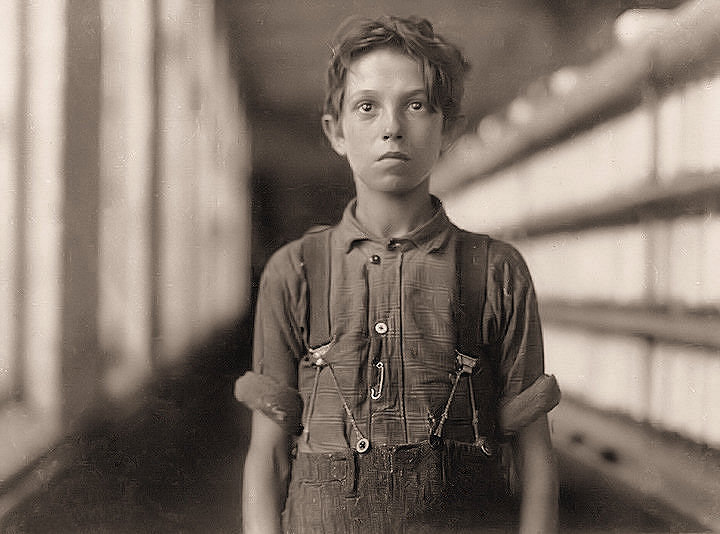
\includegraphics[width=3cm]{hine02}\par
  \raggedright
  \textit{Cover image: }
    The cover image shows Jo Bodeon, a back-roper in the mule room at 
    Chace Cotton Mill. Burlington, Vermont. This and other similar images 
    in this book were taken by Lewis W. Hine, in the period between 
    1908-1912. These images as well as social campaigns by many including 
    Hine, helped to formulate America's anti-child labour laws.
  \end{minipage}\par
  \vspace*{\baselineskip}
  \begin{minipage}[b]{0.9\textwidth}
  \RaggedRight
  \setlength{\parskip}{0.5\baselineskip}
  Copyright \copyright 2012  Dr Yiannis Lazarides\par
  Permission is granted to copy, distribute and\slash or modify this document 
  under the terms of the GNU Free Documentation License, version 1.2, with no 
  invariant sections, no front-cover texts, and no back-cover texts.\par
  A copy of the license is included in the appendix.\par
  This document is distributed in the hope that it will be useful, but without 
  any warranty; without even the implied warranty of merchantability or 
  fitness for a particular purpose.
  \end{minipage}
  \vspace*{2\baselineskip}
  \clearpage
}
%    \end{macrocode}
% \end{macro}
%
% \chapter{Table of Contents}
%
%	Most of the macros here re-write the LaTeX macros in a way that 
%	we can add appropriate hooks for styling. In writing this section
%	we had inspiration and used liberally code from Peter Wilson's 
%	\pkg{tocloft}. We have also borrowed the figure below as a
%   guideline.

%
% \newcommand{\maxx}{120}       ^^A picture width
% \newcommand{\maxxm}{118}      ^^A \maxx - 2\
% \newcommand{\maxy}{55}        ^^A picture height
% \newcommand{\maxym}{53}       ^^A \maxy - 2
% \newcommand{\findent}{20}     ^^A indent
% \newcommand{\findentp}{22}    ^^A \findent + 2
% \newcommand{\fnumwidth}{10}   ^^A numwidth
% \newcommand{\ftocrmarg}{30}   ^^A \@tocrmarg
% \newcommand{\fpnumwidth}{20}  ^^A \@pnumwidth
% \newcommand{\fipn}{30}        ^^A \findent + \fnumwidth
% \newcommand{\frmarg}{90}      ^^A \maxx - \ftocrmarg
% \newcommand{\frnum}{100}      ^^A \maxx - \fpnumwidth
% \newcommand{\fyi}{10}         ^^A 1st y height
% \newcommand{\fyim}{8}         ^^A \fyi - 2
% \newcommand{\fyii}{20}        ^^A 2nd y height
% \newcommand{\fyiii}{25}       ^^A 3rd y height
% \newcommand{\fyiv}{30}        ^^A 4th y height
% \newcommand{\fyv}{40}         ^^A 5th y height
% \newcommand{\fyvp}{42}        ^^A \fyv + 2
% \newcommand{\flin}{4}         ^^A length of leader lines
% \newcommand{\frmargm}{89}     ^^A \frmarg (90) - a little bit
% 
% \providecommand{\bs}{\textbackslash}
% \begin{figure}
% \centering
% \setlength{\unitlength}{1mm}
% \begin{picture}(\maxx,\maxy)
%     ^^A side lines and linewidth
%   \put(0,0){\line(0,1){\maxy}}
%   \put(\maxx,0){\line(0,1){\maxy}}
%   \put(0,\maxy){\vector(1,0){\maxx}}
%   \put(2,\maxym){\makebox(0,0)[tl]{\texttt{\bs linewidth}}}
%     ^^A \@pnumwidth
%   \put(\maxx,\fyi){\vector(-1,0){\fpnumwidth}}
%   \put(\maxxm,\fyim){\makebox(0,0)[tr]{\texttt{\bs @pnumwidth}}}
%   \put(\frnum,\fyi){\line(0,1){\flin}}
%     ^^A \@tocrmarg
%   \put(\maxx,\fyv){\vector(-1,0){\ftocrmarg}}
%   \put(\maxxm,\fyvp){\makebox(0,0)[br]{\texttt{\bs @tocrmarg}}}
%   \put(\frmarg,\fyv){\line(0,-1){\flin}}
%     ^^A indent
%   \put(0,\fyv){\vector(1,0){\findent}}
%   \put(2,\fyvp){\makebox(0,0)[bl]{\textit{indent}}}
%   \put(\findent,\fyv){\line(0,-1){\flin}}
%     ^^A numwidth
%   \put(\findent,\fyv){\vector(1,0){\fnumwidth}}
%   \put(\findentp,\fyvp){\makebox(0,0)[bl]{\textit{numwidth}}}
%   \put(\fipn,\fyv){\line(0,-1){\flin}}
%     ^^A last title line
%   \put(\maxx,\fyii){\makebox(0,0)[br]{487}}
%   \put(\fipn,\fyii){title end}
%     ^^A second title line
%   \put(\fipn,\fyiii){continue\ldots}
%   \put(\frmarg,\fyiii){\makebox(0,0)[br]{\ldots title}}
%     ^^A first title line
%   \put(\findent,\fyiv){\textbf{3.5}}
%   \put(\fipn,\fyiv){Heading\ldots}
%   \put(\frmarg,\fyiv){\makebox(0,0)[br]{\ldots title}}
%     ^^A dotted leader
%   \multiput(\frmargm,\fyii)(-\flin,0){12}{.}
%   \multiput(\frmarg,\fyi)(-\flin,0){2}{\line(0,1){\flin}}
%   \put(\frmarg,\fyi){\vector(-1,0){\flin}}
%   \put(\frmarg,\fyi){\vector(1,0){0}}
%   \put(\frmarg,\fyim){\makebox(0,0)[tr]{\texttt{\bs @dotsep}}}
% 
% \end{picture}
% \setlength{\unitlength}{1pt}
% \caption{Layout of a ToC (LoF, LoT) entry} \label{fig:ltoc}
% \end{figure}
%
% \begin{macro}{\quit@cx}
% \begin{macro}{\if@haschapter@cx}
% We will be using either chapter or section type headings for the ToC, etc.,
% so we need to know which of these the document class supports.
%    \begin{macrocode}
\newcommand{\quit@cx}{}
\newif\if@haschapter@cx
%    \end{macrocode}
% \end{macro}
% \end{macro}
% \begin{macro}{\if@koma@cx}
% The \pkg{koma} classes have different defaults than the standard classes,
% so we need to know if a \pkg{koma} class has been loaded.
%    \begin{macrocode}
\newif\if@koma@cx  \@koma@cxfalse
\@ifclassloaded{scrartcl}{\@koma@cxtrue}{}
\@ifclassloaded{scrreprt}{\@koma@cxtrue}{}
\@ifclassloaded{scrbook}{\@koma@cxtrue}{}
%    \end{macrocode}
% \end{macro}
%
% \begin{macro}{\if@memoir@cx}
%    \begin{macrocode}
\newif\if@memoir@cx  \@memoir@cxfalse
\@ifclassloaded{memoir}{\@memoir@cxtrue}{}
%    \end{macrocode}
% \end{macro}
%
% Issue a warning if there are no recognised sectional divisions 
% and then skip the rest of the package code.
%    \begin{macrocode}
\@ifundefined{chapter}{%
  \@haschapter@cxfalse
  \@ifundefined{section}{%
    \PackageWarning{phd}%
      {I don't recognize any sectional divisions so I'll do nothing}
    \renewcommand{\quit@cx}{\endinput}
    }{\PackageInfo{tocloft}{The document has section divisions}}
  }{\@haschapter@cxtrue
    \PackageInfo{phd}{The document has chapter divisions}}
%    \end{macrocode}
% bailing out or continue.
%    \begin{macrocode}
\quit@cx
%    \end{macrocode}
%
% \begin{macro}{\settocpagestyle}
% \begin{macro}{\tocpagestyle@cx}
%	We define a user macro and to be used in keys
%   a pagestyle for the first page of the ToC.
%   The default is the |plain| pagestyle. CHECK THIS.
%    \begin{macrocode}
\newcommand{\settocpagestyle}[1]{%
  \def\tocpagestyle@cx{\thispagestyle{#1}}}
  \thispagestyle{plain}
%    \end{macrocode}
% \end{macro}
% \end{macro}
%
% \begin{macro}{\tocparskip@cx}
% The |\parskip| local to the ToC, etc., is set to the length |\tocparskip@cx|.
%
%    \begin{macrocode}
\newlength{\tocparskip@cx}
\setlength{\tocparskip@cx}{0pt}
%    \end{macrocode}
% \end{macro}
%
% 
% \begin{macro}{\tableofcontents}
% This is a parameterised version of the default |\tableofcontents| command.
% Each class has its own definition, but we have to cater for all classes
% in one definition, hence some of the checks. The definition is
% modified after all packages have been loaded.
%	Consider more checks here
%
%    \begin{macrocode}
\def\tocstart@cx{}
\def\tocfinish@cx{}
   \renewcommand{\tableofcontents}{%
    \tocstart@cx
%    \end{macrocode}
% Ensure that any previous paragraph has been finished. Within a group set
% the local paragraphing style and typeset the title.
%    \begin{macrocode}
    \par
    \begingroup
      \parindent\z@ \parskip\tocparskip@cx
      \maketoctitle@cx
%    \end{macrocode}
%
% Finally, read the \file{.toc} file and finish up.
%    \begin{macrocode}
      \@starttoc{toc}%
    \endgroup
    \tocfinish@cx
}
%    \end{macrocode}
% \end{macro}
%
%    \begin{macrocode}
\cxset{toc name/.code = \def\contentsname{#1},
       toc name before/.store in = \contentsnamebefore@cx,
       toc name after/.store in = \contentsnameafter@cx,
       toc name font-size/.store in = \contentsnamefontsize@cx,
       toc name font-weight/.store in = \contentsnamefontweight@cx,
       toc name font-family/.store in = \contentsnamefontfamily@cx,
       toc name font-shape/.store in = \contentsnamefontshape@cx,
       toc name color/.store in = \tocnamecolor@cx,
       toc name afterskip/.store in=\tocnameafterskip@cx
}



\cxset{toc name= CONTENTS,
       toc name before = ,
       toc name after =, 
       toc name color = teal,
       toc name font-weight=bold,
       toc name font-family=sffamily,
       toc name font-shape=upshape,
       toc name font-size=LARGE,
       toc name afterskip=10pt, %set as 40pt in LaTeX
       toc name after=\par,
}

\newcommand{\maketoctitle@cx}{%
  \addpenalty\@secpenalty
  \if@haschapter@cx
    \vspace*{10pt}
  \else
    \vspace{10pt}
  \fi
  %\@cftpagestyle
  {\interlinepenalty\@M
  {\contentsnamebefore@cx
     \setfont@cx{\contentsnamefontweight@cx}%
    {\contentsnamefontfamily@cx}{\contentsnamefontsize@cx}%
    {\contentsnamefontshape@cx}%
     \color{\tocnamecolor@cx}
      \center\contentsname\endcenter}{\contentsnameafter@cx}
    
  \par\nobreak
  \vskip\tocnameafterskip@cx\relax
  \@afterheading}
}
%    \end{macrocode}
%
% \begin{macro}{\cftsetpnumwidth}
% \begin{macro}{\cftsetrmarg}
%  Users commands for setting |\@pnumwidth| and |\@tocrmarg|.
%    \begin{macrocode}
\newcommand{\setpnumwidth@cx}[1]{\renewcommand{\@pnumwidth}{#1}}
\newcommand{\settocmarg@cx}[1]{\renewcommand{\@tocrmarg}{#1}}
\setpnumwidth@cx{25pt}
\settocmarg@cx{20pt}
%    \end{macrocode}
% \end{macro}
% \end{macro}
%
% \section{Styling the dot leaders}
%  	Here we will allow the user to either have dotfills andto be
%	able to specify the type and spacing of the dots.
%	We will alsoprovide a key to disable dotfills.
%
% \begin{macro}{\dot@cx}
% \begin{macro}{\dotfill@cx}
%   In the default ToC, a dotted line can be used to provide a leader between
%   a title and the page number. As Peter Wilson wrote and I found at my
%   distress the definition of the leader is buried
%   in the |\@dottedtocline| command. The |\dotfill@cx{|\meta{sep}|}|
%   command provides a parameterised version of the leader code, where
%   \meta{sep} is the seperation between the dots in mu units.
%   The symbol used for the `dots' in the leader is given by the value
%   of |\dot@cx|. 
% 
%    \begin{macrocode}
\newcommand{\dot@cx}{.}
\newcommand{\dotfill@cx}[1]{%
  \leaders\hbox{$\m@th\mkern #1 mu\hbox{\dot@cx}\mkern #1 mu$}\hfill}
%    \end{macrocode}
% \end{macro}
% \end{macro}
%
%    \begin{macrocode}
\def\nodotfill@cx{}
\cxset{toc dotfill/.is choice,
       toc dotfill/none/.code = \nodotfill@cx,
       toc dotfill symbol/.code= \renewcommand{\dot@cx}{#1},
       toc dotfill sep/.store in=\dotfillsep@cx,
}
\cxset{toc dotfill symbol=.,
       toc dotfill sep=4.5}
%    \end{macrocode}
%
% \begin{macro}{\cftparfillskip}
% The |\l@kind| commands modify (locally) the value of |\parfillskip|.
% |\cftparfillskip| is a copy of the default \textit{\TeX book}
% |\parfillskip| definition.
%    \begin{macrocode}
\newcommand{\cftparfillskip}{\parfillskip=0pt plus1fil}
%    \end{macrocode}
% \end{macro}
%
% \begin{macro}{\numberline}
% The purpose of the |\numberline{|\meta{secnum}|}| command is to typeset
% \meta{secnum} left justified in a box of width |\@tempdima|. I redefine
% it to add three additional parameters, namely |\@cftbsnum|, 
% |\@cftasnum| and |\@cftasnumb| 
% (see \file{ltsect.dtx} for the original
% definition).
%    \begin{macrocode}
\renewcommand{\numberline}[1]{% 
  \hb@xt@\@tempdima{\@cftbsnum #1\@cftasnum\hfil}\@cftasnumb}
%    \end{macrocode}
% \end{macro}
%
% \begin{macro}{\@cftbsnum}
% \begin{macro}{\@cftasnum}
% \begin{macro}{\@cftasnumb}
% \changes{v0.2b}{1999/03/07}{Added empty definitions for @cftasnum and @cftasnumb commands}
% \changes{v1.1}{2000/02/11}{Added empty definition of \cs{@cftbsnum}}
% Originally these were not defined but were |\let| to appropriate commands
% in the |\l@...| commands, but they
% have to be defined in case something unexpected calls |\numberline|,
% for example through use of the \Lpack{float} package.\footnote{This bug
% was discovered by Andrew Thurber when using the \Lpack{tocloft} and
% \Lpack{algorithm} packages together.}
%
%    \begin{macrocode}
\newcommand{\@cftbsnum}{}
\newcommand{\@cftasnum}{}
\newcommand{\@cftasnumb}{}
%    \end{macrocode}
% \end{macro}
% \end{macro}
% \end{macro}

% \begin{macro}{\beforetocchapterskip@cx}
% \begin{macro}{\cftchapindent}
% \begin{macro}{\cftchapnumwidth}
% \begin{macro}{\cftchapfont}
% \begin{macro}{\cftchappresnum}
% \begin{macro}{\cftchapaftersnum}
% \begin{macro}{\cftchapaftersnumb}
% \begin{macro}{\cftchapleader}
% \begin{macro}{\cftchapdotsep}
% \begin{macro}{\cftchappagefont}
% \begin{macro}{\cftchapafterpnum}
% \begin{macro}{\cftchapfillnum}
%  These are the user commands to control the typesetting of Chapter entries.
%  They are initialised to give the standard appearance.
%    \begin{macrocode}

\if@haschapter@cx
  \newlength{\beforetocchapterskip@cx}
    \setlength{\beforetocchapterskip@cx}{1.0em \@plus\p@}
  \newlength{\cftchapindent}
    \setlength{\cftchapindent}{0em}
  \newlength{\cftchapnumwidth}
    \setlength{\cftchapnumwidth}{1.5em}
  \newcommand{\cftchapfont}{\bfseries}
  \newcommand{\cftchappresnum}{}
  \newcommand{\cftchapaftersnum}{}
  \newcommand{\cftchapaftersnumb}{}
  \newcommand{\cftchapleader}{\bfseries\dotfill@cx{\cftchapdotsep}}
%    \end{macrocode}

%	The following code determines the spacing of he dots.
%    \begin{macrocode}
  \newcommand{\cftchapdotsep}{\chapterdotsep@cx} 
  \newcommand{\cftchappagefont}{[\sffamily\bfseries\color{red}}
  \newcommand{\cftchapafterpnum}{]}
  \newcommand{\cftchapfillnum}[1]{%
    {\cftchapleader}\nobreak
    \hb@xt@\@pnumwidth{\hfil\cftchappagefont #1}\cftchapafterpnum\par}
%    \end{macrocode}
% \Lpack{koma} classes have different chapter settings.
% \changes{v2.3}{2002/06/15}{koma has different chapter settings}
%%    \begin{macrocode}
%  \if@cftkoma
%    \renewcommand{\cftchapfont}{\sectfont}
%  \fi
\fi

%    \end{macrocode}
% \end{macro}
% \end{macro}
% \end{macro}
% \end{macro}
% \end{macro}
% \end{macro}
% \end{macro}
% \end{macro}
% \end{macro}
% \end{macro}
% \end{macro}
% \end{macro}
% \begin{macro}{\l@chapter}
%  \cs{l@chapter}\marg{title}\marg{page} typesets the ToC entry for
% a |chapter| heading. It is a parameterised copy of the default |\l@chapter|
% (see \file{classes.dtx} for the original definition). This only applies
% to chaptered documents.
%    \begin{macrocode}

\renewcommand{\numberline}[1]{% 
  \hb@xt@\@tempdima{[#1]\hfil}}


\cxset{toc chapter beforeskip/.store in=\beforetocchapterskip@cx,
       toc chapter indent/.store in = \tocchapterindent@cx,
       toc chapter dotsep/.store in = \chapterdotsep@cx,
       toc chapter no dots/.code=\def\chapterdotsep@cx{10000},
       toc chapter numberwidth/.store in = \tocchapternumberwidth@cx,
       toc chapter font/.store in=\tocchapterfont@cx}


\cxset{toc chapter beforeskip =40pt,
       toc chapter indent= 0pt,
       toc chapter dotsep=4.5,
       toc chapter no dots,
       toc chapter numberwidth=15pt,
       toc chapter font= \bfseries\sffamily\large}

\if@haschapter@cx
\renewcommand*{\l@chapter}[2]{%
  \ifnum \c@tocdepth >\m@ne
    \addpenalty{-\@highpenalty}%
    \vskip \beforetocchapterskip@cx\relax
    {\leftskip\tocchapterindent@cx\relax
     \rightskip \@tocrmarg
     \parfillskip -\rightskip
     \parindent \tocchapterindent@cx\relax\@afterindenttrue
     \interlinepenalty\@M
     \leavevmode
     \@tempdima \tocchapternumberwidth@cx\relax
     \let\@cftbsnum \cftchappresnum
     \let\@cftasnum \cftchapaftersnum
     \let\@cftasnumb \cftchapaftersnumb
     \advance\leftskip \@tempdima \null\nobreak\hskip -\leftskip
     {\tocchapterfont@cx #1}\nobreak
     \cftchapfillnum{#2}}%
  \fi}%
\fi
%    \end{macrocode}
% \end{macro}
%

%
%\iffalse
%</package>
%\fi
% \appendix
% \cxset{
%  chapter name = Appendix,
%  section numbering prefix = \thechapter.}
%  
% \chapter{MWE and Testing Macros}
%
% As far as LaTeX is concerned, there is nothing special in styling an appendix. It is either a chapter or a section with a different name. This name in order to allow internationalization is called \lstinline{\appendixname}.
%\bigskip
%
%\begin{tcolorbox}[width=\linewidth]
%\begin{lstlisting}
%\newcommand\appendix{\par
%  \setcounter{chapter}{0}%
%  \setcounter{section}{0}%
%  \gdef\@chapapp{\appendixname}(*@\footnote{The actual literal used for   \textbackslash{appendixname} is defined later on, so that you can customize the language}\label{appendixname}@*)
%  \gdef\thechapter{\@Alph\c@chapter}
%}
%\end{lstlisting}
%\end{tcolorbox}
%\medskip
%
%The code above is only a simplified version of the command. One might need to add more formatting information such as resetting equation numbers, tables and figures and any special floating environments that have their own numbering.
%
%\begin{tcolorbox}[width=\linewidth]
%\begin{lstlisting}
%\renewcommand\appendix{\par
%                \stepcounter{chapter}
%                \setcounter{chapter}{0}
%                \stepcounter{section}
%                \setcounter{section}{0}
%                \setcounter{equation}{0}
%                \setcounter{figure}{0}
%                \setcounter{table}{0}
%                \setcounter{footnote}{0}
%  \def\@chapapp{\appendixname}%
%  \renewcommand\thechapter{\@Alph\c@chapter}}
%\end{lstlisting}
%\end{tcolorbox}
%
% \section{Test macros}
% We provide a series of MWE for testing purposes.
% \subsection{Letter MWE}
% \iffalse
%<*MWE-01>
% \fi
% \subsection{MWE-01, using \texttt{multicol} and \texttt{multitoc}}
%    \begin{macrocode}
%^^A This is an example using the default |lstlisting|
%^^A environment.
\documentclass{article}
\usepackage{phd}
\begin{document}
  \begin{lstlisting}
    \def\test{This is a test.}  
  \end{lstlisting}
  \begin{teX}
    \def\test{This is a test.} 
  \end{teX}
  \begin{teXX}
    \def\test{This is a test.} 
  \end{teXX}
  
  \startnumberat{25}
  \begin{teX}
    \def\test{This is a test.} 
  \end{teX}
  
  \startnumberat{35}
  \begin{teX}
    % coloring comments is done in orange
    \def\test{This is a test.} 
  \end{teX}
\end{document}
%    \end{macrocode}
% \iffalse  
%</MWE-01>
% \fi
% \iffalse
%<*MWE-02>
% \fi
% \subsection{Listings MWE-02}
%    \begin{macrocode}
%% Example using |multitoc|
\documentclass{article}
\usepackage{phd}
\renewcommand{\multicolumntoc}{2}
\title{Typesetting the Table of Contents in Multiple Columns}
\author{Dr Y. Lazarides}
\begin{document}
\maketitle
\tableofcontents
\section{First section}
\begin{multicols}{3}
\lipsum[1-2]
\end{multicols}
\subsection{First subsection}
\subsection{Second subsection}
\subsection{Third subsection}
\subsection{Last subsection}
\section{Second section}
\subsection{First subsection}
\subsection{Second subsection}
\subsection{Third subsection}
\subsection{Last subsection}
\section{Last section}
\subsection{First subsection}
\subsection{Second subsection}
\subsection{Third subsection}
\subsection{Last subsection}
\end{document}
%    \end{macrocode}
% \iffalse  
%</MWE-02>
% \fi
% 
% \subsection{Listings MWE-03}
% 
% \iffalse
%<*MWE-03>
% \fi
%    \begin{macrocode}
%% example for using encoded commands such as guillemets. (If you need
%% shorthands you need to load babel.
%%
\documentclass{article}
\usepackage{phd}
\newcommand{\encone}[1]{{\fontencoding{T1}\selectfont#1}}
\begin{document}
\def\Kt#1{{\encone{#1}} &{\small\ttfamily\string#1}}

\noindent\begin{tabular}{@{}*8l@{}}
\toprule
\Kt\guillemotleft  & \Kt\guilsinglleft & \Kt\quotedblbase & \Kt\textquotedbl \\
\Kt\guillemotright & \Kt\guilsinglright & \Kt\quotesinglbase \\
\bottomrule
\end{tabular}
\medskip

\lipsum[1]
\end{document}
%    \end{macrocode}
% \iffalse  
%</MWE-03>
% \fi
% 
% \iffalse
%<*test-tufte>
% \fi
%    \begin{macrocode}
\documentclass[justified]{tufte-book}
\usepackage{phd}
\begin{document}
\lipsum[1]
\sidenote{\RaggedRight \protect\lipsum[5]}
\centering
\begin{minipage}{5cm}
\RaggedRight

\lipsum[1]
\end{minipage}
\end{document}
%    \end{macrocode}
% \iffalse  
%</test-tufte>
% \fi
%
% \iffalse
%<*test-memoir>
% \fi
%    \begin{macrocode}
% clashes with options
\documentclass{memoir}
\usepackage{phd}
\begin{document}
\lipsum[1]
\end{document}
%    \end{macrocode}
% \iffalse  
%</test-memoir>
% \fi
%
%\iffalse
%<*test-scrartcl>
% \fi
%    \begin{macrocode}
% clashes with options
\documentclass{scrartcl}
\usepackage{phd}
\begin{document}
\lipsum[1]

\[ A = \upalpha r^2/4\]

% check for complaints
$$ A = a + b $$
\end{document}
%    \end{macrocode}
% \iffalse  
%</test-scrartcl>
% \fi
% 
%\iffalse
%<*test-hyphenation>
% \fi
%    \begin{macrocode}
\documentclass{scrartcl}
\usepackage{phd}
\begin{document}
%% Tests if hyphenation routines have been
%% found.
\hsize2cm
\noindent Florida appendix asynchronous
\end{document}
%    \end{macrocode}
% \iffalse  
%</test-hyphenation>
% \fi
%
%\iffalse
%<*test-algorithms>
% \fi
%    \begin{macrocode}
% clashes with options
\documentclass{article}
\usepackage{phd}
\begin{document}
\begin{algorithm}[H]
\SetAlgoLined
\KwData{this text}
\KwResult{how to write algorithm with \LaTeX2e }
initialization\;
\While{not at end of this document}{
read current\;
\eIf{understand}{
go to next section\;
current section becomes this one\;
}{
go back to the beginning of current section\;
}
}
\caption{How to write algorithms}
\end{algorithm}
\IncMargin{1em}
\begin{algorithm}
\SetKwData{Left}{left}\SetKwData{This}{this}\SetKwData{Up}{up}
\SetKwFunction{Union}{Union}\SetKwFunction{FindCompress}{FindCompress}
\SetKwInOut{Input}{input}\SetKwInOut{Output}{output}
\Input{A bitmap $Im$ of size $w\times l$}
\Output{A partition of the bitmap}
\BlankLine
\emph{special treatment of the first line}\;
\For{$i\leftarrow 2$ \KwTo $l$}{
\emph{special treatment of the first element of line $i$}\;
\For{$j\leftarrow 2$ \KwTo $w$}{\label{forins}
\Left$\leftarrow$ \FindCompress{$Im[i,j-1]$}\;
\Up$\leftarrow$ \FindCompress{$Im[i-1,]$}\;
\This$\leftarrow$ \FindCompress{$Im[i,j]$}\;
\If(\tcp*[h]{O(\Left,\This)==1}){\Left compatible with \This}{\label{lt}
\lIf{\Left $<$ \This}{\Union{\Left,\This}}\;
\lElse{\Union{\This,\Left}\;}
}
\If(\tcp*[f]{O(\Up,\This)==1}){\Up compatible with \This}{\label{ut}
\lIf{\Up $<$ \This}{\Union{\Up,\This}}\;
\tcp{\This is put under \Up to keep tree as flat as possible}\label{cmt}
\lElse{\Union{\This,\Up}}\tcp*[r]{\This linked to \Up}\label{lelse}
}
}
\lForEach{element $e$ of the line $i$}{\FindCompress{p}}
}
\caption{disjoint decomposition}\label{algo_disjdecomp}
\end{algorithm}\DecMargin{1em}
\end{document}
%    \end{macrocode}
% \iffalse  
%</test-algorithms>
% \fi
%
%<*test-spacing>
% Uses the package setspace to set the spacing of the
% document.
%    \begin{macrocode}
\documentclass{article}
\usepackage{setspace}
\usepackage{lipsum}
\onehalfspacing
\begin{document}
\title{merry setspace christmas test}
\author{who cares?}
\date{2011-12-19}
\maketitle

\section{dummy}
\lipsum[1]
\subsection{first offspring}
\lipsum[2]
\begin{tabular}{llr}
  a & silly & story about latex \\
  silly & a & story
\end{tabular}
\end{document}
%    \end{macrocode}
%</test-spacing>
%
% \iffalse
%<*settings>
% \fi
%% Some settings
%    \begin{macrocode}
\cxset{nag keys = {l2tabu,%
                   orthodox}}
\cxset{onlyamsmath keys = {all}}
%    \end{macrocode}
% \iffalse
%</settings>
% \fi
%
% \PrintIndex
%
% \Finale

% \newpage
%
% \section{List of Packages and Usage Statistics}
%
% Table~\ref{tbl:listofpaks} provides a list of the packages loaded as default by |phd|.
% The column describing usage statistics
% is from \url{http://arxmliv.kwarc.info/package_usage.php}. It is by no means an
% indication of overall popularity, but I have used these statistics as an
% guide in selecting what packages to include here in order to at least cover
% the scientific side well.
%
% 
\setcounter{step}{0}
\begingroup
\centering
\begin{longtable}{llp{3.5cm}p{3.5cm}}
\toprule
Ser.  &Usage &Remarks\\
\midrule
\inc &fixltx2e & patches to LaTeX2e&\\
\inc &nag      & nag provides routines to warn
                 user against using outdated
                 packages and commands.           &\\
\inc &nag      & microtype&\\
\inc &onlyamsmath &This package inhibits 
					the usage of 
                plain TEX and 
                on demand of standard
					LATEX math environments. 
					This is useful for class writers 
					who want to force
					their clients to use the environments 
					provided by the amsmath package. &\\
\midrule
\inc &graphicx  &  & \\
\inc &wrapfig   &  & \\
\inc &rotating  &  & \\
\inc &subfig    &  & \\
\inc &xcolor    &  & If loaded by class we skip \\
\midrule
\inc &booktabs  &  & \\
\inc &tabularx  &  &\\
\inc &dcolumn   &  &\\
\inc &longtable &  &\\
\inc &colortabl &  &\\
\inc &multirow  &  &\\
\inc &landscape & &\\
\inc &threeparttable & &\\
\midrule
\inc &array     & &\\
\inc &amsfonts  & &\\
\inc &amsmath   & & (66226)\\
\inc &amssymb   & & (74838)\\
\inc &amsthm    & & (15606)\\
\inc &mathtools & &\\
\inc &stmaryd   & &\\
\inc &xpfeil    & &\\
\inc &extpfeil  & &\\
\inc &euscript  &For calligraphic fonts &\\
\inc &bm        &                       &\\
\inc &bbm       &                       &(2200)\\
\inc &upgreek   &                       & \\
\midrule
\multicolumn{4}{c}{Symbols}\\
\midrule
\inc &latexsym  & &\\
\inc &wasymsym  & &\\
\inc &textcomp  & &\\
\inc &pifont    & &\\
\inc &marvosym  & &\\
\inc &manfnt    & &\\
\inc &bbding    & &\\
\inc &ifsym     & &\\
\inc &eurosym   & &\\
\midrule
\inc &epigraph  & &\\
\inc &siunitx   & &\\
\inc &filecontents & &\\
\midrule
\inc & changepage         & &\\
\inc & keyval             & &\\
\inc & ifmtarg            & &\\
\inc & fp                & &\\
\inc & ifthen             & &\\
\inc & xstring            & &\\
\inc & etoolbox           & &\\
\inc & algorithms         & &\\
\inc & algorithmicx       & &\\
\inc & algorithm2e        & &\\
\midrule
\inc & multicol           & &\\
\inc & multitoc           & &\\
\inc & ragged2e           & &\\
\inc & soul               & &\\
\inc & xspace             & &\\
\inc & ulem               & &\\
\inc & alltt              & &(259)\\
\bottomrule
\inc & idxlayout          & &\\
\bottomrule
\inc & tcolorbox          & &\\
\inc & listings           & &\\
\midrule
\multicolumn{4}{c}{Miscellaneous} \\
\midrule
\inc & fourier/fourier-orns & ornaments/math  &\\
\inc & cclicenses         & &\\
\inc & dirtree            &directory trees &\\
\midrule
\multicolumn{4}{c}{Archaic} \\
\midrule
\inc  &linearA & &\\
\inc  &linearB & &\\
\inc  &cypriot & &\\
\inc  &sarabian & &\\
\bottomrule
\end{longtable}
^^A\captionof{table}{List of packages loaded by the phd package.}
\endgroup

% \label{tbl:listofpaks}
\endinput

http://tex.stackexchange.com/questions/45651/how-do-i-determine-in-which-order-packages-have-been-loaded
% ^^A\addtocontents{toc}{\protect\end{multicols}}
%\begin{thebibliography}{1}
%\raggedright
%
%\bibitem{companion}
%Frank Mittelbach et al.:
%\textit{The LaTeX Companion}.\\
%2nd edition. Addison Wesley, 2004.
%
%
%\bibitem{fntguide}
%\LaTeX3 Project Team (Ed.):
%\textit{LaTeX2e font selection.}\\
%CTAN: \path{macros/latex/doc/fntguide.pdf}\\
%(Part of the \LaTeX{} online documentation)
%
%\bibitem{marvosym}
%Thomas Henlich,Mojca Miklavec:
%\textit{The MarVoSym Font Package}
%
% ^^A\end{thebibliography}
%
For custom section
\makeatletter
\renewcommand\thesubsection{\thesection.\two@digits{\value{subsection}}}
\renewcommand\thesubsubsection{\thesubsection.\two@digits{\value{subsubsection}}}
\makeatother

TODO 

Check why maketitle does not work

%^^A 

\makeatletter
\cxset{toc image=\@empty}

\@specialtrue
\setdefaults 
\renewcommand\stewart[2][]{%
\fancypagestyle{fancy}{%
\lhead{}\rhead{}
\chead{}
\cfoot{}
\lfoot{}
\rfoot{\thepage}
\def\footrule#1{{\color{blue}%
  \hrule width\paperwidth}\vskip3pt
}

\renewcommand{\headrulewidth}{0pt}
\renewcommand{\footrulewidth}{0.4pt}}

\clearpage

\begin{tikzpicture}[remember picture,overlay]
% Main shading block
\node [xshift=5cm,yshift=-\paperheight] at (current page.north west)
[text width=0.98\textwidth,text height=\paperheight, fill=thecream!30,rounded corners,above right]
{};
\node [xshift=6.5cm,yshift=-1.5cm-\soffsety] at (current page.north west)
[text width=0.9\textwidth,below right]{\sffamily \bfseries \huge #2};

\node [xshift=3cm,yshift=-1.5cm] at (current page.north west)
[text width=3cm,align=center,minimum height=2.5cm, fill=blue,below right]
{\[\text{\HHUGE\bfseries\sffamily\color{white}\thechapter}\]
\par\vspace*{3pt}
};

\node [xshift=-0.2cm,yshift=-21.5cm] at (current page.north west)
[text width=3cm,above right]%
{\includegraphics[width=1.0\paperwidth]{./chapters/\image@cx}};
% second box left
\node [xshift=3cm,yshift=-19.5cm] at (current page.north west)
[text width=9cm,minimum height=2.5cm,inner sep=0.5em, fill=blue,below right]
{\color{white}
  \bfseries\sffamily \texti@cx
};
% Last block
\node [xshift=6.5cm,yshift=-26cm] at (current page.north west)
[text width=12cm,above right]
{\textii@cx
};
\end{tikzpicture}
\par
\clearpage
}





\cxset{steward,
  numbering=arabic,
  custom=stewart,
  offsety=0cm,
  image=hine03,
  texti={When Lamport designed the original \LaTeX\ sectioning commands he did not provide a fully comprehensive interface for modifying their design. With current tools available improvements are much easier to program and this chapter provides the details.},
  textii={\precis{In this chapter we discuss a method that allows the production of fancy chapter headings and formatting, based on a set of key values. Central  to this process is the separation of content from presentation.
We also discuss the basic formatting tools that are available and how one can modify them to mould new book designs.}
 }
}


\chapter{Designing Chapters}

\section{Introduction}

For too long, the act of printing something in and of itself has been placed on too high a pedestal. The true value of an object lies in what it says, not its mere existence. And in the case of a book, that value is intrinsically connected to content. The aim of this package is to try and provide a bridge between separating content from presentation.

A new chapter must make a good impression and must give an immediate signal that something different is going to be written. Traditionally chapter openings in LaTeX are an unimpressive and dry event. Our aim is to brighten it up a bit, while keeping true separation of content from presentation.



\section{Package Usage}

To use the package include it just like any other package:

\begin{tcolorbox}
\begin{lstlisting}
\documentclass{book}
\usepackage{chaptersx}
\cxset{style13}
\begin{document}
\chapter{Introduction}
\end{document}
\end{lstlisting}
\end{tcolorbox}

The command \cs{cxset} sets the default style for the example to the style defined as \marg{style13}. The package currently offers over 50 styles and numerous keys to manipulate them further.



\section{Chapter opening page}

The standard LaTeX classes offer only two options to either open a chapter on an odd page or at any page. This package offers five alternatives:

\keyval{chapter opening}{\marg{any, left, right, anywhere, ifafter}}{The various keys enable any combination to be used.}

\begin{marglist}
\item [any] Opens a chapter at any page, either verso or recto.
\item [left] Opens a chapter on an even page
\item [right] Opens a chapter on a right page.
\item [anywhere] Opens a chapter at the point where the \cs{chapter} is typed.
\item [none] Alias for \marg{anywhere}.
\item [ifafter] Opens a chapter at the next page if the page has material that does not exceed a certain portion of \cs{textheight}.
\end{marglist}

To change a setting you just modify the value of the key \option{chapter opening} to one of the values described earlier.

\begin{tcolorbox}
\begin{lstlisting}
\cxset{chapter opening=anywhere}
\end{lstlisting}
\end{tcolorbox}

\@specialfalse
\cxset{chapter toc=false}
\begin{texexample}{title=Inline Chapter Example}{ex:anywhere}
\cxset{chapter opening=anywhere, chapter before=\bigskip, chapter font-family=\sffamily,title font-family=\sffamily}

\lipsum[2]
\chapter{Chapter Example}
\lipsum[3]
\chapter{Another Chapter Example}
\lipsum[4]
\end{texexample}



\addtocounter{chapter}{-1}

Examples for other types of chapter openings follow in the rest of the documentation.

\subsection{Blank pages before chapters}
In the standard LaTeX book class when the openany option is not given or in the report class when the openright is given, chapters start at odd-numbered pages. This can cause a blank page to be printed. Some book designers prefer this page to be completely empty, without any headers or footers. This cannot be done with \lstinline{\thispagestyle} as this command will have to be issued on the \textit{previous} page. However by a suitable redefinition of the
\lstinline{\clearpage} this can be done automatically.
\medskip

\begin{tcolorbox}
\begin{lstlisting}
\makeatletter
\def\cleardoublepage{\clearpage\if@twoside\ifodd\c@page\else
  \hbox{}
  \vspace*{\fill}
  \begin{center}
    This page left intentionally blank.
  \end{center}
  \vspace{\fill}
  \thispagestyle{empty}
  \newpage
  \if@twocolumn\hbox{}\newpage\fi\fi\fi}
\makeatother
\end{lstlisting}
\end{tcolorbox}
\medskip

This is achieved easily by setting the following options:
\bigskip

\begin{tcolorbox}
\lstinline{chapter blank page=empty}\par
\lstinline{chapter blank page text=Some text.}\par
\lstinline{chapter blank page=plain}\par
\end{tcolorbox}
\medskip



The last one refers to a \lstinline!\thispagestyle{plain}!.

\section{Keys for chapter head formatting}

A chapter heading can be considered of being constructed of several parts, the \textit{chapter number}, the chapter name typically \textit{chapter} and the \textit{title}. Predefined keys handle all the elements of formatting. Additional keys are defined to handle other elements such as inclusion of images or producing complicated examples with graphics constructed with TikZ or other similar packages.

\medskip

\keyval{chapter numbering font-size}{\oarg{sizing commands}}{}.
\keyval{chapter numbering font-family}{\oarg{sizing commands}}{}.

\subsection{Keys for numbering}
Chapter numbering follows that of the standard \LaTeX\ classes and is extended to cover some additional cases such as fully spelled out numbers.

\keyval{number numbering}{\oarg{alph,Alph,roman,Roman,none,WORDS,words}}{Style of numbering.}
\medskip

\parindent1.5em

Note that the package uses Heiko Oberdiek's package alphalph to allow for alphabetic numbering that extends beyond the normal 26 letters of the alphabet. Examples for numbering can be seen in \ref{ex:romannumbering}

\medskip




\begin{marglist}
\item [arabic] Despite that the Arabs call what the West calls Arabic numbers Indian numbers, we provide the value arabic to have normal numbers printed.
\item [alph] Lowercase alphabetic numbering.
\item [Alph] Uppercase alphabetic numbering.
\item [roman] Lowercase roman numbering.
\item [Roman] Uppercase roman numbering.
\item [words]
\item [WORDS]
\item [Words] Prints the number in words and capitalizes the first letter, for example the number 21 will be printed as `Twenty One'\footnote{Currently limited to the first hundred numbers}.
\item [none] This is equivalent to using the star version of the command. It does not print any number and does not increment the chapter counter.\footnote{I am ambivalent about this, perhaps it will be better to increment it, as it can give a more general approach.}
\end{marglist}

\cxset{chapter opening=anywhere, numbering=Roman}
\index{chapter design!numbering!roman}
\begin{texexample}{Setting up keys for numbering}{ex:romannumbering}
\cxset{numbering=Roman}
\chapter{Roman numbering}
\end{texexample}



\clearpage

\index{chapter design!numbering!words}
\begin{texexample}{title=Chapter number in words}{}
\cxset{numbering=WORDS}
\chapter{Literal numbering}
\end{texexample}



\cxset{numbering=arabic}
\subsection{Setting font information}
\subsection{Letter spacing}

Chapter letter spacing can be achieved using the soul package in a combination with the key spaceout.
\medskip



\keyval{chapter spaceout}{\marg{soul}}{Uses the soul package to space out the lettering of chapter, number or the chapter name.}\par\medskip



The following examples illustrate the usage.

\begin{texexample}{}{}
\cxset{numbering=Roman,
         chapter spaceout=none,
         title spaceout=soul,
         title font-size=\Large,
         title font-family=\rmfamily,
         title font-shape=\scshape}
\chapter{Letter Spacing}
\end{texexample}



\index{chapter design!labels!letter spacing}
\begin{texexample}{}{} 
\cxset{chapter spaceout=soul,numbering=arabic, title spaceout=soul}
\chapter{Chapter title}
\end{texexample}



\subsection{Styling the title}

Similarly to the number and chapter styling keys exist for styling the title. We summarize the available standard keys below:
\medskip

  \keyval{chapter title font-family}{\marg{family}}{Selects a predefined font family}
  \keyval{chapter title font-weight}{\marg{\cs{bfseries},\cs{normalseries}}}{Font weight.}
  \keyval{chapter title font-size}{\marg{\cs{large},\cs{Large},\cs{huge},\cs{Huge},\cs{HUGE},\cs{HHuge}}}{Font sizing command.}
  \keyval{chapter title font-color}{}{}
  \keyval{chapter title spaceout}{\marg{soul,none}}{}
  \keyval{title before}{}{}
 \keyval{title after}{}{}
  \keyval{title beforeskip}{}{}
  \keyval{title afterskip}{}{}


\begin{texexample}{letter spacing the chapter title block}{}
\cxset{style13, chapter spaceout=none,
       numbering=arabic}
\chapter{Chapter Title Styling}
\end{texexample}



The last example illustrated the use of a predefined style \oarg{style13} and overriding some of the parameters.


\cxset{chapter opening=right}
\section{Table of Contents}\index{table of contents!key settings}

Traditionally a chapter will be added to the Table of Contents if the \cs{chapter} command is issued. The starred version will not produce a number and will not add a contents line. Since we have adopted an approach where we use a key value interface we can dispense with the starred version of the command, by setting the \option{chapter toc} option to false. For example if we want to define a command for a ``Foreward'' or ``Epiloque'' without wishing them to be added to the table of contents we can use the following setting.\index{Foreward!definitions}\index{Epilogue!definitions}



\begin{texexample}{changing the chapter label name}{}
\cxset{chapter toc=false, name=, numbering=none,}
\chapter{Foreward}
\lorem
\end{texexample}

Note that the key \option{numbering=none} still has to be set.


Please note that when \textbf{numbering=none} the chapter number is not available anymore and yo may have to reset it if required again. Although this might be seen as rather cumbersome than simply using \cs{chapter*} the advantage is consistency in the user interface and the use of appropriate semantic definitions for all sectioning commands thus achieving a bit more separation of context from style.


\cxset{chapter toc=true}

\section{Defining styles}

Named styles can be defined using the standard \textsc{PGF} conventions. To define a style for the forward above we can use:

\begin{texexample}{}{}
\cxset{foreward/.style={chapter toc=false,numbering=none,
          name=,
          title font-size= Large,
          title font-family= sffamily,
          numbering=none}}
\cxset{foreward}
\chapter{Foreward.}
\lorem
\end{texexample}



\cxset{numbering=arabic}
\section{Creating semantic names for commands and environments}

To keep our search for semantic commands and true separation of contents it is prudent to define some macros for typesetting the  `foreward' section.

\begin{texexample}{defining a \textit{Foreward} macro.}{}
\begin{lstlisting}
\cxset{foreward/.style={chapter toc=false,
          name=,
          title font-size = Large,
          title font-family = sffamily,
          numbering=none}}
\newcommand\forewardname{foreward}
\expandafter\newenvironment\expandafter{\forewardname}{%
\cxset{foreward}\chapter{Foreward}}%
{}
\begin{foreward}
\lorem
\end{foreward}
\end{lstlisting}
\end{texexample}



Notice the use of a new command \cs{forewardname} to allow for internationlization using Babel or other methods. One is tempted to let the English name, but a better approach perhaps is to define both.



% \makeatletter\@specialfalse
\cxset{custom = stewart}
\cxset{steward,
  numbering=arabic,
  custom=stewart,
  offsety=0cm,
  image={./images/hine03.jpg},
  texti={When Lamport designed the original \LaTeX\ sectioning commands he did not provide a fully comprehensive interface for modifying their design. With current tools available improvements are much easier to program and this chapter provides the details.},
  textii={\precis{In this chapter we discuss a method that allows the production of fancy chapter headings and formatting, based on a set of key values. Central  to this process is the separation of content from presentation.
We also discuss the basic formatting tools that are available and how one can modify them to mould new book designs.}
 }
}


\cxset{epigraph rule color=teal,epigraph width=0.37\textwidth\relax}

\chapter{Epigraphs}\index{epigraphs}
\label{c:epigraphs}

\epigraph{Please give examples of good use of epigraphs in fiction.

I mean them quoted dealies they sometimes put at the start of chapters.

What counts as ``good use" is whatever you think counts. Part of my goal is to understand what people like about these things.
.}{\href{http://ask.metafilter.com/207423/Good-use-of-epigraphs-in-fiction}{Stebulus}}



\section{Introduction}

Epigraphs or quotations before or after chapters are quite common in books. Peter Wilson's epigraph package \citep{epigraph}, 
does a good job and we have adapted it where necessary to allow for a key value interface. The command:

\cs{epigraph}\marg{text}\marg{source}. By default the epigraph is placed at the right
hand side of the textblock, and the \marg{source} is typeset at the bottom right of the \marg{text}. 
Numerous settings allow for manipulating the width of the epigraph, the location and other 
variables. If the package is available we use it otherwise we use other internal commands.

All key values for epigraphs, start with the keyword \emph{epigraph}. You can think of the epigraph of a block of text that can go anywhere on a page and has some formatting rules that are set 

\section{Key-value interface}
The key value interface provided by the package is shown below. It mostly follows the 
naming conventions of the epigraph package to make the transition easier for experienced users. Use any dimension or a dimension expression.
\medskip

\begin{key}{/phd/ epigraph width = \marg{dim}}
  Sets the width of the epigraph block. 
\end{key}


\begin{key}{/phd/ epigraph align = \marg{left\textbar center\textbar right}}
 A font-size command such as \cs{footnotesize}, 
\cs{small} and other similar commands. This will align the full block containing the epigraph, left right or center according to the setting of the key. Most epigraphs are aligned right.
\end{key}

\cxset{epigraph align=left, epigraph width=300pt}
\epigraph{Example is the school of mankind, and they
will learn at no other.}{\texttt{epigraph align=left, epigraph width = 300pt}}


\begin{key}{/phd/ epigraph rule width = \marg{dim}}
 The width of the rule separating the epigraph from the source. Set to 0pt,if you do not want a rule.
\end{key}

\begin{key}{/phd/ epigraph font-size = \marg{font sizing cmd}}  Use a font sizing command such as \cmd{\footnotesize}
\end{key}

\begin{key}{/phd/ epigraph beforeskip = \marg{dim}}
Space before the epigraph.
\end{key}

\begin{key}{/phd/ epigraph afterskip = \marg{dim}}
Space after the epigraph.
\end{key}

\subsection{Styling the source part}

\begin{key}{/phd/ epigraph source align = \marg{left\textbar center\textbar right}}
Align the source text to the right, left or center.
\end{key}

\begin{key}{/phd/ epigraph source font-size=\marg{dim}}Align the source text to the right, left or center.
\end{key}

\begin{key}{/phd/ epigraph source font-shape = \marg{dim}}
Align the source text to the right, left or center.
\end{key}

\begin{key}{/phd/ epigraph source font-family = \marg{dim}}Align the source text to the right, left or center.
\end{key}


\begin{key}{/phd/epigraph source font-weight = \marg{bold,normal}}
Align the source text to the right, left or center.
\end{key}


Usage examples can be found in relevant style examples (See Chapter~\ref{ch:41}) for a rather 
nice example with non-traditional alignment.

\section{Epigraphs on empty pages}

When a chapter open on an odd page sometimes the  previous page is left empty. Some book designers 
add the words ``this page left intentionally blank'' and other might add a quote. To add such a quote use:

\begin{tcolorbox}
\begin{lstlisting}
\cxset{blank page text=\epigraph{The great tragedy of science is the slaying of a beautiful theory
by an ugly fact.}{Thomas Huxley}}
\end{lstlisting}
\end{tcolorbox}

% \newpage

\makeatletter

\@specialtrue

\cxset{steward,
  chapter name=chapter,
  numbering=arabic,
  custom= stewart,
  offsety=0cm,
  image=sweepers,
  texti={Lists are essential elements of any document style and perhaps the most troublesome to get right.
         In this chapter we discuss the construction of lists and offer a key value interface.},
  textii={The Chapter discusses in detail the construction of lists. It reviews the mechanisms offered
          by LaTeX and outlines a key value approach to building lists. We define a standard interface that does not
          interfere with the original commands. The three standard list styles \textit{enumerate, itemize} and \textit{description} are redesigned to accept a key value interface. The photograph is Lewis Hine's which noted: ``Ivey Mill Company, Hickory, N.C. Some doffers and sweepers. Plenty of them.'' Location: Hickory, Catawba County Date: November 1908. Photographs like this were used by Hine to campaign against child labour.
         }
}

\chapter{Standard \LaTeX\ Lists}

\tcbset{width=\linewidth,arc=1mm,before=\bigskip,after=\medskip,left=8mm}

The general parameters affecting a general list is shown in the  diagram  below\footnote{Produced using the \texttt{layouts} package.}. LaTeX offers three general list structures, enumerate, itemize and description.
\begin{figure}[hp]
\listdiagram
\caption{Layout of an \texttt{enumerate} list} \label{fig:lstenum}
\end{figure}

\section{Package usage}

List are set using setenumerate, setitemize, setdescription. It is also possible to create new list structures, which will be explained a bit later on.

\newpage
\section{The description list environment}
Unlike the enumerate and itemize environment, the description list environment is defined in the book class.
The environment is defined as:

\begin{tcolorbox}
\begin{lstlisting}
\newenvironment{description}
               {\list{}{\labelwidth\z@ \itemindent-\leftmargin
                        \let\makelabel\descriptionlabel}}
               {\endlist}
\newcommand*\descriptionlabel[1]{\hspace\labelsep\labelcolor@cx
                                \normalfont\bfseries #1}
\end{lstlisting}
\end{tcolorbox}

What is important to notice here is that all the standard list parameters are left essentially unchanged. The only item that is affected is \lstinline{\makelabel}, which is redefined in \lstinline{description} label.


We can define a number of keys for ease of formatting such descriptions lists rather than each time redefining them.


\begin{tcolorbox}[title=Basic description list keys]
\begin{lstlisting}
\cxset{
 description label font-size/.store in=\descriptionlabelfontsize@cx,
 description label font-weight/.store in=\descriptionlabelfontweight@cx,
 description label font-family/.store in=\descriptionlabelfontfamily@cx,
 description label font-shape/.store in=\descriptionfontshape@cx,
 description label color/.store in=\descriptionlabelcolor@cx,
 description label sep/.store in=\descriptionlabelsep@cx,
 description label width/.store in=\descriptionlabelwidth@cx,
 description margin left/.store in=\descriptionmarginleft@cx,
 description margin right/.store in=\descriptionmarginright@cx,
 description item indent/.store in=\descriptionitemindent@cx,
 list parindent/.store in=\descriptionlistparindent@cx,
}
\end{lstlisting}
\end{tcolorbox}

\cxset{
 description label font-size/.store in=\descriptionlabelfontsize@cx,
 description label font-weight/.store in=\descriptionlabelfontweight@cx,
 description label font-family/.store in=\descriptionlabelfontfamily@cx,
 description label font-shape/.store in=\descriptionlabelfontshape@cx,
 description label color/.store in=\descriptionlabelcolor@cx,
 description label sep/.store in=\descriptionlabelsep@cx,
 description label width/.store in=\descriptionlabelwidth@cx,
 description margin left/.store in=\descriptionmarginleft@cx,
 description margin right/.store in=\descriptionmarginright@cx,
 description item indent/.store in=\descriptionitemindent@cx,
 list parindent/.store in=\descriptionlistparindent@cx,
}

We also define a macro \lstinline{\setdescription} as a helper macro to assist in changing settings at any point in a document.

\begin{tcolorbox}[title=Basic description list keys]
\begin{lstlisting}
\def\setdescription#1{%
\cxset{#1}%
\renewenvironment{description}%
{\list{}{\listparindent\descriptionlistparindent@cx%
                       \leftmargin=\descriptionmarginleft@cx%
                       \rightmargin=\descriptionmarginright@cx%
                       \itemindent\descriptionitemindent@cx%
                       \labelwidth\descriptionlabelwidth@cx%
                       \labelsep=\descriptionlabelsep@cx%
                       \let\makelabel\descriptionlabel}}%
               {\endlist}%
%
\renewcommand\descriptionlabel[1]{%
  \fboxrule0pt\fboxsep0pt%
  \hspace\descriptionlabelsep@cx%
  \fbox{\color{\descriptionlabelcolor@cx}%
  \normalfont\bfseries\raggedleft##1\thickspace%
}}%
}
\end{lstlisting}
\end{tcolorbox}


\def\setdescription#1{%
\cxset{#1}%
\renewenvironment{description}%
{\list{}{\listparindent\descriptionlistparindent@cx%
                       \leftmargin=\descriptionmarginleft@cx%
                       \rightmargin=\descriptionmarginright@cx%
                       \itemindent\descriptionitemindent@cx%
                       \labelwidth\descriptionlabelwidth@cx%
                       \labelsep=\descriptionlabelsep@cx%
                       \let\makelabel\descriptionlabel}}%
               {\endlist}%
%
\renewcommand\descriptionlabel[1]{%
  \fboxrule0pt\fboxsep0pt%
  \hspace\descriptionlabelsep@cx%
  \fbox{\color{\descriptionlabelcolor@cx}%
  \normalfont\bfseries\raggedleft##1\thickspace%
}}%
}
\setdescription{%
 description label font-size=\normalfont,
 description label font-weight=\bfseries,
 description label font-family=\sffamily,
 description label font-shape=\itshape,
 description label color=purple,
 description label sep=0sp\relax,
 description label width=100pt,
 description margin left=20pt,
 description margin right=20pt,
 description item indent=90pt,
 list parindent=1em,
}

\section{Creating new description like environments}

The macro \lstinline{\newdescriptionenvironment} can be used to redefine new description like environments.

\begin{tcblisting}{title=Example: define new description list environment}
\def\newdescriptionenvironment#1#2{%
\cxset{#2}%
\newenvironment{#1}%
{\list{}{\listparindent\descriptionlistparindent@cx%
                       \leftmargin=\descriptionmarginleft@cx%
                       \rightmargin=\descriptionmarginright@cx%
                       \itemindent\descriptionitemindent@cx%
                       \labelwidth\descriptionlabelwidth@cx%
                       \labelsep=\descriptionlabelsep@cx%
                       \let\makelabel\descriptionlabel}}%
               {\endlist}%
%
\renewcommand\descriptionlabel[1]{%
  \fboxrule0pt\fboxsep0pt%
  \hspace\descriptionlabelsep@cx%
  \fbox{\color{\descriptionlabelcolor@cx}%
  \descriptionlabelfontsize@cx%
  \descriptionlabelfontweight@cx%
  \descriptionlabelfontfamily@cx%
  \descriptionlabelfontshape@cx%
  \hbox to \labelwidth{\hfill##1}%
}}%
}
\newdescriptionenvironment{orangedescription}{
 description label font-size=\normalfont,
 description label font-weight=\bfseries,
 description label font-family=\sffamily,
 description label font-shape=\itshape,
 description label color=orange,
 description label sep=3.5pt\relax,
 description label width=40pt,
 description margin left=50pt,
 description margin right=20pt,
 description item indent=-2.5pt,
 list parindent=1em,
}
The \texttt{orangedescription} environment in action.
\begin{orangedescription}
 \item[One] \lorem
 \item[Two] \lorem
 \item[Three] \lorem
\end{orangedescription}
\end{tcblisting}

\newpage

\section{Example: redefining a description list}
We will now develop a description environment, that can be useful for the documentation of packages to describe options. We will use a description list as the basis of the environment. We define the following key values.

\begin{description}
\item[description label font-size]This is the first item.
\item[description label font-weight]This is the second item. \lipsum*[1]
\item[description label font-family] This is the font family.
\item[description label font-shape] This is the font family.
\item[description label color] This is the font family.
\item[description label sep] The space between the description label and the description text.
\item [description label width] The space between the description label and the description text.
[description margin left] The space between the list indentation and the left margin.
\lipsum*[3]
\end{description}


\section{Enumerated lists}


\begin{enumerate}
\item one
\item two
\item three
\end{enumerate}

Enumerated (numbered) list environments are characterized by numbering. They use a variety of fields and counters as shown in table.

\subsection{Vertical skips}

By default LaTeX adds vertical skips, as shown in figure 1. The definition of these skips is influenced by the font size and are defined in the \texttt{bk10.clo} files, hence hard to find and change. Each level of the list has its own definition as \lstinline{\@listi}.

\bigskip
\tcbset{width=\linewidth,arc=1mm,before=\bigskip,left=8mm}

\begin{tcolorbox}[title=Extract from bk10.clo]
\begin{lstlisting}
\def\@listi{\leftmargin\leftmargini
            \parsep 4\p@ \@plus2\p@ \@minus\p@
            \topsep 8\p@ \@plus2\p@ \@minus4\p@
            \itemsep4\p@ \@plus2\p@ \@minus\p@}
\let\@listI\@listi
\@listi
\def\@listii {\leftmargin\leftmarginii
              \labelwidth\leftmarginii
              \advance\labelwidth-\labelsep
              \topsep    4\p@ \@plus2\p@ \@minus\p@
              \parsep    2\p@ \@plus\p@  \@minus\p@
              \itemsep   \parsep}
\def\@listiii{\leftmargin\leftmarginiii
              \labelwidth\leftmarginiii
              \advance\labelwidth-\labelsep
              \topsep    2\p@ \@plus\p@\@minus\p@
              \parsep    \z@
              \partopsep \p@ \@plus\z@ \@minus\p@
              \itemsep   \topsep}
\def\@listiv {\leftmargin\leftmarginiv
              \labelwidth\leftmarginiv
              \advance\labelwidth-\labelsep}
\def\@listv  {\leftmargin\leftmarginv
              \labelwidth\leftmarginv
              \advance\labelwidth-\labelsep}
\def\@listvi {\leftmargin\leftmarginvi
              \labelwidth\leftmarginvi
              \advance\labelwidth-\labelsep}
\end{lstlisting}
\end{tcolorbox}


\cxset{enumerate numberingi/.is choice,
  enumerate numberingi/.code={\renewcommand\theenumi {\csname#1\endcsname{enumi}}},
  enumerate numberingii/.code={\renewcommand\theenumii {\csname#1\endcsname{enumii}}},
  enumerate numberingiii/.code={\renewcommand\theenumiii {\csname#1\endcsname{enumiii}}},
  enumerate numberingiv/.code={\renewcommand\theenumiv {\csname#1\endcsname{enumiv}}},
  enumerate labeli punctuation/.store in=\enumeratepunctuationi@cx,
  enumerate labeli/.is choice,
  enumerate labeli/brackets/.code={\renewcommand\labelenumi{(\theenumi\enumeratepunctuationi@cx)}},
  enumerate labeli/square brackets/.code={\renewcommand\labelenumi{[\theenumi\enumeratepunctuationi@cx]}},
  enumerate labeli/right bracket/.code={\renewcommand\labelenumi{\theenumi\enumeratepunctuationi@cx)}},
  enumerate label left/.store in=\enumeratelabelleft@cx,
  enumerate label right/.code=\renewcommand\labelenumi{\enumeratelabelleft@cx\theenumi\enumeratepunctuationi@cx#1},
  enumerate leftmargini/.code={\setlength\leftmargini{#1}},
  enumerate leftmarginii/.code={\setlength\leftmarginii{#1}},
  enumerate leftmarginiii/.code={\setlength\leftmarginiii{#1}},
  enumerate leftmarginiv/.code={\setlength\leftmarginiv{#1}},
  listi topsep/.store in=\listitopsep@cx,
  listi partopsep/.store in=\listipartopsep@cx,
  listi itemsep/.store in=\listiitemsep@cx,
  listi parsep/.store in=\listiparsep@cx,
  listii topsep/.store in=\listiitopsep@cx,
  listii partopsep/.store in=\listiipartopsep@cx,
  listii itemsep/.store in=\listiiitemsep@cx,
  listii parsep/.store in=\listiiparsep@cx,
  listiii topsep/.store in=\listiiitopsep@cx,
  listiii partopsep/.store in=\listiiipartopsep@cx,
  listiii itemsep/.store in=\listiiiitemsep@cx,
  listiii parsep/.store in=\listiiiparsep@cx,
}

\cxset{compact1/.style={%
  enumerate numberingi=arabic,
  enumerate numberingii=alph,
  enumerate numberingiii=alph,
  enumerate numberingiv=roman,
  enumerate labeli punctuation=.,
  enumerate label left=,
  enumerate label right=,
  enumerate leftmargini=2.2em,
  enumerate leftmarginii=2.1em,
  enumerate leftmarginiii=1.5em,
  enumerate leftmarginiv=2em,
  listi topsep=8\p@ \@plus2\p@ \@minus\p@,
  listi itemsep=0\p@ \@plus2\p@ \@minus\p@,
  listi parsep=0\p@ \@plus2\p@ \@minus\p@,
  listii topsep=0\p@ \@plus2\p@ \@minus\p@,
  listii itemsep=0\p@ \@plus2\p@ \@minus\p@,
  listii parsep=0\p@ \@plus2\p@ \@minus\p@,
  listiii topsep=0\p@ \@plus2\p@ \@minus\p@,
  listiii itemsep=0\p@ \@plus2\p@ \@minus\p@,
  listiii parsep=0\p@ \@plus2\p@ \@minus\p@,
}}

\cxset{compact2/.style={%
  enumerate numberingi=alph,
  enumerate numberingii=roman,
  enumerate numberingiii=alph,
  enumerate numberingiv=roman,
  enumerate labeli punctuation=,
  enumerate label left=(,
  enumerate label right=),
  enumerate leftmargini=2.2em,
  enumerate leftmarginii=2.1em,
  enumerate leftmarginiii=1.5em,
  enumerate leftmarginiv=2em,
  listi topsep=8\p@ \@plus2\p@ \@minus\p@,
  listi itemsep=0\p@ \@plus2\p@ \@minus\p@,
  listi parsep=0\p@ \@plus2\p@ \@minus\p@,
  listii topsep=0\p@ \@plus2\p@ \@minus\p@,
  listii itemsep=0\p@ \@plus2\p@ \@minus\p@,
  listii parsep=0\p@ \@plus2\p@ \@minus\p@,
  listiii topsep=0\p@ \@plus2\p@ \@minus\p@,
  listiii itemsep=0\p@ \@plus2\p@ \@minus\p@,
  listiii parsep=0\p@ \@plus2\p@ \@minus\p@,
}}


\def\setenumerate#1{
\cxset{#1}
\def\@listi{\leftmargin\leftmargini
            \parsep\listiparsep@cx
            \topsep\listitopsep@cx\relax
            \itemsep\listiitemsep@cx}
\def\@listii{\leftmargin\leftmarginii
            \parsep\listiiparsep@cx
            \topsep\listiitopsep@cx\relax
            \itemsep\listiiitemsep@cx}
\def\@listiii{\leftmargin\leftmarginiii
            \parsep\listiiiparsep@cx
            \topsep\listiiitopsep@cx\relax
            \itemsep\listiiiitemsep@cx}
}

\setenumerate{compact1}


The list can be viewed here:

\begin{enumerate}
\item Level i
      \begin{enumerate}
       \item Level ii
          \begin{enumerate}
            \item Level iii
              \begin{enumerate}
                \item Level iv. \lipsum*[1]
              \end{enumerate}
          \end{enumerate}
      \end{enumerate}
\end{enumerate}


\begin{tcblisting}{title=Example with style \textit{compact2}}

\cxset{compact2/.style={%
  enumerate numberingi=alph,
  enumerate numberingii=roman,
  enumerate numberingiii=alph,
  enumerate numberingiv=roman,
  enumerate labeli punctuation=,
  enumerate label left=(,
  enumerate label right=),
  enumerate leftmargini=2.2em,
  enumerate leftmarginii=2.1em,
  enumerate leftmarginiii=1.5em,
  enumerate leftmarginiv=2em,
  listi topsep=8\p@ \@plus2\p@ \@minus\p@,
  listi itemsep=0\p@ \@plus2\p@ \@minus\p@,
  listi parsep=0\p@ \@plus2\p@ \@minus\p@,
  listii topsep=0\p@ \@plus2\p@ \@minus\p@,
  listii itemsep=0\p@ \@plus2\p@ \@minus\p@,
  listii parsep=0\p@ \@plus2\p@ \@minus\p@,
  listiii topsep=0\p@ \@plus2\p@ \@minus\p@,
  listiii itemsep=0\p@ \@plus2\p@ \@minus\p@,
  listiii parsep=0\p@ \@plus2\p@ \@minus\p@,
}}
\setenumerate{compact2}
\begin{enumerate}
\item Does this project actually merit the use of the Minor Works Form or Intermediate Form instead of their `grown up' relatives?
\item Do the number of PC or prime cost items mean that it would be more desirable to use a re-measurable form?
\item Is this a contract which merits the production of full scale bills
of quantities or is something more standardised going to suffice?
\end{enumerate}
\end{tcblisting}

As you will observe the numbering in the above example has been enclosed in round brackets, using:

\begin{tcolorbox}
\begin{lstlisting}
  enumerate label left=(,
  enumerate label right=),
\end{lstlisting}
\end{tcolorbox}

The next example is from the \textit{LaTeX Companion}. In example~\ref{ex:companion}, the first-level list elements are decorated with the section sign (\S) as a prefix and a period as a suffix (omitted in references). We will
define this as a style named \textit{paragraphsymbol} for the lack of any better name. This style can sometimes be found in legal texts.

\begin{texexample}{Paragraph symbols in enumerate}{ex:companion}
\cxset{paragraphsymbol/.style={%
  enumerate numberingi=arabic,
  enumerate labeli punctuation=.,
  enumerate label left=\S,
  enumerate label right=,
}}
\setenumerate{paragraphsymbol}
\begin{enumerate}
\item \lorem
\item \lorem
\item \lorem
\end{enumerate}
\end{texexample}

\section{Creating enumerated environments}

New enumerated environments cab be created by using the macro \lstinline{\newenumeratedenvironment}. Keys are set as either styles or individually.

\def\newenumeratedenvironment#1#2{%
 \expandafter\def\csname#1\endcsname{%
 \cxset{#2}
 \ifnum \@enumdepth >\thr@@\@toodeep\else
 \advance\@enumdepth\@ne
 \edef\@enumctr{enum\romannumeral\the\@enumdepth}%
 \expandafter
 \list
 \csname label\@enumctr\endcsname
 {\usecounter\@enumctr\def\makelabel####1{\hss\llap{####1}}}%
 \fi}
 \expandafter\let\csname end#1\endcsname=\endlist
}


\begin{texexample}{An enumerated list factory}{}
\newenumeratedenvironment{paragraphsymbol}{
  enumerate numberingi=roman,
  enumerate labeli punctuation=.,
  enumerate label left={\textcolor{purple}{\P}},
  enumerate label right=,
}
\begin{paragraphsymbol}
\item \lorem
\item \lorem
\item \lorem
      \begin{itemize}
        \item This is bullets
      \end{itemize}
\end{paragraphsymbol}
\end{texexample}


\newpage
\section{Setup keys for enumerate lists}
\begin{description}
\item [enumerate numberingi] Sets the numbering style of the list at level $n$. Valid values are \textit{Alph, alph, arabic, Roman, roman, WORDS, words}.
\end{description}

\clearpage

\section{Itemized lists}

The itemized \LaTeX\ lists are similar to those for the enumerated lists. However they are somehow simpler as there is no need for counters.

\bigskip
\begin{tcolorbox}[width=\linewidth,arc=2mm,title=Default \LaTeX\ parameters for itemized lists]
\begin{lstlisting}
\newcommand\labelitemi{\textbullet}
\newcommand\labelitemii{\normalfont\bfseries \textendash}
\newcommand\labelitemiii{\textasteriskcentered}
\newcommand\labelitemiv{\textperiodcentered}
\end{lstlisting}
\end{tcolorbox}

\cxset{
 labelitemi/.code=\def\labelitemi{#1},
 labelitemii/.code=\def\labelitemii{#1},
 labelitemiii/.code=\def\labelitemiii{#1},
 labelitemiv/.code=\def\labelitemiv{#1},
}

\cxset{
 labelitemi={{\color{red}\ding{"E4}}},
 labelitemii=\textendash,
 labelitemiii=\textasteriskcentered,
 labelitemiv=\textperiodcentered,
}



\begin{itemize}
\item Level i
      \begin{itemize}
       \item Level ii
          \begin{itemize}
            \item Level iii
              \begin{itemize}
                \item Level iv. \lipsum*[1]
              \end{itemize}
          \end{itemize}
      \end{itemize}
\end{itemize}

\cxset{red/.style={
 labelitemi={{\color{green}\ding{'64}}},
 labelitemii=\color{red}\textendash,
 labelitemiii=\textasteriskcentered,
 labelitemiv=\textperiodcentered,
}}

Now that we have managed to abstract the itemized environment we can generate a new environment factory.

\def\newitemizedenvironment#1#2{
\expandafter\def\csname#1\endcsname{%
 \cxset{#2}%
 \ifnum \@itemdepth >\thr@@\@toodeep\else
 \advance\@itemdepth\@ne
 \edef\@itemitem{labelitem\romannumeral\the\@itemdepth}%
 \expandafter
 \list
 \csname\@itemitem\endcsname
 {\def\makelabel####1{\hss\llap{####1}}}%
 \fi}
 \expandafter\let\csname end#1\endcsname=\endlist
}

\newitemizedenvironment{reditemize}{red}


\begin{reditemize}
\item Test.
   \begin{reditemize}
    \item test.
   \end{reditemize}
\end{reditemize}

\begin{itemize}
\item Level i
      \begin{itemize}
       \item Level ii
          \begin{itemize}
            \item Level iii
              \begin{itemize}
                \item Level iv. \lipsum*[1]
              \end{itemize}
          \end{itemize}
      \end{itemize}
\end{itemize}


\section{Itemized lists with ding symbols}

So far we have used both standard symbols as well as those provided by the pifont that offers numerous,
dingbang symbols. The pifont package also offers environments to do that more easily.


\begin{texexample}{dinglist}{}
\begin{dinglist}{"E4}
\item The first item. \item The second
item in the list.
\end{dinglist}
\end{texexample}

\begin{dingautolist}{'300}
\item The first item in the list.\label{lst:a}
\item The second item in the list.\label{lst:b}
\item The third item in the list.\label{lst:c}
\end{dingautolist}

% \cxset{style13,
       chapter toc=true,
       toc image={}}
\chapter{The Special Environments Quotation and Quote}

\precis{This Chapter and the next discuss the use of quotation marks and quotations and quotes in text, there use and the techniques and packages to improve their management. }
\label{quotations}


\begin{figure}[p]
\centering
\fbox{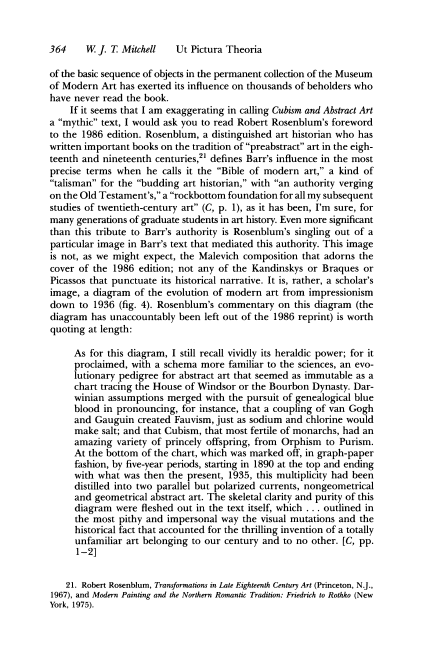
\includegraphics[width=0.9\linewidth]{./images/quotations-01.png}}
\caption{Many books have quotes flushed right.}
\label{frightquotation}
\end{figure}

\begin{figure}[p]
\centering
\fbox{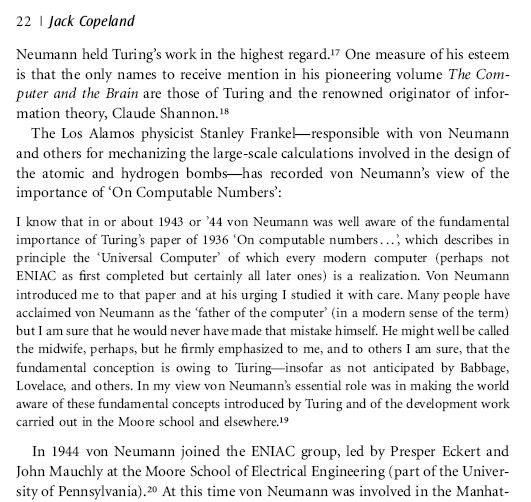
\includegraphics[width=0.9\linewidth]{./images/full-width-quotation.jpg}}
\caption[Sample quotation.]{Other books have the quotations full width, but in smaller font as shown above. the extract is from \textit{The Essential Turing}, Edited by B. Jack Copeland and  published by the Oxford University Press, 2004. }
\label{fullwidthquotation}
\end{figure}


\section{Quotation}

In the standard \LaTeXe\ classes the quotation and quote environment are defined by making use of the list environment. The main difference between the quotation and the quote environment is that the first line of the former is indented. The key value interface for the quotation environment is shown below and a similar one exists for the quotation environment:


\let\quotation\oquotation
\begin{quotation}
\lipsum[1]
\end{quotation}

The standard classes offer a very similar enevironment with the only difference the first line is not indented and is illustrated below:

\begin{quote}
\lipsum[1]
\end{quote}


\section{Key-value interface}\index{quotation!keys}


\begin{key}{/phd/ quote above = \meta{dim}} The space to leave at the top of the quote environment. This is a skip dimension. 
\end{key}

\begin{key}{/phd/ quote below = \meta{dim}} The space to leave at the bottom of the quote environment. This is a skip dimension. 
\end{key}
\begin{key}{/phd/ quote parindent = \meta{dim}} The paragraph indentation, set to 0pt for the quote environment by
\latex.
\end{key}
\begin{key}{/phd/ quote parsep = \meta{dim}} The paragraph separation, normally set to 1pt.
\end{key}
\begin{key}{/phd/ quote left margin = \meta{dim}} The indentation from the left margin.
\end{key}
\begin{key}{/phd/ quote right margin = \meta{dim}} The indentation from the right margin.
\end{key}

\begin{key}{/phd/ quote font-name = \meta{fontcmd}} Set a different font. Defaults to document 
\end{key}
\index{quotation!example}
\begin{tcblisting}{title=Quotation environment example,width=\textwidth}
\bgroup
\setquotation{%
  quotation above=36pt,
  quotation left margin=30pt,
  quotation right margin=0pt,
  quotation parsep=10pt,
  quotation font-size=,
  quotation parindent=1em,
  quotation font-name=\arial,
}
\lorem

\begin{quotation}
\lipsum[2-3]
\end{quotation}
\egroup
\end{tcblisting}

\section{Quote}
This is the quote environment:
\begin{quote}
\lipsum[1-2]
\end{quote}


\section{Some commonly used styles}

Besides the centered quotation \fref{fullwidthquotation} shows a style
common in Oxford University Publications. This one is from \textit{The Essential Turing}, Edited by B. Jack Copeland and  published by the Oxford University Press, 2004. Perhaps indicative of the efforts of academic publications to keep costs down quotations are set at full width, but in smaller font. They both look good and keep the cost down by reducing the amount of paper required to print the book.

\topline

Von Neumann gave his engineers `On Computable Numbers' to read when, in
1946, he established his own project to build a stored-programme computer at
the Institute for Advanced Study.\textsuperscript{22} Julian Bigelow, von Neumann's chief engineer,
recollected:
\vspace*{-20pt}

\cxset{quotation example/.style={
  quotation above=0pt,
  quotation left margin=0pt,
  quotation right margin=0pt,
  quotation parsep=10pt,
  quotation font-size=\small\color{blue},
  quotation parindent=1em,
  quotation font-name=\arial,
}}

\cxset{quotation turing/.style={
  quotation above=0pt,
  quotation left margin=0pt,
  quotation right margin=0pt,
  quotation parsep=10pt,
  quotation font-size=\small,
  quotation parindent=1em,
  quotation font-name=\pan,
}}

\cxset{quotation theme/.code = \setquotation{quotation #1},
       quotation style/.code = \setquotation{quotation #1}}



\cxset{quotation theme = example}
\begin{quotation}

The person who really\ldots pushed the whole Weld ahead was von Neumann, because he
understood logically what [the stored-programme concept] meant in a deeper way than
anybody else\ldots The reason he understood it is because, among other things, he understood
a good deal of the mathematical logic which was implied by the idea, due to the
work of A. M. Turing\ldots in 1936-1937\ldots Turing's [universal] machine does not sound
much like a modern computer today, but nevertheless it was. It was the germinal
idea\ldots So\ldots [von Neumann] saw\ldots that \textsc{[ENIAC]} was just the first step, and that great
improvement would come.\textsuperscript{23}
\end{quotation}

\bottomline

Personally I like this style, especially for books that have a lot
of lengthy citations such as typically found in the humanities and
scientific fields.

\section{Theming}

To make things easier for the designer and to enable easy re-use of
styles we defined a theme key. You first define your keys via
the \cs{cxset} command and then you call it normally using the 
theme. You can extend it, if you like to use sub-themes, such as 
quotation theme |quotation theme = example teal|. 

\begin{teX}
\cxset{quotation example/.style={
  quotation above=0pt,
  quotation left margin=0pt,
  quotation right margin=0pt,
  quotation parsep=10pt,
  quotation font-size=\small,
  quotation parindent=1em,
  quotation font-name=\arial,
}}
\cxset{quotation theme = example}
\end{teX}

\cxset{quotation font-size=\large,
       quote font-size=\large}








% \cxset{steward,
  numbering=arabic,
  custom = stewart,
  offsety=0cm,
  image=hine06,
  texti={A picture is worth a thousand words, but if you don't add a good description of what it is in a caption, your readers will be left scratching their heads. Here we discuss captions in general as well as the formatting commands available in LaTeX, some common packages and athena.},
  textii={In this chapter we discuss methods that allow the formatting and positioning of captions, based on a set of key values. Central  to this process is the separation of content from presentation.
We also discuss the basic formatting tools that are available and how one can modify them to blend them with the rest of the design.
 }
}
\chapter{Typesetting Captions}
\section{Introduction}

Publications that include figures and tables will normally dictate
the style of captions. Captions, besides normal typography 
requirements such as fonts, can vary in their numbering scheme, can
include a label such as figure or fig they can include a colon or stop
after the label and can be centered hanged or left justified. 
Numbering can also vary; the counters can be reset at every chapter or section or can be continuous. So
there are quite a few options to define in a template.

The formatting commands for the captions key value interface follow the same style of the rest of the package. We use the \pkg{caption} package to provide the interface to the key value settings.


\section{Conventions}

All caption keys start with the word |caption|. The float type follows, so |caption figure font-size| refers to the caption of a \textit{figure environment}. If the word \textit{figure} is omitted the style is applicable to both tables and figures. 

As users will probably only have to set these keys once, my recommendation is to use the longer version that can give you finer control. Also your template will be easier to modify in the future.
\medskip

\keyval{caption format}{\marg{plain|hang}}{This affects all captions such as tables and figures and will produce either a hang caption or with plain will wrap arund the figure number like a normal paragraph.}

\keyval{caption figure format}{\marg{plain | hang}}{Affects ONLY figure captions such as tables and figures and will produce either a hang caption or with plain will wrap around the figure number like a normal paragraph.}

\keyval{caption figure numbering style}{\marg{auto|continuous|reset on sections|custom}}{}
\keyval{caption figure numbering}{arabic,alph,Alph,roman,Roman,custom}{}
\keyval{caption separator}{colon,semicolon,none,custom}{Sets the separator, such as \textbf{:} or a colon or none.}
\keyval{caption label name}{}{}
\keyval{caption before}{}{}
\keyval{caption after}{}{}

\cxset{caption format/.code=\captionsetup[figure]{format=#1}}


\begin{texexample}{}{}
\bgroup
\cxset{caption format = hang}
\captionof{figure}{This is a very long command to see how all
these can wrap in a hang format, if the text is longer than
a paragraph.}
\egroup

\bgroup
\cxset{caption format = plain}
\captionof{figure}{This is a very long command to see how all
these can wrap in a hang format, if the text is longer than
a paragraph.}
\egroup
\end{texexample}

As you can see from the example, the changes can also be localized if
they are within a group.



\def\captionlabelfont@cx{bf}
\cxset{caption font/.code = \captionsetup[figure]{font=#1}}

\cxset{caption font={bf}}




\begin{texexample}{}{}
\cxset{caption format = hang}
\cxset{caption font={bf}}
\captionof{figure}{This is a very long command to see how all
these can wrap in a hang format, if the text is longer than
a paragraph.}
\end{texexample}



\section{Technical discussion}

The formatting of the caption, happens in stages like the sectioning commands.  \lstinline+\@makecaption}+  command is responsible for the typesetting and is defined in the standard LaTeX classes. The \cs{caption} and command is defined in the LaTeX kernel in the 
|float.dtx| class. As always we will start our discussion from the user command and follow it through to the typesetting macros.

When the user command \cs{caption} is processed, LaTeX checks if it is outside a float and if it is issues an error message. It then swallows the argument. It then calls \cs{@caption} which does further processing.


\begin{tcolorbox}
\begin{lstlisting}
\def\caption{%
5 \ifx\@captype\@undefined
6 \@latex@error{\noexpand\caption outside float}\@ehd
7 \expandafter\@gobble
8 \else
9 \refstepcounter\@captype
10 \expandafter\@firstofone
11 \fi
12 {\@dblarg{\@caption\@captype}}%
13 }


\long\def\@caption#1[#2]#3{%
15 \par
16 \addcontentsline{\csname ext@#1\endcsname}{#1}%
17 {\protect\numberline{\csname the#1\endcsname}{\ignorespaces #2}}%
18 \begingroup
        \@parboxrestore
20 \if@minipage
21     \@setminipage
22 \fi
23 \normalsize
24 \@makecaption{\csname fnum@#1\endcsname}{\ignorespaces #3}\par
25 \endgroup}
\end{lstlisting}
\end{tcolorbox}

The \cs{@makecaption} is the main typesetting macro and this is
where we need to hook if we want finer grain of control.


\cxset{label punctuation/.code = \gdef\labelpunctuation@cx{#1}}
\cxset{label space/.code = \gdef\labelhspace@cx{\hskip#1}}

\captionof{figure}{This is a very long command to see how all
these can wrap in a hang format, if the text is longer than
a paragraph.}

\begin{texexample}{}{}

\cxset{caption format = hang}
\cxset{caption font={tt}}
\cxset{label punctuation=?}
\cxset{label space =1.5em}

\captionof{figure}{This is a very long command to see how all
these can wrap in a hang format, if the text is longer than
a paragraph.}

\end{texexample}


\cxset{label punctuation=?}
\captionof{figure}{This is a very long command to see how all
these can wrap in a hang format, if the text is longer than
a paragraph.}

\cxset{label punctuation=:}
\cxset{label space =.5em}
\def\figurename{\textbf{Figure}}

\setlength\abovecaptionskip{10\p@}
\setlength\belowcaptionskip{0\p@}

\long\def\@makecaption#1#2{%
  \vskip\abovecaptionskip
  \sbox\@tempboxa{#1\labelpunctuation@cx #2}
  \ifdim \wd\@tempboxa >\hsize
    #1\labelpunctuation@cx\labelhspace@cx#2\par
  \else
    \global \@minipagefalse
    \hb@xt@\hsize{\hfil\box\@tempboxa\hfil}%
  \fi
  \vskip\belowcaptionskip}

\begin{tcolorbox}
\begin{lstlisting}
\newlength\abovecaptionskip
\newlength\belowcaptionskip
\setlength\abovecaptionskip{10\p@}
\setlength\belowcaptionskip{0\p@}

\long\def\@makecaption#1#2{%
  \vskip\abovecaptionskip
  \sbox\@tempboxa{#1:: #2}
  \ifdim \wd\@tempboxa >\hsize
    #1:: #2\par
  \else
    \global \@minipagefalse
    \hb@xt@\hsize{\hfil\box\@tempboxa\hfil}%
  \fi
  \vskip\belowcaptionskip}
\end{lstlisting}
\end{tcolorbox}

\section{List of Figures}
\begin{tcolorbox}
\begin{lstlisting}
\newcommand\listoffigures{%
    \if@twocolumn
      \@restonecoltrue\onecolumn
    \else
      \@restonecolfalse
    \fi
    \chapter*{\listfigurename}%
      \@mkboth{\MakeUppercase\listfigurename}%
              {\MakeUppercase\listfigurename}%
    \@starttoc{lof}%
    \if@restonecol\twocolumn\fi
    }
\end{lstlisting}
\end{tcolorbox}


In the |phd| package this is set as a property via a key-value interface and hence we can use a normal chapter. If it need be we can define a special chapter style only for this heading. This way we can control all aspects of the formatting of the head.

\begin{macro}{\listfigurename}
The \textit{List of Figures} for example in many Social Sciences books is typed as {List of Illustrations} and also adds credits.
\end{macro}




\begin{figure}[htp]
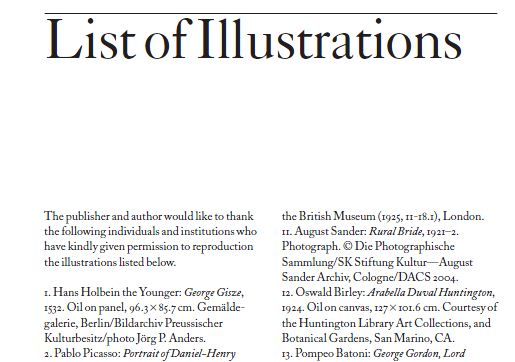
\includegraphics[width=\textwidth]{listofillustrations}
\caption{List of Illustrations extract from \textit{Oxford History of Art, Portraiture}, Shearer West, Oxford University Press, 2004.}
\end{figure}
\begin{figure}[htp]
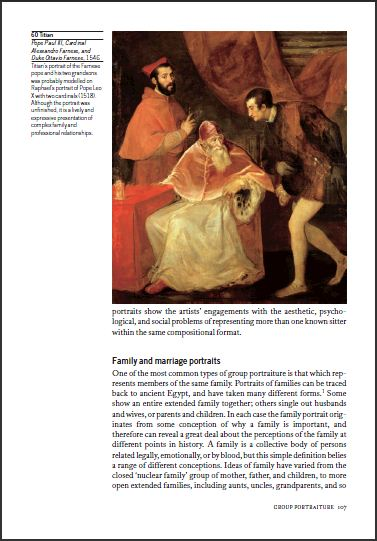
\includegraphics[width=0.67\textwidth]{titian}
\centering
\caption{Figure from \textit{Oxford History of Art, Portraiture}, Shearer West, Oxford University Press, 2004. The figures are numbered consecutively and the text in the List of Illustrations have different formatting.}
\end{figure}

\section{Formatting the List of Figures Heading}

LaTeX formats the list of figures heading in a similar manner to that of the Table of Contents. The Title `List of Figures` is obtained from the \cs{listfigurename} and which is also accessible from Babel. It does not add an entry to the ToC.



It is good to know that \cs{captionsetup} has an effect on the current environment only.
So if you want to change settings for the current figure or table only, just place the
\cs{captionsetup} command inside the figure or table right before the \cs{caption}
command.


Many of the caption figures can be changed within LaTeX itself. For example to get continuous numbering in the book class.

\begin{tcolorbox}
\begin{lstlisting}
\makeatletter
\@removefromreset{table}{chapter}
\renewcommand{\thetable}{\arabic{table}}
\makeatother
\end{lstlisting}
\end{tcolorbox}

\begin{macro}{removefromreset}
The command \cs{removefromreset} can be found by loading the \pkg{remreset} package. Other combinations are also possible.
\end{macro}

\subsection{Caption numbering scheme}

The caption numbering scheme key value interface, provides five
options: 
\medskip

\keyval{caption numbering scheme}{\marg{default|continuous| chapter|section}}{The numbering style either continous or reset per spacing etc...}


% Date: Sat, 30 Jul 1994 17:58:55 PST
% From: Donald Arseneau <asnd@erich.triumf.ca>
%
%  |\@removefromreset{FOO}{BAR}| : Removes counter FOO from the list of
%                       counters |\cl@BAR| to be reset when counter BAR
%                       is stepped.  The opposite of |\@addtoreset|.

\def\@removefromreset#1#2{\let\@tempb\@elt
   \expandafter\let\expandafter\@tempa\csname c@#1\endcsname
   \def\@elt##1{\expandafter\ifx\csname c@##1\endcsname\@tempa\else
         \noexpand\@elt{##1}\fi}%
   \expandafter\edef\csname cl@#2\endcsname{\csname cl@#2\endcsname}%
   \let\@elt\@tempb}

\@removefromreset{figure}{chapter}
\renewcommand{\thefigure}{\arabic{figure}}

\@specialfalse\@tocfalse

\begin{texexample}{}{}
\setdefaults
\cxset{chapter opening=anywhere,
          chapter font-size=\normalfont,
          title font-size=\large}


\gdef\continuousfigures@cx{\@removefromreset{figure}{chapter}
\gdef{\thefigure}{\arabic{figure}}}

\cxset{caption numbering continuous/.code={\continuousfigures@cx}}


\chapter{This is the First Chapter}
\captionof{figure}{test}
\captionof{figure}{test}
\chapter{This is the Second Chapter}
\captionof{figure}{test}
\captionof{figure}{test}
\end{texexample}


\begin{figure}[htp]
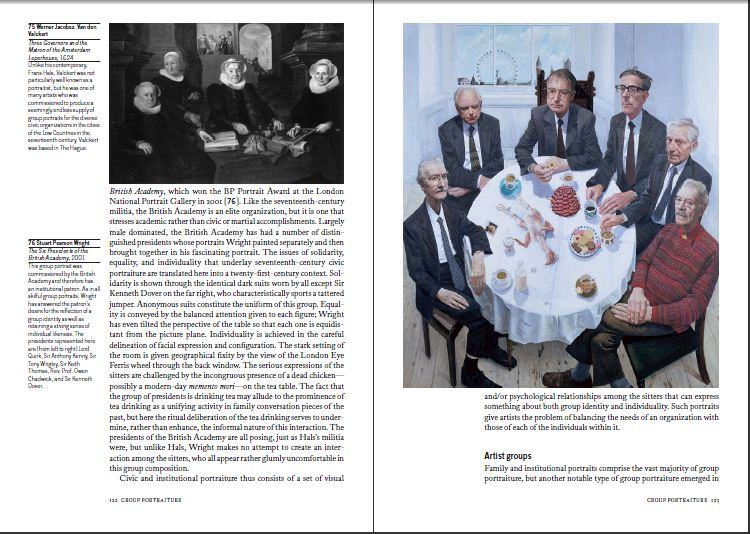
\includegraphics[width=0.98\textwidth]{captionspecial}
\centering
\caption{Figure from \textit{Oxford History of Art, Portraiture}, Shearer West, Oxford University Press, 2004. The figures are numbered consecutively and the text in the List of Illustrations have different formatting.}
\end{figure}



% 
\cxset{lineskip/.code=\setlength\lineskip{#1},
       lineskip/.default=1pt,
          normallineskip/.code=\setlength\normallineskip{#1},
          parindent/.code=\setlength\parindent{#1},
          parskip/.code=\setlength\parskip{#1},
          text-indent/.code=\setlength\parindent{#1},
          baselinestretch/.code=\renewcommand\baselinestretch{#1},
          single spacing/.code=\singlespacing,
          single spacing/.default=\singlespacing,
          double spacing/.code=\doublespacing}

\cxset{lineskip=1pt,
          normallineskip=1pt,
          parindent=1em,
          parskip=1pt,
          text-indent=1em,
          baselinestretch={},
          single spacing}

\makeatletter\@specialtrue\makeatother
\cxset{steward,
  numbering=arabic,
  custom=stewart,
  offsety=0cm,
  image={./images/hine05.jpg},
  texti={When Lamport designed the original \LaTeX\ sectioning commands, limitations of computer power forced him to restrict the abstraction of complicated chapter layouts. With current tools available improvements are much easier to program.},
  textii={In this chapter we discuss a method that allows the production of fancy chapter headings and formatting, based on a set of key values. Central  to this process is the separation of content from presentation.
We also discuss the basic formatting tools that are available and how one can modify them to mould new book designs.
 }
}
\cxset{chapter opening=left}

\chapter{General Settings}

\section{Introduction}

Here we define and set general paragraph settings. The parameters which control \TeX's behaviour when typesetting paragraphs can receive a bit of a tweak here. We also describe a set of options to handle parameters that can influence grid typesetting. This is especially important for two or more column typesetting. The commands act only on the text within a grouped environment. They do not affect captions or footnotes. Use anything over \emph{single spacing} with care, as books are meant to be single spaced.  



\section{Controlling inter-line spacing}
\index{line spacing}
Interline spacing traditionally has been controlled using the \pkgname{setspace} or by setting appropriate primitive \tex commands. The \pkgname{phd} loads the |setspace| package and then provides parameterized commands for setting styles. 

\begin{key}{/chapter/single spacing} 
	The Lineskip parameter emulates \TeX's \cmd{\parindent} command.
\end{key}
\begin{key}{/chapter/one half spacing} 
	The Lineskip parameter emulates \TeX's \cmd{\parindent} command.
\end{key}
\begin{key}{/chapter/double spacing} 
	Sets the document line-spacing to double.
\end{key}

If you want to use larger inter-line spacing in a document, you can change its value by putting the

\CMDI{\linespread}\meta{factor} Use |\linespread{1.3}| for "one and a half" line spacing, and |\linespread{1.6}| for "double" line spacing. Normally the lines are not spread, so the default line spread factor is~1.

The setspace package allows more fine-grained control over line spacing. To set "one and a half" line spacing document-wide, but not where it is usually unnecessary (e.g. footnotes, captions):

\begin{teXXX}
\usepackage{setspace}
%\singlespacing
\onehalfspacing
%\doublespacing
%\setstretch{1.1}
\end{teXXX}

The |phd| package provides the settings

\begin{key}{/chapter/single spacing}
We use the \pkgname{setspace} to effect the desired line spread effect.
\end{key}


These command offer little value over the normal \TeX\ macros other than keeping the interface, uniform. One can also extend the interface to cover CSS style commands:

\begin{verbatim}
\cxset{text-indent=50pt}

\cxset{double spacing}
\lipsum*[1]

\cxset{single spacing}
\lipsum*[1]
\end{verbatim}



\subsection{Parameters controlling paragraphs}\index{Paragraphs!controlling parameters}
The parameters \cs{lineskip} and \cs{normallineskip} influence \TeX\ when two lines come two close.
\medskip



\begin{key}{/chapter/lineskip=1pt} 
	The Lineskip parameter emulates \TeX's \cmd{\lineskip} command.
\end{key}

\begin{key}{/chapter/normallineskip=\marg{dim}} 
	The normallineskip parameter emulates \TeX's \cmd{\normallineskip} command.
\end{key}

\begin{key}{/chapter/lineskiplimit=\marg{dim}} 
	The Lineskip parameter emulates \TeX's \cmd{\lineskiplimit} command.
\end{key}

\begin{key}{/chapter/parindent=\marg{dim}} 
	The Lineskip parameter emulates \TeX's \cmd{\parindent} command.
\end{key}

\keyval{parindent}{\marg{dim}}{Paragraph indentation.}
\keyval{text-indent}{\marg{dim}}{Alias for \cs{parindent}.}
\keyval{parskip}{\marg{dim}}{Spacing between paragraphs.}


Another advantage, the package offers a few pre-configured styles, just setting a style to latex will revert everything back to latex.

\section{Technical discussion}

Most classes, including the standard \LaTeXe\ classes as well as packages attempting to achieve a grid typesetting try define a text height that is a multiple of \cs{baselineskip}. This way they give little opportunity to TeX to adjust the vertical glue to achieve a flush bottom.

\section{Dropcaps and Lettrines}\index{Lettrine!basic typesetting}

Dropcaps or lettrines are those letters that start paragraphs with a fancy larger letter. The class uses a parameterized version of the lettrine package of Daniel Flipo. Lettrine letters are easily typed and produced, but they are notoriously difficult to get right and no-one seems to agree on settings. These settings depend on the font the sizing of the text and the personal taste of the book interior designer. As I don't profess to be one, I have done what I think Knuth have done (just studied existing sources) allowed programming hooks and provided defaults as close as possible to the originals.



% 
%%% DOCUMENATION MACROS
%% note becareful with styles here

\thispagestyle{plain}
\cxset{image=breakerboys, custom=stewart}
\chapter{Documentation}


\section{Documentation macros}

When developing this package the need arose to define a number of documentation macros. I have used heavily macros and ideas present in the doc package, pgf documentation, biblatex documentation  and tcolorbox and for which I am grateful to their respective authors. The major change was to adopt the macros to use different fonts and colors and to use these from a list of key values defined at document level. More about this later. General package user documentation as opposed to package documentation that can be achieved using the doc/docstrip system requires that macros and environments be developed for the following:

\begin{enumerate}
\item Macros for command documentation.
\item Environments for commands and options.
\item Latex examples that need to be executed within the document as well as described.
\end{enumerate}

\subsection{Color management}
One of the first requirements for redefining some of the standard doc commands is the need to use color easily, hence we will try and define a certain amount of keys for colors.

Just a bit of a refresher, to define colors we use, either the \cs{definecolor} or the \cs{colorlet} commands.

\emphasis{definecolor,colorlet}
\begin{tcolorbox}
\begin{lstlisting}
% used for hyperlinks
\definecolor{Hyperlink}{rgb}{0.281,0.275,0.485}
\colorlet{thehyperlink}{theblue}
\end{lstlisting}
\end{tcolorbox}

We use a semantic approach, where the colors are first defined with a mnemonic command such as {\bfseries\textcolor{theblue}{theblue}} and then we define a semantic command such as the\cs{option} that lets the color to the option command. This sort of double entry has proved useful in navigating through the dozen of the commands that I needed for this documentation.

%\definecolor{theblue} {rgb}{0.02,0.04,0.48}
%\definecolor{thered}  {rgb}{0.65,0.04,0.07}
%\definecolor{thegreen}{rgb}{0.06,0.44,0.08}
%\definecolor{thelightgreen}{rgb}{0.06,0.44,0.06}
%\definecolor{thegrey} {gray}{0.5}
%\definecolor{thegrey} {gray}{0.5}
%\definecolor{theshade}{gray}{0.94}
%\definecolor{theframe}{gray}{0.75}
%\definecolor{thecream}{rgb}{1,0.95,0.4}
%\definecolor{spot}{rgb}{0,0.2,0.6}
%\definecolor{boxframe}{gray}{0.8}
%\definecolor{boxfill}{rgb}{0.95,0.95,0.99}
%\definecolor{theoption}{rgb}{0.118,0.546,0.222}
%\definecolor{themacro}{rgb}{0.784,0.06,0.176}
%\definecolor{ExampleFrame}{rgb}{0.628,0.705,0.942}
%\definecolor{ExampleBack}{rgb}{0.963,0.971,0.994}
%\definecolor{Hyperlink}{rgb}{0.281,0.275,0.485}
%\colorlet{thehyperlink}{theblue}
%\newcommand*{\defaultcolor}{\color{black}}
%\newcommand*{\spotcolor}{\color{spot}}

\subsection{Semantic color names}
\begin{marglist}
\item [\option{theoption}] Coloring of options in margin lists.
\item [\option{themacro}] Coloring of command macros \cs{foo}.
\item [\option{hyperlink}] If we use the \texttt{hyperref} package a number of colors need to be defined for links.
\end{marglist}

\subsection{Named colors}
Standard colors that we provide are:
\begin{marglist}
\item [\textcolor{theblue}{theblue}] This color is used mainly for options.
\item [\textcolor{thered}{thered}] The color mostly used for macro commands and keys.
\item [\textcolor{thegreen}{thegreen}] used for environments.
\item [\textcolor{thelightgreen}{thelightgreen}] Used for margin lists.
\item [\textcolor{thegray}{thegray}] Used as a background to the listings.
\item [\colorbox{thegrey}{\color{white}thegrey}] Alias for the gray to satisfy both sides of the Atlantic and as I sometimes don't remeber which is which.
\item [\colorbox{theshade}{theshade}] Another slightly lighter shade.
\end{marglist}



\begin{marglist}
\item [\cs{cs}] \cs{cs}\marg{text} Prints a command.
\item [\cs{cmd}] \cmd{\cmd}\marg{\cmd{\foo}} Prints a command.
\item[\cs{meta}] \marg{macro|text} Prints an argument
\end{marglist}




\section{Lists for documentation}



The environment \env{marglist}
\begin{marglist}
\item[testing]\lorem
\item [test]\lorem
\end{marglist}

\env{keymarginlist}This environment is suitable for listing keys, set-in the margin.

\begin{keymarglist}
\item[bibliography] The term <bibliography>, also available as \cmd{bibname}.
\item[references] The term <references>, also available as \cmd{refname}.
\item[shorthands] The term <list of shorthands> or <list of abbreviations>, also available as \cmd{losname}.
\end{keymarglist}


\env{argumentlist} This environment is suitable for listing macro arguments and their explanations.

\newenvironment*{argumentlist}[1]
  {\list{}{%
     \settowidth{\labelwidth}{\displayverbfont#1}%
     \setlength{\labelsep}{1em}%
     \setlength{\leftmargin}{\labelwidth}%
     \addtolength{\leftmargin}{\labelsep}%
     \setlength{\itemsep}{0pt}%
     \renewcommand*{\makelabel}[1]{\displayverbfont##1\hss}}}
  {\endlist}

\begin{argumentlist}{00}
\item[\#1] The last names. If a name consists of a single part only (for example, <Aristotle>), this part will be treated as the last name.
\item[\#2] The last names, given as initials.
\item[\#3] The first names. This argument also includes all middle names.
\end{argumentlist}

\begin{tabular}{ll}
\env{marglist} & description list\\
\end{tabular}


\section{Future improvements}

Future improvements will involve defining additional environments and styles to integrate styles to those provided for chapters. Treat the code so far as a proof of concept experiment. It is also possible to improve on the code by utilizing some of the common packages.


% \cxset{toc image=false},

\long\gdef\versochapter#1{%
  \vspace*{3cm}
  \minipage{\textwidth}
  \hfill\includegraphics[width=0.63\textwidth]{\chapterimage@cx}\par
  \vspace*{6pt}
  \hfill\minipage{0.75\textwidth}
  {\HUGE\bfseries\flushright #1\endflushright}
  \endminipage
  \endminipage
  \newpage


\vspace*{10cm}
\@specialfalse
\@openleftfalse
\@openanyfalse
\@openrighttrue
}


\newgeometry{bottom=2.5cm}

\cxset{
   chapter image/.code={\def\chapterimage@cx{#1}},
   chapter opening/.is choice,
   chapter opening/verso/.code={\@specialtrue\@openlefttrue
   \gdef\customdesign@cx##1{\versochapter{##1}}}
}

\cxset{
 chapter image=onesowndeath,
 chapter opening=verso,
 name={},
 numbering=none,
 number font-size=\LARGE,
 number font-family=\rmfamily,
 number font-weight=\bfseries,
 number before=,
 number dot=,
 number after=,
 number position=leftname,
 chapter font-family=\sffamily,
 chapter font-weight=\normalfont,
 chapter font-size=\Large,
 chapter before={\vspace*{0pt}\par},
 chapter after={\hfill\hfill\par},
 chapter color={black!90},
 number color=\color{purple},
 title beforeskip={\vspace*{0pt}},
 title afterskip={\vspace*{0.4\textheight}\par},
 title before={},
 title after={},
 title font-family=\sffamily,
 title font-color=\color{purple},
 title font-weight=\bfseries,
 title font-size=\LARGE,
 header style=plain,
 pagestyle=plain,
 }

\@specialtrue

\chapter[VERSO CHAPTERS]{Verso Chapters}

\parindent1.5em
{\HUGE V}erso chapter openings are not common. One design that I found quite attractive is \lipsum[1-3] \textit{From Western attitudes toward death from the middle ages to the present}, Philippe Ari\'es. London, 1974.

\begin{figure}
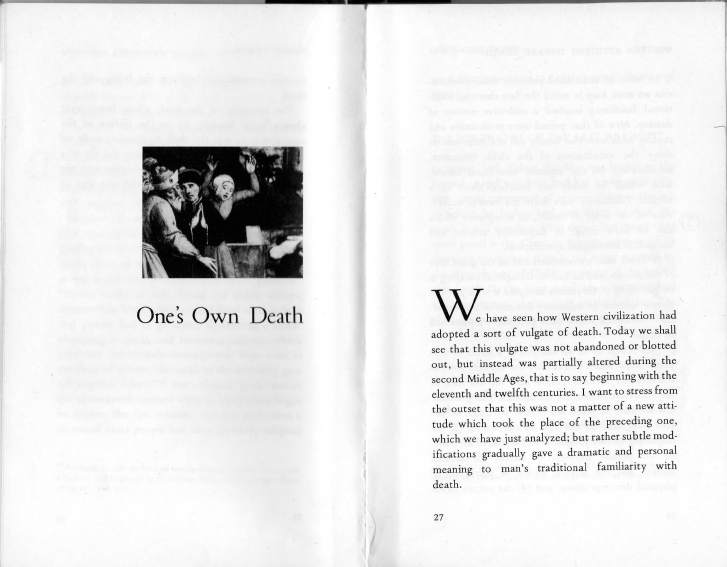
\includegraphics[width=\textwidth]{versochapter01}
\caption{Chapter opening on verso page.}
\end{figure}


^^A \@specialfalse


\newgeometry{top=1.35cm,bottom=2cm,left=2cm}
\clearpage
\cxset{manet/.style={
 chapter opening=anywhere,
 chapter toc=true,
 toc image=false,
 name={},
 numbering=none,
 number font-size=,
 number font-family=,
 number font-weight=,
 number before={\vspace*{-2.5cm}},
 number dot={},
 number after={},
 number position=leftname,
 chapter font-family=,
 chapter font-weight=,
 chapter font-size=,
 chapter before=,
 chapter after={},
 chapter color={black!90},
 number color= teal,
 title beforeskip={},
 title afterskip={},
 title before={\hspace*{-2.47cm}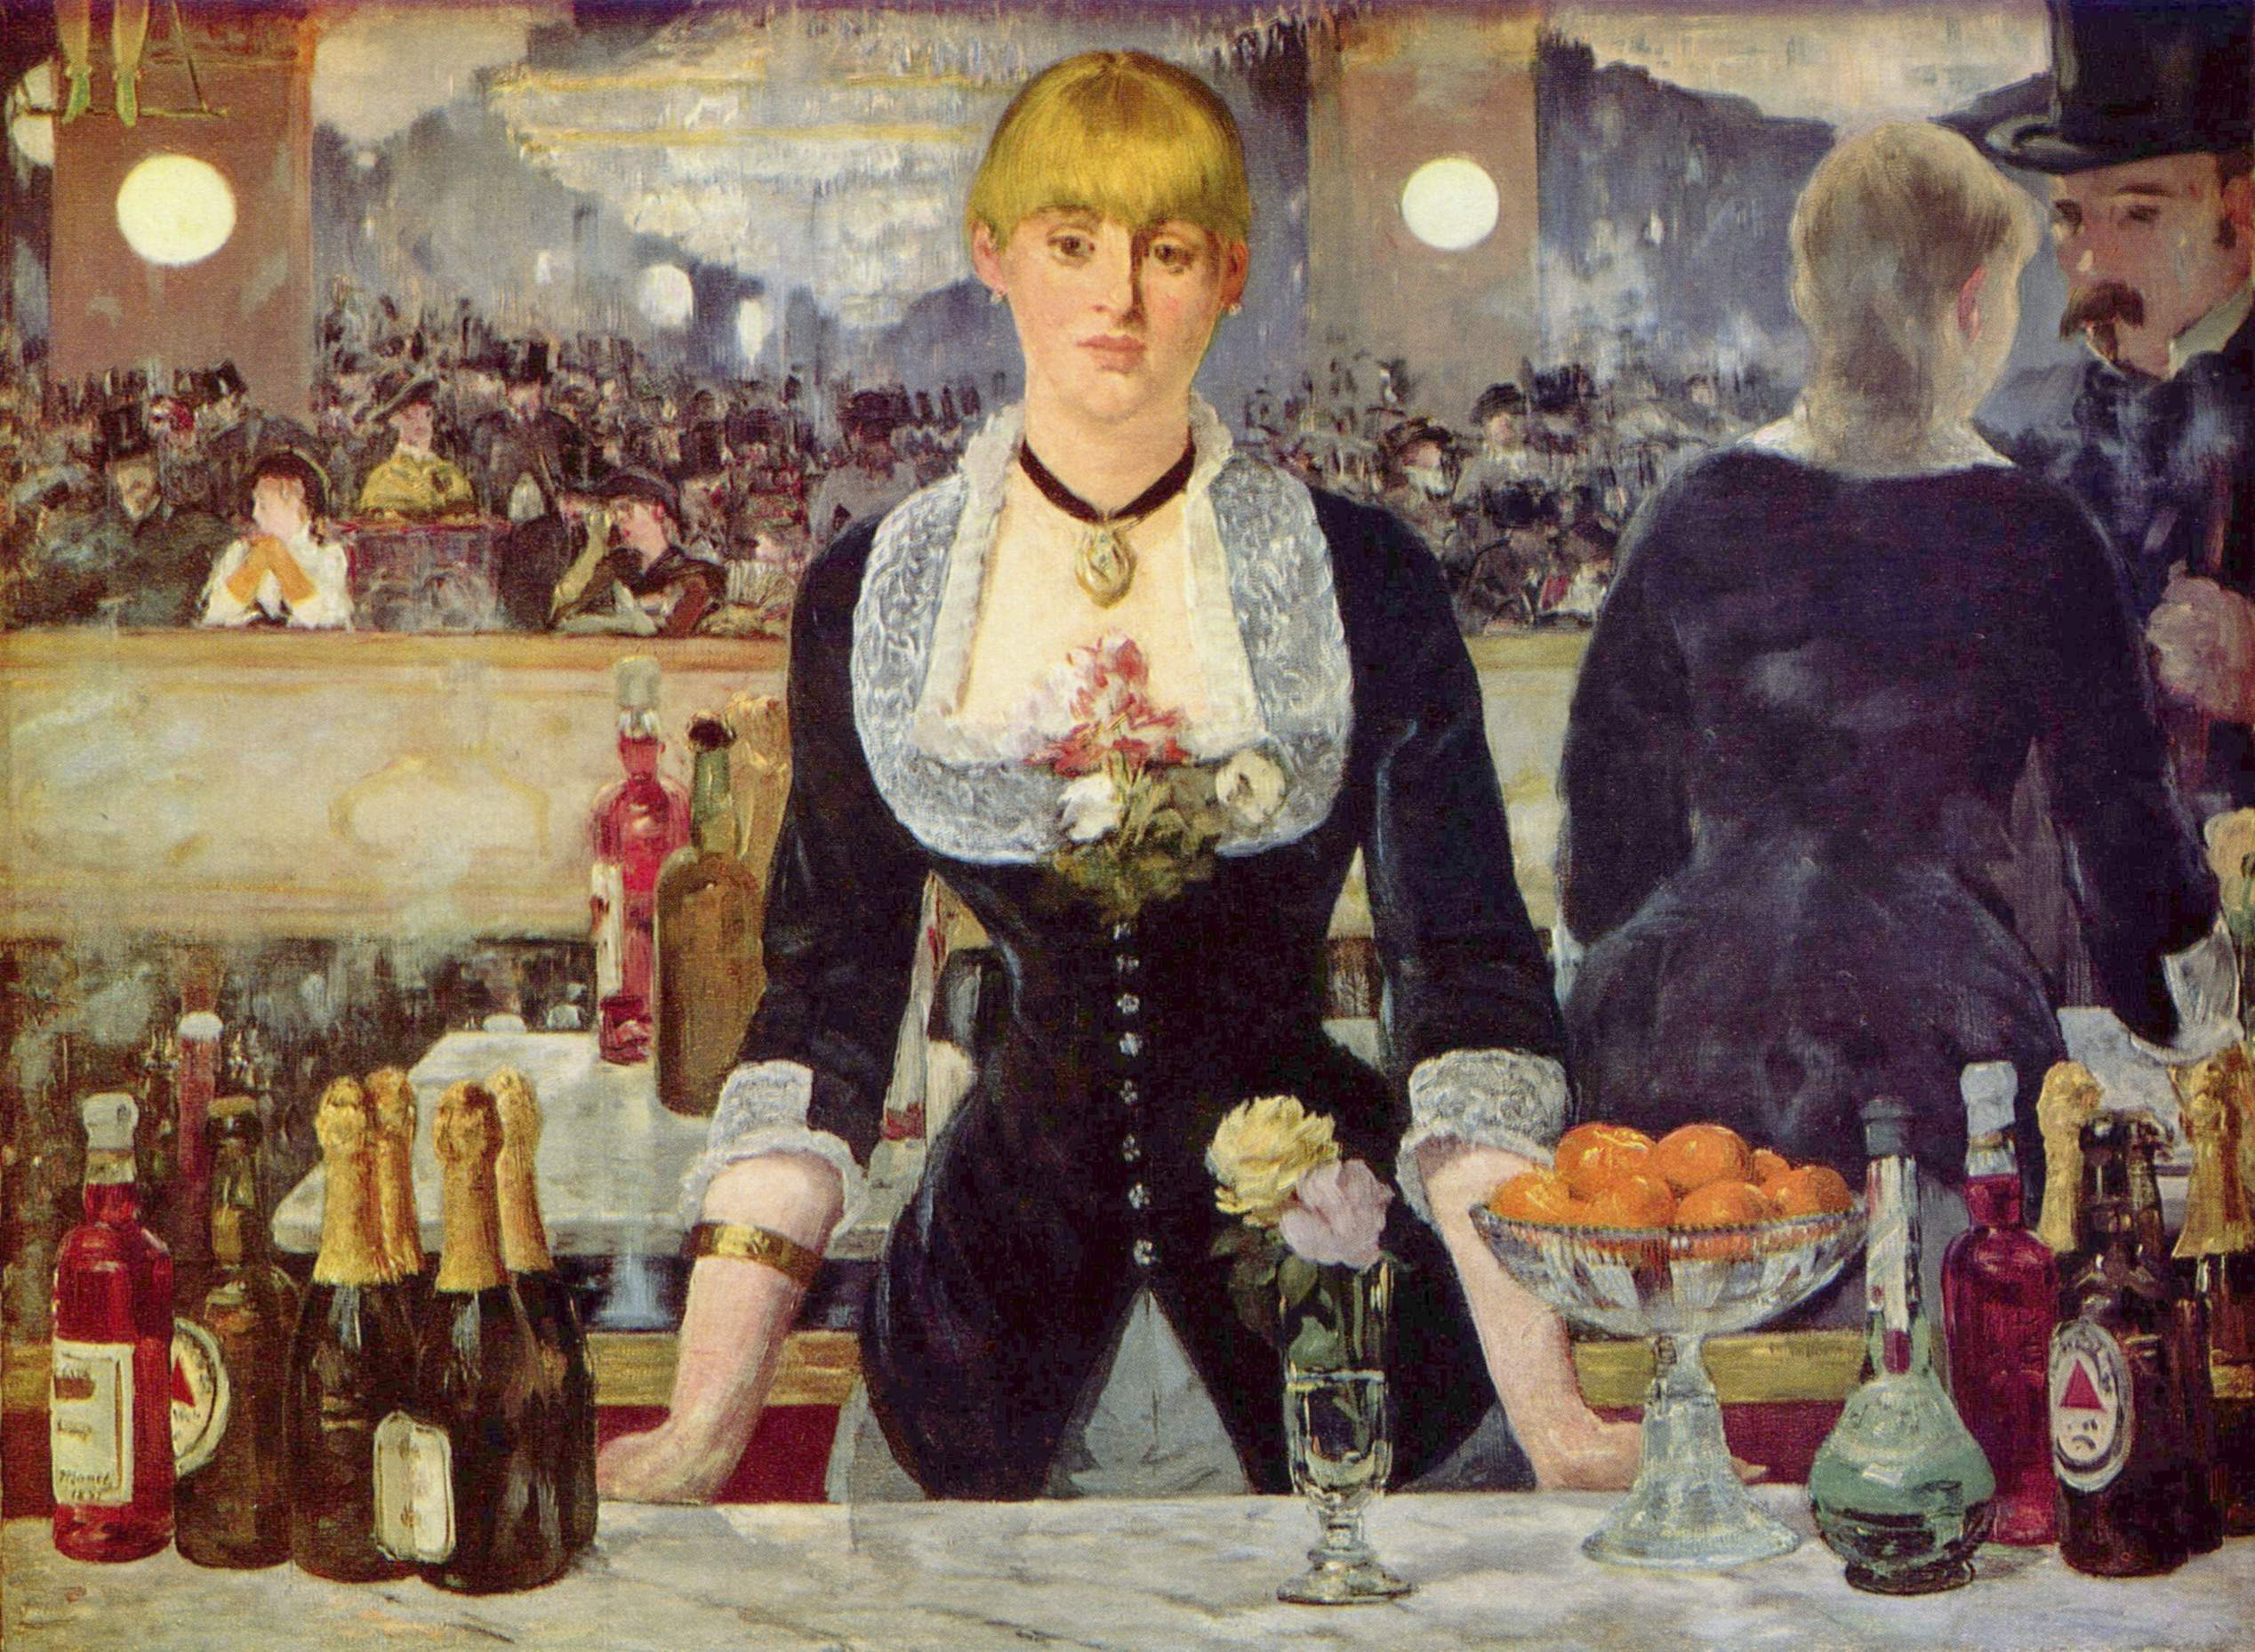
\includegraphics[width=1.27\textwidth]{./chapters/manet}%
    \par\hfill\hfill{\tiny\bfseries Manet's  \textit{The Barmaid.}}\\
    \par
    \vspace*{\baselineskip}
    \par\hfill},
 title after={\hfill\hfill},
 title font-family=\sffamily,
 title font-color= black!80,
 title font-weight=\bfseries,
 title font-size=\LARGE}}
\cxset{manet}



\chapter{A New Approach to Designing \LaTeX\ Classes}
\begin{multicols}{3}
      \leftskip0pt
      \lettrine{I}{psum dolor} sit amet latixeus. \lipsum*[1-2]
      Latinicus porcupinus to fill the line.


This particular code, uses the predefined style \textit{manet}. The only difference we have now defined a helper macro to make it easier for such images to be inserted for similar style chapter openings.
If a full book is to be designed using chapter openings in this fashion more keys and styles could be defined to make it even more easy to enter.
\end{multicols}



\def\topimage#1{\cxset{title before={\hskip-2.3cm\includegraphics[width=1.25\textwidth]{./chapters/#1}\par
\vspace*{\baselineskip}\par}}}




The full code to have the chapter typeset is shown below:


\begin{lstlisting}
\cxset{manet}
\topimage{Alan-MacDonald-Cardinal-Spin-01}

\chapter{ALAN MacDONALD}
\begin{multicols}{3}
      \leftskip0pt
      \lettrine{I}{psum dolor} sit amet latixeus. \lipsum*[1-2]
      Latinicus porcupinus to fill the line.
\end{multicols}
\end{lstlisting}
\lipsum[2]

\loadgeometry{std}



% \makeatletter\@specialfalse

\cxset{
 toc image = \@empty,
 name={},
 numbering=arabic,
 number font-size= LARGE,
 number font-family= rmfamily,
 number font-weight= bfseries,
 number before=,
 number dot=,
 number after=,
 number position=leftname,
 chapter font-family= sffamily,
 chapter font-weight= normalfont,
 chapter font-size= Large,
 chapter before={\vspace*{15pt}\par},
 chapter after={\hfill\hfill\par},
 number color=black!90,
 title beforeskip={\vspace*{30pt}},
 title afterskip={\vspace*{40pt}\par},
 title before={},
 title after={},
 title font-family= sffamily,
 title font-color= black,
 title font-weight= bfseries,
 title font-size= LARGE,
 header style= plain,
 }

\cxset{headings ruled-01}

\chapter{Introduction to Style One}


\begin{summary}
This design is simple and its distinguishing characteristic is a short summary at the beginning of the chapter. This is almost like an abstract typeset in italic font without setting the margins in. We provide a \lstinline{summary} environment for convenience. Note the very simple line in the running head to the left of the page number.
\end{summary}

\medskip
\begin{figure}[ht]
\centering
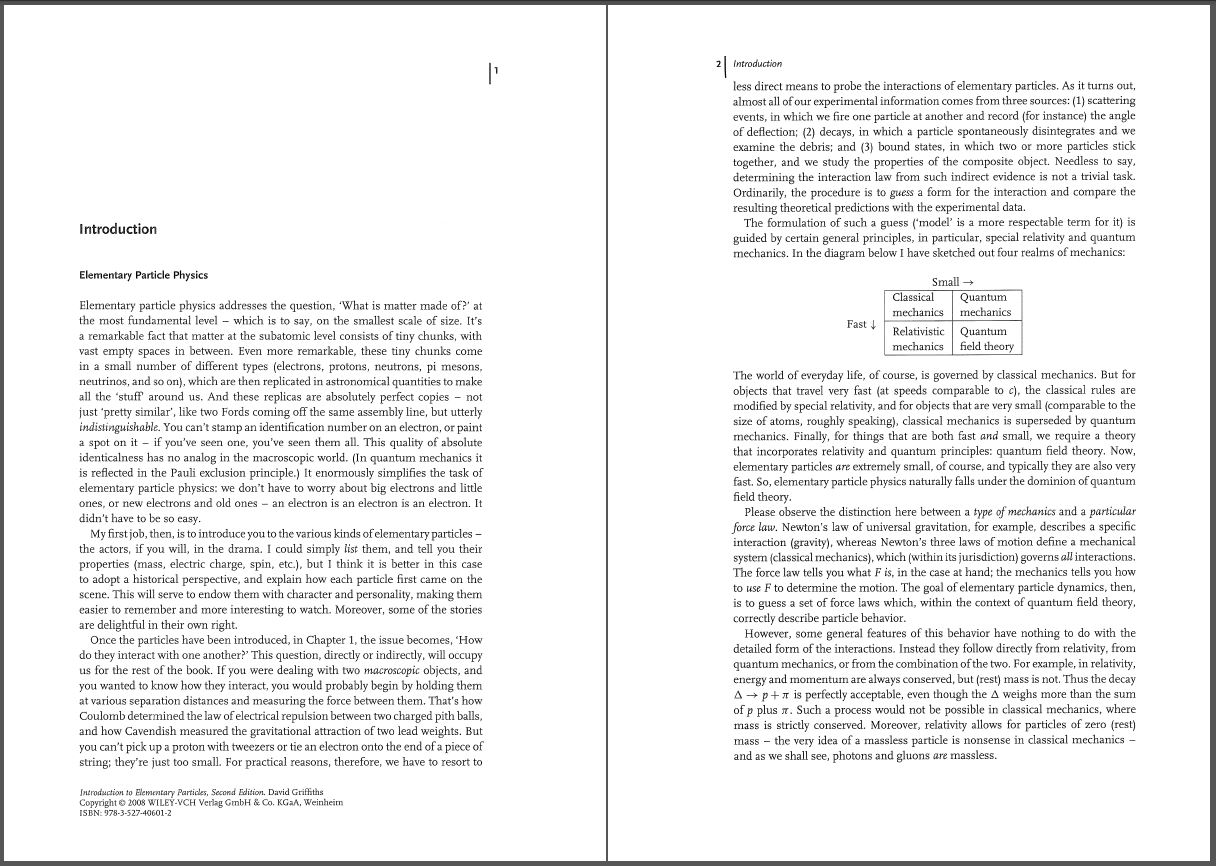
\includegraphics[width=0.5\textwidth]{./chapters/chapter01.png}
\end{figure}
\makeatother

% \clearpage
\makeatletter\@debugtrue\makeatother
\cxset{
 chapter toc=true,
 name=CHAPTER,
 chapter numbering=ORDINALS,
 number font-size=Large,
 number font-family=rmfamily,
 number font-weight=bfseries,
 number before=\kern0.5em,
 number dot=,
 number after=\hfill\hfill\par,
 number position=rightname,
 chapter font-family=rmfamily,
 chapter font-weight=bold,
 chapter font-size=Large,
 chapter before={\vspace*{20pt}\par\hfill},
 chapter after=,
 chapter color=black,
 number color=black,
 %
 title margin top=10pt,
 title before=\par\nointerlineskip\hfill,
 title after=\hfill\hfill\par\nointerlineskip,
 title font-family=rmfamily,
 title font-color= black,
 title font-weight=bfseries,
 title font-size=LARGE,
 chapter title width=0.8\textwidth,
 chapter title align=centering,
 title margin-left=0pt,
 author block=false}

\debugtitle
\debugchapter
\chapter[Template 2]{Mondino, the Restorer of Anatomy}

The archive.org is an extraordinary hunting ground  for typographical surprises. On a recent excursion to find some books on Versalius I stubled on a book titled \emph{Andreas Vesalius, the reformer of anatomy} by  Ball, James Moores. It is an old book published in 1910 and has a couple of unusual features. Check the figure below and see if you can identify the challenging feature.

\begin{figure}[ht]
\centering
\includegraphics[width=0.8\textwidth]{versalius}
\caption{J.B. Moore’s \emph{Andreas Versalius, the Reformer of Anatomy} has many unusual features, including chapter numbers using ordinals. }
\end{figure}

\cxset{chapter toc=true,
          chapter opening=anywhere}
          
\chapter{The Template}          
The template is called \emph{Versalius} and is stored under style02. It can be loaded in the normal way using:
\begin{verbatim}
\usepackage[style02]{phd}
\end{verbatim}

I have not reproduced the full extend of the book’s requirements, as some details are quite cumbersome to be automated through \tex. These though can easily be incorporated in a manual way. More about this later.


\section{The Table of Contents}
Another interesting aspect of this book, which is common with many books of its period is the ToC. The ToC shows the full range of the chapter pages, i.e., it is marked as Page 1-16 rather than the common practice nowdays that indicates only the starting page of the chapter. It also has “TABLE OF CONTENTS”  as a heading and not just contents as you would expect from today’s books.

\begin{figure}[ht]
\centering
\includegraphics[width=0.8\textwidth]{versalius-01}
\caption{J.B. Moore’s \emph{Andreas Versalius, the Reformer of Anatomy} has many unusual features, including chapter numbers using ordinals. }
\end{figure}

\section{List of Illustrations}

\begin{figure}[ht]
\centering
\includegraphics[width=0.8\textwidth]{versalius-02}
\caption{J.B. Moore’s \emph{Andreas Versalius, the Reformer of Anatomy} has many unusual features, including chapter numbers using ordinals. }
\end{figure}

\section{The Frontmatter}
As a foreward there is an unumbered chapter called ``Introduction’’. The chapter heading also has a head band.
\begin{figure}[ht]
\centering
\includegraphics[width=0.8\textwidth]{versalius-03}
\caption{J.B. Moore’s \emph{Andreas Versalius, the Reformer of Anatomy} has many unusual features, including chapter numbers using ordinals. }
\label{lettrine}
\end{figure}

\bgroup
\centering
\includegraphics[width=0.7\textwidth]{versalius-headband}

\LARGE\bfseries INTRODUCTION\par
\egroup
\def\dropcapversalius{%
\vbox to 0pt{\vskip6pt\leavevmode\noindent\includegraphics[width=2.39cm]{versalius-dropcap}%
}%
}
\parindent0pt

\hangindent2.6cm \hangafter0
\dropcapversalius \textsc{he dropcap will have to be inserted}, either using the lettrine package or do be achieved via a parshape command and manual entry. You can also write your own macro command using the details we provide under the Paragraphs chapter. On this page I have manually inserted it, as I used an image from the book for the dropcap. If you were to use the template for a full book, it will be then preferable to use

the lettrine package to set the dropcaps. If you observe Figure~\ref{lettrine} carefully, you will notice the first line of theopening paragraph is in small caps. As \tex typesets the full paragraph this is almost an impossible task to achieve through normal \tex commands and in order not to overcomplicate the discussion it can be achieved manually via trial and error. 

\section{Figures}

Most of the figures are wrapped illustrations. A couple are full page figures and bear no caption numbering. One such illustration is shown on page~\pageref{fig:vesalius}. Do note that the List of Illustrations does have the illustrations listed with additional information to that shown in the captions. 

\begin{figure}[p]
\centering
\includegraphics[width=\textwidth]{vesalius}
\centering
ANDREAS VESALIUS\par
(From an old copperplate engraving)\par
\label{fig:vesalius}
\end{figure}







% \newgeometry{top=-10pt,bottom=2cm}


\cxset{style03/.style={
 toc image = \@empty,
 name={},
 numbering=arabic,
 number font-size= HUGE,
 number font-family= rmfamily,
 number font-weight= bfseries,
 number before=\par\vspace*{10pt}\hfill\hfill,
 number dot=.,
 number after=,
 number position=rightname,
 chapter font-family= sffamily,
 chapter font-weight=normalfont,
 chapter font-size= Large,
 chapter before={\hspace*{-2.5cm}\vbox\bgroup%
    \tcbset{width=\paperwidth,boxrule=0pt,right=3cm,arc=0pt}
    \tcolorbox\bgroup\vspace*{20pt}\hfill\hfill},
 chapter after={\par\vspace*{15pt}},
 chapter color=black!90,
 number color= thered,
 title beforeskip={},
 title afterskip={\vspace*{10pt}\par},
 title before={\hfill\hfill},
 title after={\vspace*{60pt}\egroup\endtcolorbox\egroup},
 title font-family=\sffamily,
 title font-color= thered,
 title font-weight=\bfseries\RaggedRight,
 title font-size=\Huge}}

\cxset{style03}

\chapter{Introduction Style Three}

This is not an exact reproduction as I am still thinking as to how to use
specials with the package. You can vary it by setting the tcolorbox settings as well as the geometry settings.
\medskip

\begin{figure}[ht]
\centering
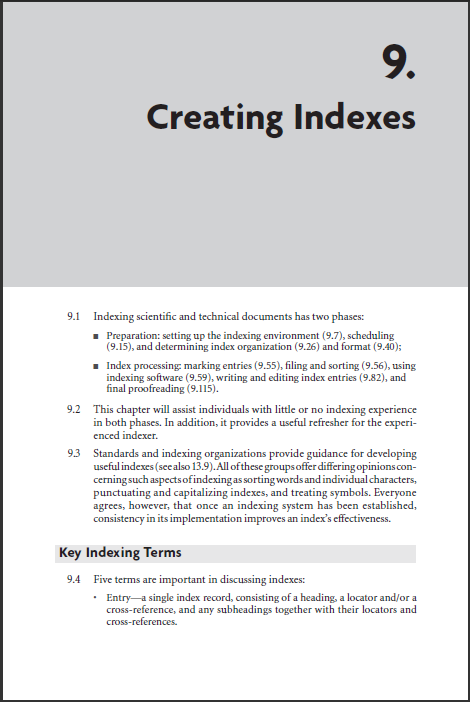
\includegraphics[width=0.39\textwidth]{./chapters/chapter03}
\end{figure}

This setting involves changing the geometry of the page as well as adding the chapter name and title in a color box. For this I have used the \lstinline{tcolorbox}. Of course you can use any other shaded environment you feel comfortable with such as mdframed. It is important to set the colorbox parameters.

\begin{lstlisting}
\newgeometry{top=-10pt}
\tcbset{width=\paperwidth,boxrule=0pt,right=3cm,arc=0pt}
\end{lstlisting}

Note that we set the width of the \lstinline{tcolorbox} to \lstinline{\paperwidth} in order for the shading to extend to the full width of the page.

\restoregeometry

% \cxset{style04/.style={
 chapter name=,
 numbering=Roman,
 number font-size=Large,
 number font-family=rmfamily,
 number font-weight=bfseries,
 number before=,
 number dot=,
 number after=,
 number color=black,
 number position=rightname,
 chapter font-family= rmfamily,
 chapter font-weight=bold,
 chapter font-size=Large,
 chapter before=,
 chapter after=,
 chapter color=black!90,
 chapter border-style=none,
 chapter border-width=0pt,
 chapter display=block,
 chapter float=center,
 title beforeskip={},
% title afterskip={\vspace*{50pt}\par},
 title margin bottom=50pt,
 title margin-left=0pt,
 chapter title align=centering,
 chapter title text-align=center,
 chapter title width=\textwidth,
 title display=block,
 title border-left-width=0.2pt,
% title hooks leave emptt 
 title before=,
 title after=,
 % title families leave as default font name
 title font-family=rmfamily,
  title font-color= black,
 title font-weight=normalfont,
 title font-size=LARGE,
 % title alignment
 chapter title align=centering,
 % sectioning incomplete please add to suit
 section numbering=none,
 section align = center}}

\debugchapter
\cxset{chapter border-width=2pt,
          chapter padding=5pt,
          number border-width=2pt,
          number padding=5pt}

\cxset{style04}

\chapter{INTRODUCTION TO STYLE FOUR}

This is a very simple design applicable perhaps to translations and commentary on older texts.
\medskip
\begin{figure}[ht]
\centering
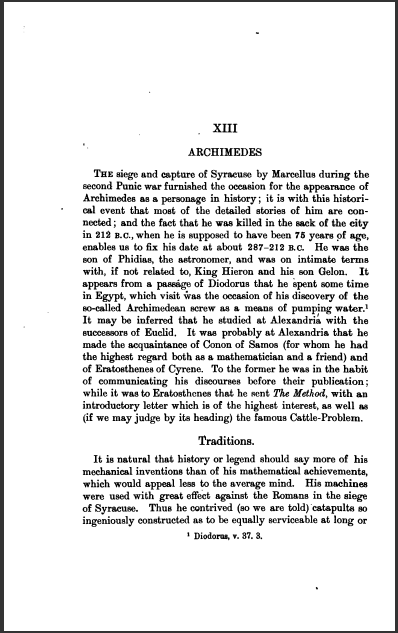
\includegraphics[width=0.6\textwidth]{./chapters/chapter04.png}
\end{figure}

\testsections



% %%%%%%%%%%%%%%%%%%%%%%%%%%%%%%%%%%%%%%%%%%%
%%%%%%  STYLE 05
%%%%%%%%%%%%%%%%%%%%%%%%%%%%%%%%%%%%%%%%%%%


\cxset{style05/.style={
 name={Chapter},
 numbering=arabic,
 number font-size=\Large,
 number font-family=\rmfamily,
 number font-weight=\normalfont\itshape,
 number color=\color{black!90},
 number before=,
 number dot=,
 number after=,
 number position=rightname,
 chapter font-family=\rmfamily,
 chapter font-weight=\normalfont\itshape,
 chapter font-size=\Large,
 chapter before={\hrule width \columnwidth \kern2.6pt \par\hfill},
 chapter after={\hfill\hfill\par},
 chapter color={black!90},
 chapter spaceout=none,
 title beforeskip={\vspace*{10pt}},
 title afterskip={\vspace*{50pt}\par},
 title before={\hfill},
 title after={\hfill\hfill \vskip2.6pt\hrule width \columnwidth \kern2.6pt },
 title font-family=\rmfamily,
 title font-color=\color{black!90},
 title font-weight=\bfseries,
 title font-size=\huge,
 header style= headings}}

\cxset{style05}
\chapter{Introduction to Style Five}\index{ch:style5}

\tcbset{width=\textwidth}
I think this style can be improved with a bit of color. You can experiment with it quite easily. The spacing on top of this style can also be adjusted to suit your typographical taste.
\medskip
\begin{figure}[ht]
\centering
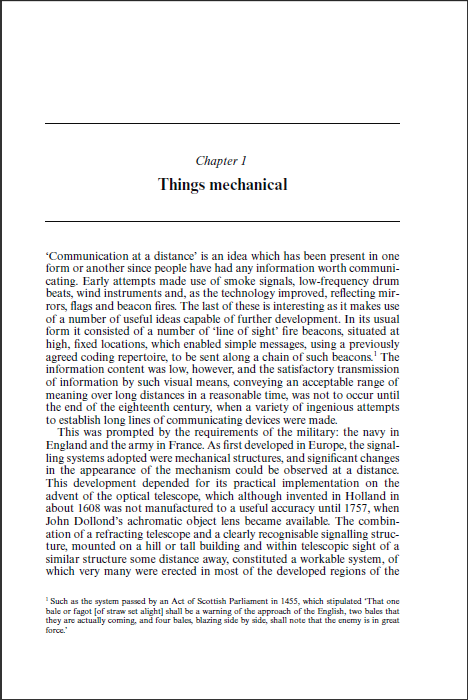
\includegraphics[width=0.6\textwidth]{./chapters/chapter05}
\end{figure}

%\section{General notes on rules}

LaTeX's default rules would normally give problems. Best is to use TeX's primitives to built them.

%\index{rules!example color}
%\begin{texexample}{}{}
%\makeatletter
%\hrule width 5cm \kern2.6\p@
%AAAAAAAAAAAAAAAAAAAAA
%\vskip2.6pt\hrule width 5cm
%\medskip
%
%Problem with LaTeX rules.
%
%\rule{5cm}{0.4pt}\par
%AAAAAAAAAAAAAAAAAAAAA\par%
%\rule[6.5pt]{5cm}{0.4pt}
%
%\def\rule{\@ifnextchar[\@rule{\@rule[\z@]}}
%\def\@rule[#1]#2#3{%
% \leavevmode
% \hbox{%
% \setlength\@tempdima{#1}%
% \setlength\@tempdimb{#2}%
% \setlength\@tempdimc{#3}%
% \advance\@tempdimc\@tempdima%
% \vrule\@width\@tempdimb\@height\@tempdimc\@depth-\@tempdima}}
%
%\def\thickrule{\leavevmode \leaders \hrule height 3pt \hfill \kern \z@}
%
%{\color{teal}\hrule width 10.5cm height3pt \kern2.6\p@
%    {{\color{black!80}\HUGE CHAPTER TITLE}}\vskip3pt
%\hrule width 10.5cm height3pt}
%\makeatother
%\end{texexample}

% <<<<<<< HEAD
%%%%%%%%%%%%%%%%%%%%%%%%%%%%%%%%%%%%%%%%%%%
%%%%%%  STYLE 06
%%%%%%%%%%%%%%%%%%%%%%%%%%%%%%%%%%%%%%%%%%%

\cxset{style06/.style={
 name={Chapter},
 numbering=arabic,
 number font-size=\Huge,
 number font-family=\calligra,
 number font-weight=\calligra,
 number color=\color{black!90},
 number before=\kern-2.5pt,
 number dot=,
 number after=,
 number position=rightname,
 chapter font-family=\rmfamily,
 chapter font-weight=\calligra,
 chapter font-size=\LARGE\calligra,
 chapter before={\vspace*{20pt}\par\hfill},
 chapter after={\hfill\hfill\par},
 chapter color={black!90},
 title beforeskip={\vspace*{50pt}},
 title afterskip={\vspace{3.5pt}\par},
 title before={\hfill},
 title after={\hfill\hfill},
 title font-family=\rmfamily,
 title font-color=\color{black!90},
 title font-weight=\normalfont,
 title font-size=\LARGE,
 title spaceout=soul,
}}

\cxset{style06}

\chapter{INTRODUCTION TO STYLE SIX}
\renewcommand{\DefaultLhang}{0.1}
\renewcommand{\LettrineFontHook}{\calligra}
\setlength{\DefaultFindent}{9.5pt}
\setlength{\DefaultNindent}{0pt}

\lettrine{\textcolor{orange}{T}}{}he calligraphic font for this design make it stand out, although you may need to experiment to get the right font (I have used calligra). I am sure the specification can be optimized a bit, however so far it works. I also opted to space out the title. I had to experiment a bit to get the Lettrine settings.
\medskip
\begin{figure}[ht]
\centering
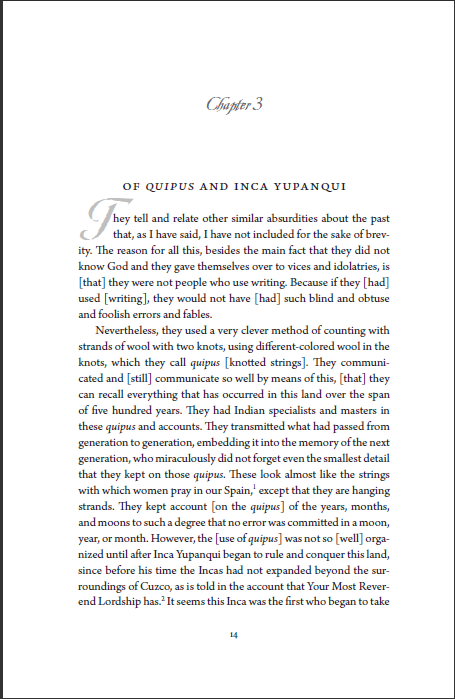
\includegraphics[width=0.6\textwidth]{./chapters/chapter06}
\end{figure}

The number has been kerned using:

\begin{lstlisting}
 number before=\kern-4.5pt,
\end{lstlisting}

This template has a lot of potential and I will come back to it and add more key hooks for lettrine settings per letter and font management. They can also come alive with a gold color.

=======
%%%%%%%%%%%%%%%%%%%%%%%%%%%%%%%%%%%%%%%%%%%
%%%%%%  STYLE 06
%%%%%%%%%%%%%%%%%%%%%%%%%%%%%%%%%%%%%%%%%%%

\cxset{style06/.style={
 name={Chapter},
 numbering=arabic,
 number font-size=\Huge,
 number font-family=\calligra,
 number font-weight=\calligra,
 number color=\color{black!90},
 number before=\kern-2.5pt,
 number dot=,
 number after=,
 number position=rightname,
 chapter font-family=\rmfamily,
 chapter font-weight=\calligra,
 chapter font-size=\LARGE\calligra,
 chapter before={\vspace*{20pt}\par\hfill},
 chapter after={\hfill\hfill\par},
 chapter color={black!90},
 title beforeskip={\vspace*{50pt}},
 title afterskip={\vspace{3.5pt}\par},
 title before={\hfill},
 title after={\hfill\hfill},
 title font-family=\rmfamily,
 title font-color=\color{black!90},
 title font-weight=\normalfont,
 title font-size=\LARGE,
 title spaceout=soul,
}}

\cxset{style06}

\chapter{INTRODUCTION TO STYLE SIX}
\renewcommand{\DefaultLhang}{0.1}
\renewcommand{\LettrineFontHook}{\calligra}
\setlength{\DefaultFindent}{9.5pt}
\setlength{\DefaultNindent}{0pt}

\lettrine{\textcolor{orange}{T}}{}he calligraphic font for this design make it stand out, although you may need to experiment to get the right font (I have used calligra). I am sure the specification can be optimized a bit, however so far it works. I also opted to space out the title. I had to experiment a bit to get the Lettrine settings.
\medskip
\begin{figure}[ht]
\centering
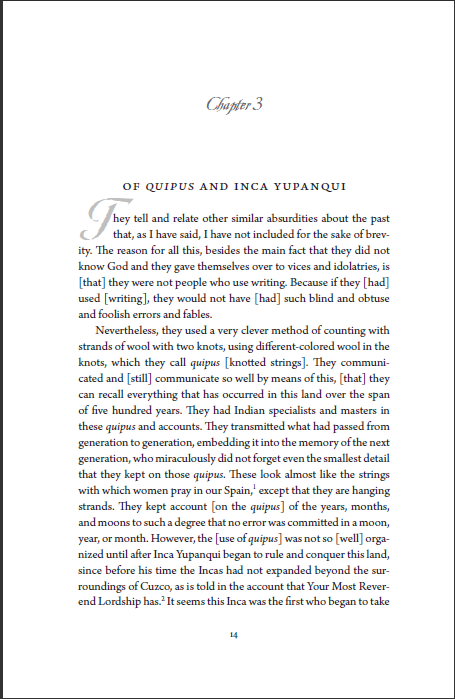
\includegraphics[width=0.6\textwidth]{./chapters/chapter06}
\end{figure}

The number has been kerned using:

\begin{lstlisting}
 number before=\kern-4.5pt,
\end{lstlisting}

This template has a lot of potential and I will come back to it and add more key hooks for lettrine settings per letter and font management. They can also come alive with a gold color.

>>>>>>> merged

% 
\newgeometry{top=2cm,bottom=2cm,left=3cm,right=3cm}

\setdefaults

\cxset{style07/.style={
 name={},
 chapter toc=true,
 numbering=arabic,
 number font-size=HUGE,
 number font-family=sffamily,
 number font-weight=bfseries,
 number before=,
 number dot=,
 number color= gray,
 number after=\par,
 number position=leftname,
 chapter font-family=\sffamily,
 chapter font-weight=\normalfont,
 chapter font-size=\Large,
 chapter before={\hfill\hfill\hfill\par},
 chapter after={\vspace*{20pt}},
 chapter color= black!90,
 title beforeskip={\vspace*{30pt}},
 title afterskip={\vspace*{50pt}\par},
 title before={},
 title after={\par\rule[17pt]{\textwidth}{0.4pt}},
 title font-family=\sffamily,
 title font-weight=\bfseries,
 title font-size=\LARGE,
 title font-shape=normal,
 title font-color=black!90,
 title spaceout=none,
}}

\cxset{style07}
\chapter{Introduction to Style Seven}

\parindent0pt
\lipsum[1]
\medskip
\begin{figure}[ht]
\centering
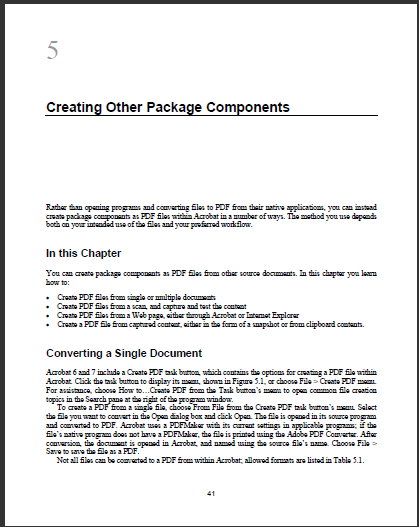
\includegraphics[width=0.6\textwidth]{./chapters/chapter07.png}
\end{figure}
\lipsum[1]

% \clearpage

\setdefaults

\makeatletter
\cxset{style08/.style={
 name={},
 chapter toc=true,
 numbering=arabic,
 number font-size=\LARGE,
 number font-family=\sffamily,
 number font-weight=\bfseries,
 number color= black!90,
 number before=,
 number dot=,
 number after=,
 number position=rightname,
 chapter font-family=sffamily,
 chapter font-weight=normalfont,
 chapter spaceout=none,
 chapter font-size=Large,
 chapter before=,
 chapter after=,
 chapter color={black!90},
 chapter float=right,
 chapter display=block,
 chapter border-style=none,
 chapter border-width=0pt,
 number spaceout=none,
 number display=block,
 number float=right,
 chapter title width=0.6\textwidth,
 title beforeskip=,
 title afterskip=,
 title before=,
 title after={},
 title font-family=sffamily,
 title font-color=black!90,
 title font-weight=bfseries,
 title font-size=LARGE,
 title display=block,
 chapter title align=right,
 author block=true,
 author block format=\par\addvspace{12pt}\normalfont\large\raggedleft,
 author names=Yiannis Lazarides\par Larnaka,
 section number after=,
 section numbering = arabic,
 section numbering prefix=,
 section numbering custom = \@arabic\c@section.\space,
 section color=black,
 section numbering suffix=,
 header style=empty}}
 
 % humanized name of the style, with a non human connotation!
 %
 \cxset{humanoid/.style={style08}}
\makeatother

\cxset{section color=sweet,
          section font-shape=sffamily}


\cxset{style08}
% set the counter needs this to be modified to be based on a key value interface
\cxset{figure numbering/.is choice,
          figure numbering/within/.code=\counterwithin{figure}{chapter},
          figure numbering/without/.code=\counterwithout{figure}{chapter}}
\cxset{table numbering/.is choice,
          table numbering/within/.code=\counterwithin{table}{chapter},
          table numbering/without/.code=\counterwithout{table}{chapter}}          
%\counterwithout{figure}{chapter}

\cxset{figure numbering=without,
          table numbering=without}

\captionsetup[figure]{format = plain,    
                                 width=.67\textwidth,
                                 justification=justified,
                                 singlelinecheck=false,
                                 name=Fig.,
                                 labelsep=period,
                                 oneside,
                                 margin=0pt,
                                 font={normalsize,up}
                                 }
\captionsetup[table]{format = plain,    
                                 justification=justified,
                                 singlelinecheck=false,
                                 labelsep=period,
                                 oneside,
                                 margin=0pt,
                                 labelfont={up,it,normalfont}
                                 }
\chapter[Style 08]{Introduction to Book Style Eight Some Old Fashioned Stops}
\label{st:eight}
\section{Introduction}

This style is suited for Academic publishing, where editors are still a bit old fashioned and require that stops are placed after section numbers, but they do not require that the first line of paragraphs are indented. Any way the good folks that published this book, knew their Affective Computing well and amongst belly dancing  robots and smiling and angry faces, typography can take second place.\footnote{Jimmy Or (\textit{editor}). Affective Computing
Focus on Emotion Expression,
Synthesis and Recognition, May 2008.
}

\example 
\medskip
\begin{figure}[ht]
\centering
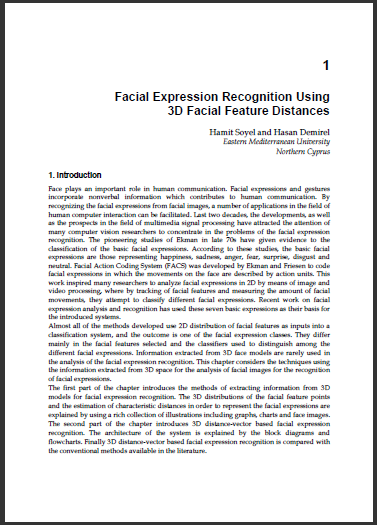
\includegraphics[width=0.5\textwidth]{./chapters/chapter08.png}
\caption{The opening page of a chapter in \textit{Affecting Computing}.}
\end{figure}

\solution To add the dot after the number can be done either using the key
\begin{verbatim}
\cxset{section numbering custom = \@arabic\c@section.,}
\end{verbatim}
or by using the pre-built key
\begin{verbatim}
\cxset{section number after=.}
\end{verbatim}

The author block including the institution are added as part of the chapter head styling command.

\example The subject of having articles together in a publication such as Proceedings and Journals is a recurring theme in many Academic fields. One of course if it is possible would have liked to use a standard Journal class and automatically produce this type of publication. There are a number of such classes at \href{http://ctan.org/tex-archive/macros/latex/required/amslatex/amscls/doc/instr-l.pdf}{ctan}

\solution If you are the editor with the task of assembling all these different articles consider using the \pkgname{confproc}. The package by Vincent Verfaille assembles the proceedings from the pdfs, using the 
\pkgname{pdfpages}, which is another great way to achieve this. A simpler way is to develop a specific style for
your Conference and let the participants use it while writing their papers. Only caveat they need to import the
body of the paper with \string\input\meta{article name}. As the \pkgname{phd} comes pre-packaged with
numerous packages the chance of someone using a package that the editor or the system needs to use it
is minimized. Indexing, bibliographies and the like might need to be taken care of and this is discussed in the relevant chapters. There are many options and peculiarities that might not be covered by the phd package so my suggestion is to try it on a few older papers first.

\example  Style-08 has to set the caption style to include for a period after the label number as shown in the Fig.~\ref{fig:eight02}. This can be achieved through key settings or a package.
\begin{figure}[ht]
\centering
\includegraphics[width=\textwidth]{./images/affective-computing.jpg}
\caption{Figures are centered, with the caption flush left and the \textit{Figure} label abbreviated to Fig. (with a stop). The section number also has the dot and follows the style of the sections.}
\label{fig:eight02}
\end{figure}

The figures numbers are reset at every chapter. Normally authors use the \pkgname{chngctr} to achieve such changes, which involves two modifications. Redefining whether or not the figure counter will be reset whenever the chapter/section counter is incremented; Redefining the "appearance" of the figure counter (\string\thefigure), i.e., removing (or adding) the chapter/section prefix.


The standard solution – which deals with modifications 1 and 2 mentioned above – is to use the \string\counterwithout and \string\counterwithin macros of the \texttt{chngcntr package}.\footnote{\protect\url{http://tex.stackexchange.com/questions/28333/continuous-v-per-chapter-section-numbering-of-figures-tables-and-other-docume}} 


\section{Tables}

The Tables follow the style for figures as far as captioning. They are all framed and although there is a genuine distain in the \latexe community for this type of style, I must admit that they are blending well with the style of this book. Another typographical tradition that has been broken in this book is that the table captions are placed below the table and not above.

\example
\begin{figure}[ht]
\centering
\includegraphics[width=\textwidth]{./images/affective-computing-tables.jpg}
\caption{Figures are centered, with the caption flush left and the \textit{Figure} label abbreviated to Fig. (with a stop). The section number also has the dot and follows the style of the sections.}
\label{fig:eight02}
\end{figure}


\begin{verbatim}
\cxset{table numbering=without}
\end{verbatim}

\setlength\extrarowheight{5pt}

\bgroup
\begin{table}[h]
\begin{tabularx}{\textwidth}{|c|c|c|X|}
\hline
Affective Movement & Mean & Standard Deviation &\RaggedRight Standard Error of the Mean\\
\hline
confident & (0.150,0.100,0.150) & (0.362,0.304,0.362)&(0.57,0.48,0.57)\\
\hline
\end{tabularx}
\caption{The table style of the book, with the caption below. You may need to increase the cell lengths.}
\end{table}
\egroup

The cell heights of the table have been increaded by 5pt, using,
\begin{verbatim}
\setlength\extrarowheight{5pt}
\end{verbatim}

\section{Front Matter}

The Front Matter includes a Title Page, Table of Contents and a Preface. Nothing special or exciting here with the exception of the Table of Contents which is a bit on the difficult side. 

\begin{figure}[ht]
\centering
\includegraphics[width=\textwidth]{./images/affecting-computing-contents.jpg}
\caption{Figures are centered, with the caption flush left and the \textit{Figure} label abbreviated to Fig. (with a stop). The section number also has the dot and follows the style of the sections.}
\label{fig:eight02}
\end{figure}

\section{Back Matter}



For the handling of the References there are numerous options and these are discussed under the Bibliography and References chapter.\footnote{\protect\url{http://tex.stackexchange.com/questions/87991/putting-bibliographies-at-the-end-of-each-chapter}} The referencing styles within paragraphs of text are author year in square brackets. I leave this to you.

\begin{figure}[ht]
\centering
\includegraphics[width=\textwidth]{./images/affective-computing-references.jpg}
\caption{Figures are centered, with the caption flush left and the \textit{Figure} label abbreviated to Fig. (with a stop). The section number also has the dot and follows the style of the sections.}
\label{fig:eight02}
\end{figure}

\parindent1em

There are no book divisions, such as an Index at the back of the book, but each chapter has its own references section, styled as a section. The occassional single Appendix appears at the end of a chapter, styled after sections and with no numbering marks.

\section{Concluding Remarks}

This template has a unique character and in my opinion deserves a bit better. Styling for algorithms, computer code additional floating sections and an index is not provided in the template and is left open for the user. It works well with the book class and with the KOMA classes. I have also given it an alias \emph{humanoid}\footnote{From one of the chapters in the book discussing the development of humanoids that can express emotions. The scientific field of human emotions and its applications both on the web as well as robotics is a vast topic. I did waste a lot of time reading the book rather than developing the style. } A minimal to use the template is shown below:

\section{Front Matter}
\begin{figure}[ht]
\centering
\includegraphics[width=\textwidth]{./images/facial-expression-1.jpg}
\caption{Figures are centered, with the caption flush left and the \textit{Figure} label abbreviated to Fig. (with a stop). The section number also has the dot and follows the style of the sections.}
\label{fig:eight02}
\end{figure}


\begin{verbatim}
\documentclass{book}
\usepackage{phd}
\cxset{humanoid}
\begin{document}
... contents
\end{document}
\end{verbatim}

If you do restyle it, please let me know with samples of the work.

\begin{key}{/phd/section align=center}{initial none}

\end{key}




% \cxset{author block=false}
\clearpage
\cxset{
 chapter name=none,
 numbering=arabic,
 number font-size=LARGE,
 number font-family=sffamily,
 number font-weight=mdseries,
 number before=,
 number dot=,
 number display=block,
 number float=left,
 number after={\vrule width2cm height0.4pt depth0pt\relax},
 number position=rightname,
 chapter font-family=sffamily,
 chapter font-weight=normalfont,
 chapter font-size=Large,
 chapter before={\vspace*{10pt}\par},
 chapter after={},
 chapter color={black!90},
 number color= black!90,
 title beforeskip=,
%title afterskip={\vspace*{50pt}\par},
 title margin bottom=40pt,
 title before=,
 title after=,
 title font-family=sffamily,
 title font-color= black,
 title font-weight=normalfont,
 title font-size=LARGE,
 chapter title align=none,
chapter title text-align=left,
chapter title width=\textwidth,
 title margin top=0pt,
 section numbering=none,
 section font-weight=normalfont,
 section indent=0pt,
 section align=centering,
 }
 \renewsection
\chapter{Preparing for Trial}

Template number nine, is from a book about a the Rivonia Trial. The template is easy to set up and is has a simple but effective design, which I think is very appropriate for a journalistic type of book. 
\medskip
\begin{figure}[ht]
\centering
\hspace*{-.1\textwidth}{\color{thegray}\fbox{\includegraphics[width=1.2\textwidth]{mandela-01}}}
\end{figure}

When South Africa's apartheid government charged Nelson Mandela with planning its overthrow in 1963, most observers feared that he would be sentenced to death. But the support he and his fellow activists in the African National Congress received during his trial not only saved his life, but also enabled him to save his country. In Saving Nelson Mandela, South African law expert Kenneth S. Broun recreates the trial--called the ``Rivonia" Trial after the Johannesburg suburb where police seized Mandela. Based upon interviews with many of the case's primary figures and portions of the trial transcript, Broun situates readers inside the courtroom at the imposing Palace of Justice in Pretoria. Here, the trial unfolds through a dramatic narrative that captures the courage of the accused and their defense team, as well as the personal prejudices that colored the entire trial. The Rivonia trial had no jury and only a superficial aura of due process, combined with heavy security that symbolized the apartheid government's system of repression. 

Broun shows how outstanding advocacy, combined with widespread public support, in fact backfired on apartheid leaders, who sealed their own fate. Despite his 27-year incarceration, Mandela's ultimate release helped move his country from the racial tyranny of apartheid toward democracy. As documented in this inspirational book, the Rivonia trial was a critical milestone that helped chart the end of Apartheid and the future of a new South Africa.

``Kenneth Broun does justice indeed to one of the most celebrated political trials of the 20th century...the result is not only a gripping story but a work of profound scholarship, sensitivity, and empathy." --Mark Gevisser, author of A Legacy of Liberation 

``Part history, part sociology, part engrossing legal drama, this important book recounts a seminal moment in South Africa's history." --Penelope Andrews, City University of New York School of Law

Many things are going wrong in South Africa, but it would have been worse if it was not for Mandela.  

To use the template simply load the \pkgname{phd} package and |style09| or |rivonia|. Adjust spacing fonts and geometry to your liking:

\begin{verbatim}
\documentclass{book}
\usepackage{phd}
\phdusetemplate{style09}
\cxset{chapter opening=anywhere}
\begin{document}
\chapter{Arrests and Escapes}
\end{document}
\end{verbatim}

\cxset{chapter opening=anywhere}

\chapter{Arrests and Escapes}

\lorem

\section{Adjusting the Rule}

You might want to fiddle with the rule settings, as well as the section settings. I prefer the sections centered and not numbered.

\thispagestyle{headings}









% <<<<<<< HEAD
%%%%%%%%%%%%%%%%%%%%%%%%%%%%%%%%%%%%%%%%%%%
%%%%%%  STYLE 10
%%%%%%%%%%%%%%%%%%%%%%%%%%%%%%%%%%%%%%%%%%%

\cxset{
 name=CHAPTER,
 numbering=WORDS,
 number font-size=\huge,
 number font-family=\sffamily,
 number font-weight=\bfseries,
 number before=,
 number dot=,
 number after=\hspace{1em},
 number position=rightname,
 chapter font-family=\sffamily,
 chapter font-weight=\bfseries,
 chapter font-size=\huge,
 chapter before={\vspace*{0.4\textheight}\hfill},
 chapter after={\hfill\hfill\vskip0pt\thinrule\par},
 chapter color={black!90},
 number color=\color{black!90},
 title beforeskip={\vspace*{30pt}},
 title afterskip={\vspace*{30pt}\par},
 title before={\hfill},
 title after={\hfill\hfill},
 title font-family=\sffamily,
 title font-color=\color{black!90},
 title font-weight=\bfseries,
 title font-size=\huge,
 section font-size=\LARGE,
 section font-weight=\normalfont,
 section font-family=\sffamily,
 section align=,
 section numbering=none,
 section indent=-1em,
 section align=\centering,
 section beforeskip=20pt,
 section afterskip=10pt,
 section spaceout=soul,
 section font-shape=,
}

 %set the sectioning commands


\renewsection

\chapter{INTRODUCTION TO STYLE TEN}

\section{Basic Description:}
This chapter style has the unique characteristic that the chapter number is spelled out, rather than being in arabic numerals. The setting for this is the option \lstinline{numeric=WORDS}. Use either a capital for uppercase or \lstinline{numeric=words} for lowercase number labels.

\medskip
\begin{figure}[ht]
\centering
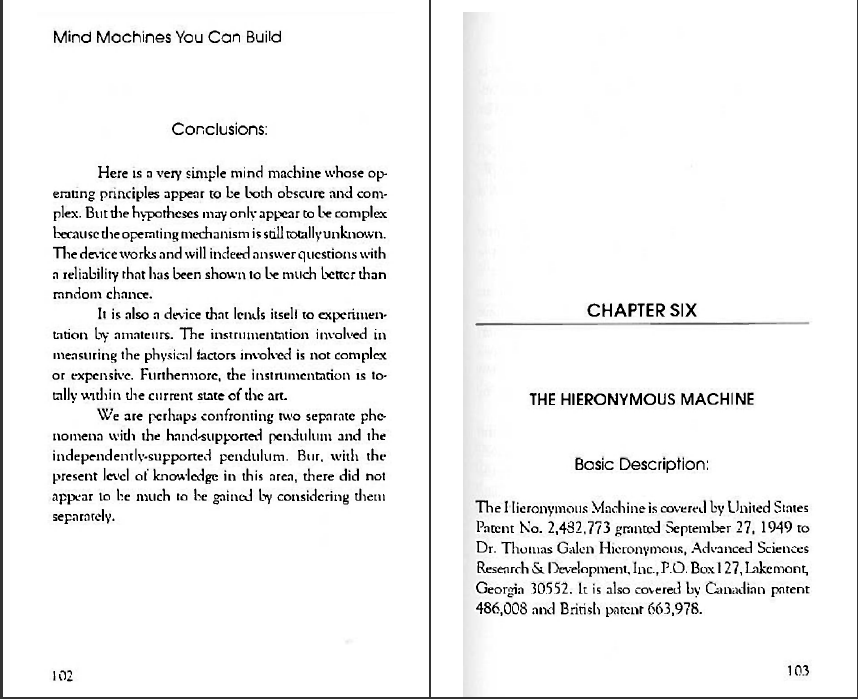
\includegraphics[width=0.6\textwidth]{./chapters/chapter10}
\end{figure}

\lipsum[1]
=======
%%%%%%%%%%%%%%%%%%%%%%%%%%%%%%%%%%%%%%%%%%%
%%%%%%  STYLE 10
%%%%%%%%%%%%%%%%%%%%%%%%%%%%%%%%%%%%%%%%%%%

\cxset{
 name=CHAPTER,
 numbering=WORDS,
 number font-size=\huge,
 number font-family=\sffamily,
 number font-weight=\bfseries,
 number before=,
 number dot=,
 number after=\hspace{1em},
 number position=rightname,
 chapter font-family=\sffamily,
 chapter font-weight=\bfseries,
 chapter font-size=\huge,
 chapter before={\vspace*{0.4\textheight}\hfill},
 chapter after={\hfill\hfill\vskip0pt\thinrule\par},
 chapter color={black!90},
 number color=\color{black!90},
 title beforeskip={\vspace*{30pt}},
 title afterskip={\vspace*{30pt}\par},
 title before={\hfill},
 title after={\hfill\hfill},
 title font-family=\sffamily,
 title font-color=\color{black!90},
 title font-weight=\bfseries,
 title font-size=\huge,
 section font-size=\LARGE,
 section font-weight=\normalfont,
 section font-family=\sffamily,
 section align=,
 section numbering=none,
 section indent=-1em,
 section align=\centering,
 section beforeskip=20pt,
 section afterskip=10pt,
 section spaceout=soul,
 section font-shape=,
}

 %set the sectioning commands


\renewsection

\chapter{INTRODUCTION TO STYLE TEN}

\section{Basic Description:}
This chapter style has the unique characteristic that the chapter number is spelled out, rather than being in arabic numerals. The setting for this is the option \lstinline{numeric=WORDS}. Use either a capital for uppercase or \lstinline{numeric=words} for lowercase number labels.

\medskip
\begin{figure}[ht]
\centering
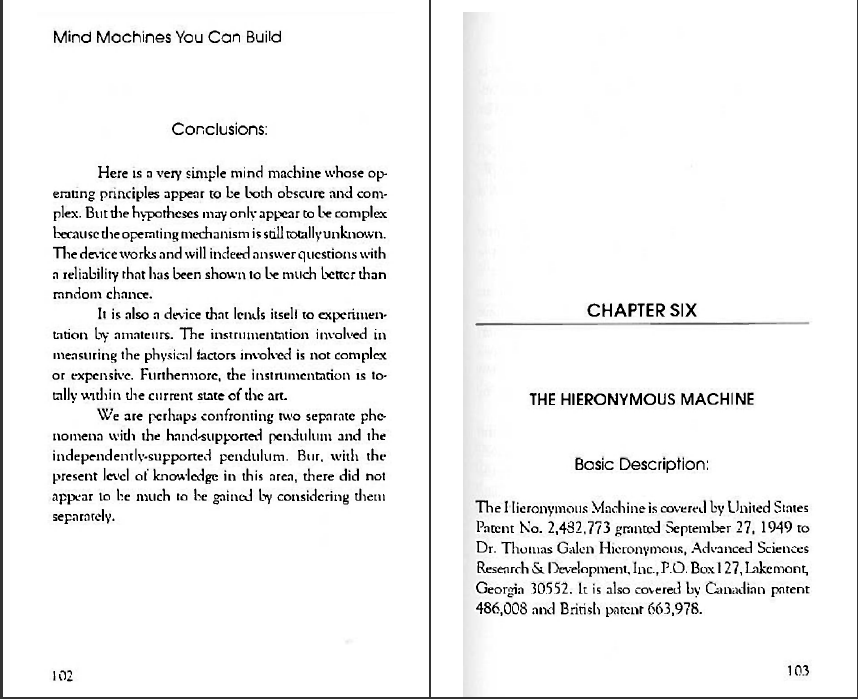
\includegraphics[width=0.6\textwidth]{./chapters/chapter10}
\end{figure}

\lipsum[1]
>>>>>>> merged

% \cxset{style11/.style={
 chapter opening=any,
 name=Chapter,
 numbering=arabic,
 number font-size=LARGE,
 number font-family=rmfamily,
 number font-weight=bfseries,
 number before=,
 number dot=,
 number after=,
 number before=\kern0.5em,
 number display=inline,
 number float=center,
 chapter display=block,
 chapter float=center,
 chapter font-family=rmfamily,
 chapter font-weight=bfseries,
 chapter font-size=LARGE,
 chapter before=,
 chapter after=,
 chapter color=black!90,
 chapter spaceout=none,
 chapter border-width=0pt,
 chapter border-style=none,
 number color=black!90,
 title beforeskip=,
 title afterskip=,
 title before=,
 title after=,
 title font-family=rmfamily,
 title font-color=black!90,
 title font-weight=bfseries,
 title font-size=LARGE,
 chapter title width=\textwidth,
 chapter title align=centering,
 section afterindent=true,
 section align=left,
 section numbering=arabic,
 section numbering prefix=\thechapter.,
 section numbering suffix=\space,
 section indent=0pt,
 section font-family=rmfamily,
 }}
\renewsection\renewsubsection

\cxset{style11}
\chapter{\textit{Elements} II and Babylonian Metric Algebra, Introduction to Style Eleven}

The origins of Greek Mathematics, according to the Greeks is Egypt and according to J\"oran Friberg is Babylonia. This template is based on Friberg's book \emph{Amazing Traces of a Babylonian Origin in Greek Mathematics}. The book was published by World Scientific in 2007. The book size is $5.97\times8.88$ inches and uses a variety of fonts, with the main document font in Times. 

\medskip
\begin{figure}[ht]
\centering
\fbox{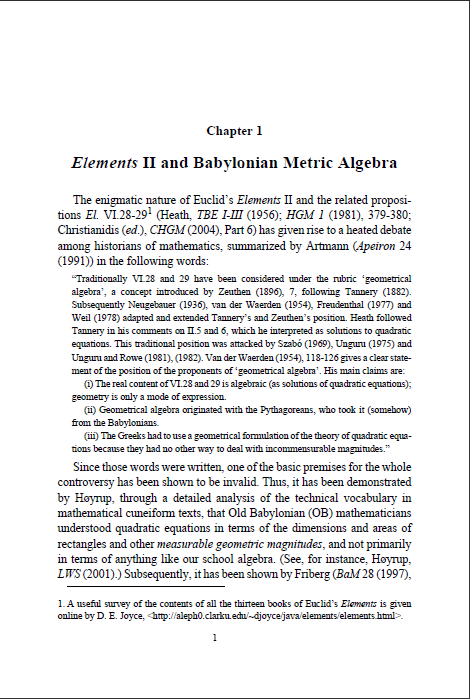
\includegraphics[width=0.65\textwidth]{./chapters/chapter11.png}}
\end{figure}
\lipsum[1]

\section{Indentation}

The book follows swedish traditional typography with the paragraphs following subheadings indented. This is achieved in the template using:

\begin{verbatim}
\cxset{section afterindent=true}
\end{verbatim}

\section{Images}
\indent Images and their captions follow a \latexe style and I am sure the book must have been styled using a \latexe xml clone as the book's pdf was produced with iText\footnote{\url{http://itextpdf.com/}}.

\begin{figure}[ht]
\centering
\includegraphics[width=0.8\textwidth]{greekmaths}
\caption{Extract from the \textit{Amazing Traces of Babylonian Influence in Greek Mathematics.} Note the styling of the caption.}
\end{figure}

\testsections

% reset for following chapters
\cxset{section afterindent=false}


% \parindent0pt
\makeatletter
\cxset{style12/.style={%
 chapter name=,
 chapter toc=true,
 chapter numbering=arabic,
 number font-size=HUGE,
 number font-family=rmfamily,
 number font-weight=bfseries,
 number before=,
 number dot=,
 number color= gray,
 number after=,
 number position=rightname,
 number float=left,
 number display=block,
 chapter font-family=sffamily,
 chapter font-weight=normalfont,
 chapter font-size=huge,
 chapter before=,
 chapter after=,
 chapter color={black!90},
 title beforeskip={\vspace*{0pt}},
 title afterskip={\vspace*{50pt}\par},
 title before=,
 title after={\par\vspace{20pt}\rule{\textwidth}{4pt}},
 title font-family=sffamily,
 title font-color=black!90,
 title font-weight=bfseries,
 title font-size=Huge,
 title font-shape=normal,
 title spaceout=none,
 chapter title width=.8\textwidth,
 chapter title align=left,
 chapter title text-align =left,
}}
\makeatother

\cxset{style12}
\chapter{Why Have They Become Mainstream so Quickly? }
\label{ch:style12}
This is a variation of Style 7, with only the lettering and the rule are thicker. In my opinion it looks better with a bit of color, so I have used a purple color with a gray.

\medskip
\begin{figure}[ht]
\centering
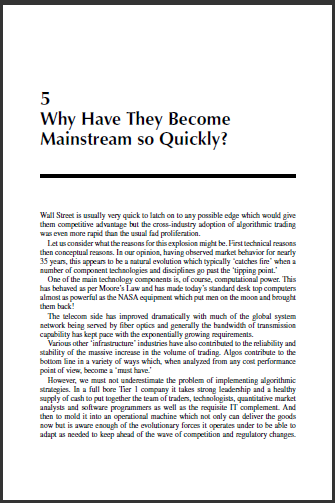
\includegraphics[width=0.35\textwidth]{./chapters/chapter12.png}
\caption{Style 12 sample from the book.}
\end{figure}
\lipsum[1]


% \cxset{%
 chapter opening=any,
 name=Chapter,
 numbering=arabic,
 number font-size=HHUGE,
 number font-family=rmfamily,
 number font-weight=bfseries,
 number before=,
 number dot=,
 number after=,
 number position= rightname,
 number display=block,
 number float=right,
 chapter display=block,
 chapter float=right,
 chapter font-family=\sffamily,
 chapter font-size=\Large,
 chapter before={\offinterlineskip\hbox{\vrule height2pt width\textwidth}\vskip3.5pt}\hfill,
 chapter after=\vskip3.5pt,
 chapter color=black!90,
 number color=black!90,
 chapter title width={0.5\textwidth},
 title margin-left=0pt,
 chapter title align=right,
 chapter title text-align=raggedleft,
 chapter margin top=0pt,
 chapter margin-left=0pt,
 title margin top=0pt,
 title margin bottom=10pt,
 title before={},
 title after={},
 title font-family=sffamily,
 title font-color=black!90,
 title font-weight=bfseries,
 title font-size=LARGE,
 section numbering prefix=\thechapter.,
 section color=black,
 subsection color=black}
 
\chapter{Review of Basic Fluid Mechanics Concepts}
\thispagestyle{headings}

This book is $5.51\times9.06$ inches and was produced according with the soft copy I have with Acrobat Distiller 5.0 (Windows). It uses a variety of fonts Arial, Century Schoolbook and Helvetica, Times Roman, MathematicalPi-One.
\medskip
\begin{figure}[ht]
\centering
\fbox{%
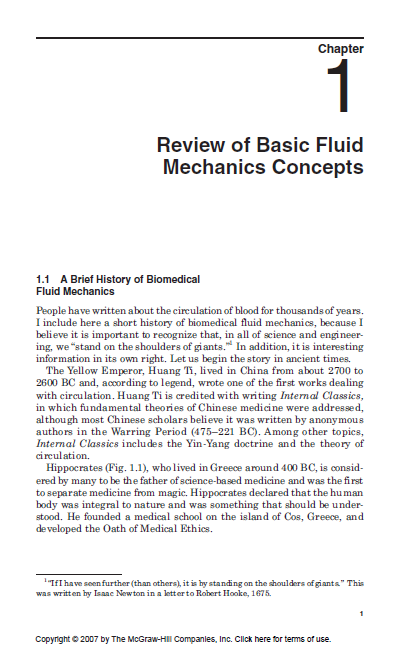
\includegraphics[width=0.45\textwidth]{./chapters/chapter14}
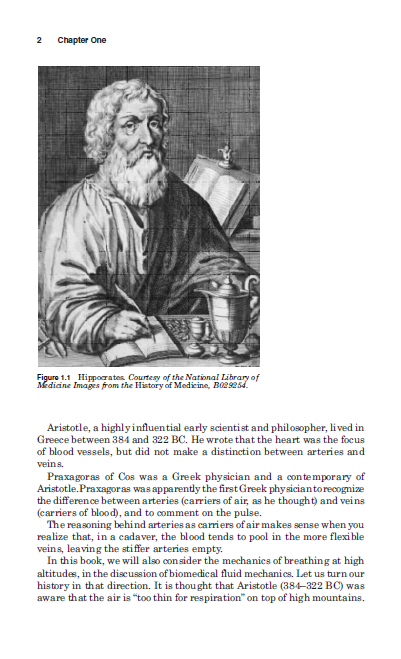
\includegraphics[width=0.45\textwidth]{./chapters/chapter14a.png}}
\end{figure}
\lipsum[2]

\section{Images}

\begin{figure}[ht]
\centering
\includegraphics[width=0.8\textwidth]{biofluids}
\end{figure}
\lipsum[2]

\lipsum[1]
\section{Examples}
Both full page ad well as block examples exist, these are all in boxes and they are numbered either with subsection counters in a fashion that is continuous from the text. 
\begin{figure}[ht]
\centering
\includegraphics[width=0.8\textwidth]{biofluids-1}
\end{figure}
\lipsum[2-4]

\begin{figure}[!b]
\begin{scriptexample}{This is a test}{}
\subsection{Clinical feature: polycythemia}

Polycythemia refers to a condition in which there is an increase in hemoglobin
above 17.5 g/dL in adult males or above 15.5 g/dL in females
(Hoffbrand and Pettit, 1984). There is usually an icrease in the number of
red blood cells above 6 - 1012 $L{^1}$ in males and 5.5 - 1012 $L^{-1}$ in females.
That is, a sufferer from this condition has a much higher blood viscosity due
to this elevated red blood cell count.
\end{scriptexample}
\end{figure}

Our boxes with the \pkgname{tcolorbox} are more than adequate for the job. The color settings can be changed via normal tcolorbox key settings that I have linked to the phd package keys.

The boxes can be also turned into floating boxes and to force them either to be on a full page or at the bottom in order for them to make a better impact in the layout. Key settings for setting the color of the boxes are provided
as well as a special environment.

\begin{verbatim}
\cxset{example box color=thegray}
\end{verbatim}

These example or sideboxes can easily be modified and you may have to provide your own, if you want anything particularly fancy. See the tcolorbox manual for many setting, but please do not use rounded boxes. 
%\end{document}
% %%%%%%%%%%%%%%%%%%%%%%%%%%%%%%%%%%%%%%%%%%%
%%%%%%  STYLE 15
%%%%%%%%%%%%%%%%%%%%%%%%%%%%%%%%%%%%%%%%%%%
\newgeometry{left=2cm,right=7cm, marginparsep=15pt, marginparwidth=4.2cm,top=2cm}
\cxset{
 name={},
 numbering=none,
 number font-size=\LARGE,
 number font-family=\rmfamily,
 number font-weight=\bfseries,
 number before=,
 number dot=,
 number after=,
 number position=rightname,
 chapter font-family=\sffamily,
 chapter font-weight=\normalfont,
 chapter font-size=\Large,
 chapter before={},
 chapter after={},
 chapter color={black!90},
 number color=\color{purple},
 title beforeskip={},
 title afterskip={\vspace*{50pt}\par},
 title before={},
 title after={},
 title font-family=\rmfamily,
 title font-color=\color{black!80},
 title font-weight=\normalfont,
 title font-size=\Huge,
 title font-shape=\itshape,
 chapter opening=any,
 watermark text=SAMPLE PAGE,
 header style=samplepage}


\chapter{Introduction to Style Fifteen}

\parindent1em
\def\thefigure{\arabic{chapter}.\arabic{figure}}
\lorem\par

\marginpar{%
 {\centering
 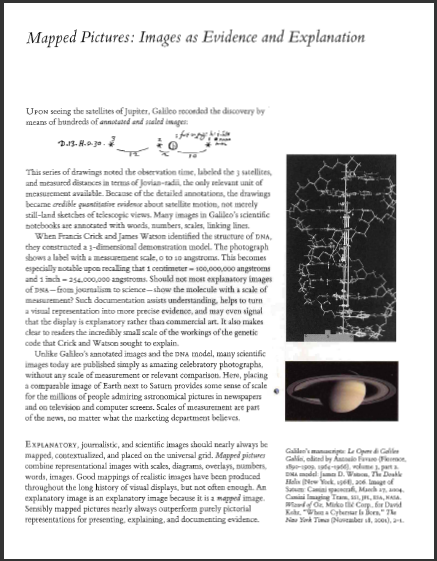
\includegraphics[width=4.2cm]{./chapters/chapter15}\vskip5pt\par}
 {\footnotesize\lorem}
}
\marginpar{%
{\centering
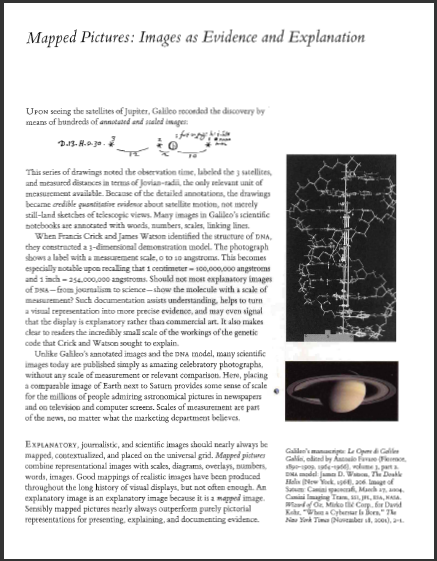
\includegraphics[width=4.2cm]{./chapters/chapter15}\par}
 { \captionof{figure}{\footnotesize\lorem}}
}
This is another marginpar of the same size.

\lorem

\lipsum
\marginpar{%
{\centering
\includegraphics[width=4.2cm]{./chapters/chapter15}\par}
 { \captionof{figure}{\footnotesize\lorem}}
}
%%%% END STYLE %%%%%%%%%%%%%%%%%%%%%%%%%%%%%%%%%

% 
\newgeometry{left=7.5cm,right=2cm, marginparsep=15pt, marginparwidth=4.2cm,top=2cm}
%%%%%%%%%%%%%%%%%%%%%%%%%%%%%%%%%%%%%%%%%%%
%%%%%%  STYLE 16
%%%%%%%%%%%%%%%%%%%%%%%%%%%%%%%%%%%%%%%%%%%


\cxset{style16/.style={
 chapter opening=anywhere,
 name={},
 numbering=arabic,
 number color=\color{thegray},
 number font-size=\HHUGE,
 number font-family=\rmfamily,
 number font-weight=\bfseries,
 number before=\leftskip-4cm\vbox to 0cm\bgroup\vspace*{5cm},
 number after=\egroup\vskip0pt\par,
 number dot=,
 number position=leftname,
 chapter font-family=\sffamily,
 chapter font-weight=\normalfont,
 chapter font-size=\Large,
 chapter before={},
 chapter after={\begin{picture}(0,0)
                          \put(-50pt,\dimexpr-\textheight+\footskip+20pt\relax){\parbox{\marginparwidth}{\textbf{Napoleon}\par\lorem}}%
                        \end{picture}},
 chapter color={black!90},
 title beforeskip={\par\hspace*{4cm}\thinrule\vskip0pt\hspace*{4cm}\vbox\bgroup},
 title afterskip={\vspace*{50pt}\par\egroup},
 title before={},
 title after=,
 title font-color=\color{black!80},
 title font-weight=\normalfont,
 title font-family=\rmfamily,
 title font-shape=\upshape,
 title font-size=\HUGE,
 header style=empty,
 subsection numbering=none,
 subsection color=teal,
 subsection align=\color{teal},
 header style=empty,
 }}

\renewsubsection

%%%% VERSO NAPOLEON %%%%%%%%%%%
% We define a macro to set the page dimensions to full.
% We also require the parindent to be set to 0pt and to restore it afterwards.
\def\fullpageimage{%
       \vspace*{-2.5cm}
        \parindent0pt
       \hspace*{-2cm}\includegraphics[width=\paperwidth]{napoleon}%

}


\cleardoublepage
\fullpageimage

\cxset{style16}
\chapter{Victorian England:\\ Introduction 16}
\label{style16}
This design from a Social Sciences book had to be set into two vboxes and negative skips allowed to line
up the numbers. Once I am totally happy with it, I will add parameter adjustments, as well as a bit of automation of length calculations.
\thispagestyle{empty}

\medskip

\begin{figure}[ht]
\centering
\includegraphics[width=0.35\textwidth]{./chapters/chapter16}
\end{figure}
\lipsum[2]

\cxset{geometry marginparsep/.code=\setlength\marginparsep{#1},
          geometry marginparwidth/.code=\setlength{\marginparwidth}{#1}}

\section{Technical notes}

This design looks simple but takes a bit of effort to achieve it, especially due to the tendency of LaTeX and the TeX engine to make decisions for you. Firstly we cannot reset the page geometry between the image and the chapter, as this will either result in unpredictable behaviour or if you use the \cs{newgeometry} macro, it will for certain leave a blank page in between.

\begin{description}
\item [image sizing] The image is set at \textbf{width=paperwidth}. This can vary depending on the page geometry and the image aspect ratio. In general you may need to ensure that your image has the same aspect ratio as the page to avoid problems with placement and the generation of extra blank pages.
\item [image caption] The image caption is placed using the picture environment, so that it can be typeset absolutely, feel free to use TikZ for the same purpose. We also use Heiko Oberdiek's the \pkg{picture} package to make calculations easier by specifying actual dimensions and not needing to strip the point.
\end{description}

% Best to always restore geometry after you have changed it.

\restoregeometry


% %%%%%%%%%%%%%%%%%%%%%%%%%%%%%%%%%%%%%%%%%%%
%%%%%%  STYLE 17
%%%%%%%%%%%%%%%%%%%%%%%%%%%%%%%%%%%%%%%%%%%
\newgeometry{left=7cm,right=2cm, marginparsep=15pt, marginparwidth=4.2cm,top=2cm,%
reversemarginpar}
\cxset{style17/.style={
 name={},
 numbering=arabic,
 number font-size=\huge,
 number font-family=\sffamily,
 number font-weight=\bfseries,
 number before=,
 number dot=.,
 number color=\color{purple},
 number after=\thinspace,
 number position=rightname,
 chapter font-family=\sffamily,
 chapter font-weight=\bfseries,
 chapter font-size=\LARGE,
 chapter before={\vspace*{20pt}\par\hfill},
 chapter after={},
 chapter color={black!90},
 title beforeskip={},
 title afterskip={\vspace*{70pt}\par},
 title before={},
 title after={},
 title font-family=\sffamily,
 title font-color=\color{purple},
 title font-shape=\upshape,
 title font-weight=\bfseries,
 title font-size=\huge,
 section numbering=none,
 section beforeskip=10pt,
 section afterskip=10pt,
 section font-family=\rmfamily,
 section font-shape=\slshape,
 geometry marginparwidth=4.5cm,
 geometry marginparsep=20pt}}
\cxset{style17}

\chapter{Introduction to Style Seventeen}

I tend to favour this design for books that have a lot of pictures. It brings the design into the margins and leaves plentiful white space in the margins. From a programming point of view the chapter is the opposite of openany. It has to open on an odd number.

\marginpar{%
\vspace*{0.2\textheight}
\includegraphics[width=\marginparwidth]{./chapters/chapter17}\par
{\footnotesize\lorem}
}

\section{Use the margins}

Adjustments to the geometry layout can be carried out temporarily or permanently via the use of keys and
the geometry package. These are probably the less problematic and easier to set geometry settings.

\section{Margin notes}

Marginal notes use the same mechanism as
floats to communicate with the \cs{output} routine. Marginal notes are distinguished from
floats by having a negative placement specification. The command
\cs{marginpar}\oarg{left text}\marg{right text} generates a marginal note in a parbox,
using LTEXT if it's on the left and RTEXT if it's on the right.
(Default is RTEXT = LTEXT.) It uses the following parameters.
\cs{marginparwidth}: Width of marginal notes.
\cs{marginparsep}: Distance between marginal note and text.
the page layout to determine how to move the marginal
note into the margin. E.g.,

\begin{tcolorbox}
\begin{lstlisting}
\@leftmarginskip ==\hskip -\marginparwidth \hskip -\marginparsep .
\end{lstlisting}
\end{tcolorbox}

\cs{marginparpush} Minimum vertical separation between \cs{marginpar}'s
Marginal notes are normally put on the outside of the page
if @mparswitch = true, and on the right if @mparswitch = false.
The command \cs{reversemarginpar} reverses the side where they
are put. \cs{normalmarginpar} undoes \cs{reversemarginpar}.
These commands have no effect for two-column output.
\marginpar{\footnotesize \textsc{\bfseries NOTE:} if two marginal notes appear on the same line of
text, then the second one could appear on the next page, in
a funny position.}
\section{Sample text}
\lipsum[2-4]

\restoregeometry

% \restoregeometry

\cxset{
 name={CHAPTER},
 numbering=arabic,
 number font-size=\Large,
 number font-family=\rmfamily,
 number font-weight=\normalfont,
 number before=\kern0.5em,
 number after=\hfill\hfill\par\vspace*{20pt}\centerline{\decoone}\vspace*{20pt},
 number dot={},
 number position=rightname,
 name=CHAPTER,
 chapter font-family=rmfamily,
 chapter font-weight=mdweight,
 chapter font-size=Large,
 chapter before={\vspace*{20pt}\par\hfill},
 chapter after={},
 chapter color=black!90,
 number color=black!90,
 chapter title align=center,
 chapter title text-align=center,
 title margin-left=0pt,
 title margin bottom=50pt,
 title margin top=30pt,
 title before=,
 title after=,
 title font-family=rmfamily,
 title font-shape=upshape,
 title font-color= black!90,
 title font-weight=\normalfont,
 title font-size=Huge,
 title display=block}

\chapter[Style 18]{Chapter Style Eighteen}

\parindent0pt
This design introduces an ornament. There are a number of packages on ctan that provide ornaments. If you using XeLaTeX it is also possible to use system fonts. The ornament is introduced with the key number after. At this point also we introduced all the vertical skips.
\medskip
\begin{figure}[ht]
\centering
\includegraphics[width=0.45\textwidth]{./chapters/chapter18.png}
\end{figure}

\section{Sections}
\lorem

\subsection{Subsections}
\lorem


\subsubsection{Subsubsections}
\lorem

\parindent3em
\newcommand{\wb}[2]{\fontsize{#1}{#2}\usefont{U}{webo}{xl}{n}}
\newcommand{\showb}[1]{\wb{12}{14}#1}
\newfontfamily{\minion}{MinionPro-Regular.otf}
\def\ornament{{\minion \char"2740}}

\cxset{chapter name=,
          epigraph align=center,
          epigraph text align=center,
          epigraph rule width=0pt,
          title margin top=10pt,
          number font-size=small,
          number after=\hfill\hfill\par\vspace*{5pt}\centerline{\showb{[]}}\vspace*{5pt},
           %number after=\hfill\hfill\par\vspace*{5pt}\centerline{\Large\ornament}\vspace*{5pt},
          }
\chapter{THE IMPRESSIONISTS IN NEW YORK}


\epigraph{\ldots\itshape a pile of unsung treasures \ldots}{}
\minion

\lettrine{O}{n 13 March 1886, Paul Durant-Ruel and his young son Charles were travelling} through the streets of Paris, on their way to Gare Gare Saint-Lazare. In the two decades since Paul had
inherited his father’s business, Paris had been transformed. Haussmann had
realized his dream. The city was only three years away from the
Exposition of 1889 and the erection of the new Eiffel Tower, the symbol
of modern Paris. By 1890, Baron Haussmann would be saying of his newly
created capital of Europe, ‘these days, it’s fashionable to admire old Paris,
which people only know about from books’. Some areas of Paris had
hardly changed: the poor still lived in the shacks of Montmartre or the
shanties of Belleville; there were still cholera, typhoid, deaths in childbirth
and infant mortality. But to the uninitiated, those problems were now
hidden from view. Paris had a new image: the new Republic was
streamlined and stylish, the epitome of healthy living and good taste.
Haussmann’s Paris was architecturally modern, stratified by wealth,
quintessentially urban and, above all, commercially prosperous.

\begin{figure}[ht]
\centering
\fbox{%
\includegraphics[width=0.8\textwidth]{impressionist-lives}}
\caption{Spread from the Book \emph{The Private Lives of the Impressionists} by Sue Rose and published by Harper Collins.}
\end{figure}

The ctan repository has two good packages for ornamental fonts \pkgname{webomints} and \pkgname{fourier-orns}. The one shown in the orgininal publication is from Minion Symbols Pro.

They have been inserted in the template by using the |number after| key and a custom command from the \pkgname{webomints}
\bigskip

\begin{scriptexample}{}{}
\begin{verbatim}
\newcommand{\wb}[2]{\fontsize{#1}{#2}\usefont{U}{webo}{xl}{n}}
\newcommand{\showb}[1]{\wb{12}{14}#1}
\end{verbatim}
\end{scriptexample}


\ornament

\let\oldsection\section
\long\def\section{%
\par\medskip
\addvspace{20pt}
\centerline{{\LARGE *}}%
\addvspace{20pt}}


Cézanne wanted nothing to do with any war. Taking Hortense with him,
he left their garret at 53, rue Notre-Dame-des-Champs, and made for Aix.
Zola, who had recently married, returned to Provence with his wife,
heading from there to Marseilles. Monet, still in Trouville, waited for the
time being to see how events would turn out. Degas, Renoir, Bazille and
Manet, who stayed behind, were all eligible to fight

Cézanne had been working right up to the last minute to meet the 1866
Salon deadline. On the last possible day for submitting, a wheelbarrow
arrived outside the Palais de l’Industrie, pushed and pulled by Cézanne
and Oller, his Cuban friend from Suisse’s. Cézanne rushed to unwrap his
paintings, eager to show them to anyone who wanted to see. But by now
his hopes were not particularly high. When both his paintings were
rejected he was hardly surprised. He headed straight back to Aix,
complaining to Pissarro about the ‘rotten’ family he was being forced to
rejoin, all of them ‘boring beyond measure’. 

\section

Sections are marked with a single asterisk like ornament. This is a common element
in many non-fiction as well as fiction books. Some might have anything from on to three
asterisks. Many books printed in the nineteenth century have very fancy end section ornamentation.
I like the simplicity of the one asterisk.

\let\section\oldsection
\cxset{title display=in-line block}



% \colorlet{toprule}{teal}
\colorlet{theblock}{teal}
\makeatletter
\cxset{rule color/.store in={\rulecolor@cx},
          block color/.store in={\blockcolor@cx}}
\cxset{style20/.style={
 rule color=teal!90,
 block color=teal!90,
 name={},
 numbering = arabic,
 number font-size=\HHUGE,
 number color= white,
 number font-family=\sffamily,
 number font-weight=\bfseries,
 number before={\hbox to 0pt{\vbox to -10pt{\colorbox{\blockcolor@cx}{\rule{0pt}{70pt}\HHUGE \color{\blockcolor@cx}1331}}}\vskip1pt\color{\rulecolor@cx}\rule{\textwidth}{5pt}\par\vskip10pt\relax\hspace{2.5em}},
 number after=\hspace{3em},
 number dot={ },
 number position=leftname,
 chapter font-family=\rmfamily,
 chapter font-weight=\normalfont,
 chapter font-size=\huge,
 chapter before={},
 chapter after={\hskip0pt},
 chapter color=black!90,
 title beforeskip={},
 title afterskip={\vspace*{30pt}\par}, 
 title before={\hskip0.2em},
 title after={\par\vspace{0pt}\color{\rulecolor@cx}\rule{\textwidth}{5pt}},
 title font-family=\sffamily,
 title font-color=black!90,
 title font-weight=\bfseries,
 title font-size=\HUGE,
 chapter title width=.7\textwidth,
 chapter title align=centering,
 section color=teal,
 section font-family=\sffamily,
 section font-weight=\bfseries,
 section font-shape=\upshape,
 section indent=-10pt,
 header style=plain}}
 
 \cxset{style20}
 \chapter{Style 20}

% <<<<<<< HEAD
%%%%%%%%%%%%%%%%%%%%%%%%%%%%%
%%%%%%  STYLE 20a
%%%%%%%%%%%%%%%%%%%%%%%%%%%%%%%%%%%%%%%%%%%
\cxset{rule color/.store in={\rulecolor@cx},
          block color/.store in={\blockcolor@cx}}
\cxset{style20a/.style={
 rule color=teal!90,
 block color=cyan,
 name=chapter,
 numbering = arabic,
 number font-size=\HHUGE,
 number color=\color{white},
 number font-family=\sffamily,
 number font-weight=\bfseries,
 number before={\hbox to 0pt{\vbox to -10pt{\colorbox{\blockcolor@cx}{\rule{0pt}{70pt}\HHUGE \color{\blockcolor@cx}1331}}}\vskip1pt\vskip10pt\relax\hspace{2.5em}},
 number after=\hspace{3em},
 number dot={ },
 number position=rightname,
 chapter font-family=\rmfamily,
 chapter font-weight=\normalfont,
 chapter font-size=\large,
 chapter before={},
 chapter after={\hskip0pt},
 chapter color={black!90},
 title beforeskip={},
 title afterskip={\vspace*{30pt}\par}, % before text
 title before={\hskip0.2em},
 title after={\par\vspace{0pt}\color{\rulecolor@cx}\rule{\textwidth}{5pt}},
 title font-family=\sffamily,
 title font-color=\color{black!90},
 title font-weight=\bfseries,
 title font-size=\HUGE,
 section color=teal,
 section font-family=\sffamily,
 section font-weight=\bfseries,
 section font-shape=\upshape\color{teal},
 section indent=-10pt,
 header style=plain}}
\cxset{style20}
\parindent1em
\chapter{STYLE 20}

\lettrine{\textcolor{teal}{T}}{his} style is probably useful in some corporate environment. The layout has been defined traditionally using boxes and skips and can perhaps be improved tremendously via TikZ. I selected this layout from a book titled \textit{Manufacturing at Warp Speed}, Eli Schragenheim, H. William Dettmer, 2001. The original book's chapter header is not coloured. We will use this example to define color schemes and themes.
\index{color schemes}\index{themes}.
\medskip
\begin{figure}[ht]
\centering
\includegraphics[width=0.7\textwidth]{chapter20}
\end{figure}

\section{Creating themes}
The strategy we use to define themes, especially if based on color changes is to define commands to generate them. This way one could define a number of themes fairly quickly.

\section{Adding templates and themes to a library}
Templates that have a lot of themes can be considered libraries and can be loaded with the package. (See the section on libraries).

\begin{texexample}{}{}
\cxset{chapter opening=anywhere}
% #1 style to add themes
% #2 name of theme
% #3 key value list
\newcommand\maketheme[3][style20]{%
\cxset{#1 #2/.style={#1,#3 }}}
% create some themes
\maketheme[style20]{black}{rule color=black,block color=black,}
\maketheme[style20]{blue}{rule color=theblue,block color=theblue,}
\maketheme[style20]{blue}{rule color=theblue,block color=theblue,}
\maketheme[style20]{orange}{rule color=orange,block color=orange,}
\cxset{style20 black}
\chapter{A Test}
\cxset{style20 blue}
\chapter{A Test}
\cxset{style20 orange}
\chapter{A Test}
\end{texexample}

\begin{texexample}{}{}
\fboxrule0pt\fboxsep0pt
\colorbox{teal}{\fbox{\parbox[b]{3cm}{%
\vbox to 0pt{\hbox to 3cm{\hfill\large\itshape\color{white} Chapter\hfill}}
\vbox{}%
\hbox to 3cm{\hfill \color{white}\sffamily\bfseries\HHUGE39\rule{0pt}{60pt}}
\hbox to 3cm{\rule{0pt}{40pt}}
}}}\hspace{0.5em}
\fbox{\parbox[b]{13cm}{%
\huge\color{teal} Paradoxical functional facilitation\\[-1pt] and recovery in neurological\\[-1pt]
 and psychiatric conditions\par
\medskip
\vspace*{20pt}
\color{black}
\large Dr Yiannis Lazaridegj
}}

\end{texexample}
\newcommand\allbluechapter[2][]{%
\fboxrule0pt\fboxsep0pt%
\hspace*{-1em}\fbox{\colorbox{theblock}{\fbox{\parbox[b]{3cm}{%
\vbox to 0pt{\hbox to 3cm{\hfill\large\itshape\color{white} Chapter\hfill}}
\vbox{}%
\hbox to 3cm{\hfill \color{white}\sffamily\bfseries\HHUGE\thechapter\rule{0pt}{60pt}}
\hbox to 3cm{\rule{0pt}{40pt}}%
}}}\hspace{1.5em}
\fbox{\parbox[b]{10cm}{%
\huge\color{teal} #2\par
\medskip
\vspace*{10pt}
\color{black}
\large \authorblockformat@cx\authorblock@cx
}}}
\vspace{25pt}

\thispagestyle{fancy}
}
\clearpage

\@specialtrue
\cxset{custom=allbluechapter,
         header style=plain, %check why is not working
         chapter opening=any,
         subsection numbering=none,
         subsection color=teal,
         subsection font-weight=\bfseries,
         subsection font-shape=\upshape,
         subsection indent=-10pt,
         author block=true,
         author block format=\bfseries\normalfont\raggedright,
         author names={Dr Yiannis Lazarides, Maria Lazarides and Athena Lazarides}}
\renewsubsection\renewsection
\parindent1em
\chapter[Paradoxical facilitation]{Paradoxical functional facilitation\\ and recovery in neurological\\
 and psychiatric conditions}

\section{Introduction}
\lorem

\section{Author Block Formatting}

Each chapter of the book carries the names of its authors, which is typeset as shown above. The standard available fields for author blocks are programmed in the special template. The full settings are shown in Example .
\medskip

\noindent\begin{tcolorbox}
\begin{lstlisting}
\@specialtrue
\cxset{custom=allbluechapter,
         header style=plain, %check why is not working
         chapter opening=any,
         author block=true,
         author block format=\bfseries\normalfont\raggedright,
         author names=Dr Yiannis Lazarides, Maria Lazarides and Athena Lazarides}
\chapter{Paradoxical functional facilitation...}
\end{lstlisting}
\end{tcolorbox}

Remember that it is also possible to add the author with the command \cs{addauthor} or its alias macro \cs{addauthors}. Cases where people can make mistakes are normally aliased to avoid common errors.

\section{Key value interface}
\subsection{General keys}
All keys for chapters chapters can be used in the template and toc.
Additional keys are described below.


\subsection{Other formatting hooks}

When a special template is designed it is prudent to provide hooks for minor tweaks. This way it is unecessary to modify the code of a special template for such changes. Keys have been provided for all the struts etc.
All normal keys can be used, such as font selection, spacing etc.

\lipsum
=======
%%%%%%%%%%%%%%%%%%%%%%%%%%%%%
%%%%%%  STYLE 20a
%%%%%%%%%%%%%%%%%%%%%%%%%%%%%%%%%%%%%%%%%%%
\cxset{rule color/.store in={\rulecolor@cx},
          block color/.store in={\blockcolor@cx}}
\cxset{style20a/.style={
 rule color=teal!90,
 block color=cyan,
 name=chapter,
 numbering = arabic,
 number font-size=\HHUGE,
 number color=\color{white},
 number font-family=\sffamily,
 number font-weight=\bfseries,
 number before={\hbox to 0pt{\vbox to -10pt{\colorbox{\blockcolor@cx}{\rule{0pt}{70pt}\HHUGE \color{\blockcolor@cx}1331}}}\vskip1pt\vskip10pt\relax\hspace{2.5em}},
 number after=\hspace{3em},
 number dot={ },
 number position=rightname,
 chapter font-family=\rmfamily,
 chapter font-weight=\normalfont,
 chapter font-size=\large,
 chapter before={},
 chapter after={\hskip0pt},
 chapter color={black!90},
 title beforeskip={},
 title afterskip={\vspace*{30pt}\par}, % before text
 title before={\hskip0.2em},
 title after={\par\vspace{0pt}\color{\rulecolor@cx}\rule{\textwidth}{5pt}},
 title font-family=\sffamily,
 title font-color=\color{black!90},
 title font-weight=\bfseries,
 title font-size=\HUGE,
 section color=teal,
 section font-family=\sffamily,
 section font-weight=\bfseries,
 section font-shape=\upshape\color{teal},
 section indent=-10pt,
 header style=plain}}
\cxset{style20}
\parindent1em
\chapter{STYLE 20}

\lettrine{\textcolor{teal}{T}}{his} style is probably useful in some corporate environment. The layout has been defined traditionally using boxes and skips and can perhaps be improved tremendously via TikZ. I selected this layout from a book titled \textit{Manufacturing at Warp Speed}, Eli Schragenheim, H. William Dettmer, 2001. The original book's chapter header is not coloured. We will use this example to define color schemes and themes.
\index{color schemes}\index{themes}.
\medskip
\begin{figure}[ht]
\centering
\includegraphics[width=0.7\textwidth]{chapter20}
\end{figure}

\section{Creating themes}
The strategy we use to define themes, especially if based on color changes is to define commands to generate them. This way one could define a number of themes fairly quickly.

\section{Adding templates and themes to a library}
Templates that have a lot of themes can be considered libraries and can be loaded with the package. (See the section on libraries).

\begin{texexample}{}{}
\cxset{chapter opening=anywhere}
% #1 style to add themes
% #2 name of theme
% #3 key value list
\newcommand\maketheme[3][style20]{%
\cxset{#1 #2/.style={#1,#3 }}}
% create some themes
\maketheme[style20]{black}{rule color=black,block color=black,}
\maketheme[style20]{blue}{rule color=theblue,block color=theblue,}
\maketheme[style20]{blue}{rule color=theblue,block color=theblue,}
\maketheme[style20]{orange}{rule color=orange,block color=orange,}
\cxset{style20 black}
\chapter{A Test}
\cxset{style20 blue}
\chapter{A Test}
\cxset{style20 orange}
\chapter{A Test}
\end{texexample}

\begin{texexample}{}{}
\fboxrule0pt\fboxsep0pt
\colorbox{teal}{\fbox{\parbox[b]{3cm}{%
\vbox to 0pt{\hbox to 3cm{\hfill\large\itshape\color{white} Chapter\hfill}}
\vbox{}%
\hbox to 3cm{\hfill \color{white}\sffamily\bfseries\HHUGE39\rule{0pt}{60pt}}
\hbox to 3cm{\rule{0pt}{40pt}}
}}}\hspace{0.5em}
\fbox{\parbox[b]{13cm}{%
\huge\color{teal} Paradoxical functional facilitation\\[-1pt] and recovery in neurological\\[-1pt]
 and psychiatric conditions\par
\medskip
\vspace*{20pt}
\color{black}
\large Dr Yiannis Lazaridegj
}}

\end{texexample}
\newcommand\allbluechapter[2][]{%
\fboxrule0pt\fboxsep0pt%
\hspace*{-1em}\fbox{\colorbox{theblock}{\fbox{\parbox[b]{3cm}{%
\vbox to 0pt{\hbox to 3cm{\hfill\large\itshape\color{white} Chapter\hfill}}
\vbox{}%
\hbox to 3cm{\hfill \color{white}\sffamily\bfseries\HHUGE\thechapter\rule{0pt}{60pt}}
\hbox to 3cm{\rule{0pt}{40pt}}%
}}}\hspace{1.5em}
\fbox{\parbox[b]{10cm}{%
\huge\color{teal} #2\par
\medskip
\vspace*{10pt}
\color{black}
\large \authorblockformat@cx\authorblock@cx
}}}
\vspace{25pt}

\thispagestyle{fancy}
}
\clearpage

\@specialtrue
\cxset{custom=allbluechapter,
         header style=plain, %check why is not working
         chapter opening=any,
         subsection numbering=none,
         subsection color=teal,
         subsection font-weight=\bfseries,
         subsection font-shape=\upshape,
         subsection indent=-10pt,
         author block=true,
         author block format=\bfseries\normalfont\raggedright,
         author names={Dr Yiannis Lazarides, Maria Lazarides and Athena Lazarides}}
\renewsubsection\renewsection
\parindent1em
\chapter[Paradoxical facilitation]{Paradoxical functional facilitation\\ and recovery in neurological\\
 and psychiatric conditions}

\section{Introduction}
\lorem

\section{Author Block Formatting}

Each chapter of the book carries the names of its authors, which is typeset as shown above. The standard available fields for author blocks are programmed in the special template. The full settings are shown in Example .
\medskip

\noindent\begin{tcolorbox}
\begin{lstlisting}
\@specialtrue
\cxset{custom=allbluechapter,
         header style=plain, %check why is not working
         chapter opening=any,
         author block=true,
         author block format=\bfseries\normalfont\raggedright,
         author names=Dr Yiannis Lazarides, Maria Lazarides and Athena Lazarides}
\chapter{Paradoxical functional facilitation...}
\end{lstlisting}
\end{tcolorbox}

Remember that it is also possible to add the author with the command \cs{addauthor} or its alias macro \cs{addauthors}. Cases where people can make mistakes are normally aliased to avoid common errors.

\section{Key value interface}
\subsection{General keys}
All keys for chapters chapters can be used in the template and toc.
Additional keys are described below.


\subsection{Other formatting hooks}

When a special template is designed it is prudent to provide hooks for minor tweaks. This way it is unecessary to modify the code of a special template for such changes. Keys have been provided for all the struts etc.
All normal keys can be used, such as font selection, spacing etc.

\lipsum
>>>>>>> merged

% <<<<<<< HEAD
\@specialfalse
%%%%%%%%%%%%%%%%%%%%%%%%%%%%%%%%%%%%%%%%%%%
%%%%%%  STYLE 21
%%%%%%%%%%%%%%%%%%%%%%%%%%%%%%%%%%%%%%%%%%%
\newgeometry{left=4.5cm,right=2.5cm, marginparsep=15pt, marginparwidth=4.2cm,top=2cm,%
reversemarginpar}
\cxset{
 chapter opening=right,
 name={},
 numbering=none,
 number font-size=\Large,
 number font-family=\rmfamily,
 number font-weight=\bfseries,
 number before=,
 number after=,
 number position=rightname,
 chapter font-family=\sffamily,
 chapter font-weight=\normalfont,
 chapter font-size=\Large,
 chapter before={\vspace*{0.3\textheight}},
 chapter after={\par},
 chapter color={black!90},
 number color=\color{black!90},
 title beforeskip={},
 title afterskip={\par\rule{\textwidth}{3.5pt}\vspace{20pt}},
 title before={},
 title after={},
 title font-family=\sffamily,
 title font-color=\color{black},
 title font-weight=\bfseries,
 title font-size=\Huge,
 author block=false}


\chapter{INTRODUCTION TO STYLE 21}

\lipsum[1]
\medskip
\begin{figure}[ht]
\centering
\fbox{\includegraphics[width=0.65\textwidth]{./chapters/chapter21}}
\end{figure}
\lipsum[1]
\clearpage
=======
\@specialfalse
%%%%%%%%%%%%%%%%%%%%%%%%%%%%%%%%%%%%%%%%%%%
%%%%%%  STYLE 21
%%%%%%%%%%%%%%%%%%%%%%%%%%%%%%%%%%%%%%%%%%%
\newgeometry{left=4.5cm,right=2.5cm, marginparsep=15pt, marginparwidth=4.2cm,top=2cm,%
reversemarginpar}
\cxset{
 chapter opening=right,
 name={},
 numbering=none,
 number font-size=\Large,
 number font-family=\rmfamily,
 number font-weight=\bfseries,
 number before=,
 number after=,
 number position=rightname,
 chapter font-family=\sffamily,
 chapter font-weight=\normalfont,
 chapter font-size=\Large,
 chapter before={\vspace*{0.3\textheight}},
 chapter after={\par},
 chapter color={black!90},
 number color=\color{black!90},
 title beforeskip={},
 title afterskip={\par\rule{\textwidth}{3.5pt}\vspace{20pt}},
 title before={},
 title after={},
 title font-family=\sffamily,
 title font-color=\color{black},
 title font-weight=\bfseries,
 title font-size=\Huge,
 author block=false}


\chapter{INTRODUCTION TO STYLE 21}

\lipsum[1]
\medskip
\begin{figure}[ht]
\centering
\fbox{\includegraphics[width=0.65\textwidth]{./chapters/chapter21}}
\end{figure}
\lipsum[1]
\clearpage
>>>>>>> merged

% 

\restoregeometry

\newgeometry{left=4.5cm,right=2.5cm, marginparsep=15pt, marginparwidth=4.2cm,top=2cm,
reversemarginpar}

\setdefaults
\cxset{style22/.style={
 name={},
 numbering=none,
 number font-size=\Large,
 number font-family=\rmfamily,
 number font-weight=\bfseries,
 number before=,
 number after=,
 number position=rightname,
 chapter font-family=\sffamily,
 chapter font-weight=\normalfont,
 chapter font-size=\Large,
 chapter before=\vspace*{-10pt},
 chapter after={},
 chapter color=black!90,
 number color= black!90,
 title beforeskip= \raggedleft,
 title afterskip={\vspace{70pt}},
 title before=\hspace*{-2cm},
 title after={},
 title font-family=\sffamily,
 title font-color=black,
 title font-weight=\bfseries,
 title font-size=\huge,
 section numbering=none,
 section font-family=\sffamily,
 section font-weight=\bfseries,
 section color=black,
 section indent= 10pt,
 subsection indent = 0pt,
 header style=plain}}


\cxset{style22}
\renewsection\renewsubsection

\chapter{INTRODUCTION TO STYLE TWENTY TWO}\index{style22}\index{lettrine}\index{drop cap}

\section{INTRODUCTION}

\renewcommand{\DefaultLoversize}{0.3}
\renewcommand{\LettrineTextFont}{\fontfamily{Minion Pro}\normalfont\itshape}
\renewcommand{\LettrineFontHook}{%
\fontseries{bx}\fontshape{up}\color{gray}}

\cxset{lettrine lines/.code=\global\setcounter{DefaultLines}{#1}}

\cxset{lettrine lines=5}

\lettrine[lraise=0.0, nindent=0em, slope=-.5em]{Y}{oic} \lipsum[1]

\medskip
\begin{figure}[ht]
\centering
\fbox{\includegraphics[width=0.5\textwidth]{./chapters/chapter22.png}}
\end{figure}

\lipsum[1-2]
\parindent0pt

% \setcounter{secnumdepth}{6}

\newgeometry{left=4cm,right=4cm,bottom=2cm}

\cxset{style23/.style={
 name={Chapter},
 numbering=arabic,
 number font-size=\Large,
 number font-family=\rmfamily,
 number font-weight=\bfseries,
 number before={},
 number after={},
 number dot=,
 number position=rightname,
 chapter font-family=\sffamily,
 chapter font-weight=\normalfont,
 chapter font-size=\Large,
 chapter before={\hspace*{-50pt}\rule{\dimexpr\textwidth+50pt\relax}{0.4pt}\par\hspace*{-51pt}},
 chapter after={\par},
 chapter color= black!90,
 number color=gray,
 title beforeskip={},
 title afterskip={\vspace{30pt}},
 title before=\hspace*{-50pt},
 title after={\par\vspace*{-10pt}\hspace*{-50pt}\rule{\dimexpr\textwidth+50pt}{0.4pt}\par},
 title font-family=\rmfamily,
 title font-color=black!80,
 title font-weight=\bfseries,
 title font-size=\LARGE,
 section font-family=\rmfamily,
 section font-shape=\itshape,
 section font-weight=\bfseries,
 section numbering=arabic,
 section indent=-49pt,
 section beforeskip=\baselineskip,
 section afterskip=\baselineskip,
 subsection font-shape=\upshape,
 subsection beforeskip=\baselineskip,
 subsection afterskip=10pt,
 subsection indent=-49pt,
 subsection numbering=arabic,
 subsubsection font-family=\rmfamily,
 subsubsection font-shape=\itshape,
 subsubsection font-weight=\bfseries,
 subsubsection font-shape=\itshape,
 subsubsection font-size=\large,
 subsubsection align=,
 subsubsection beforeskip=10pt,
 subsubsection afterskip=\baselineskip,
 subsubsection indent=-49pt,
 subsubsection numbering=numeric,
 paragraph font-family=\rmfamily,
 paragraph font-shape=\itshape,
 paragraph font-weight=\normalfont,
 paragraph font-shape=\itshape,
 paragraph font-size=\large,
 paragraph align=,
 paragraph beforeskip=10pt,
 paragraph afterskip=0pt,
 paragraph indent=-49pt,
 paragraph numbering=numeric,
 subparagraph font-family=\rmfamily,
 subparagraph font-shape=\itshape,
 subparagraph font-weight=\normalfont,
 subparagraph font-shape=\itshape,
 subparagraph font-size=\large,
 subparagraph align=,
 subparagraph beforeskip=10pt,
 subparagraph afterskip=0pt,
 subparagraph indent=-49pt,
 subparagraph numbering=arabic,
 subparagraph number after=\thinspace,
 header style=empty,
 pagestyle=headings,
}}



\cxset{style23}
\chapter{Introduction to style twenty three}

\section{Introduction}

This style requires that the chapter settings as well as the
section headings are set in the margins, leaving the text after the sectioning commands to be indented. We achieve this by using negative skips.
\medskip
\begin{figure}[ht]
\centering
\fbox{\includegraphics[width=0.45\textwidth]{./chapters/chapter23}
\includegraphics[width=0.45\textwidth]{./chapters/chapter23a.png}}
\end{figure}

\subsection{Subsections}
The same style is applied to the subsectioning commands up to the subsubsection which is not numbered but just uses an italic font. The subsubsection is also indented into the margin. Since the book is about construction claims it follows a style found in legal and construction documents, where all paragraphs are indented with respect to the section headings.
\lipsum[1-2]
\section{Even pages}
\lipsum[2]
\subsection{Setting different margins}
\lipsum[1]
\subsubsection{Setting Subsubsections}
\lipsum[1]
\paragraph{Paragraph level. } \lipsum*[3]\par

\lipsum[1]
\subparagraph{sub-paragraph level. } \lipsum*[3]\par


\restoregeometry

% \makeatletter
\clearpage
\cxset{
 name=Chapter,
 numbering=arabic,
 number font-size=\Large,
 number font-family=\sffamily,
 number font-weight=\normalfont,
 number before={},
 number after={\space},
 number position=rightname,
 chapter font-family=\sffamily,
 chapter font-weight=\normalfont,
 chapter font-size=\Large,
 number after={},
 number dot=,
 chapter before={},
 chapter after={\par\thinrule\vskip12pt},
 chapter color=black!90,
 number color= black!90,
 chapter spaceout=none,
 title beforeskip={},
 title afterskip={\vspace{30pt}},
 title before=,
 title after={\par},
 title font-family=\sffamily,
 title font-color= black!80,
 title font-weight=\bfseries,
 title font-size=\LARGE,
 title afterskip=\par\vspace*{3cm}\thinrule\par\bigskip\bigskip,
 section indent= 0pt,
 section font-shape=upshape,
 section font-family=upshape}



\chapter{Introduction to style twenty four}


\def\objectives@{%
 \begin{tcolorbox}[width=\linewidth,boxsep=10pt,right=10pt]
\textbf{Learning Objectives}\parindent0pt\leavevmode}
\def\stopobjectives@{\end{tcolorbox}}
\newenvironment{objectives}{\bigskip\objectives@}{\stopobjectives@\bigskip}

\parindent1em

\begin{objectives}
\par
\lipsum[1]
\bigskip\bigskip
\end{objectives}

This design is ideal for scholarly books or notes. It has a nice clean design with a shaded block for the learning objectives. \lipsum*[2-3]
\medskip
\begin{figure}[ht]
\centering
\fbox{\includegraphics[width=0.6\textwidth]{./chapters/chapter24.png}}
\end{figure}



% %%%%%%%%%%%%%%%%%%%%%%%%%%%%%%%%%%%%%%%%%%%
%%%%%%  STYLE 25
%%%%%%%%%%%%%%%%%%%%%%%%%%%%%%%%%%%%%%%%%%%
\cxset{author/.store in=\author@cx}

\cxset{style25/.style={
 name={CHAPTER},
 numbering=arabic,
 number font-size=\huge,
 number font-family=\sffamily,
 number font-weight=\normalfont,
 number before={},
 number position=rightname,
 chapter font-family=\sffamily,
 chapter font-weight=\normalfont,
 chapter font-size=\huge,
 number after={},
 chapter before={\thinrule\par\vspace{3pt}\hfill},
 chapter after={\hfill\hfill\par\vspace{-10pt}\thinrule\par\leavevmode},
 chapter color={black!90},
 number color=\color{black!90},
 title beforeskip={\centering},
 title afterskip={\vspace{20pt}\author@cx},
 title before=\leavevmode,
 title after={\par\vspace{-20pt}\thinrule\par},
 title font-family=\sffamily,
 title font-color=\color{black!80},
 title font-weight=\bfseries,
 title font-size=\huge}}

\cxset{author=\centering\bfseries\upshape\large Yiannis Lazarides and Athena Lazarides\par\vspace{30pt}}

\cxset{style25}
\chapter{INTRODUCTION TO STYLE 25}

The interesting part of this style is that it uses roman numerals to display the counter that is in a different font than that used for the chapter name.
\medskip
\begin{figure}[ht]
\centering
\fbox{\includegraphics[width=0.5\textwidth]{chapter25}}
\end{figure}
\lipsum[1-2]

% \newfontfamily{\neutra}{NeutraText-Bold.otf}
\newfontfamily{\vijaya}{Vijaya-Bold.ttf}
\parindent3em
\cxset{style26/.style={%
 chapter opening=any,
 name=Chapter,
 numbering=arabic,
 number font-size=LARGE,
 number font-family=rmfamily,
 number font-weight=itshape,
 number before=\kern1.5em,
 number position=rightname,
 chapter font-family=itshape,
 chapter font-weight=rmfamily,
 chapter font-size=LARGE,
 number display=inline,
 number float=left,
 number after=\vbox{\hrule width\textwidth height1pt depth0pt\vskip1.5pt% 
                       \hrule width\textwidth height3pt depth0pt},
 chapter display=block,
 chapter float=left,
 chapter before={},
 chapter after=,
 chapter color= black!90,
 chapter afterindent=true,
 number color= black!90,
 title before=,
 title after=,
 title margin top=30pt,
 title margin bottom=30pt,
 title font-family=neutra,
 title font-color= black!80,
 title font-weight=bfseries,
 title font-size=huge,
 title spaceout=none,
 chapter title align=center,
 chapter title width=\textwidth,
 author block=false,
 section font-family=vijaya,
 section font-size=LARGE,
 section numbering=none,
 section afterindent=false,
 subsection numbering=none,
 subsection font-family=vijaya,
 subsection color=black,
 subsection font-size=LARGE%
 }}

% 

%%%%%%%%%%%%%%%%%%%%%%%%%%%%%%%%%%%%%%%%%%%
%%%%%%  STYLE 27
%%%%%%%%%%%%%%%%%%%%%%%%%%%%%%%%%%%%%%%%%%%

\cxset{
 author block=false,
 name={},
 numbering=arabic,
 number font-size=\HUGE,
 number font-family=\sffamily,
 number font-weight=\bfseries,
 number before={},
 number dot=,
 number position=leftname,
 chapter font-family=\sffamily,
 chapter font-weight=\normalfont,
 chapter font-size=\small,
 number after={},
 chapter before={\vspace*{50pt}},
 chapter after={\par\vskip12pt},
 chapter color={black!90},
 number color=\color{black!90},
 title beforeskip={},
 title afterskip={\vspace{30pt}},
 title before=,
 title after={\par},
 title font-family=\sffamily,
 title font-color=\color{black!80},
 title font-weight=\bfseries,
 title font-size=\huge}
\chapter{Introduction to style twenty seven Dr. Yiannis Lazarides and Athena Lazarides}
\lipsum[3]

\medskip
\begin{figure}[ht]
\centering
\fbox{\includegraphics[width=0.5\textwidth]{./chapters/chapter27}}
\end{figure}
\lipsum[2-3]


% %%%%%%%%%%%%%%%%%%%%%%%%%%%%%%%%%%%%%%%%%%%
%%%%%%  STYLE 28
%%%%%%%%%%%%%%%%%%%%%%%%%%%%%%%%%%%%%%%%%%%

\cxset{
 name={},
 numbering=arabic,
 number font-size=\HUGE,
 number font-family=\sffamily,
 number font-weight=\bfseries,
 number before={},
 number position=leftname,
 chapter font-family=\sffamily,
 chapter font-weight=\normalfont,
 chapter font-size=\small,
 number after={},
 chapter before={},
 chapter after={\hspace*{20pt}},
 chapter color={black!90},
 number color=\color{black!90},
 title beforeskip={},
 title afterskip={\vspace{70pt}},
 title before=,
 title after={\par},
 title font-family=\itshape,
 title font-color=\color{black!80},
 title font-weight=\itshape,
 title font-size=\LARGE}
\chapter{Introduction to Style Twenty Eight}

The interesting part of this style is that it uses roman numerals to display the counter that is in a different font than that used for the chapter name.
\medskip
\begin{figure}[ht]
\centering
\includegraphics[width=0.6\textwidth]{./chapters/chapter28}
\end{figure}
\lipsum[2]

% <<<<<<< HEAD
%%%%%%%%%%%%%%%%%%%%%%%%%%%%%%%%%%%%%%%%%%%
%%%%%%  STYLE 29
%%%%%%%%%%%%%%%%%%%%%%%%%%%%%%%%%%%%%%%%%%%
 \cxset{style29/.style={
 name={},
 numbering=arabic,
 number font-size=\normalsize,
 number font-family=\sffamily,
 number font-weight=\bfseries,
 number before={\vspace*{50pt}},
 number position=leftname,
 number after=\vskip-7.5pt,
 chapter font-family=\sffamily,
 chapter font-weight=,
 chapter font-size=\small,
 chapter before={\vskip2.5pt},
 chapter after={\thinrule\par},
 chapter color={black!90},
 number color=\color{black!90},
 title beforeskip={},
 title afterskip={\bigskip},
 title before=,
 title after={\par},
 title font-family=\rmfamily,
 title font-color=\color{black!80},
 title font-weight=\bfseries,
 title font-size=\huge},
 section indent=0pt,
 section font-family=\rmfamily,
 section font-shape=\upshape}
\cxset{style29}

\chapter{Introduction to Style Twenty Nine}
\bigskip\bigskip

\textit{Lambert Schoemacher}
\bigskip\bigskip\bigskip\bigskip

\section{Introduction}
The interesting part of this style is that it uses roman numerals to display the counter that is in a different font than that used for the chapter name.
\medskip

\begin{figure}[ht]
\centering
\includegraphics[width=0.6\textwidth]{./chapters/chapter29}
\end{figure}
\lipsum[3]

=======
%%%%%%%%%%%%%%%%%%%%%%%%%%%%%%%%%%%%%%%%%%%
%%%%%%  STYLE 29
%%%%%%%%%%%%%%%%%%%%%%%%%%%%%%%%%%%%%%%%%%%
 \cxset{style29/.style={
 name={},
 numbering=arabic,
 number font-size=\normalsize,
 number font-family=\sffamily,
 number font-weight=\bfseries,
 number before={\vspace*{50pt}},
 number position=leftname,
 number after=\vskip-7.5pt,
 chapter font-family=\sffamily,
 chapter font-weight=,
 chapter font-size=\small,
 chapter before={\vskip2.5pt},
 chapter after={\thinrule\par},
 chapter color={black!90},
 number color=\color{black!90},
 title beforeskip={},
 title afterskip={\bigskip},
 title before=,
 title after={\par},
 title font-family=\rmfamily,
 title font-color=\color{black!80},
 title font-weight=\bfseries,
 title font-size=\huge},
 section indent=0pt,
 section font-family=\rmfamily,
 section font-shape=\upshape}
\cxset{style29}

\chapter{Introduction to Style Twenty Nine}
\bigskip\bigskip

\textit{Lambert Schoemacher}
\bigskip\bigskip\bigskip\bigskip

\section{Introduction}
The interesting part of this style is that it uses roman numerals to display the counter that is in a different font than that used for the chapter name.
\medskip

\begin{figure}[ht]
\centering
\includegraphics[width=0.6\textwidth]{./chapters/chapter29}
\end{figure}
\lipsum[3]

>>>>>>> merged

% <<<<<<< HEAD
%%%%%%%%%%%%%%%%%%%%%%%%%%%%%%%%%%%%%%%%%%%
%%%%%%  STYLE 30
%%%%%%%%%%%%%%%%%%%%%%%%%%%%%%%%%%%%%%%%%%%

\cxset{style30/.style={
 name={},
 numbering=arabic,
 number font-size=\HUGE,
 number font-family=\sffamily,
 number font-weight=\bfseries,
 number before={\rule{\textwidth}{5pt}\par\vspace*{12pt}\hspace*{20pt}\minipage{1cm}\vspace*{8pt}},
 number after=\endminipage\hspace{1em},
 number position=leftname,
 chapter font-family=\sffamily,
 chapter font-weight=\normalfont,
 chapter font-size=\small,
 chapter before={},
 chapter after={\hspace*{20pt}},
 chapter color={black!90},
 number color=\color{black!90},
 title beforeskip={},
 title afterskip={\vspace{30pt}},
 title before=\minipage[t]{10cm},
 title after={\endminipage\par},
 title font-family=\sffamily,
 title font-color=\color{black!80},
 title font-weight=\normalfont\sffamily,
 title font-size=\Huge}}

\cxset{style30}
\chapter{Introduction to Style Thirty\\ with a Somehow Long Title \\to Illustrate the Example}

Since we do not know how long a chapter title can end up, it is best to
typeset this using two minipages or parboxes. The number is pushed down slightly although it can look as good with both the number and the text fully aligned on top.
\medskip
\begin{figure}[ht]
\centering
\includegraphics[width=0.6\textwidth]{./chapters/chapter30}
\end{figure}
=======
%%%%%%%%%%%%%%%%%%%%%%%%%%%%%%%%%%%%%%%%%%%
%%%%%%  STYLE 30
%%%%%%%%%%%%%%%%%%%%%%%%%%%%%%%%%%%%%%%%%%%

\cxset{style30/.style={
 name={},
 numbering=arabic,
 number font-size=\HUGE,
 number font-family=\sffamily,
 number font-weight=\bfseries,
 number before={\rule{\textwidth}{5pt}\par\vspace*{12pt}\hspace*{20pt}\minipage{1cm}\vspace*{8pt}},
 number after=\endminipage\hspace{1em},
 number position=leftname,
 chapter font-family=\sffamily,
 chapter font-weight=\normalfont,
 chapter font-size=\small,
 chapter before={},
 chapter after={\hspace*{20pt}},
 chapter color={black!90},
 number color=\color{black!90},
 title beforeskip={},
 title afterskip={\vspace{30pt}},
 title before=\minipage[t]{10cm},
 title after={\endminipage\par},
 title font-family=\sffamily,
 title font-color=\color{black!80},
 title font-weight=\normalfont\sffamily,
 title font-size=\Huge}}

\cxset{style30}
\chapter{Introduction to Style Thirty\\ with a Somehow Long Title \\to Illustrate the Example}

Since we do not know how long a chapter title can end up, it is best to
typeset this using two minipages or parboxes. The number is pushed down slightly although it can look as good with both the number and the text fully aligned on top.
\medskip
\begin{figure}[ht]
\centering
\includegraphics[width=0.6\textwidth]{./chapters/chapter30}
\end{figure}
>>>>>>> merged

% 

%%%%%%%%%%%%%%%%%%%%%%%%%%%%%%%%%%%%%%%%%%%
%%%%%%  STYLE 31
%%%%%%%%%%%%%%%%%%%%%%%%%%%%%%%%%%%%%%%%%%%

\cxset{style31/.style={
 name={},
 numbering=arabic,
 number font-size=\HUGE,
 number font-family=\sffamily,
 number font-weight=\bfseries,
 number before=,
 number after={},
 number position=leftname,
 chapter font-family=\sffamily,
 chapter font-weight=\normalfont,
 chapter font-size=\small,
 chapter before={},
 chapter after={\vskip2.5pt{\color{gray}\rule{3cm}{5pt}\rule[3.5pt]{\dimexpr\textwidth-3cm\relax}{0.4pt}}\par},
 chapter color={gray},
 number color=\color{gray},
 title beforeskip={},
 title afterskip={\vspace{30pt}},
 title before=,
 title after={\par{\color{gray}\rule[6pt]{3cm}{0.4pt}}\par},
 title font-family=\itshape,
 title font-color=\color{black},
 title font-weight=\itshape,
 title font-size=\LARGE}}

\cxset{style31}
\chapter{The Evolution of Organizations\\ and the Environment}

This is an unusual design by all counts. I did soften the rules a bit to make them a bit less conspicuous.
\medskip
\begin{figure}[ht]
\centering
\includegraphics[width=0.6\textwidth]{./chapters/chapter31}
\end{figure}

\lipsum[1-2]


% 
\newgeometry{left=5cm,right=2cm,bottom=2cm}
\cxset{style32/.style={
 name=,
 numbering=arabic,
 number font-size=HHUGE,
 number font-family=sffamily,
 number font-weight=bfseries,
 number before={\hspace*{-60pt}},
 number position=leftname,
 number after={.},
 chapter font-family=sffamily,
 chapter font-weight=\normalfont,
 chapter font-size=\small,
 chapter before={\vspace*{50pt}\par\hspace*{-60pt}},
 chapter after={\hspace*{20pt}},
 chapter color=black!90,
 number color=black!90,
 title beforeskip={},
 title afterskip={\vspace{70pt}},
 title before=,
 title after=,
 chapter title align=left,
 title font-family=\itshape,
 title font-color=black!80,
 title font-weight=\bfseries,
 title font-shape=\itshape,
 title font-size= Huge,
}}

\cxset{style32}
\chapter{Introduction to Style Thirty Two}

This style has a modern look to it. Its main characteristic is the large chapter number and the fact that it is drawn into the margin. This is a common style used for computer books.
\medskip
\begin{figure}[ht]
\centering
\includegraphics[width=0.6\textwidth]{./chapters/chapter32.png}
\end{figure}
The example is from Python NLP book.


% 
\restoregeometry
\cxset{style33/.style={
 name=CHAPTER,
 numbering=arabic,
 number font-size= LARGE,
 number font-family= rmfamily,
 number font-weight= \normalfont,
 number before={\par\hfill},
 number after={\hfill\hfill\par},
 number position=leftname,
 name=,
 chapter font-family=sffamily,
 chapter font-weight=normalfont,
 chapter font-size=\small,
 chapter before={\vskip10pt},
 chapter after={\vskip10pt\par},
 chapter color= black!90,
 number color= black!90,
 title beforeskip={},
% title afterskip={\vspace{50pt}},
 title margin bottom=6cm,
 title before=,
 title after=,
 chapter title align=center,
 title font-family=normalfont,
 title font-color= black!80,
 title font-weight=normalfont,
 title font-shape=upshape,
 title font-size=LARGE,
 section numbering=none,
 section font-size=Large,
 section align= center,
 section color=black!80}}

\cxset{style33}
\chapter{Introduction to Style Thirty Three}

The interesting part of this style is that it uses roman numerals to display the counter that is in a different font than that used for the chapter name.
\medskip
\begin{figure}[ht]
\centering
\includegraphics[width=0.6\textwidth]{./chapters/chapter33.png}
\end{figure}


% 


%%%%%%%%%%%%%%%%%%%%%%%%%%%%%%%%%%%%%%%%%%%
%%%%%%  STYLE 34
%%%%%%%%%%%%%%%%%%%%%%%%%%%%%%%%%%%%%%%%%%%

\cxset{
 name=CHAPTER,
 numbering=Roman,
 number font-size=\small,
 number font-family=\rmfamily,
 number font-weight=\normalfont,
 number before={},
 number position=rightname,
 chapter font-family=\sffamily,
 chapter font-weight=\normalfont,
 chapter font-size=\small,
 number after={},
 chapter before={},
 chapter after={\par},
 chapter color={black!90},
 number color=\color{black!90},
 title beforeskip={},
 title afterskip={\vspace{50pt}},
 title before=,
 title after={\par},
 title font-family=\normalfont,
 title font-color=\color{black!80},
 title font-weight=\normalfont,
 title font-size=\LARGE}

\section{Basic astronomical phenomena}

The interesting part of this style is that it uses roman numerals to display the counter that is in a different font than that used for the chapter name.
\medskip
\begin{figure}[ht]
\centering
\includegraphics[width=0.6\textwidth]{./chapters/chapter34}
\end{figure}

% 
\cxset{%
 name=CHAPTER,
 numbering=Roman,
 number font-size=\small,
 number font-family=\rmfamily,
 number font-weight=\normalfont,
 number before={},
 number position=rightname,
 chapter font-family=\sffamily,
 chapter font-weight=\normalfont,
 chapter font-size=\small,
 number after={},
 chapter before={},
 chapter after={\par},
 chapter color= black!90,
 number color= black!90,
 title beforeskip={},
 title afterskip={\vspace{50pt}},
 title before=,
 title after={\par},
 title font-family=\normalfont,
 title font-color=black!80,
 title font-weight=\normalfont,
 title font-size=\LARGE}
\chapter{Introduction to Style Thirty Five}

The interesting part of this style is that it uses roman numerals to display the counter that is in a different font than that used for the chapter name.
\medskip

\begin{figure}[ht]
\centering
\includegraphics[width=0.6\textwidth]{./chapters/chapter35}
\end{figure}


% 
%%%%%%%%%%%%%%%%%%%%%%%%%%%%%%%%%%%%%%%%%%%
%%%%%%  STYLE 36
%%%%%%%%%%%%%%%%%%%%%%%%%%%%%%%%%%%%%%%%%%%

\cxset{numbering=none}
%% has errors
\cxset{style36/.style={
 name={},
 numbering={none},
 number font-size=\small,
 number font-family=\rmfamily,
 number font-weight=\normalfont,
 number before={},
 number position=rightname,
 chapter font-family=\sffamily,
 chapter font-weight=\normalfont,
 chapter font-size=\small,
 number after={},
 chapter before={},
 chapter after={},
 chapter color={black!90},
 number color=\color{black!90},
 title beforeskip={},
 title before=,
 title after={\vskip-12.5pt\rule{\columnwidth}{3.5pt}\vspace*{50pt}},
 title afterskip={},
 title font-family=\sffamily,
 title font-color=\color{black!80},
 title font-weight=\bfseries,
 title font-size=\Huge}}

\cxset{style36}
\chapter{Introduction to Style Thirty Six}

The interesting part of this style is that it uses roman numerals to display the counter that is in a different font than that used for the chapter name.
\medskip

\begin{figure}[ht]
\centering
\includegraphics[width=0.6\textwidth]{./chapters/chapter36}
\end{figure}

% <<<<<<< HEAD

%%%%%%%%%%%%%%%%%%%%%%%%%%%%%%%%%%%%%%%%%%%
%%%%%%  STYLE 37
%%%%%%%%%%%%%%%%%%%%%%%%%%%%%%%%%%%%%%%%%%%

\cxset{style37/.style={
 name=CHAPTER,
 numbering=Roman,
 number font-size=\small,
 number font-family=\rmfamily,
 number font-weight=\normalfont,
 number before={},
 number position=rightname,
 chapter font-family=\sffamily,
 chapter font-weight=\normalfont,
 chapter font-size=\small,
 chapter spaceout=soul,
 number after={},
 chapter before={},
 chapter after={\par},
 chapter color={black!90},
 number color=\color{black!90},
 title beforeskip={},
 title afterskip={\vspace{50pt}},
 title before=,
 title after={\par},
 title font-family=\normalfont,
 title font-color=\color{black!80},
 title font-weight=\bfseries,
 title font-size=\huge}}

\cxset{style37}
\chapter{Introduction to Style Thirty Seven}

The interesting part of this style is that it uses roman numerals to display the counter that is in a different font than that used for the chapter name.
\medskip

\begin{figure}[ht]
\centering
\includegraphics[width=0.6\textwidth]{./chapters/chapter37}
\end{figure}

=======

%%%%%%%%%%%%%%%%%%%%%%%%%%%%%%%%%%%%%%%%%%%
%%%%%%  STYLE 37
%%%%%%%%%%%%%%%%%%%%%%%%%%%%%%%%%%%%%%%%%%%

\cxset{style37/.style={
 name=CHAPTER,
 numbering=Roman,
 number font-size=\small,
 number font-family=\rmfamily,
 number font-weight=\normalfont,
 number before={},
 number position=rightname,
 chapter font-family=\sffamily,
 chapter font-weight=\normalfont,
 chapter font-size=\small,
 chapter spaceout=soul,
 number after={},
 chapter before={},
 chapter after={\par},
 chapter color={black!90},
 number color=\color{black!90},
 title beforeskip={},
 title afterskip={\vspace{50pt}},
 title before=,
 title after={\par},
 title font-family=\normalfont,
 title font-color=\color{black!80},
 title font-weight=\bfseries,
 title font-size=\huge}}

\cxset{style37}
\chapter{Introduction to Style Thirty Seven}

The interesting part of this style is that it uses roman numerals to display the counter that is in a different font than that used for the chapter name.
\medskip

\begin{figure}[ht]
\centering
\includegraphics[width=0.6\textwidth]{./chapters/chapter37}
\end{figure}

>>>>>>> merged

% <<<<<<< HEAD


%%%%%%%%%%%%%%%%%%%%%%%%%%%%%%%%%%%%%%%%%%%
%%%%%%  STYLE 38
%%%%%%%%%%%%%%%%%%%%%%%%%%%%%%%%%%%%%%%%%%%

\cxset{style38/.style={
 name=,
 numbering=arabic,
 number font-size=\huge,
 number font-family=\rmfamily,
 number font-weight=\normalfont,
 number before={\begin{center}},
 number position=leftname,
 chapter font-family=\sffamily,
 chapter font-weight=\normalfont,
 number after={\vspace*{6.5pt}\par},
 chapter before={},
 chapter after={},
 chapter color={black!90},
 number color=\color{black!90},
 title beforeskip={},
 title afterskip={\vspace{50pt}},
 title before=,
 title after={\par\end{center}} ,
 title font-family=\rmfamily,
 title font-color=\color{black!80},
 title font-weight=\normalfont,
 title font-size=\huge,
 chapter font-size=,
}}

\cxset{style38,
       author block=true,
       author block format=\centering}
\chapter{STAGES OF INITIATION IN THE\\ ELEUSINIAN AND\\ SAMOTHRACIAN MYSTERIES\\STYLE 38}

This style uses rules to enclose both the chapter name and number as well as the title, which necessarily needs to be rather short.
\medskip

\begin{figure}[ht]
\centering
\includegraphics[width=0.6\textwidth]{./chapters/chapter38}
\end{figure}

=======


%%%%%%%%%%%%%%%%%%%%%%%%%%%%%%%%%%%%%%%%%%%
%%%%%%  STYLE 38
%%%%%%%%%%%%%%%%%%%%%%%%%%%%%%%%%%%%%%%%%%%

\cxset{style38/.style={
 name=,
 numbering=arabic,
 number font-size=\huge,
 number font-family=\rmfamily,
 number font-weight=\normalfont,
 number before={\begin{center}},
 number position=leftname,
 chapter font-family=\sffamily,
 chapter font-weight=\normalfont,
 number after={\vspace*{6.5pt}\par},
 chapter before={},
 chapter after={},
 chapter color={black!90},
 number color=\color{black!90},
 title beforeskip={},
 title afterskip={\vspace{50pt}},
 title before=,
 title after={\par\end{center}} ,
 title font-family=\rmfamily,
 title font-color=\color{black!80},
 title font-weight=\normalfont,
 title font-size=\huge,
 chapter font-size=,
}}

\cxset{style38,
       author block=true,
       author block format=\centering}
\chapter{STAGES OF INITIATION IN THE\\ ELEUSINIAN AND\\ SAMOTHRACIAN MYSTERIES\\STYLE 38}

This style uses rules to enclose both the chapter name and number as well as the title, which necessarily needs to be rather short.
\medskip

\begin{figure}[ht]
\centering
\includegraphics[width=0.6\textwidth]{./chapters/chapter38}
\end{figure}

>>>>>>> merged

% <<<<<<< HEAD



%%%%%%%%%%%%%%%%%%%%%%%%%%%%%%%%%%%%%%%%%%%
%%%%%%  STYLE 39
%%%%%%%%%%%%%%%%%%%%%%%%%%%%%%%%%%%%%%%%%%%

\cxset{
 name=CHAPTER,
 numbering=arabic,
 number font-size=\LARGE,
 number font-family=\sffamily,
 number font-weight=\bfseries,
 number before={},
 number position=rightname,
 chapter font-family=\sffamily,
 chapter font-weight=\bfseries,
 number after={},
 chapter before={\rule{\textwidth}{2pt}\par},
 chapter after={\vskip0pt\vspace*{-8pt}\rule{\textwidth}{.4pt}\vskip-7pt},
 chapter color={black!90},
 number color=\color{black!90},
 title beforeskip={},
 title afterskip={\vspace{50pt}},
 title before=,
 title after={\par\vskip-16.5pt\rule{\textwidth}{0.4pt}\par} ,
 title font-family=\sffamily,
 title font-color=\color{black!80},
 title font-weight=\bfseries,
 title font-size=\LARGE,
 chapter font-size=\LARGE,
 author block=false}

\chapter{STYLE 39}

This style uses rules to enclose both the chapter name and number as well as the title, which necessarily needs to be rather short.
\medskip

\begin{figure}[ht]
\centering
\includegraphics[width=0.6\textwidth]{./chapters/chapter39}
\end{figure}
In the picture it does not look very attractive, but in the actual book it does. My observation is that the rule clearances are a bit tight and if you use this type of layout it is better to experiment until you get them right.

\begin{tcblisting}{}
\@makechapterhead[
 name=CHAPTER,
 numbering=arabic,
 number font-size=\LARGE,
 number font-family=\sffamily,
 number font-weight=\bfseries,
 number before={},
 number position=rightname,
 chapter font-family=\sffamily,
 chapter font-weight=\bfseries,
 number after={},
 chapter before={\rule{\textwidth}{2pt}\par},
 chapter after={\vskip0pt\vspace*{-8pt}\rule{\textwidth}{.4pt}\vskip-7pt},
 chapter color={black!90},
 number color=\color{black!90},
 title beforeskip={},
 title afterskip={\vspace{50pt}},
 title before=,
 title after={\par\vskip-19pt\rule{\textwidth}{0.4pt}\par} ,
 title font-family=\sffamily,
 title font-color=\color{black!80},
 title font-weight=\bfseries,
 title font-size=\LARGE,
 chapter font-size=\LARGE]{INTRODUCTION}
\end{tcblisting}

=======



%%%%%%%%%%%%%%%%%%%%%%%%%%%%%%%%%%%%%%%%%%%
%%%%%%  STYLE 39
%%%%%%%%%%%%%%%%%%%%%%%%%%%%%%%%%%%%%%%%%%%

\cxset{
 name=CHAPTER,
 numbering=arabic,
 number font-size=\LARGE,
 number font-family=\sffamily,
 number font-weight=\bfseries,
 number before={},
 number position=rightname,
 chapter font-family=\sffamily,
 chapter font-weight=\bfseries,
 number after={},
 chapter before={\rule{\textwidth}{2pt}\par},
 chapter after={\vskip0pt\vspace*{-8pt}\rule{\textwidth}{.4pt}\vskip-7pt},
 chapter color={black!90},
 number color=\color{black!90},
 title beforeskip={},
 title afterskip={\vspace{50pt}},
 title before=,
 title after={\par\vskip-16.5pt\rule{\textwidth}{0.4pt}\par} ,
 title font-family=\sffamily,
 title font-color=\color{black!80},
 title font-weight=\bfseries,
 title font-size=\LARGE,
 chapter font-size=\LARGE,
 author block=false}

\chapter{STYLE 39}

This style uses rules to enclose both the chapter name and number as well as the title, which necessarily needs to be rather short.
\medskip

\begin{figure}[ht]
\centering
\includegraphics[width=0.6\textwidth]{./chapters/chapter39}
\end{figure}
In the picture it does not look very attractive, but in the actual book it does. My observation is that the rule clearances are a bit tight and if you use this type of layout it is better to experiment until you get them right.

\begin{tcblisting}{}
\@makechapterhead[
 name=CHAPTER,
 numbering=arabic,
 number font-size=\LARGE,
 number font-family=\sffamily,
 number font-weight=\bfseries,
 number before={},
 number position=rightname,
 chapter font-family=\sffamily,
 chapter font-weight=\bfseries,
 number after={},
 chapter before={\rule{\textwidth}{2pt}\par},
 chapter after={\vskip0pt\vspace*{-8pt}\rule{\textwidth}{.4pt}\vskip-7pt},
 chapter color={black!90},
 number color=\color{black!90},
 title beforeskip={},
 title afterskip={\vspace{50pt}},
 title before=,
 title after={\par\vskip-19pt\rule{\textwidth}{0.4pt}\par} ,
 title font-family=\sffamily,
 title font-color=\color{black!80},
 title font-weight=\bfseries,
 title font-size=\LARGE,
 chapter font-size=\LARGE]{INTRODUCTION}
\end{tcblisting}

>>>>>>> merged

% \cxset{
 name=,
 numbering=arabic,
 number font-size = LARGE,
 number font-family = sffamily,
 number font-weight = bfseries,
 number before={},
 number position=rightname,
 chapter font-family= sffamily,
 chapter font-weight= bfseries,
 chapter before=\hfill,
 number after=,
 chapter after=\hfill\hfill\vskip0pt ,
 chapter color = black!90,
 number color = black!90,
 title beforeskip=,
 title before=\begin{center},
 title after=\end{center},
 title font-family = sffamily,
 title font-color= black!80,
 title font-weight= bfseries,
 title font-size= LARGE,
 chapter font-size= LARGE,
 author block=true,
 author block format=\Large\begin{center},
 author names=Karin Wahl-Jorgensen and Thomas Hanitzch\end{center}}


\chapter{Introduction: On Why and How to Use Chapter Style Forty}

\label{ch:style40}

A simple design for sombre multi-author books. This type of design is now common in many publications such as proceedings, conferences and the like. They are actually mostly collections of articles, but formatted as books. The style comes with many variants.

\begin{figure}[ht]
\centering
\includegraphics[width=0.6\textwidth]{./chapters/chapter40.png}
\end{figure}

One issue with such designs is how to make it easy for the user to add the author block. There are two pathways, the one is to use \cs{cxset} and the other is to make a special command for it. The Chapter \nameref{ch:style40} presents difficulties in so far as we need to format the title in a more detailed manner.


% \cxset{
 name=,
 numbering=arabic,
 number font-size = LARGE,
 number font-family = sffamily,
 number font-weight = bfseries,
 number before={},
 number position=rightname,
 chapter font-family= sffamily,
 chapter font-weight= bfseries,
 chapter before=\hfill,
 number after=,
 chapter after=\hfill\hfill\vskip0pt ,
 chapter color = black!90,
 number color = black!90,
 title beforeskip=,
 title before=\begin{center},
 title after=\end{center},
 title font-family = sffamily,
 title font-color= black!80,
 title font-weight= bfseries,
 title font-size= LARGE,
 chapter font-size= LARGE,
 author block=true,
 author block format=\Large\begin{center},
 author names=Karin Wahl-Jorgensen and Thomas Hanitzch\end{center}}


\chapter{Introduction: On Why and How to Use Chapter Style Forty}

\label{ch:style40}

A simple design for sombre multi-author books. This type of design is now common in many publications such as proceedings, conferences and the like. They are actually mostly collections of articles, but formatted as books. The style comes with many variants.

\begin{figure}[ht]
\centering
\includegraphics[width=0.6\textwidth]{./chapters/chapter40.png}
\end{figure}

One issue with such designs is how to make it easy for the user to add the author block. There are two pathways, the one is to use \cs{cxset} and the other is to make a special command for it. The Chapter \nameref{ch:style40} presents difficulties in so far as we need to format the title in a more detailed manner.


% \cxset{style42/.style={
 name=,
 chapter opening=right,
 numbering= arabic,
 number font-size=\huge,
 number before={},
 number position=leftname,
 chapter before=\vspace*{10pt},
 number after=\hfill\hfill,
 chapter after=\hfill\hfill\vskip20pt ,
 number color= gray,
 title font-family=\sffamily,
 title font-color= black!80,
 title font-weight=,
 title font-size=\Huge,
 title before=,
 title after=\par,
 author block=false,
 section numbering=none,
 epigraph width=0.85\textwidth,
 epigraph text align=left,
 epigraph source align=right,
 epigraph rule width=0pt,
 epigraph afterskip=30pt,
}}

\cxset{style42}
\chapter{Introduction to Style Forty Two}

\epigraph{Tell me, O Muse, of that ingenious hero who trawled far and wide after he had
sacked the famous town of Troy. Many cities did he visit, and many were the nations with whose manners
and customs he was acquainted; moreover he suffered much by sea while trying to save his own life and bring
his men safely home \ldots }{Homer, \textit{The Odyssey}}

Style 42 is shown in the following figure:

\begin{figure}[ht]
\centering
\includegraphics[width=0.6\textwidth]{./chapters/chapter42.png}
\end{figure}
The distinguishing characteristics of this chapter are that it has an epigraph and is composed of very simple stylistic elements. The epigraph is placed quite a bit lower than the chapter title. The heading style is just the page number and underlined.




% 
%% Chapter 43 Style 43

\cxset{
 name=CHAPTER,
 number dot=,
 numbering=arabic,
 number font-size=\Large,
 number before={},
 number position=rightname,
 chapter color={black!80},
 chapter font-size=\Large,
 chapter before=\par\hfill\hfill,
 number after=,
 chapter after=\vskip20pt ,
 number color=\color{black!80},
 title font-family=,
 title font-color=\color{black!95},
 title font-weight=\itshape,
 title font-size=\LARGE,
 title font-shape=\itshape,
 title spaceout=none,
 title beforeskip=\hfill,
 epigraph width=0.95\textwidth,
 epigraph font-size=\normalfont,
 header style=empty,
 blank page text=THIS PAGE LEFT INTENTIONALLY BLANK,
 author block=false}



\cxset{headings ruled-01}
\cxset{chaptermark name=,
          chaptermark after number=,
          header bottom rule=false,
          header style=empty}

\chapter{Introduction to Style 43}

\epigraph{The Jebel Druse is a country of great feudal chiefs, whose efforts are
directed to preserving the powers by which they live.What we call
progress means in their eyes the loss of their privileges and later on
perhaps the partition of their lands.With regard to the inhabitants,
who are ignorant or unmindful of any better fate, they are deeply rooted
in their serfdom and are as conservative as their masters. They have no
aspirations for a system of greater social justice nor [sic] for a better
communal life.}{---Testimony to the League of Nations Permanent Mandates\\
Commission investigating the Syrian Revolt, Geneva, 1926}

\epigraph{Syrians, remember your forefathers, your history, your heroes, your
martyrs, and your national honor. Remember that the hand of God is
with us and that the will of the people is the will of God. Remember
that civilized nations that are united cannot be destroyed.

The imperialists have stolen what is yours. They have laid hands on
the very sources of your wealth and raised barriers and divided your
indivisible homeland. They have separated the nation into religious
sects and states. They have strangled freedom of religion, thought,
conscience, speech, and action.We are no longer even allowed to move
about freely in our own country.

To arms! Let us realize our national aspirations and sacred hopes.

To arms! Confirm the supremacy of the people and the freedom of
the nation.

To arms! Let us free our country from bondage.}{---Excerpt from a rebel manifesto signed\\ by Sultan
al-Atrash and issued on 23 August 1925}

\lettrine{T}his style is reminiscent of the stylistic elements found in Tufte's books with the chapter title set in italics.

\begin{figure}[ht]
\centering
\includegraphics[width=0.95\textwidth]{chapter43.jpg}\par
\includegraphics[width=0.95\textwidth]{chapter43a}
\end{figure}

I saw this style in the \textit{The Great Syrian Revolution and the Rise of Arab Nationalism} by Michael Provence, published by the University of Texas at Austin (2005). Notably the best part of the first page is taken by epigraphs, but as you can see from the image, the ugly ``This Page intentionally left blank'' is all over the place, perhaps they could have been mover over? The chapter opens on an even page and bear no headers or footers. The large dropcap at the start of the chapter text balances the ragged left elements of the chapter block.
\lipsum

% \makeatletter
\@runinheadtrue
\makeatother
\cxset{style50/.style={
 name=,
 numbering=arabic,
 number font-size=LARGE,
 number font-weight=bfseries,
 number before={},
 number after=,
 number position=rightname,
 number dot=.,
 number display=block,
 number float=center,
 chapter color=black!80,
 chapter font-size=,
 chapter before=,
 number after=,
 chapter after=,
 number color=black!80,
 title font-family=rmfamily,
 title font-color=black!80,
 title before=,
 title after=\par,
 title font-weight=\bfseries,
 title font-size=\LARGE,
 title beforeskip=\space,
 title afterskip=\vspace*{20pt},
 chapter title width=0.6\textwidth,
 chapter title align=left,
 header style=empty,
 author block=true,
 author names=\textsc{\aegean James A. Russel and\\[-1.5pt] Jos\'e Miguel Fernandez-Dols },
 author block format=\normalfont\large\vskip20pt,
 epigraph width=0.8\textwidth,
 epigraph align=center,
 epigraph text align=left,
 section indent=0pt,
 section font-weight=bold,
 section align=left,
 section font-size=Large,
 subsection font-size=large,
 section number after=,}}

\cxset{style50}
\chapter{Introduction to Chapter Style Fifty: What does a facial expression mean?}
\label{ch:style50}

\epigraph{The human face -- in repose and in movement, at the moment of death as in life, in silence and in speech, when seen or seemed from within, in actuality or as recorded in art or recorded by the camera}{F. Ekman W Friesen and P. Ellsworth, 1972, p.1}

The typesetting of this book’s chapter head, although it appears simple at first it got some peculiarities and I went
back and modified some of the code to be able to handle it. As the title’s width is less than the text width it has to be typeset in a minipage. This is how normally it was done in the previous chapters, however the number was typed next to it and a kern was inserted between the number and the title. This is controlled by a switch |\@runinhead| and an equivalent key that defaults to false. 
\begin{figure}[ht]
\fbox{%
\includegraphics[width=0.48\textwidth]{./chapters/chapter50.png}\hfill
\includegraphics[width=0.48\textwidth]{./chapters/chapter50a.png}}
\caption{Style 50 from the Oxford Handbook of Cuneiform Culture.}
\label{fig:style50}
\end{figure} 
The template probably breaks all the ``rules'' of typography (such as hangindents in sections, and rules in
table heads (see Figure~\ref{fig:style50}).

\section{Loading the Template}

\begin{scriptexample}{Loading the Template}
\begin{verbatim}
\usepackage{phd}
\cxset{style50}
\end{verbatim}
\end{scriptexample}

\section{The Chapter head}
\begin{scriptexample}{Loading the Template}{}
\begin{verbatim}
\cxset{chapter format=runin}
\end{verbatim}
\end{scriptexample}

\section{Epigraph Styling}
The epigraph is similar to that of style 43 (\autoref{style43}). We are centering it, instead of just offsetting from the left margin and the epigraph text is set left:

\begin{scriptexample}{Loading the Template}
\begin{verbatim}
  epigraph width=0.8\textwidth,
  epigraph align=center,
  epigraph text align=left
\end{verbatim}
\end{scriptexample}




The psychology of facial
expression
Edited by
James A. Russell
University of British Columbia
Jose Miguel Fernandez-Dols
Universidad Autonoma de Madrid, Cambridge University Press.

\section{Images}

\begin{figure}[htbp]
\includegraphics[width=\textwidth]{facial-expression}
\caption{Image pages have running headers, something we need to set up.}
\end{figure}

%\end{document}

\makeatletter\@runinheadfalse\makeatother
% \clearpage\mbox{}

\cxset{style51/.style={
 name=CHAPTER,
 numbering=WORDS,
 number font-size=Large,
 number font-weight=bold,
 number before={},
 number dot=,
 number position=rightname,
 chapter color=black!80,
 chapter font-size= Large,
 chapter font-weight= \bfseries,
 chapter before=\hspace*{0.9cm},
 number after=,
 chapter after=\vskip20pt,
 number color=black!80,
 title font-family=\normalfont,
 title font-color=black!80,
 title font-weight=,
 title font-size=\huge,
 title before=,
 title after=,
 title beforeskip=\hspace*{1cm}\minipage{10cm}\raggedright,
 title afterskip=\endminipage\par\vspace*{2cm},
 author block=false,
 epigraph width=\dimexpr(\textwidth-1cm)\relax,
 epigraph align=left,
 section font-weight=\normalfont,
 header style=empty}}

\cxset{style51}

\chapter{Introduction to Chapter Style\\ Fifty One}
\epigraph{\textbf{\sffamily Tuesday, October 16, 11:50 \textsc{a.m}, Cabinet Room}\par
               ``How do you know this is a medium-range ballistic missile?''}{President John F. Kennedy}


This is an unusual book with a rather unique style. The vertical rule is simple and breaks the monotony of a book that is heavy on text.
\begin{figure}[ht]
\includegraphics[width=0.48\textwidth]{./chapters/chapter51}\hfill
\includegraphics[width=0.48\textwidth]{./chapters/chapter51a}
\caption{Style 50 from the Oxford Handbook of Cuneiform Culture.}
\end{figure}

\section{Some notes}

If you observe this style carefully you will notice that the full title block, including the epigraph are set in from the left margin. This is achieved by setting appropriate \cs{hspace} lengths. The epigraph key width, needs to have the right distance and calculate the width. Example~ \ref{ch:style51} demonstrates the technique.

\begin{texexample}{Example setting-in the title block and epigraph}{ch:style51}
\cxset{style51,
   chapter opening=anywhere,
   epigraph align=right,
   epigraph width=\dimexpr(\textwidth-1.0cm)\relax,
  }
\chapter{Introduction to Chapter Style 51}
\epigraph{\textbf{\sffamily Tuesday, October 16, 11:50 \textsc{a.m}, Cabinet Room}\par
               ``How do you know this is a medium-range ballistic missile?''}{President John F. Kennedy}
\lorem
\end{texexample}


% 
\cxset{style53/.style={
 name=,
 numbering=arabic,
 number font-size=\Large,
 number before=\hfill,
 number after=\hfill\hfill\par\vspace*{1ex},
 number dot=,
 number position=rightname,
 number color=blue,
 chapter color={blue},
 chapter font-size=\Large,
 chapter before=,
 chapter after=\par,
 title font-family=\rmfamily,
 title font-color=blue,
 title font-weight=,
 title font-size=LARGE,
 title before=\hfill,
 title after=\hfill\hfill,
 title beforeskip=,
 title afterskip=\leavevmode\center\rule{3cm}{0.4pt}\vskip-17pt\rule{3cm}{0.4pt}\endcenter\vskip10pt,
 header style=empty}}

\cxset{style53}

\chapter{{STYLE FIFTY THREE}}


This is an unusual book with a rather unique style. The vertical rule is simple and breaks the monotony of a book that is heavy on text. I also like the sky blue colour.\footnote{From \textit{The
Jesus
Family
Tomb,   
The Discovery, the Investigation,
and the Evidence
That Could Change History}, 
Simcha Jacobovici and Charles Pellegrino
Harper Collins.}
\begin{figure}[ht]
\includegraphics[width=0.48\textwidth]{./chapters/chapter53}\hfill
\includegraphics[width=0.48\textwidth]{./chapters/chapter53a}
\caption{Style 50 from the Oxford Handbook of Cuneiform Culture.}
\end{figure}


\lipsum

%








